\subsection{Общая физика: электричество и магнетизм}
	
	\subsubsection{Аннотация}

	Курс <<Общая физика: электричество и магнетизм>> получил смешанные отзывы.

	Лекции Овчинкина В.А. получили в основном положительные отзывы, однако есть ряд недостатков. Студенты отметили, что лектор не отвечает на вопросы студентов во время лекции. Совет студентов и аспирантов ФРКТ просит передать эти сведения лектору.
	
	Преподаватели семинаров и лабораторных работ Крымский К.М., Пауков М.И., Горемыкин И.А. получили крайне положительные оценки от респондентов. Совет студентов и аспирантов ФРКТ предлагает поощрить перечисленных преподавателей.

	\subsubsection{Общий отзыв студентов о курсе}

		\begin{figure}[H]
			\centering
			\begin{subfigure}[b]{0.45\textwidth}
				\centering
				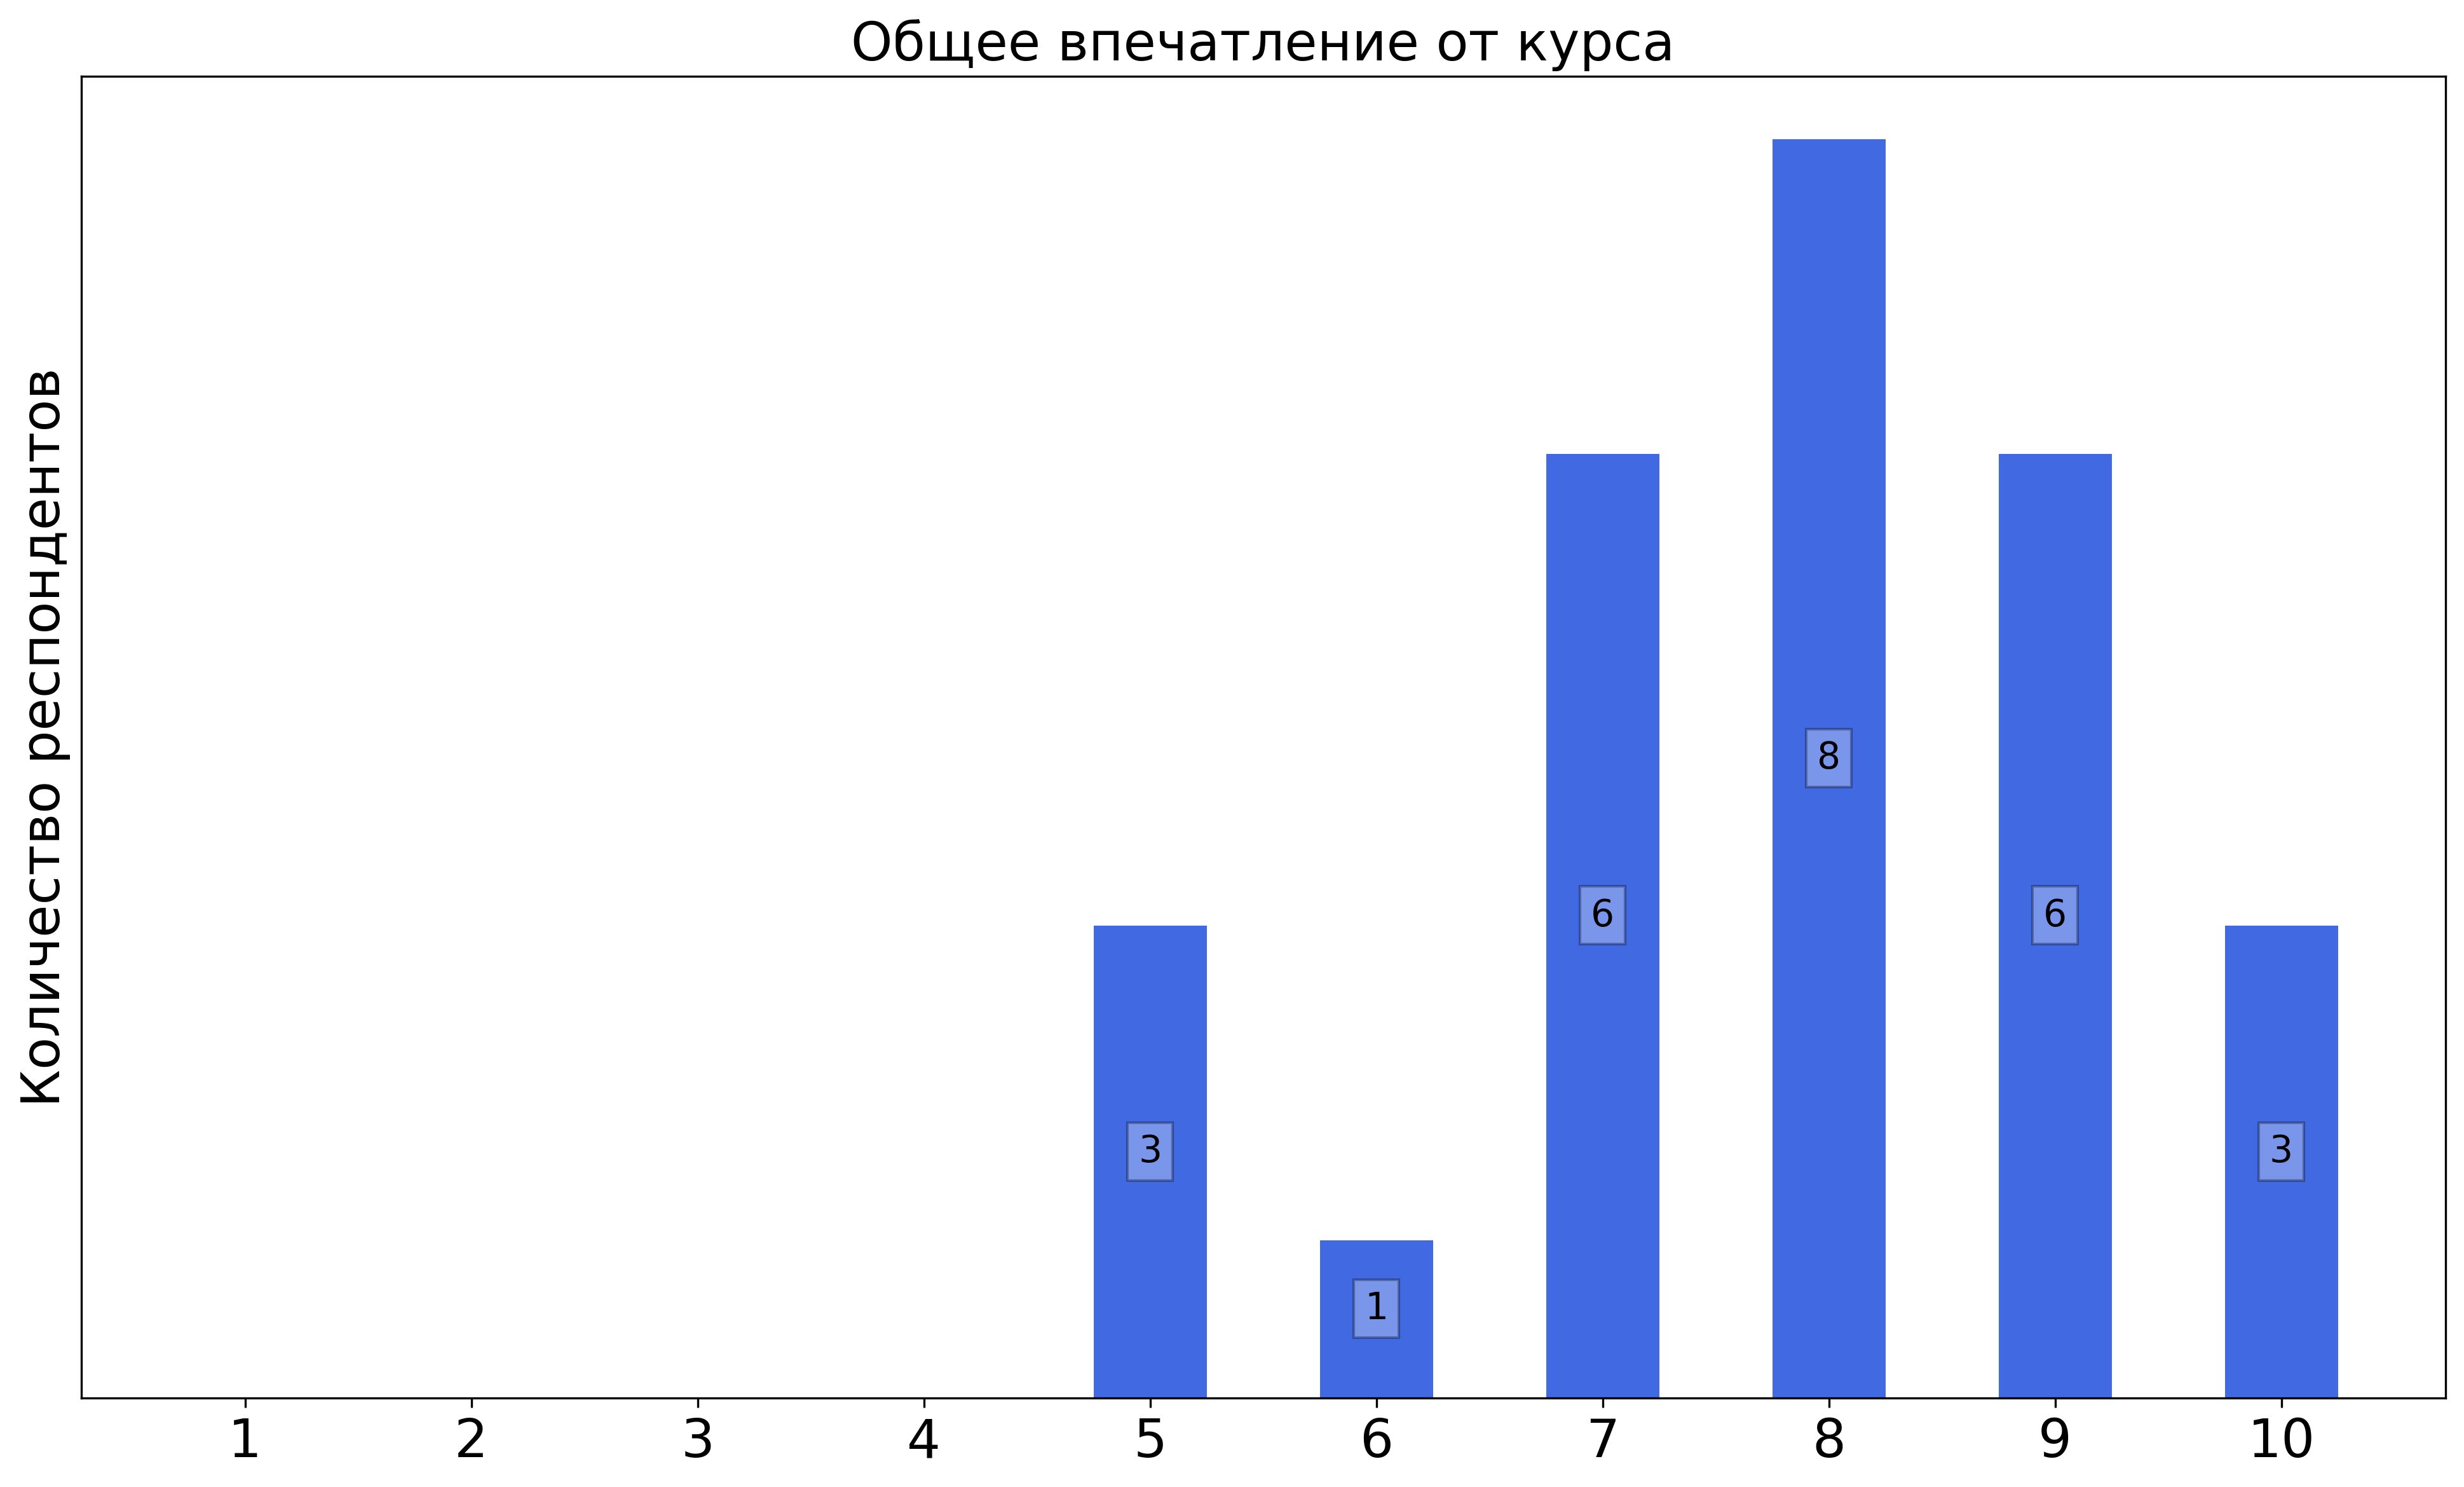
\includegraphics[width=\textwidth]{images/2 course/Общая физика - электричество и магнетизм/general-0.png}
			\end{subfigure}
			\begin{subfigure}[b]{0.45\textwidth}
				\centering
				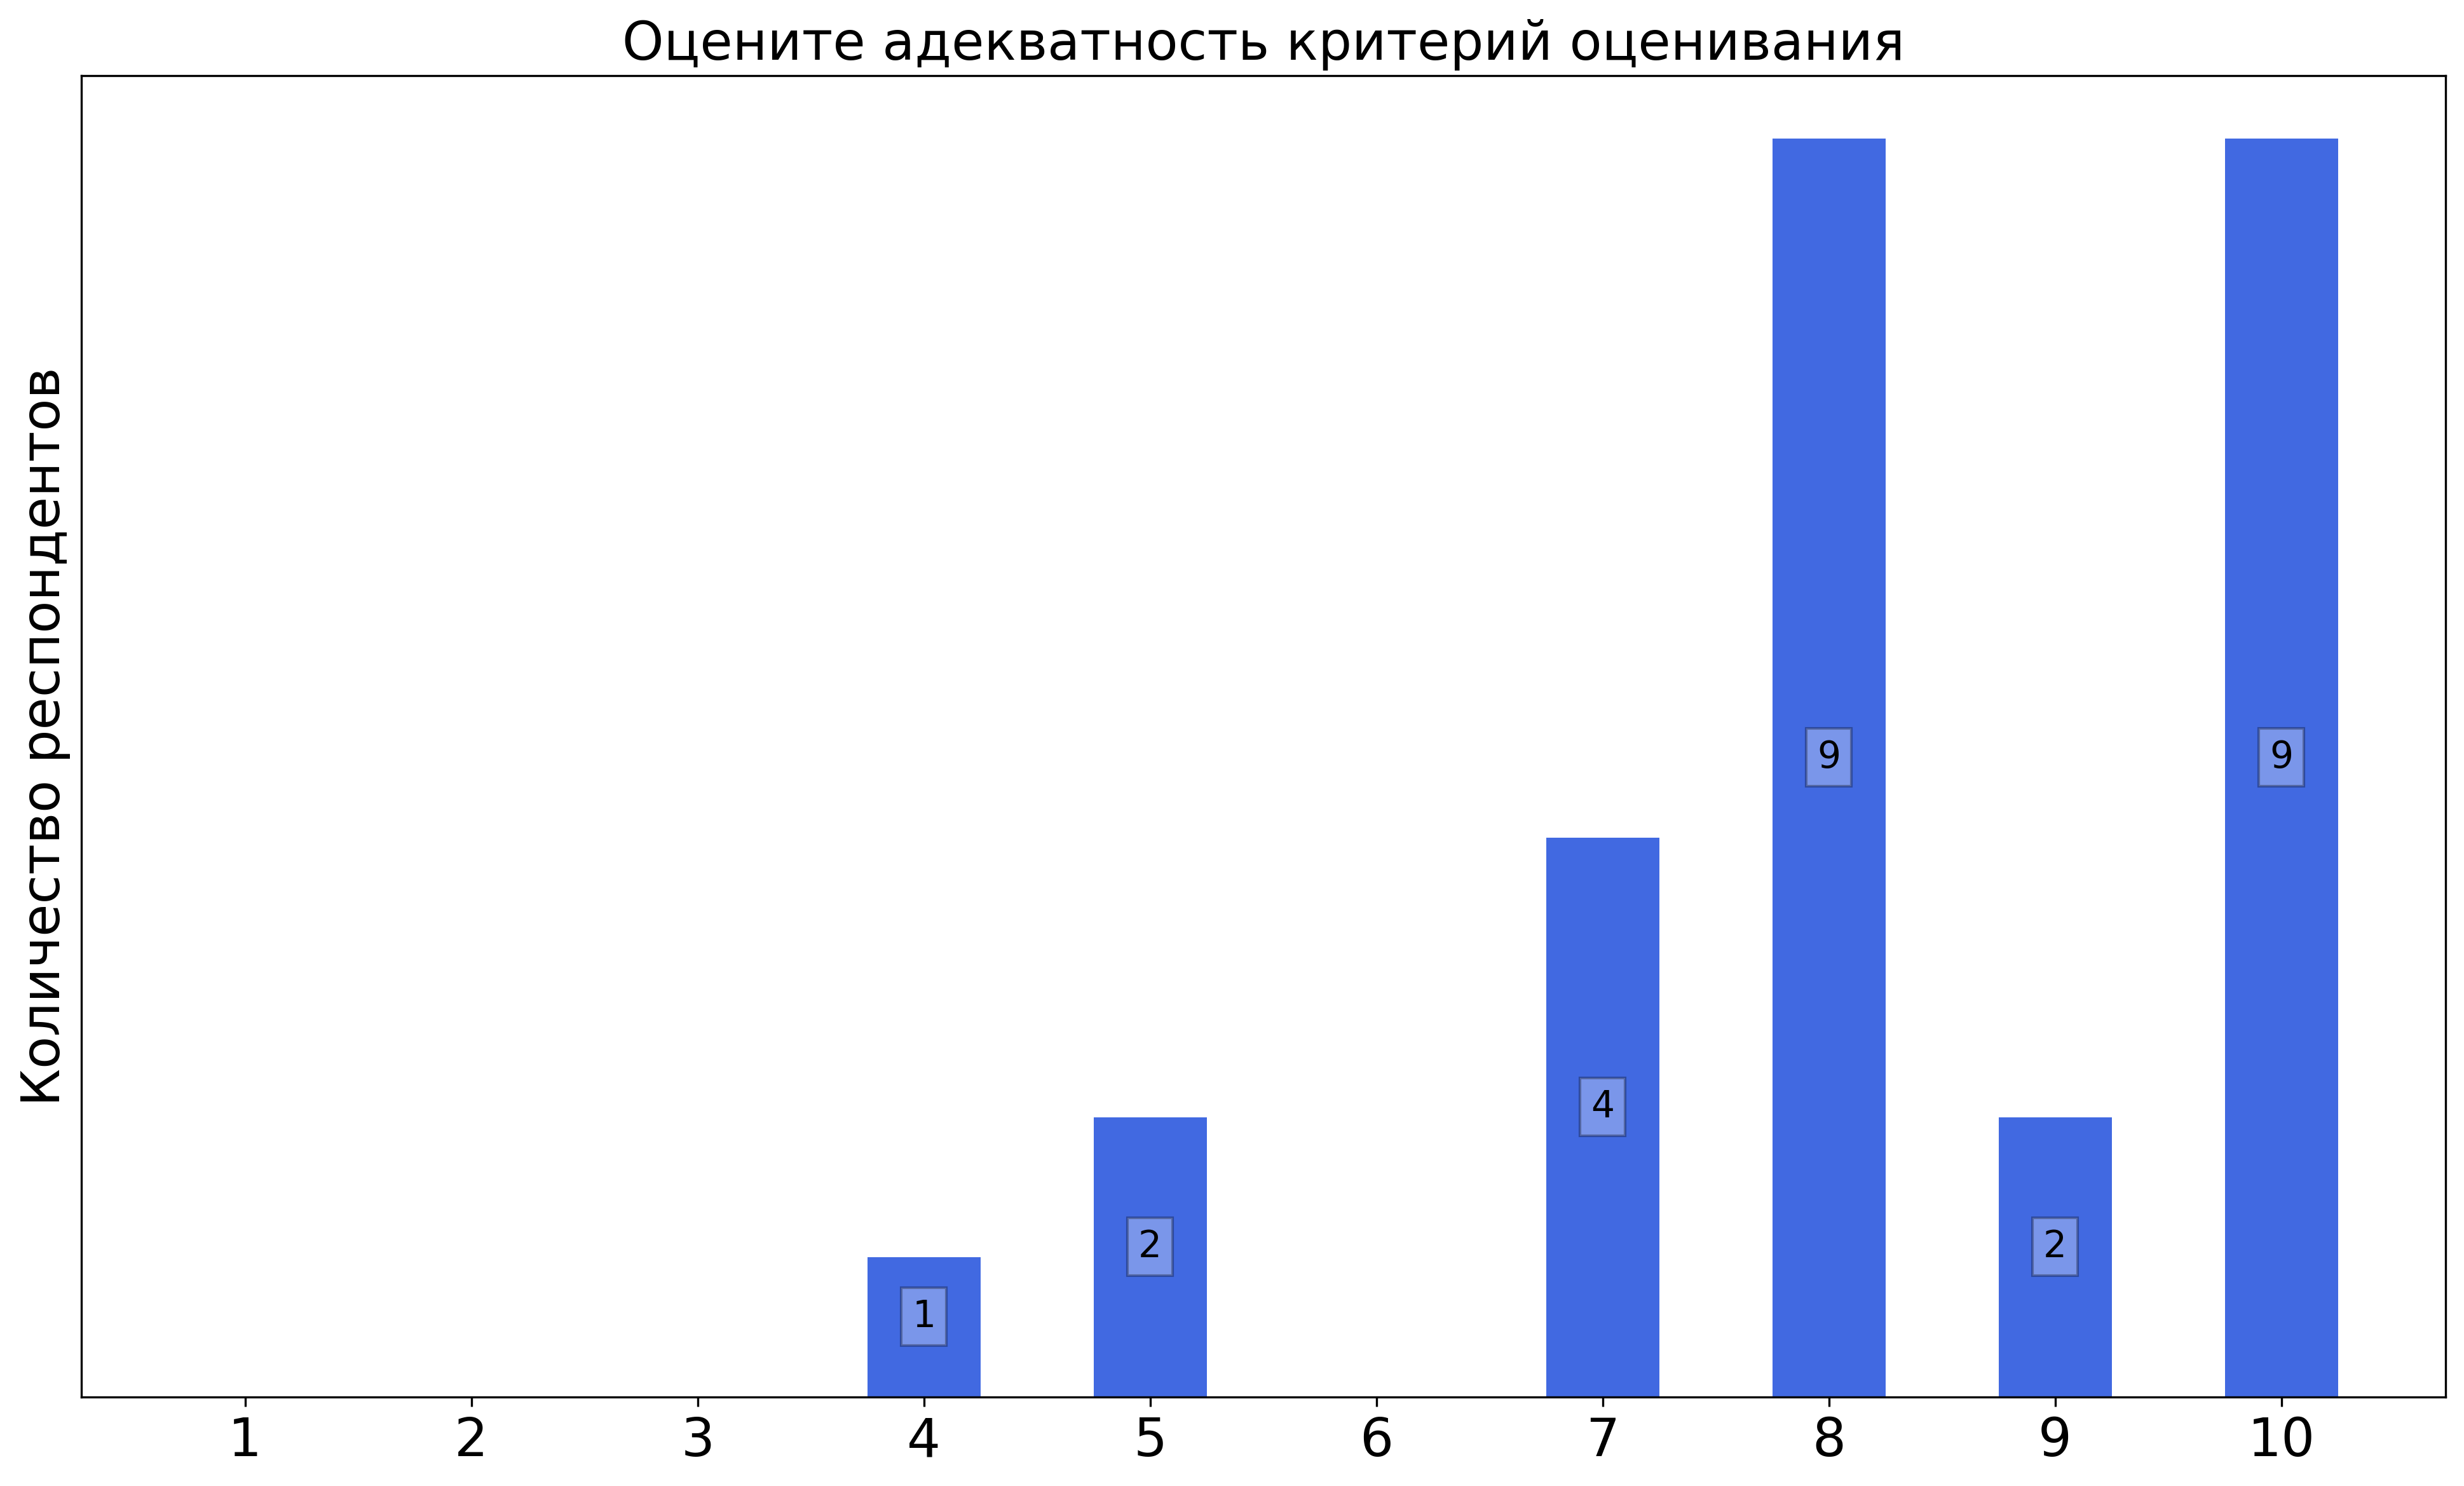
\includegraphics[width=\textwidth]{images/2 course/Общая физика - электричество и магнетизм/general-1.png}
			\end{subfigure}	
		\end{figure}

	\subsubsection{Материалы, использумые респондентами при изучении курса}

		\begin{figure}[H]
			\centering
			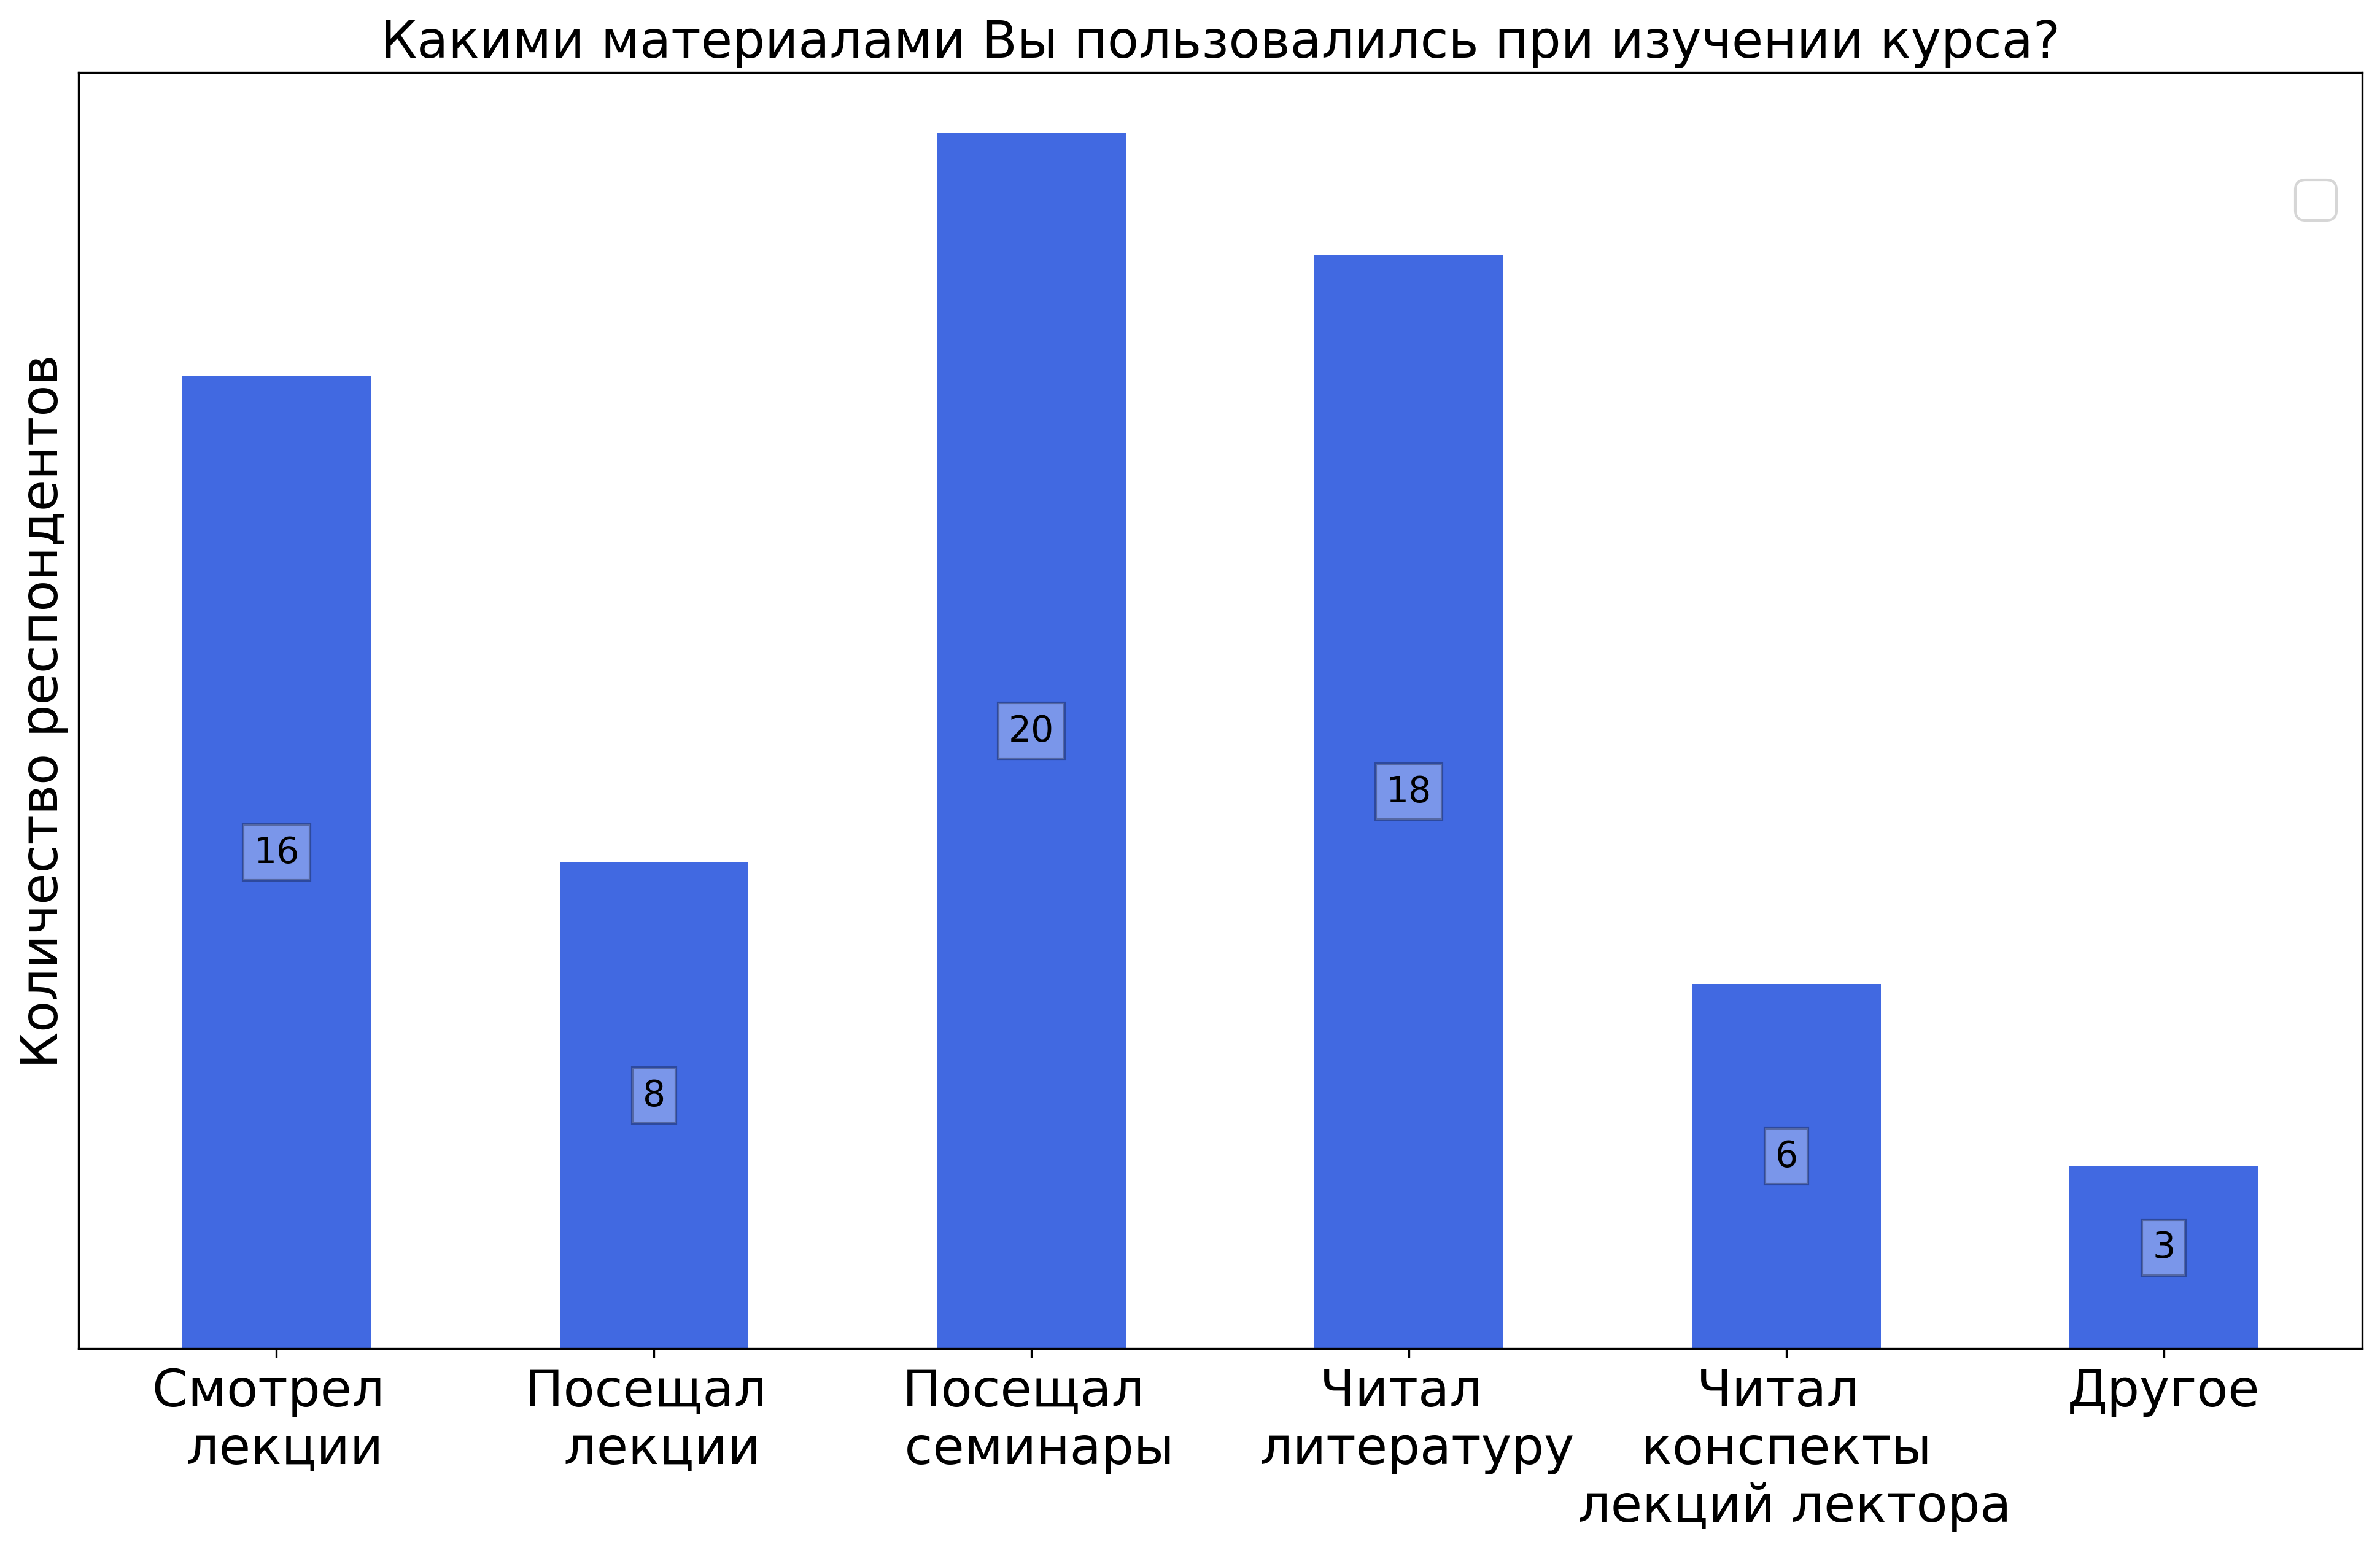
\includegraphics[width = 0.45\textwidth]{images/2 course/Общая физика - электричество и магнетизм/materials.png}
		\end{figure}

		\textit{В качестве других источников информации студенты указали:} 
		\begin{itemize}
			\item записи семинаров других преподавателей;
			\item доп. семинары Овчинкина В.А.
		\end{itemize}

	\subsubsection{Отзыв студентов о лекциях. Лектор: Овчинкин В.А.}

		\begin{figure}[H]
			\centering
            \begin{subfigure}[b]{0.45\textwidth}
				\centering
				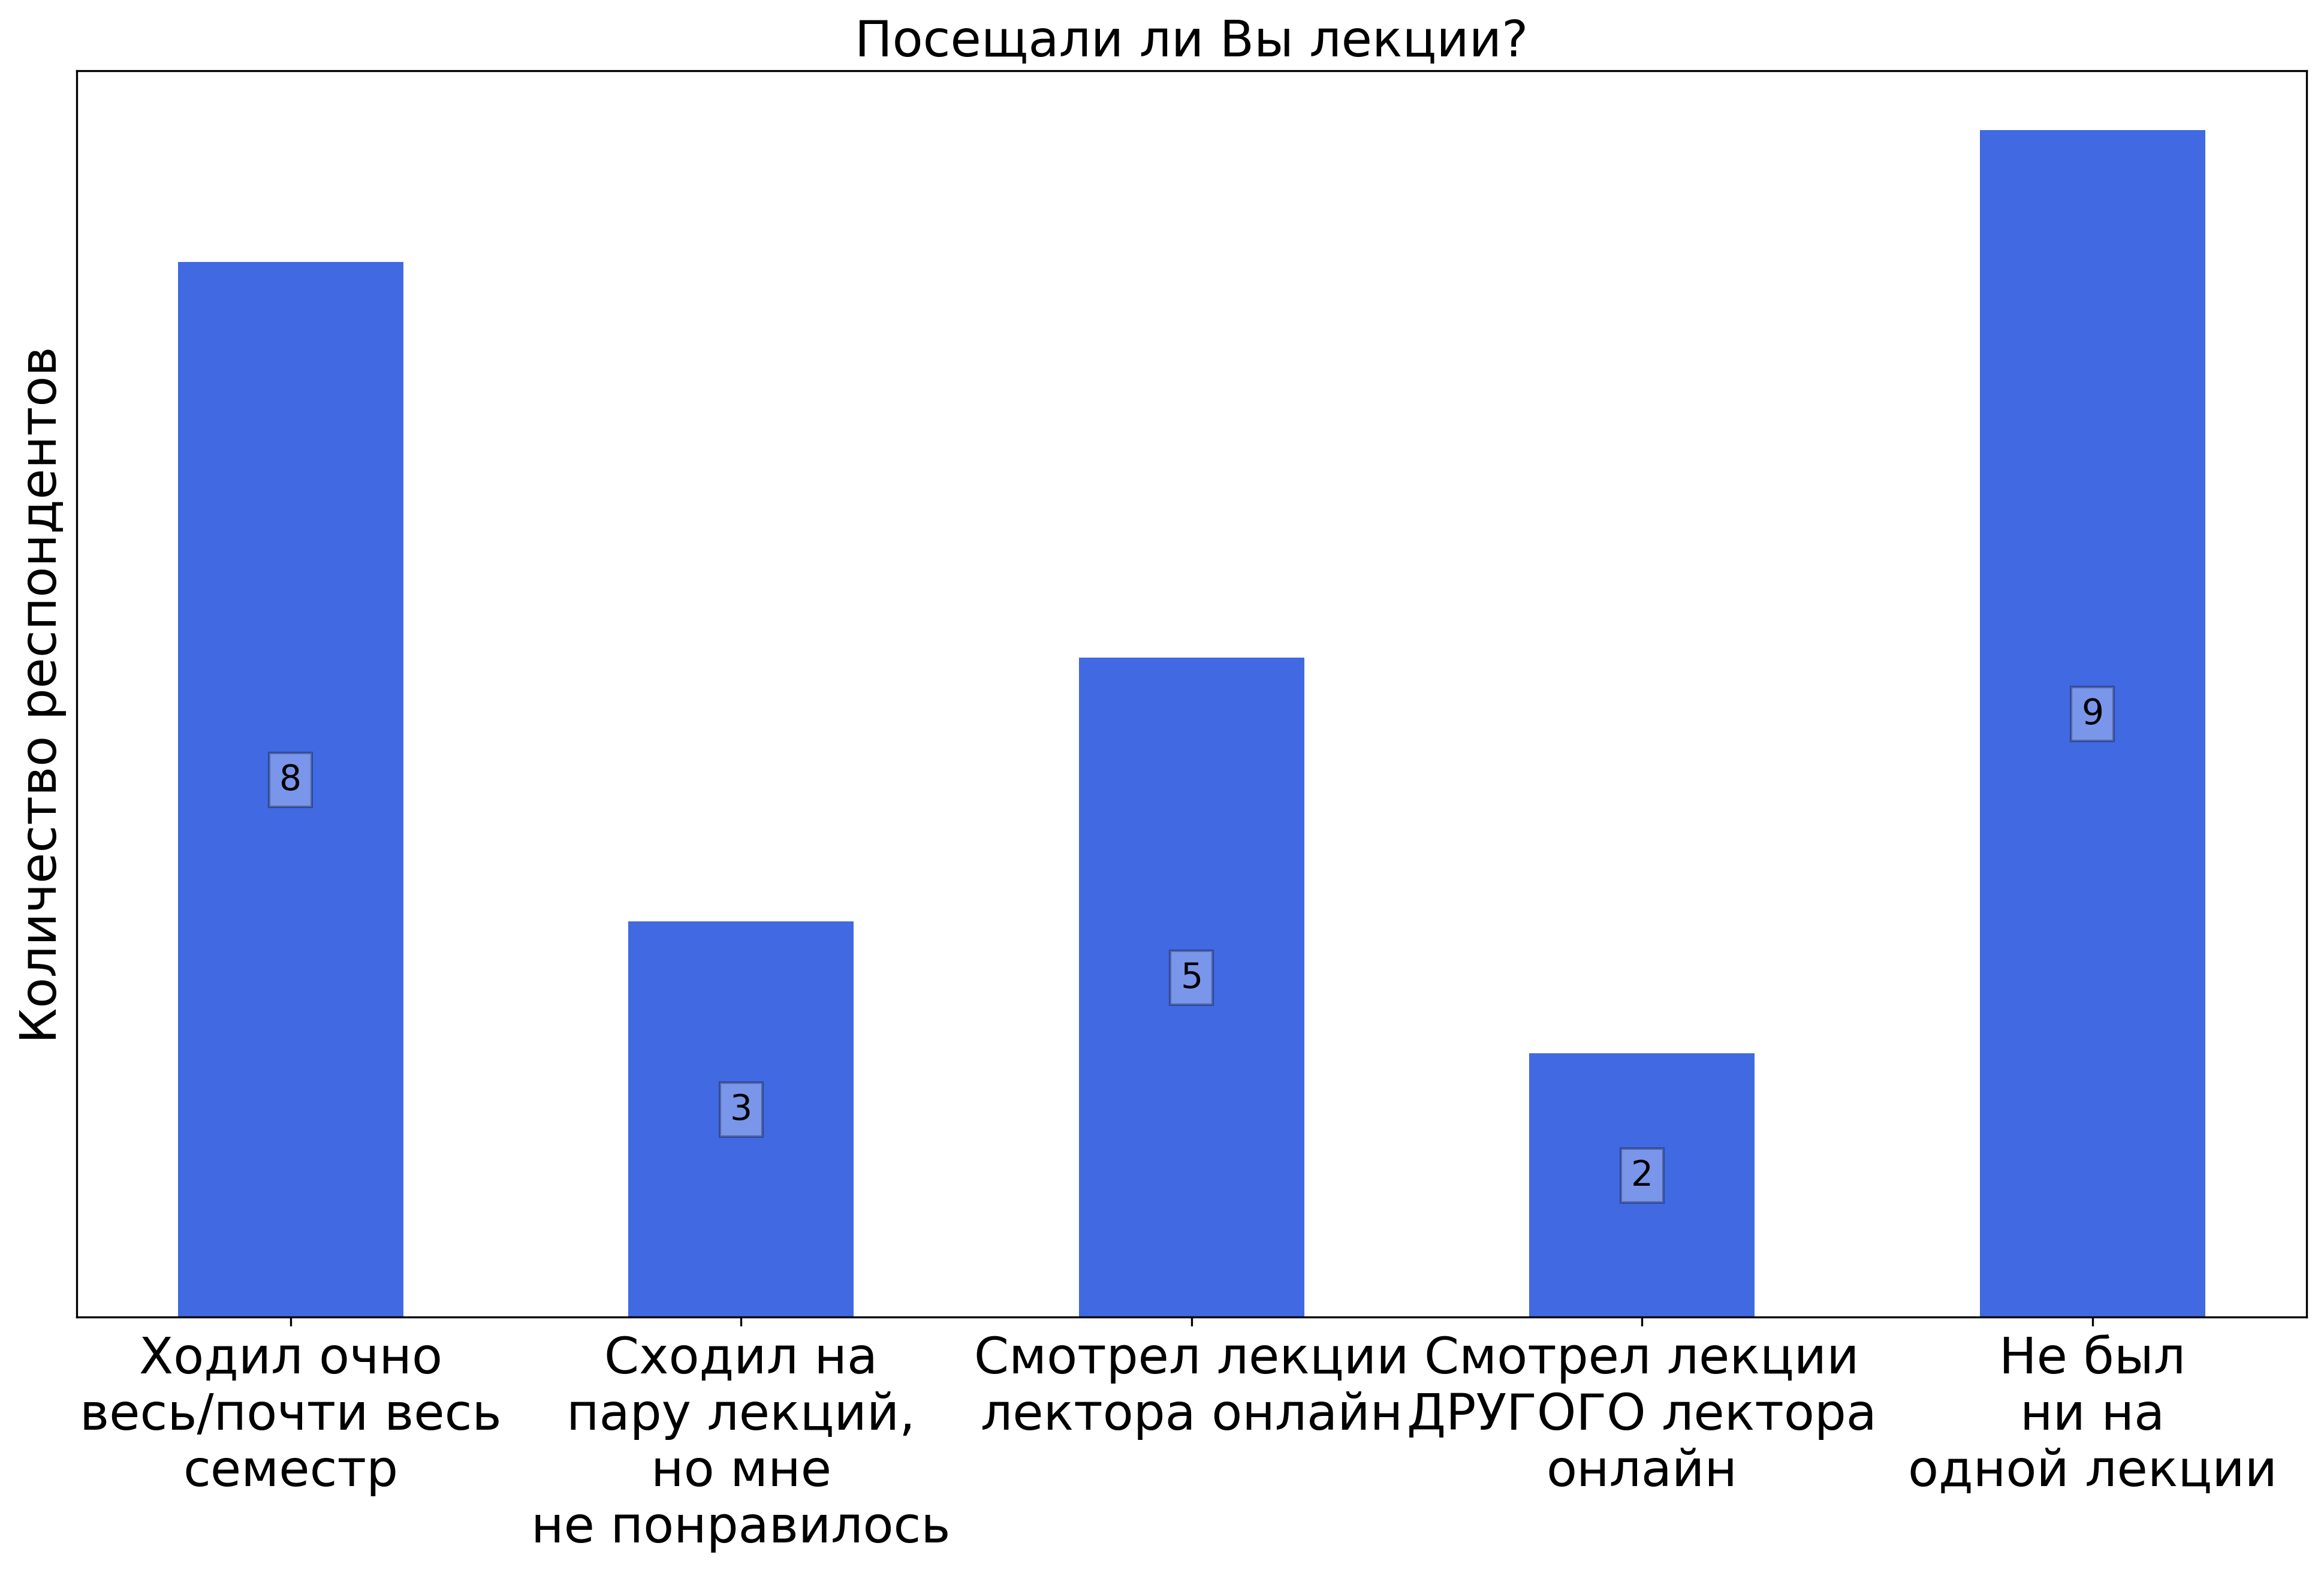
\includegraphics[width=\textwidth]{images/2 course/Общая физика - электричество и магнетизм/lecturer-questions-Овчинкин В.А.-0.png}
			\end{subfigure}
			\begin{subfigure}[b]{0.45\textwidth}
				\centering
				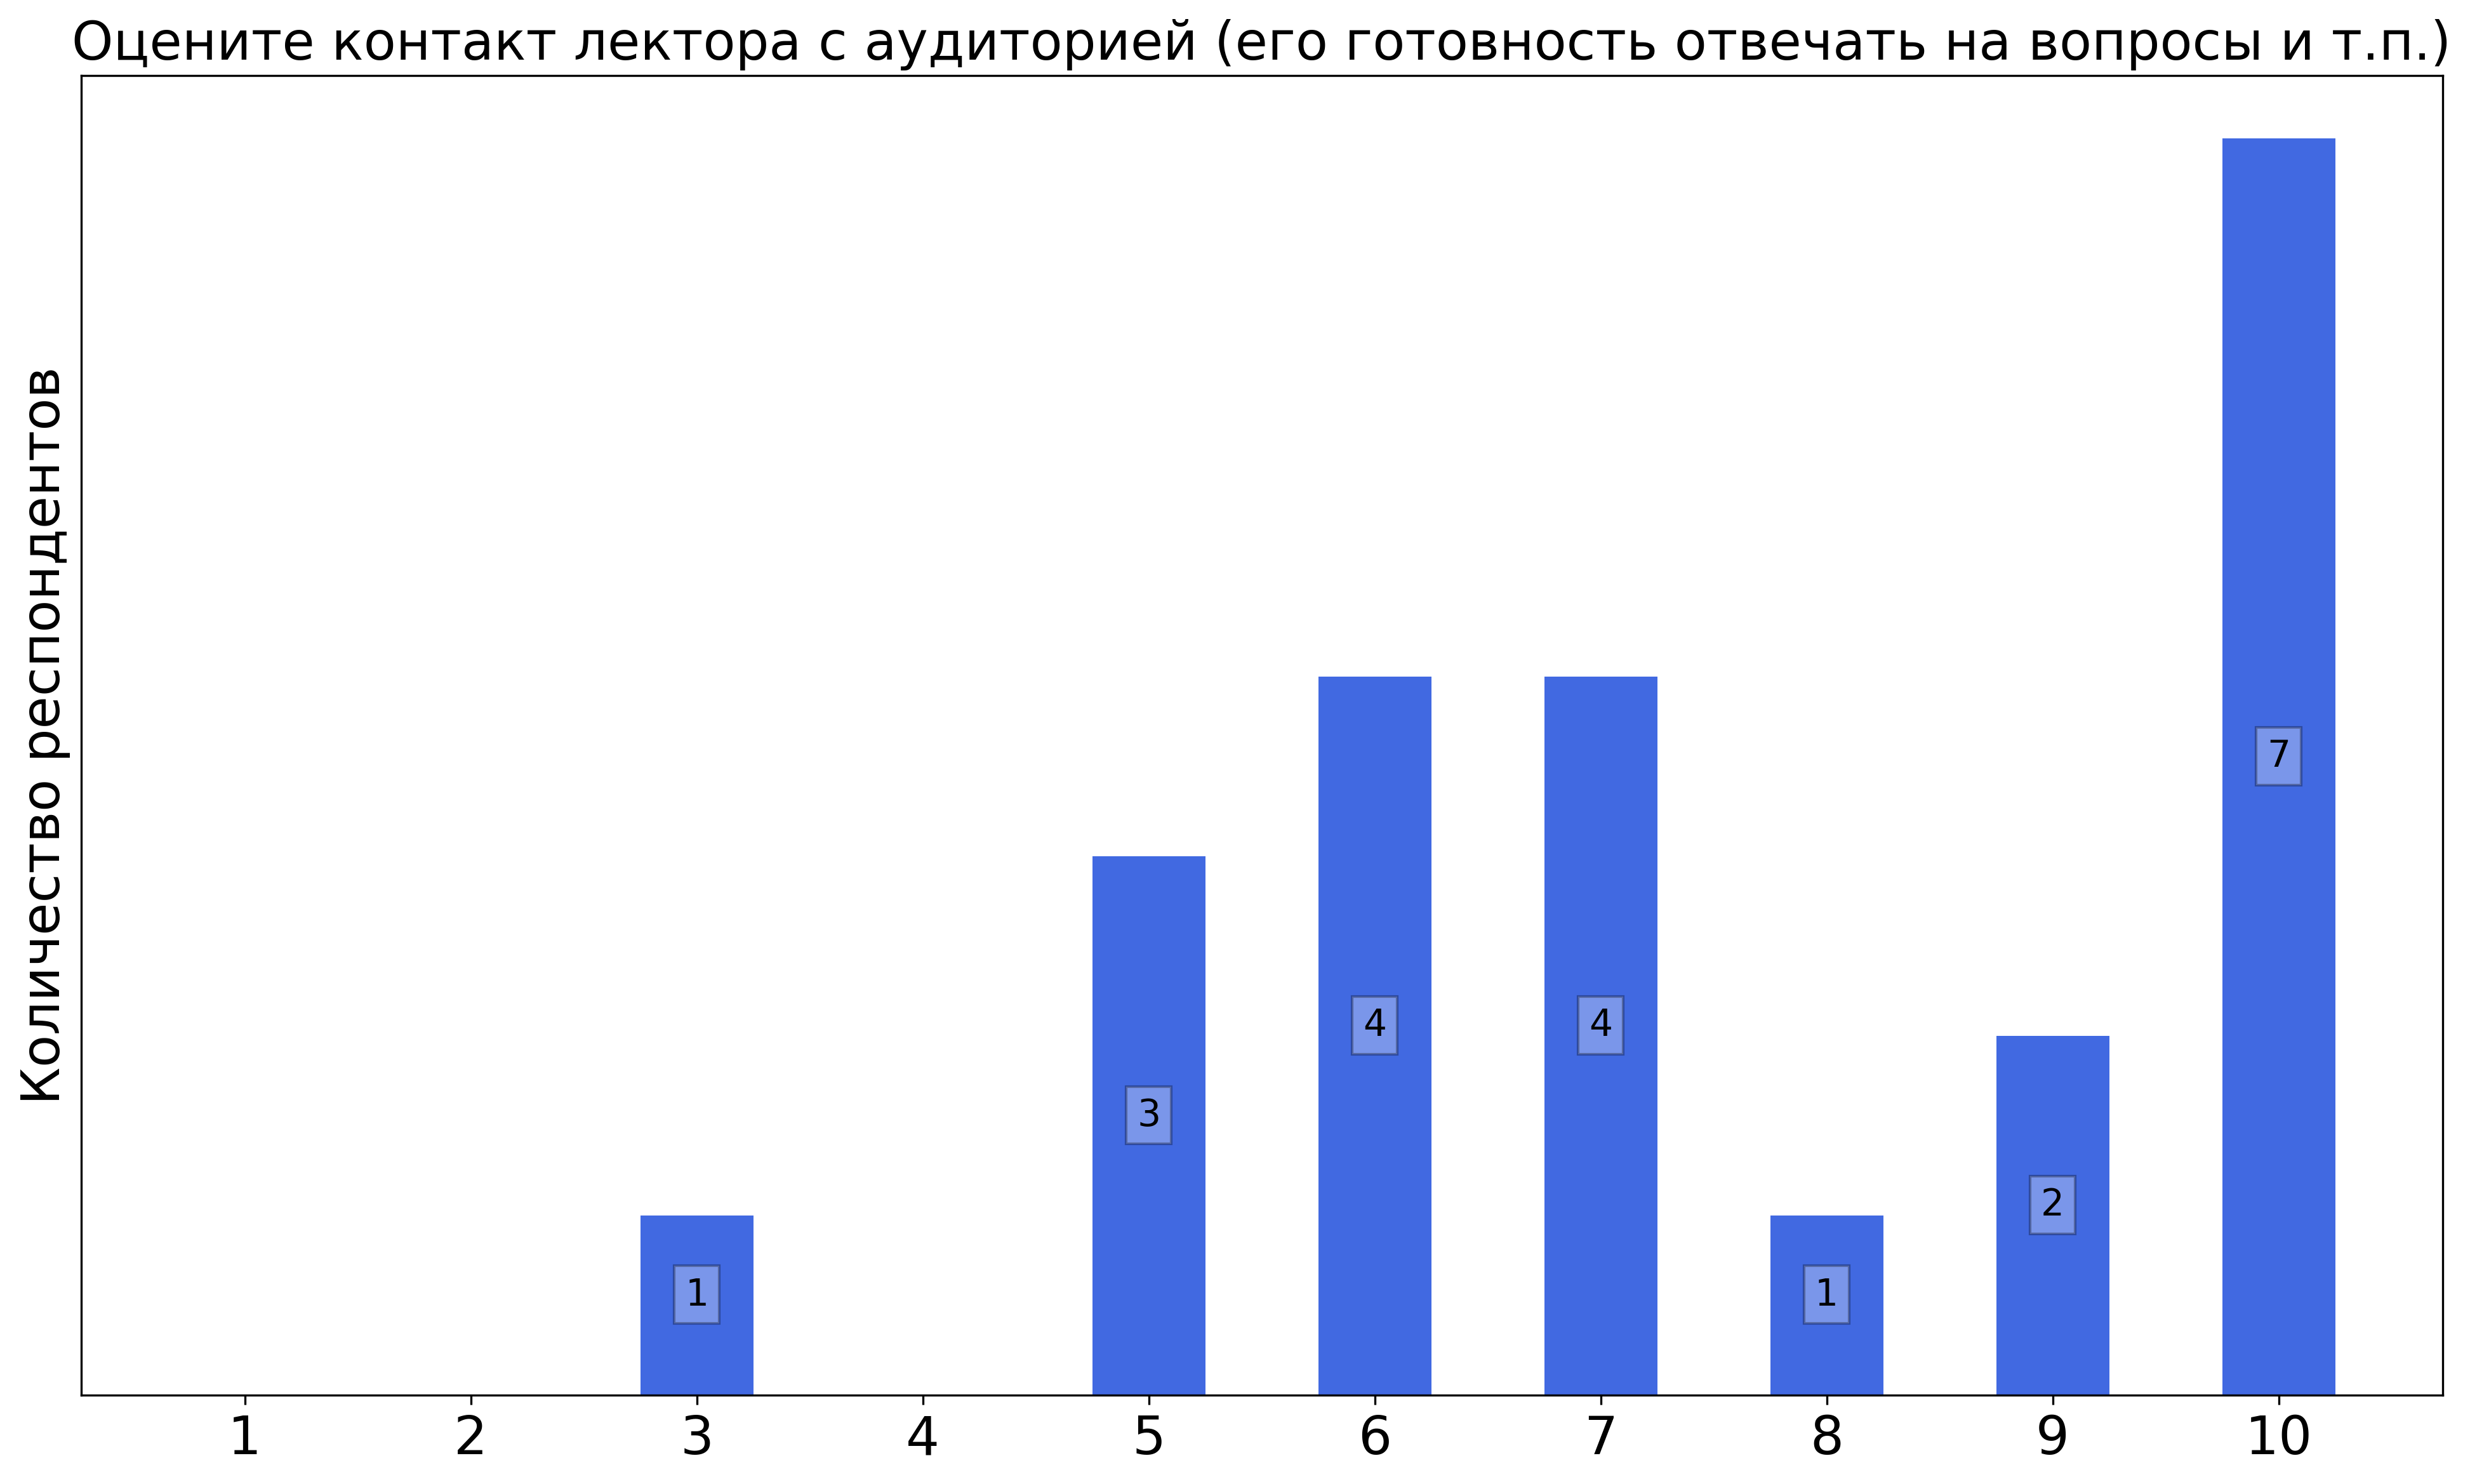
\includegraphics[width=\textwidth]{images/2 course/Общая физика - электричество и магнетизм/lecturer-marks-Овчинкин В.А.-0.png}
			\end{subfigure}
			\begin{subfigure}[b]{0.45\textwidth}
				\centering
				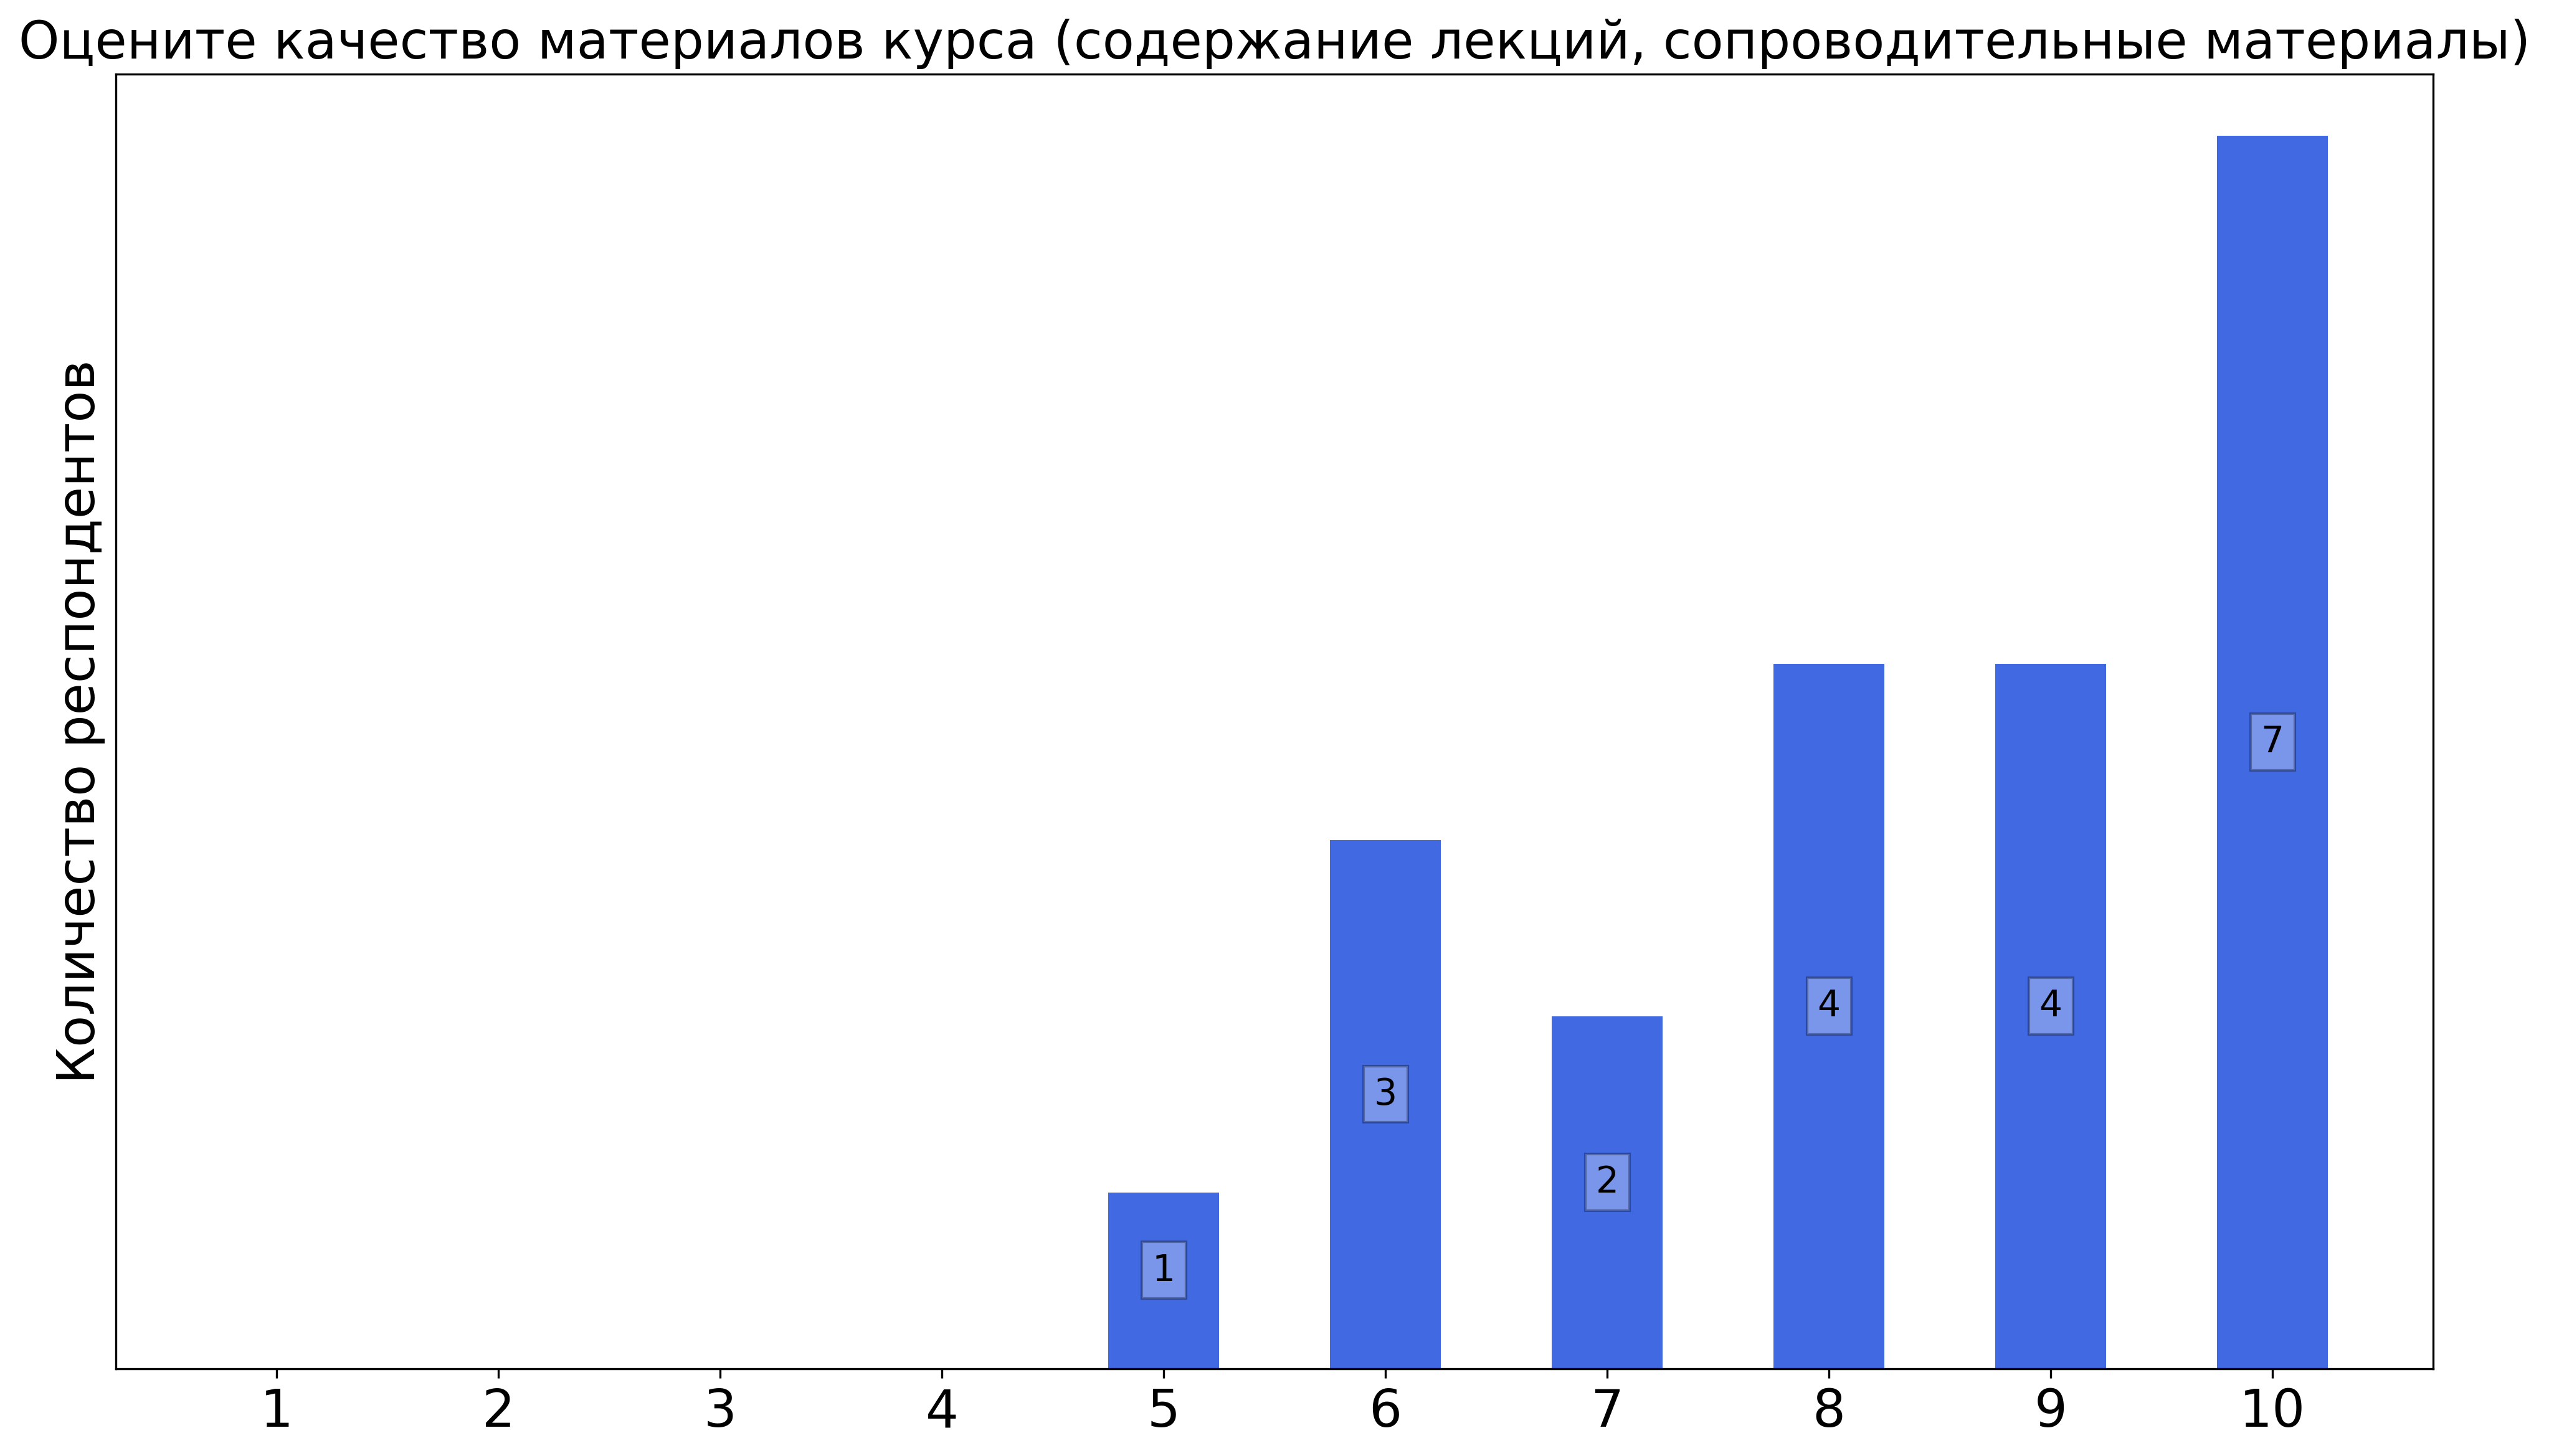
\includegraphics[width=\textwidth]{images/2 course/Общая физика - электричество и магнетизм/lecturer-marks-Овчинкин В.А.-1.png}
			\end{subfigure}
			\begin{subfigure}[b]{0.45\textwidth}
				\centering
				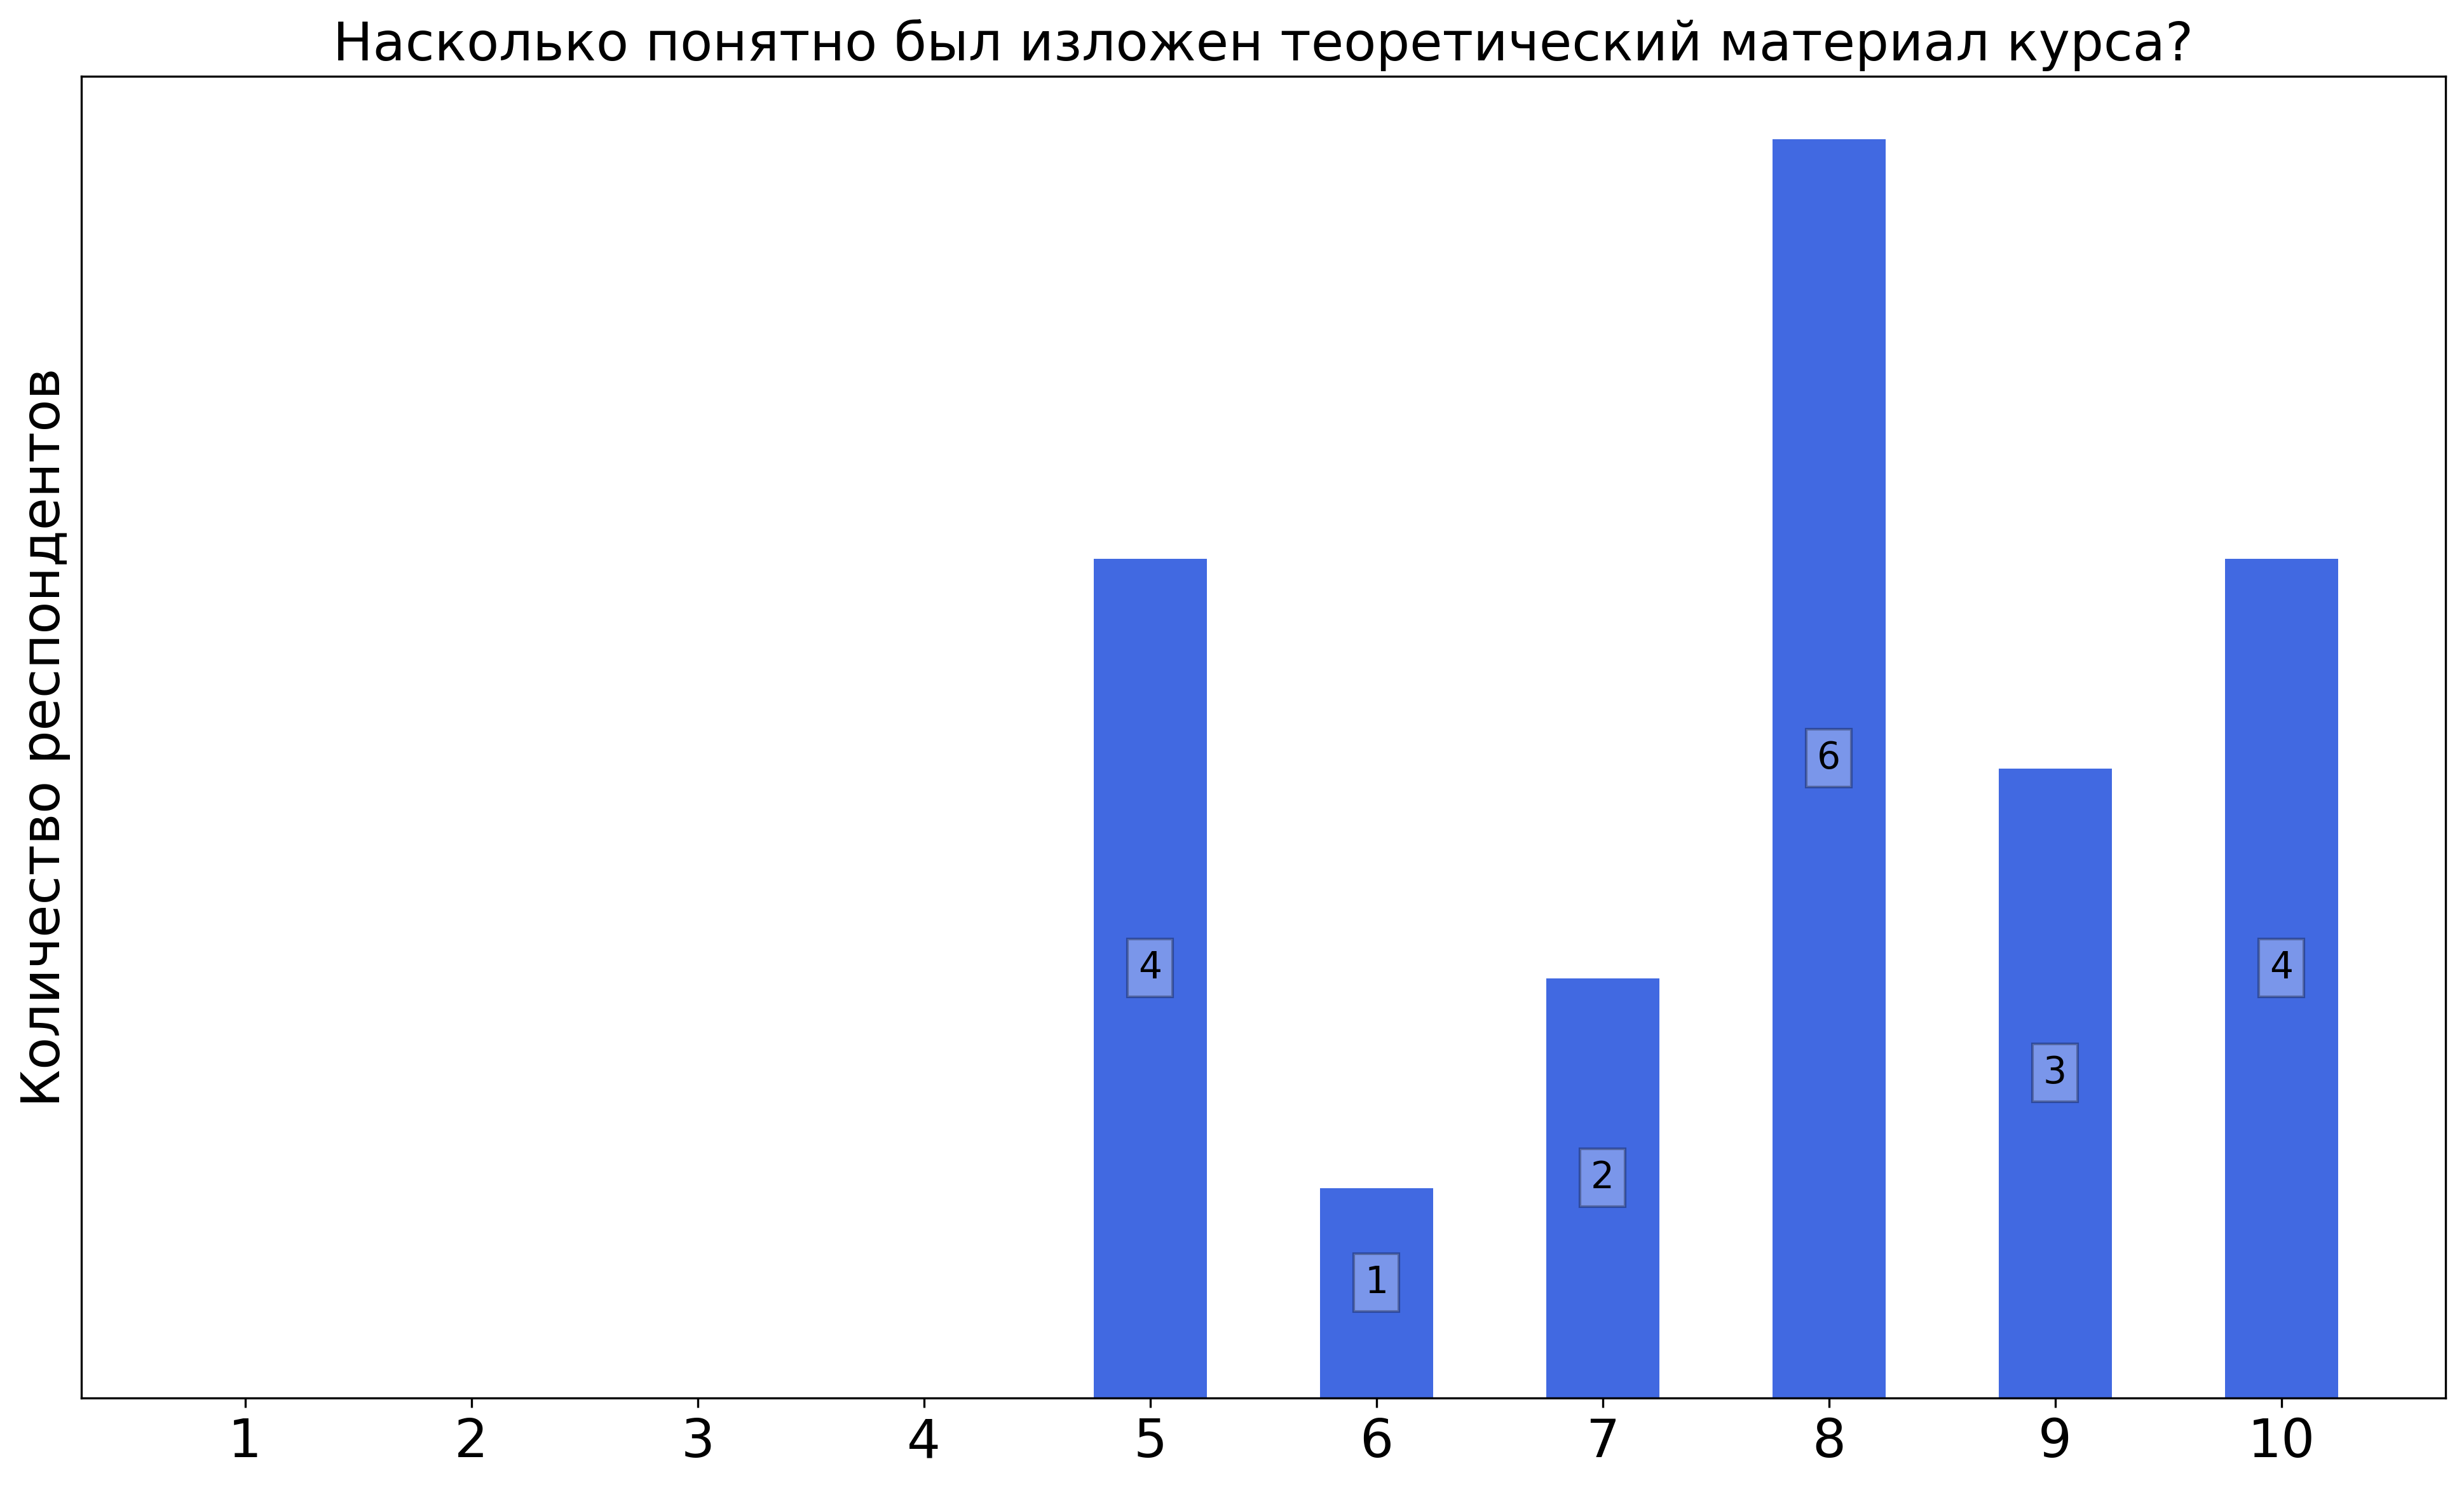
\includegraphics[width=\textwidth]{images/2 course/Общая физика - электричество и магнетизм/lecturer-marks-Овчинкин В.А.-2.png}
			\end{subfigure}	
			\begin{subfigure}[b]{0.45\textwidth}
				\centering
				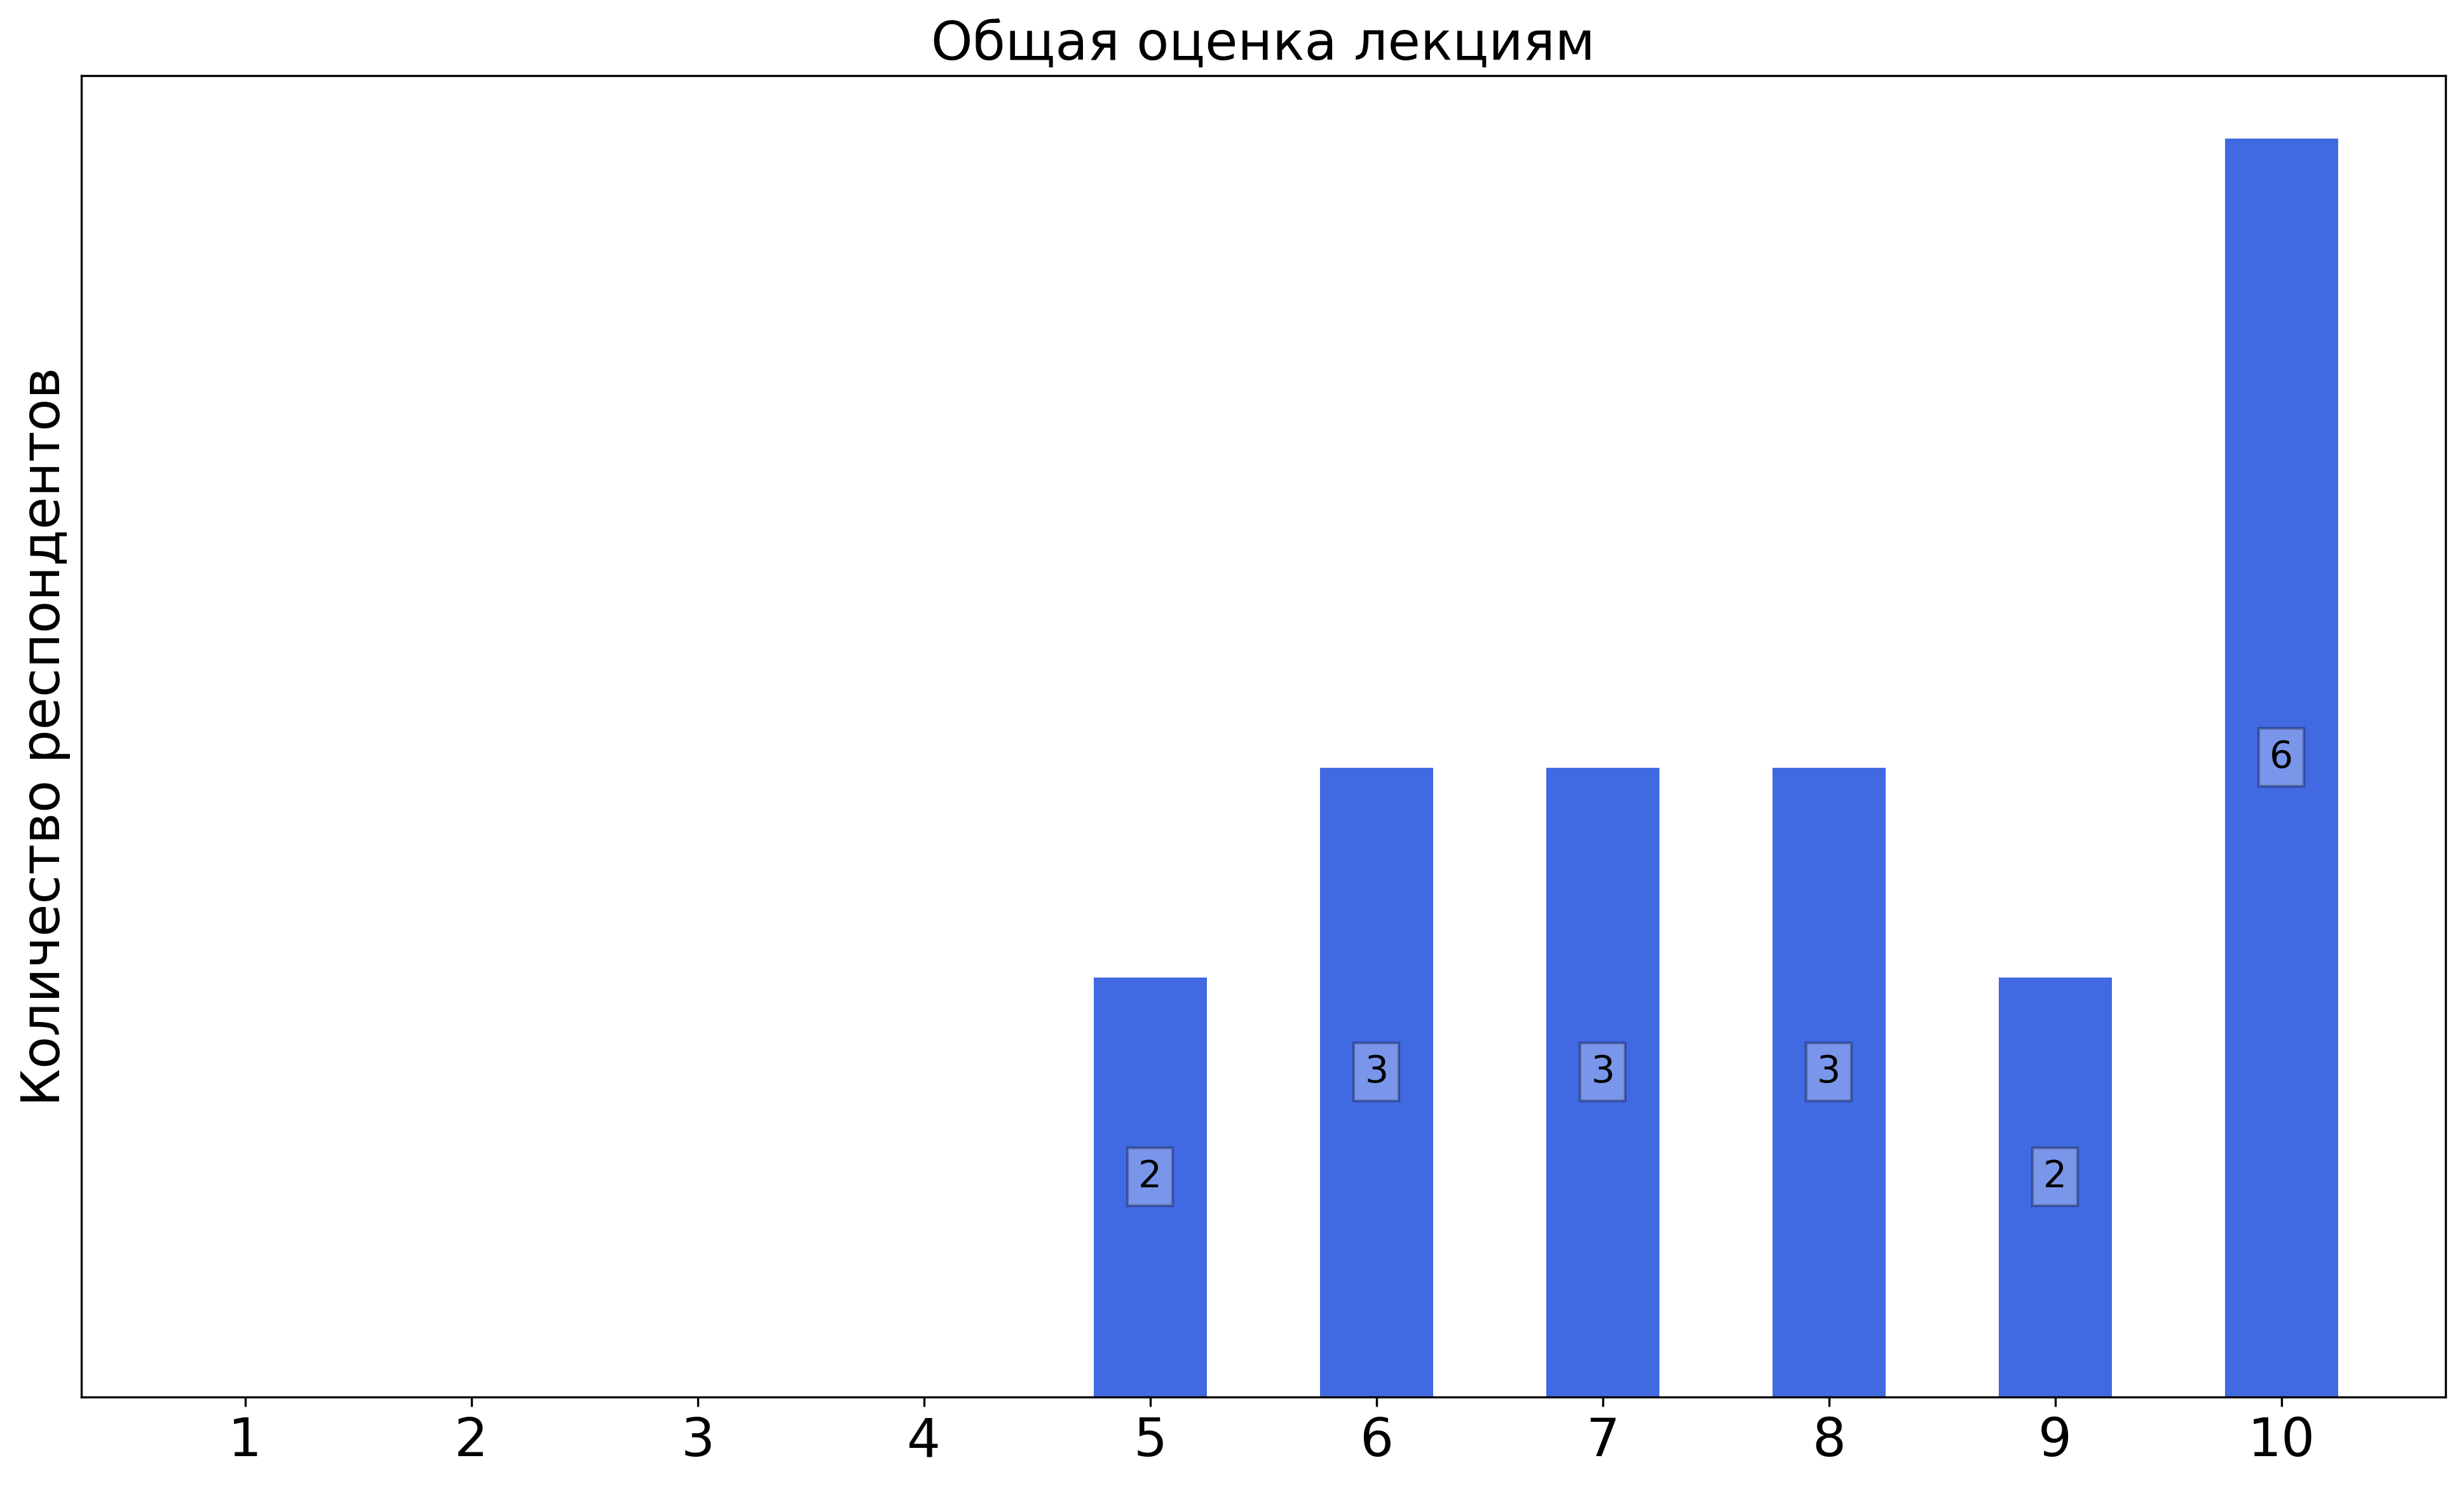
\includegraphics[width=\textwidth]{images/2 course/Общая физика - электричество и магнетизм/lecturer-marks-Овчинкин В.А.-3.png}
			\end{subfigure}
			\caption{Оценки респондентов о качестве преподавания лекций по курсу <<Общая физика: электричество и магнетизм>>}
		\end{figure}

		\textbf{Комментарии студентов о лекциях\protect\footnote{сохранены оригинальные орфография и пунктуация}}
			\begin{commentbox} 
				Базовичок 
			\end{commentbox} 
			
			\begin{commentbox} 
				не любит вопросы, но рассказывает хорошо 
			\end{commentbox} 
		
			\begin{commentbox} 
				В течение семестра не хватало учебного пособия от лектора по его лекциям  
			\end{commentbox} 
		
			\begin{commentbox} 
				Читает с листка, переписывает на доску и агрессивно относится к вопросам 
			\end{commentbox} 
    
    
    \subsubsection{Отзыв студентов о семинарах. Семинарист: Долгих В.А.}
		\begin{figure}[H]
			\centering
			\begin{subfigure}[b]{0.45\textwidth}
				\centering
				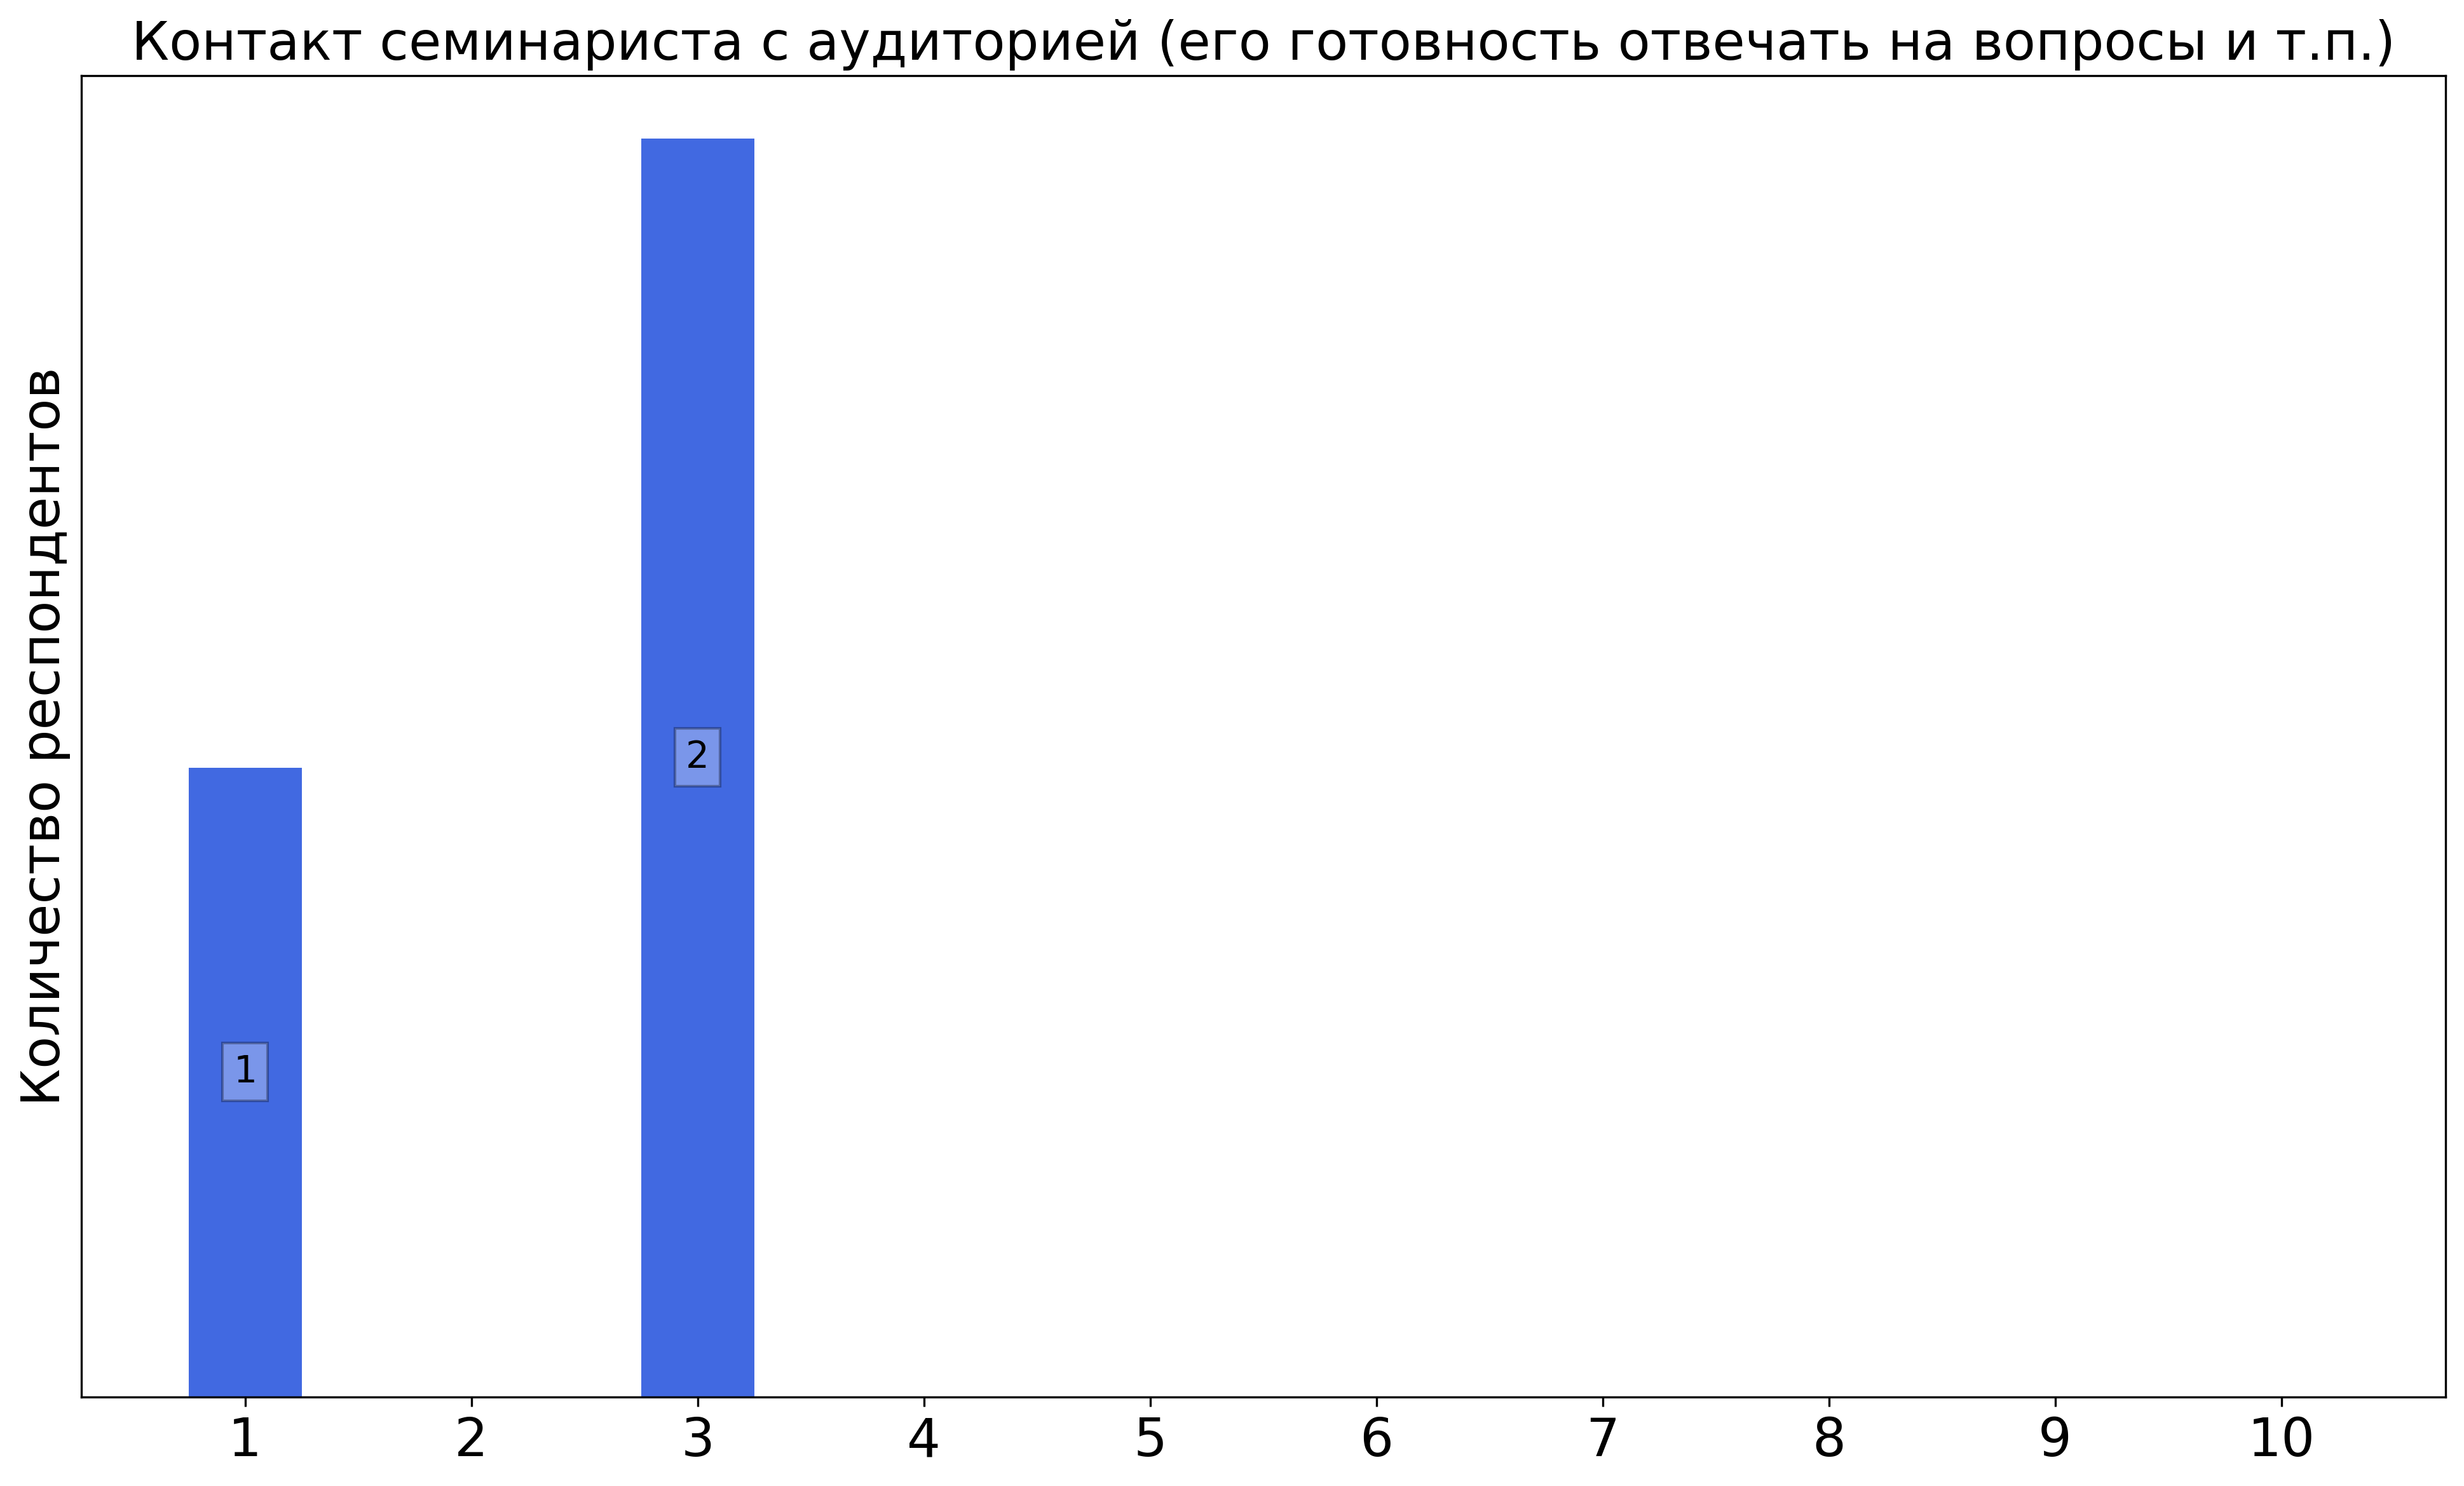
\includegraphics[width=\textwidth]{images/2 course/Общая физика - электричество и магнетизм/seminarists-marks-Долгих В.А.-0.png}
			\end{subfigure}
			\begin{subfigure}[b]{0.45\textwidth}
				\centering
				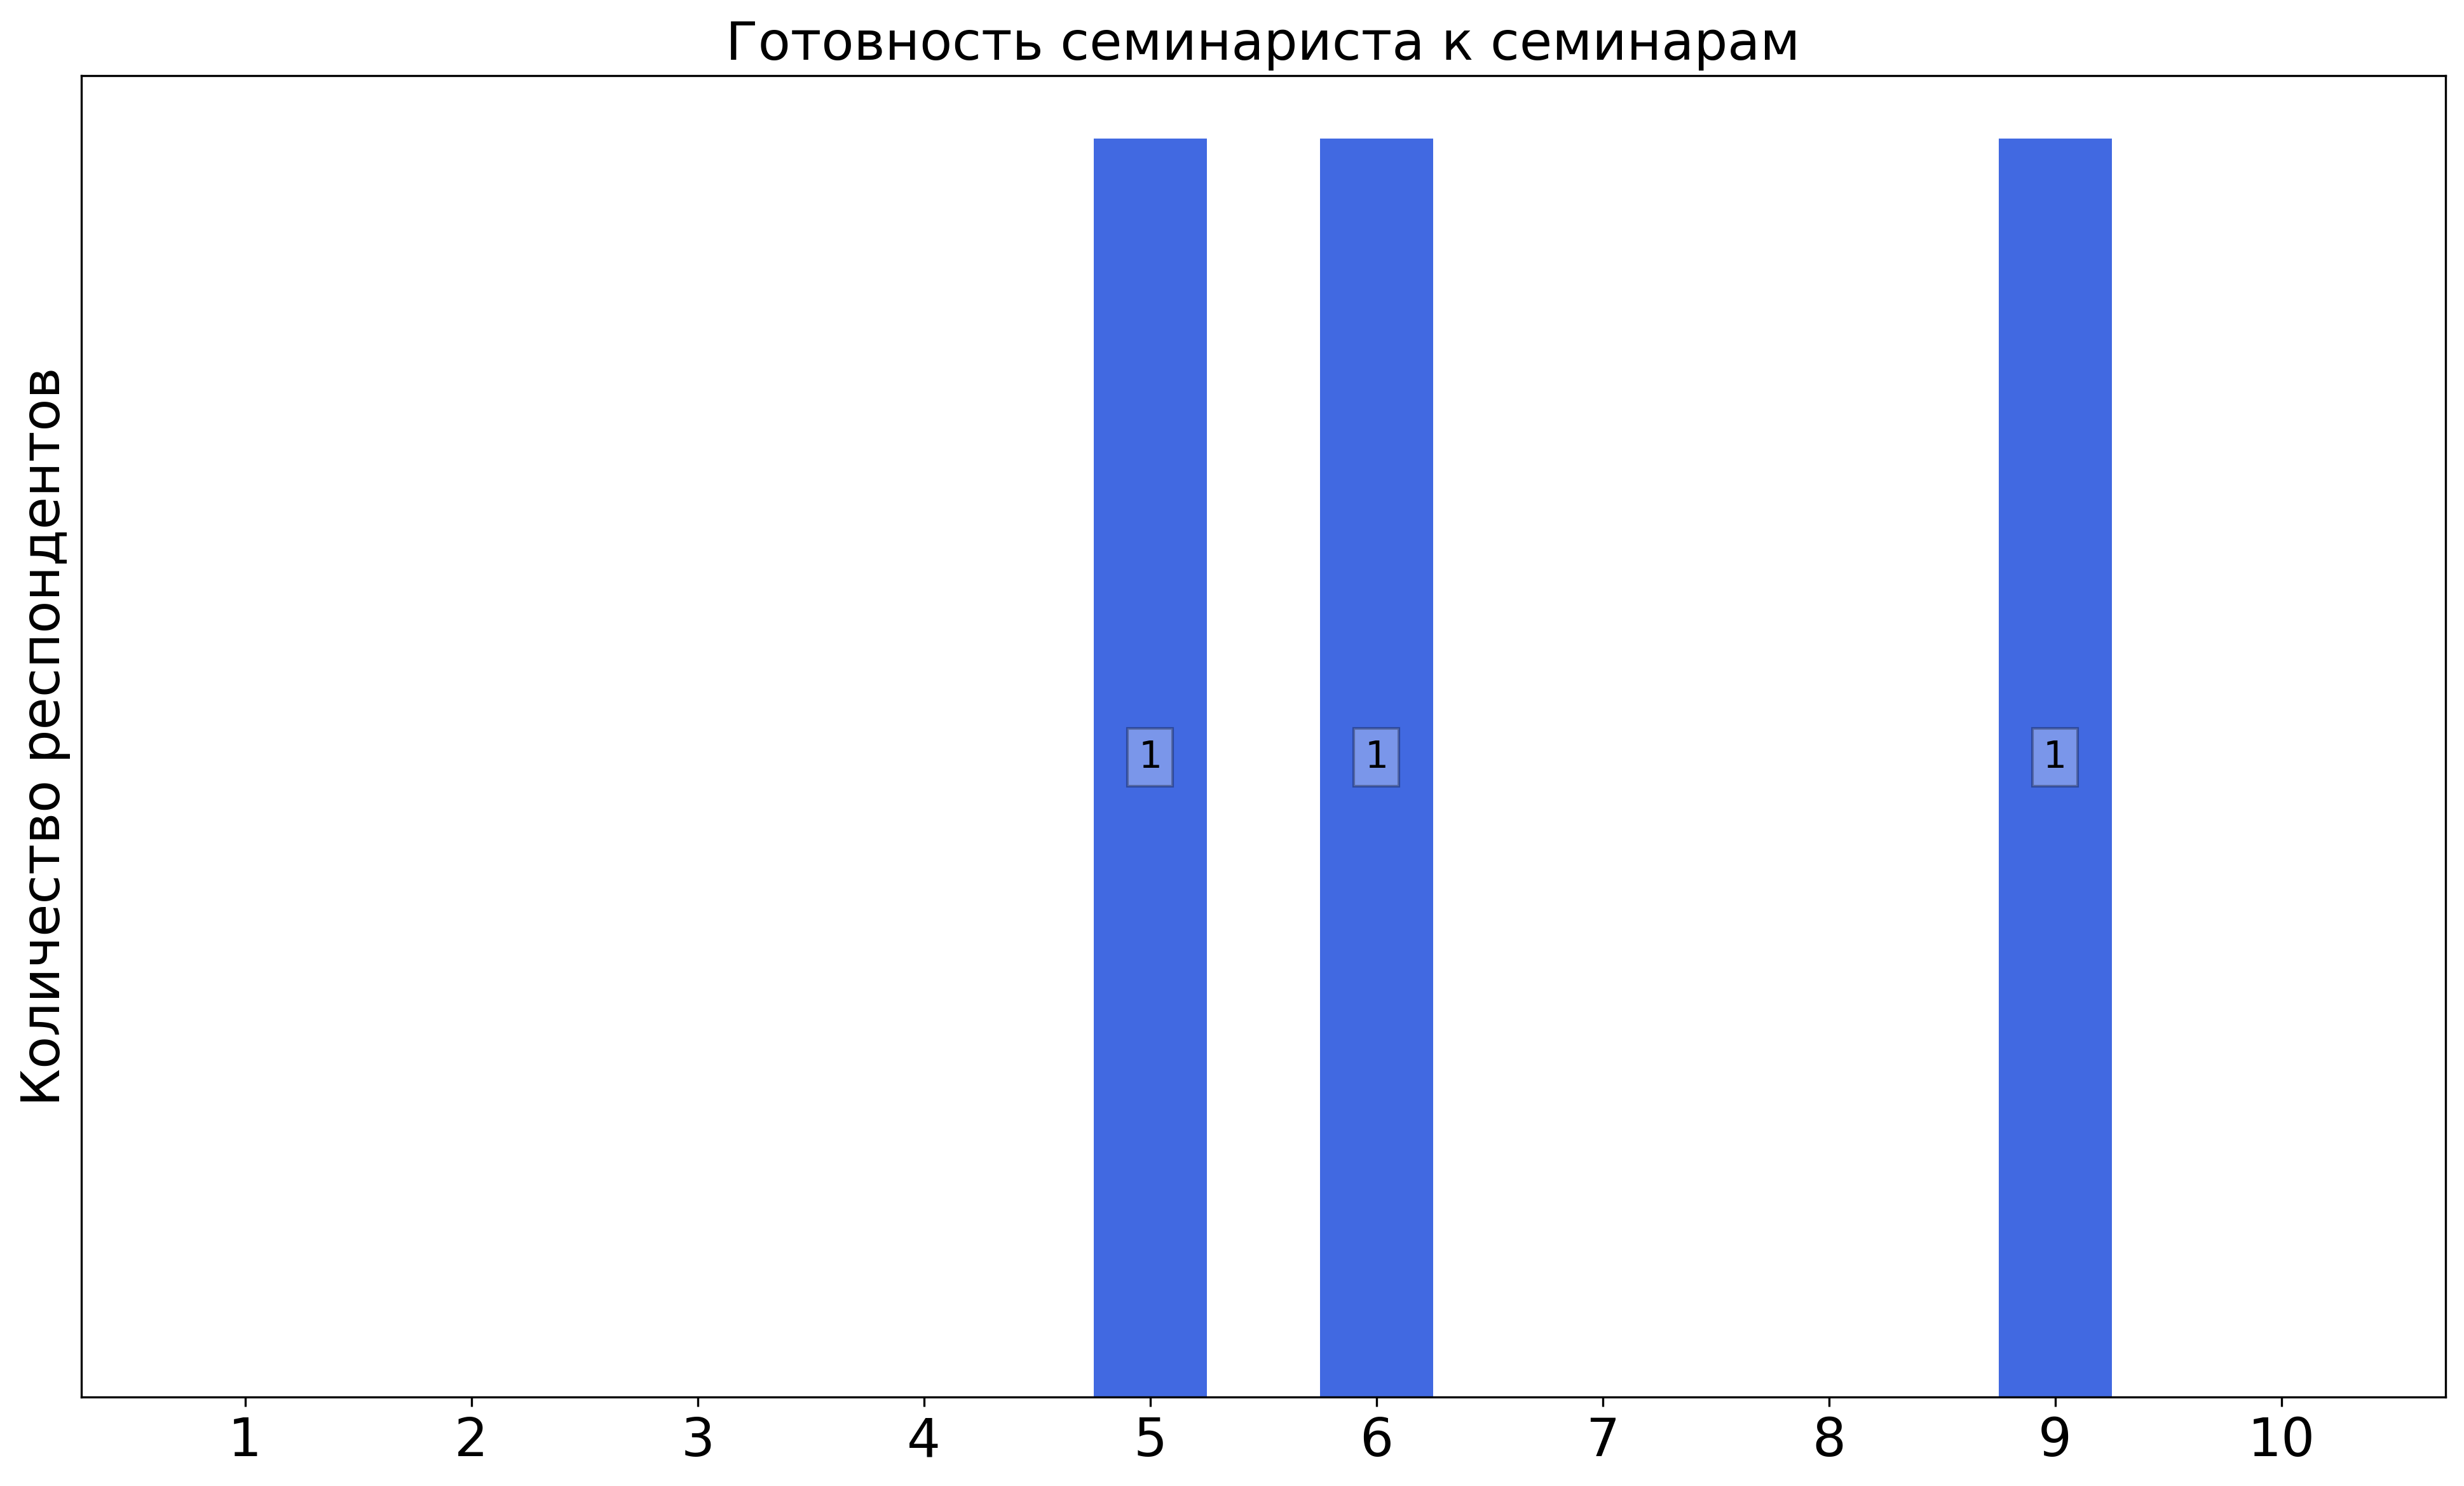
\includegraphics[width=\textwidth]{images/2 course/Общая физика - электричество и магнетизм/seminarists-marks-Долгих В.А.-1.png}
			\end{subfigure}
			\begin{subfigure}[b]{0.45\textwidth}
				\centering
				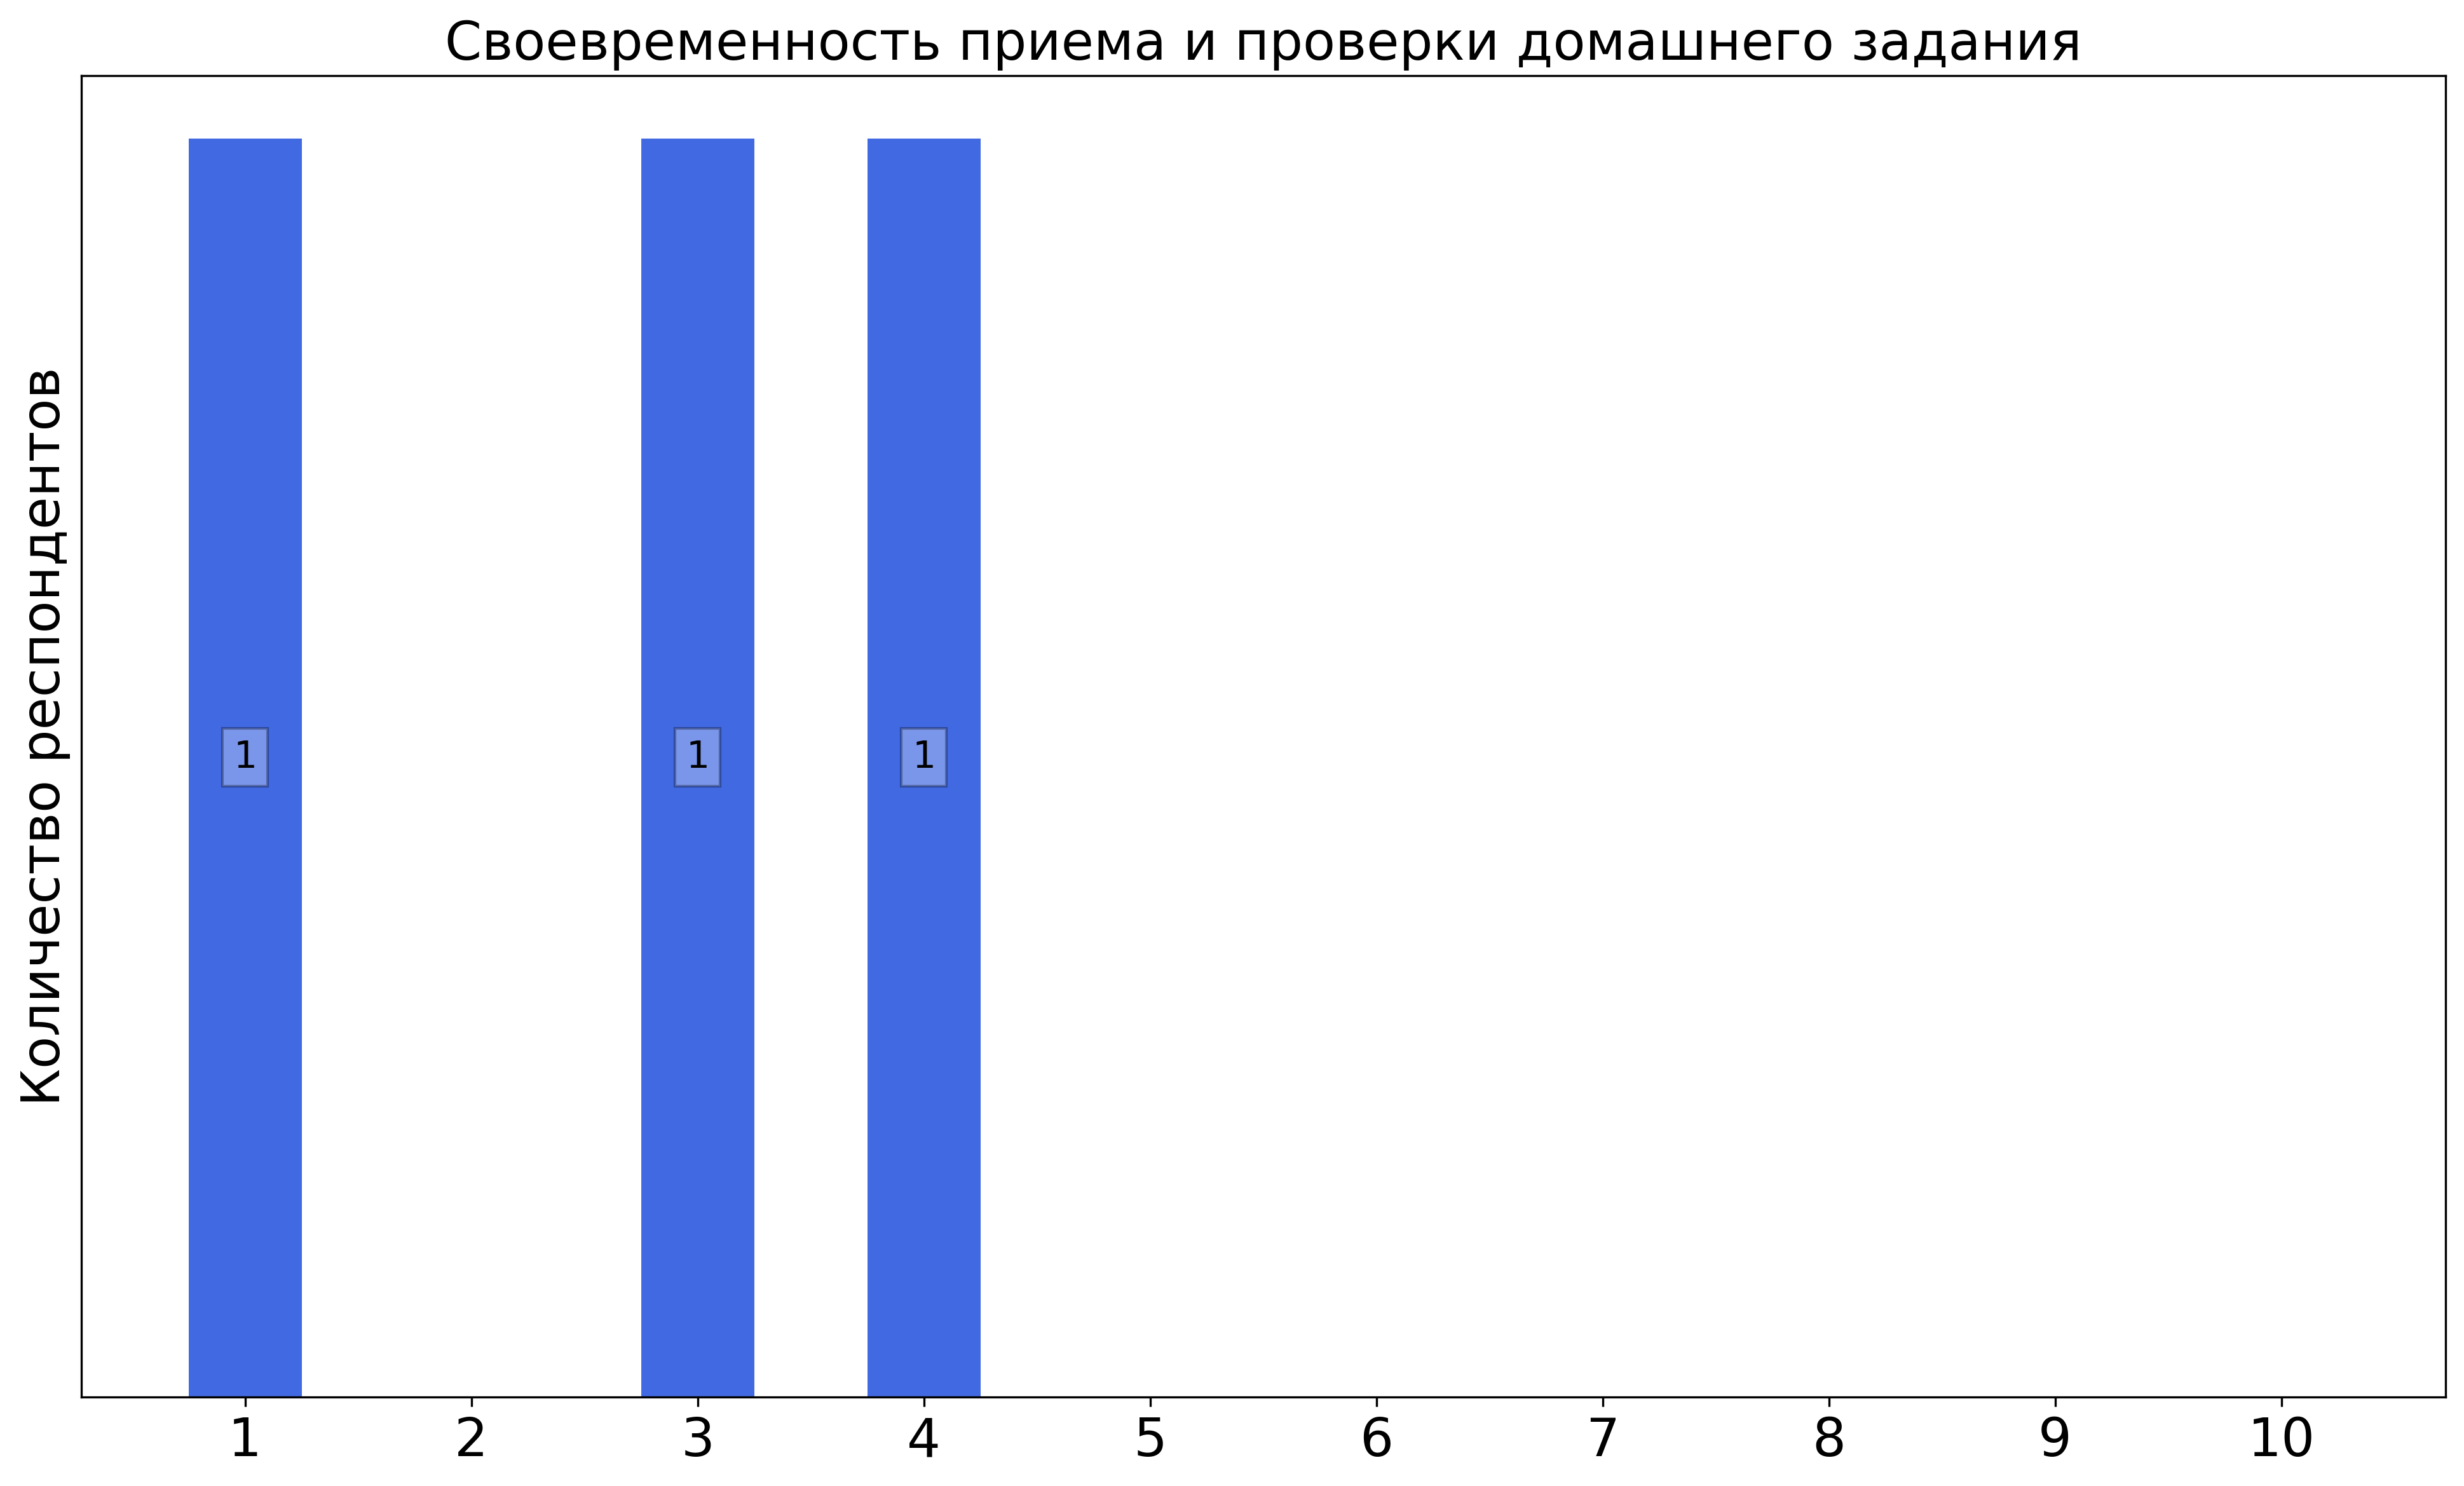
\includegraphics[width=\textwidth]{images/2 course/Общая физика - электричество и магнетизм/seminarists-marks-Долгих В.А.-2.png}
			\end{subfigure}
			\begin{subfigure}[b]{0.45\textwidth}
				\centering
				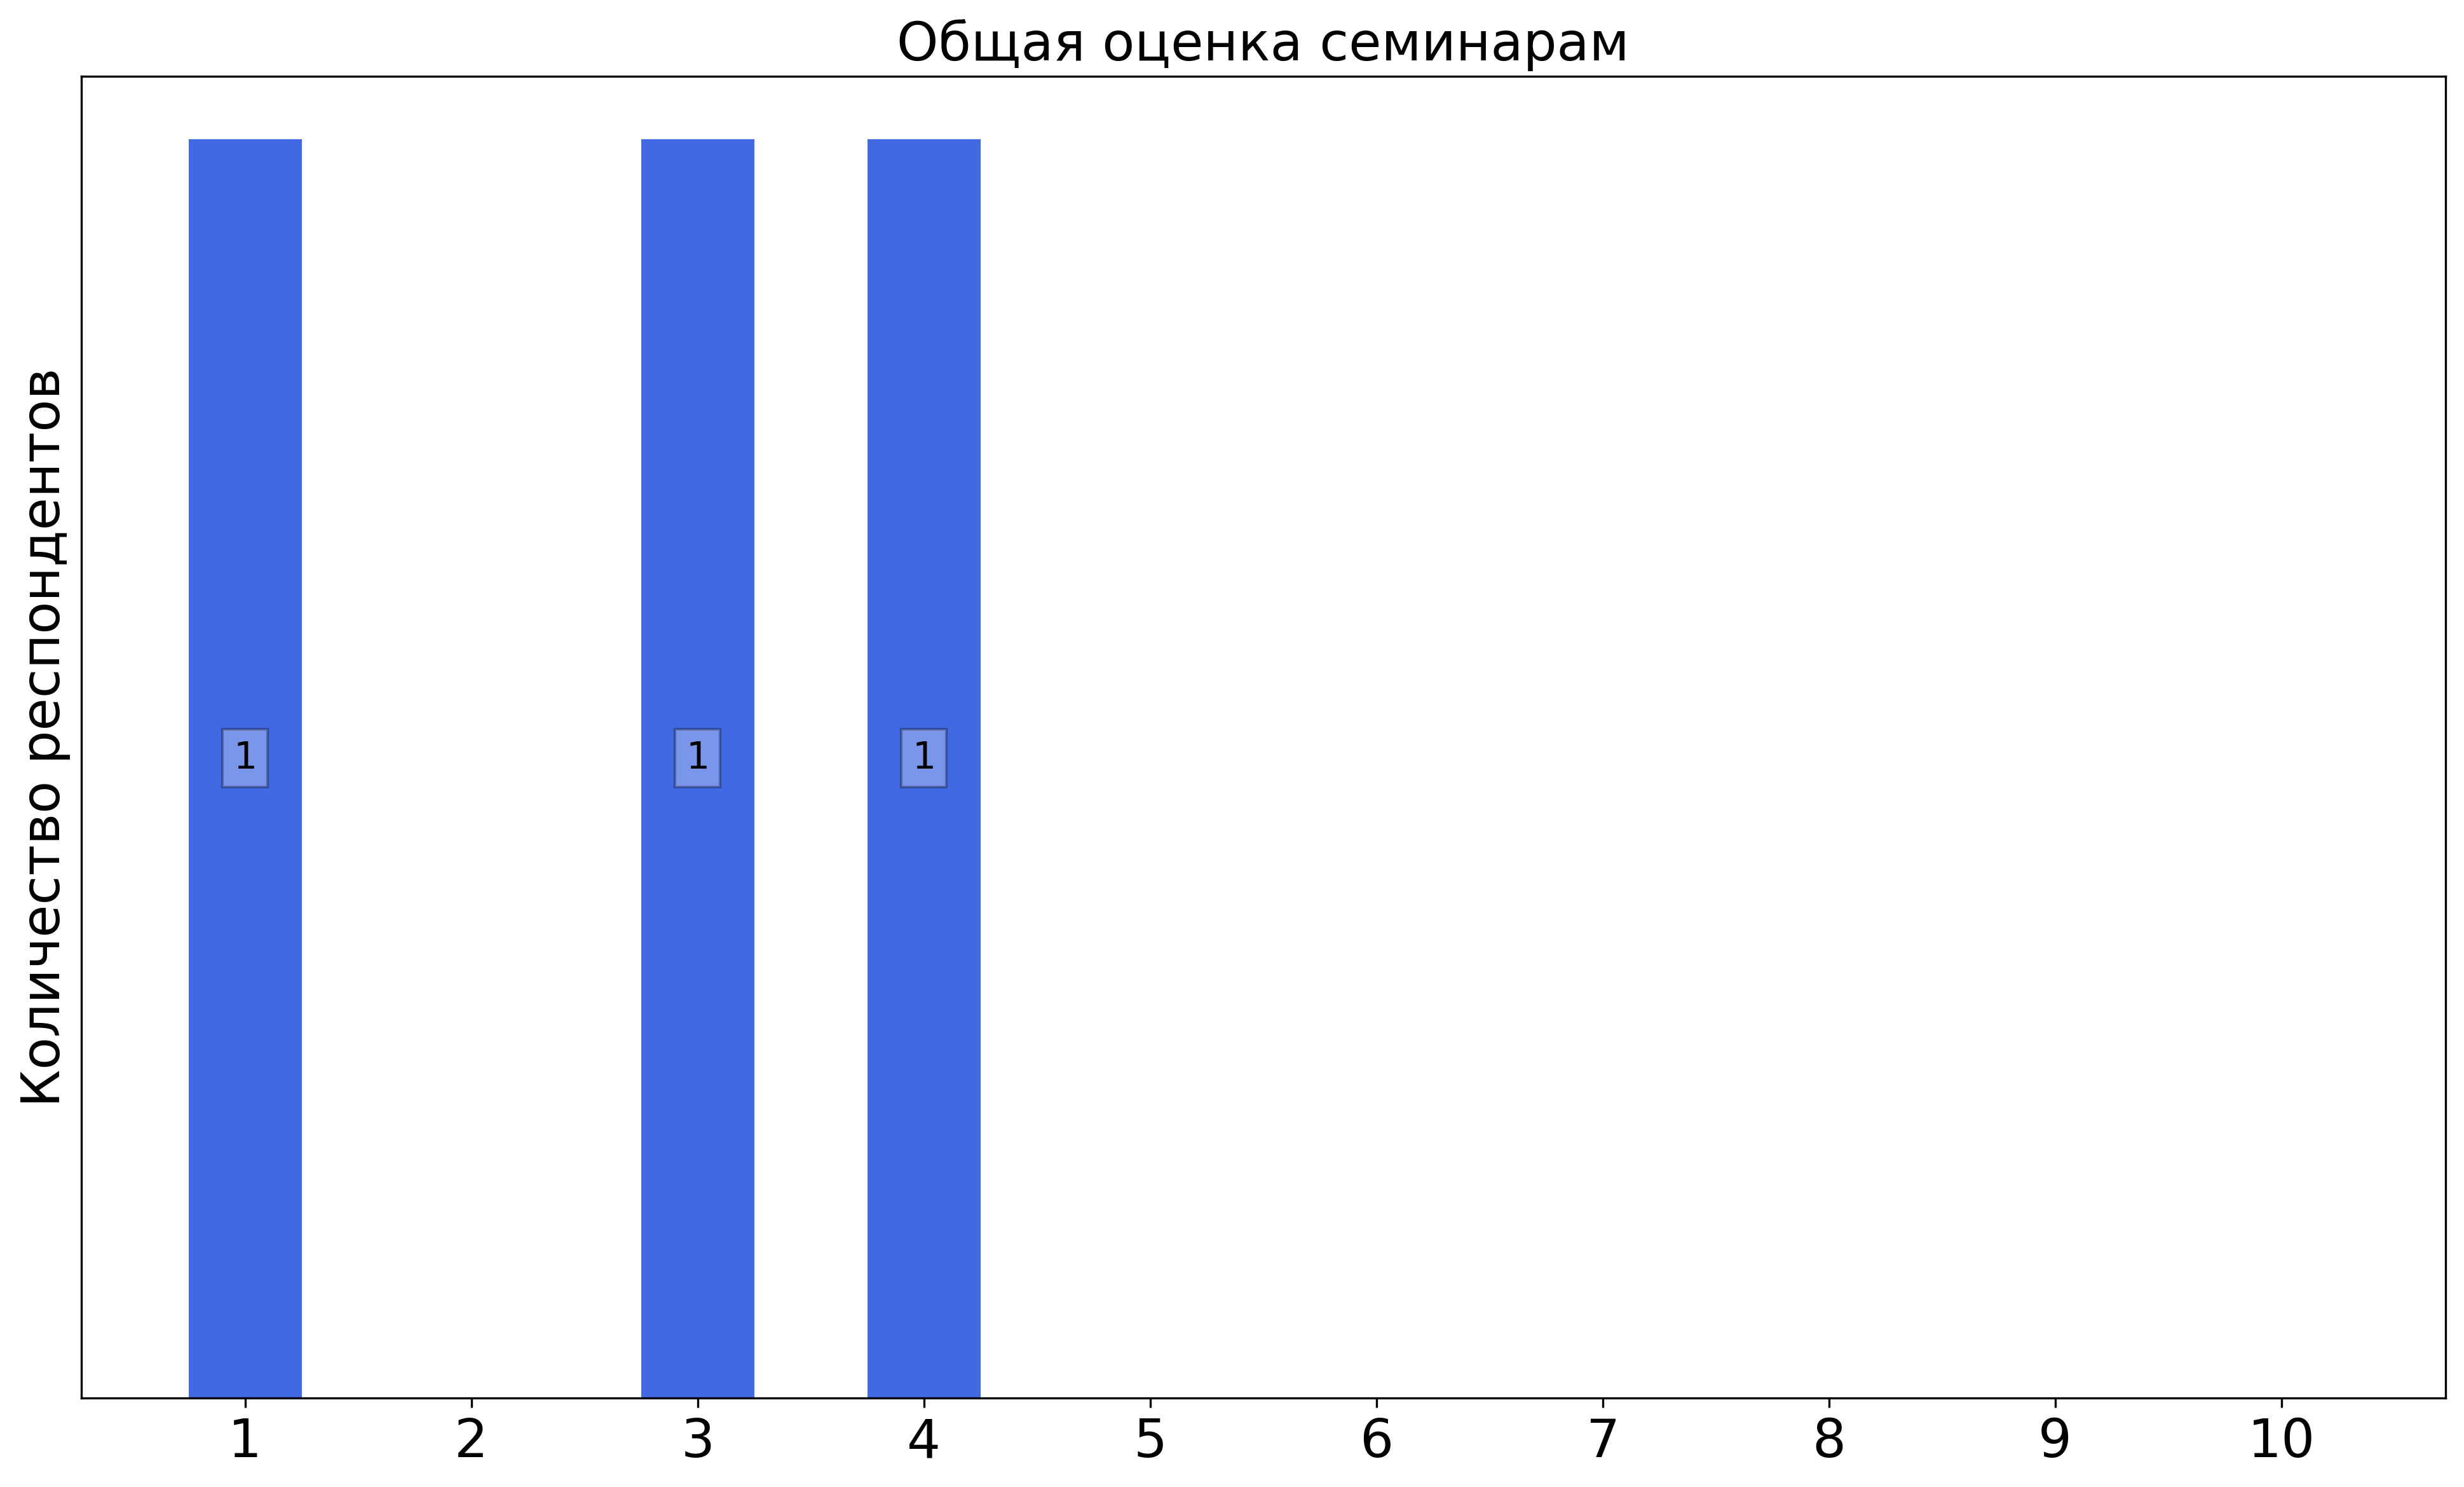
\includegraphics[width=\textwidth]{images/2 course/Общая физика - электричество и магнетизм/seminarists-marks-Долгих В.А.-3.png}
			\end{subfigure}	
			\caption{Оценки респондентов о качестве преподавания семинаров}
		\end{figure}

		\textbf{Комментарии студентов о семинаристе\protect\footnote{сохранены оригинальные орфография и пунктуация}}
			\begin{commentbox} 
				Долгих В.А. вёл у меня семинары по общей физике. Его семинары - это не семинары, а монотонное переписывание задач с доски в тетрадь. Да и для Долгих В.А. семинар это непрерывное переписывание задач с листочка на доску
				Долгих В.А. не объясняет теорию и не вдаётся в "физику" задачи. Семинары очень скучные и неинтересные, мотивации их посещать - нет. Я не смог научиться решать задачи по курсу общей физики, посетив каждый семинар Долгих В.А.
				Домашние задания Долгих В.А. скорее всего будет принимать у всей группы сразу и эта сдача превратится в экзистенциальный ужас. 
				Долгих В.А., однако, действительно переживает за студентов на экзамене и всячески старается помочь своей группе, но я полагаю, этого мало, чтобы назвать его хорошим преподавателем.
				Общаться с Долгих В.А. крайне тяжело 
			\end{commentbox}


	\subsubsection{Отзыв студентов о семинарах. Семинарист: Крымский К.М.}
		\begin{figure}[H]
			\centering
			\begin{subfigure}[b]{0.45\textwidth}
				\centering
				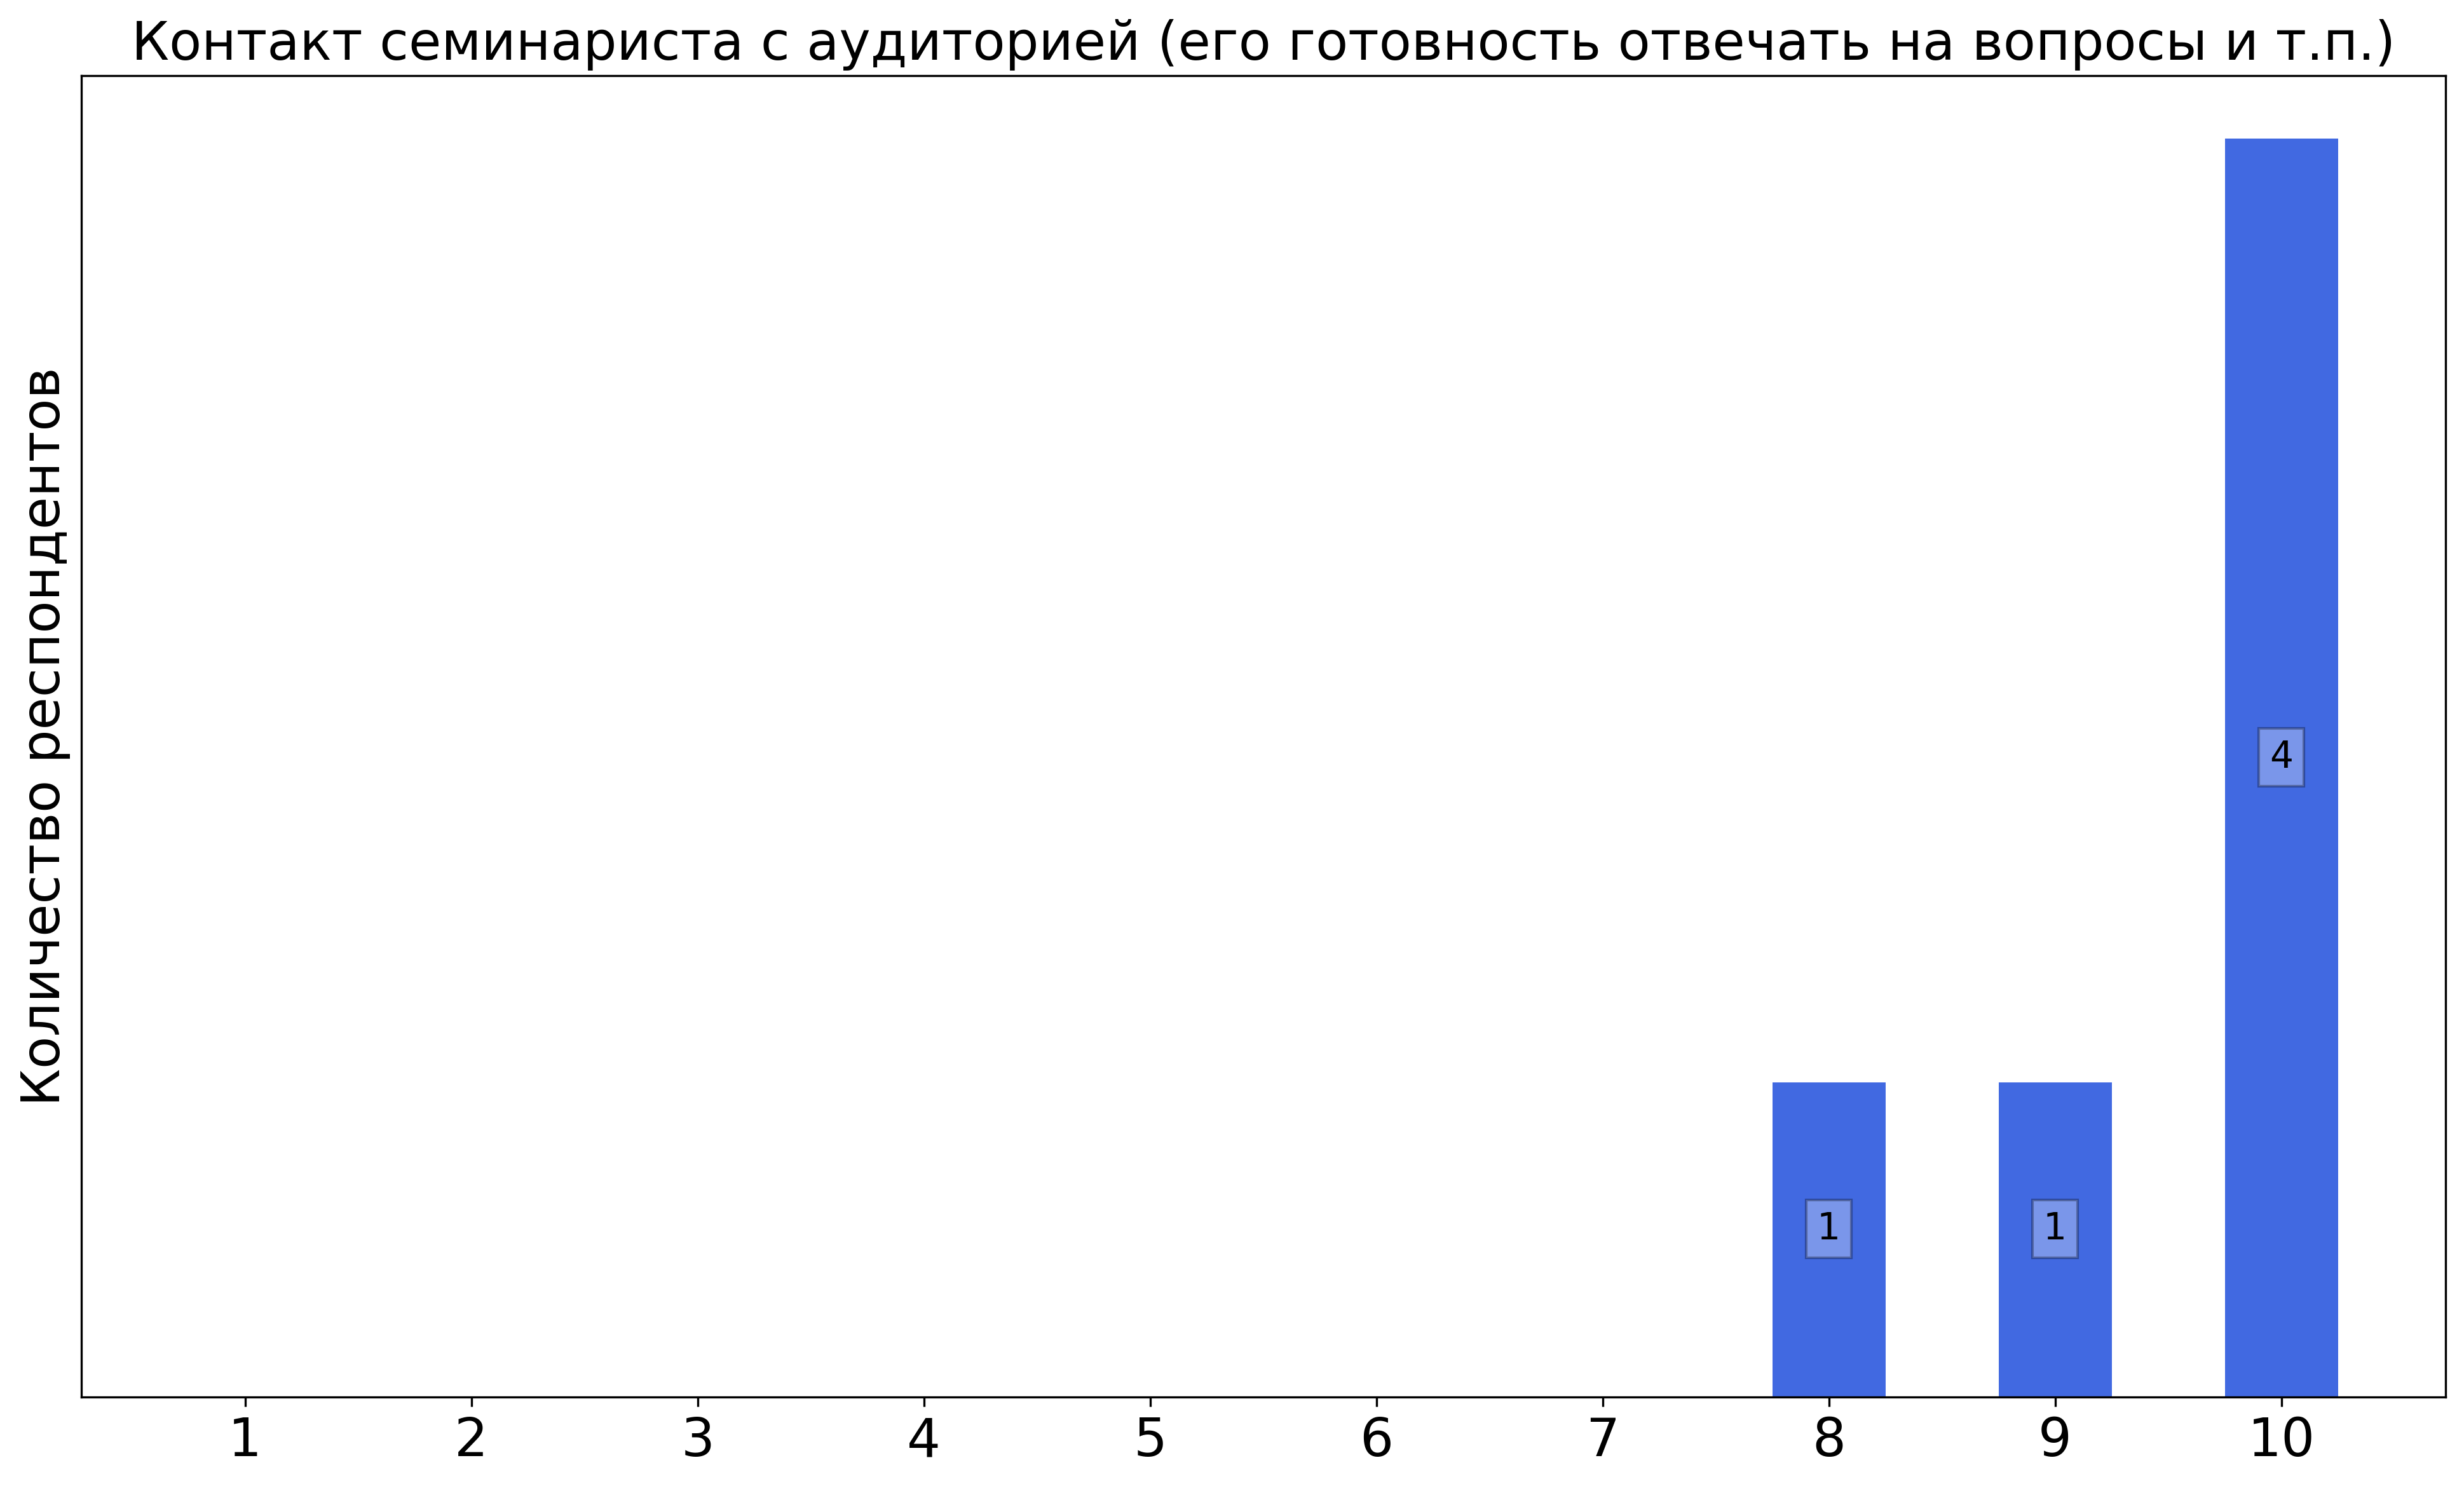
\includegraphics[width=\textwidth]{images/2 course/Общая физика - электричество и магнетизм/seminarists-marks-Крымский К.М.-0.png}
			\end{subfigure}
			\begin{subfigure}[b]{0.45\textwidth}
				\centering
				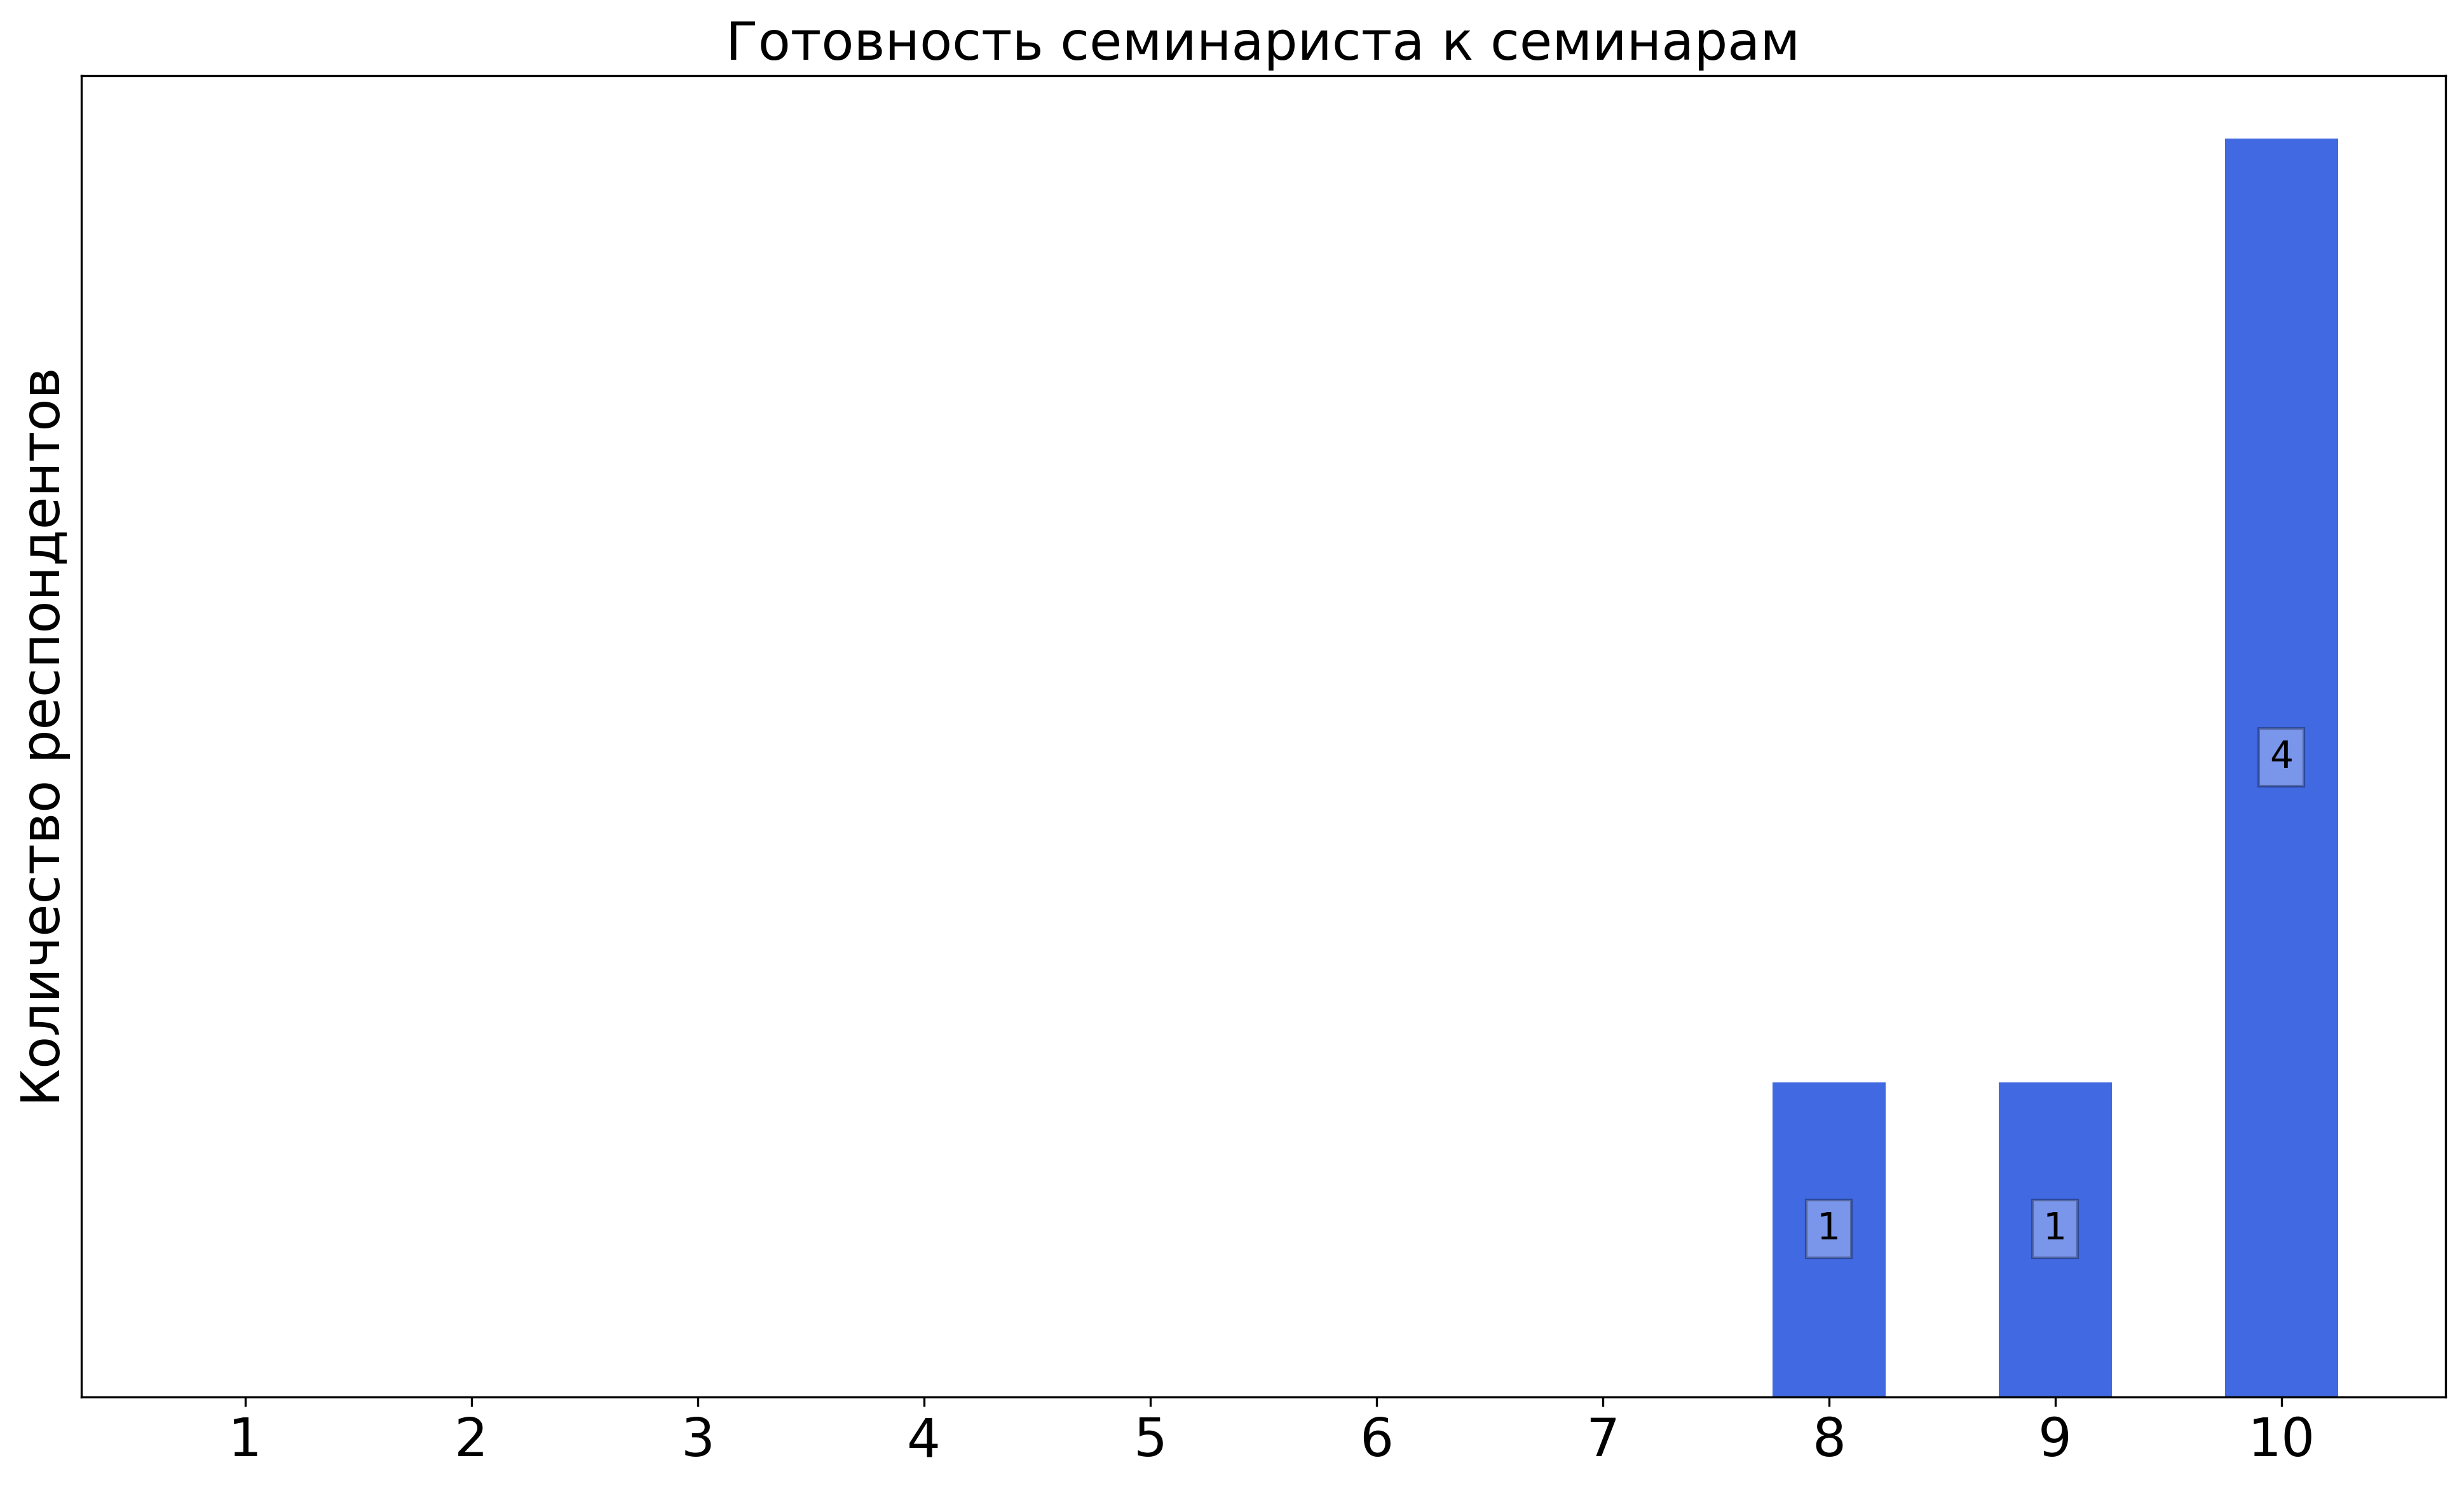
\includegraphics[width=\textwidth]{images/2 course/Общая физика - электричество и магнетизм/seminarists-marks-Крымский К.М.-1.png}
			\end{subfigure}
			\begin{subfigure}[b]{0.45\textwidth}
				\centering
				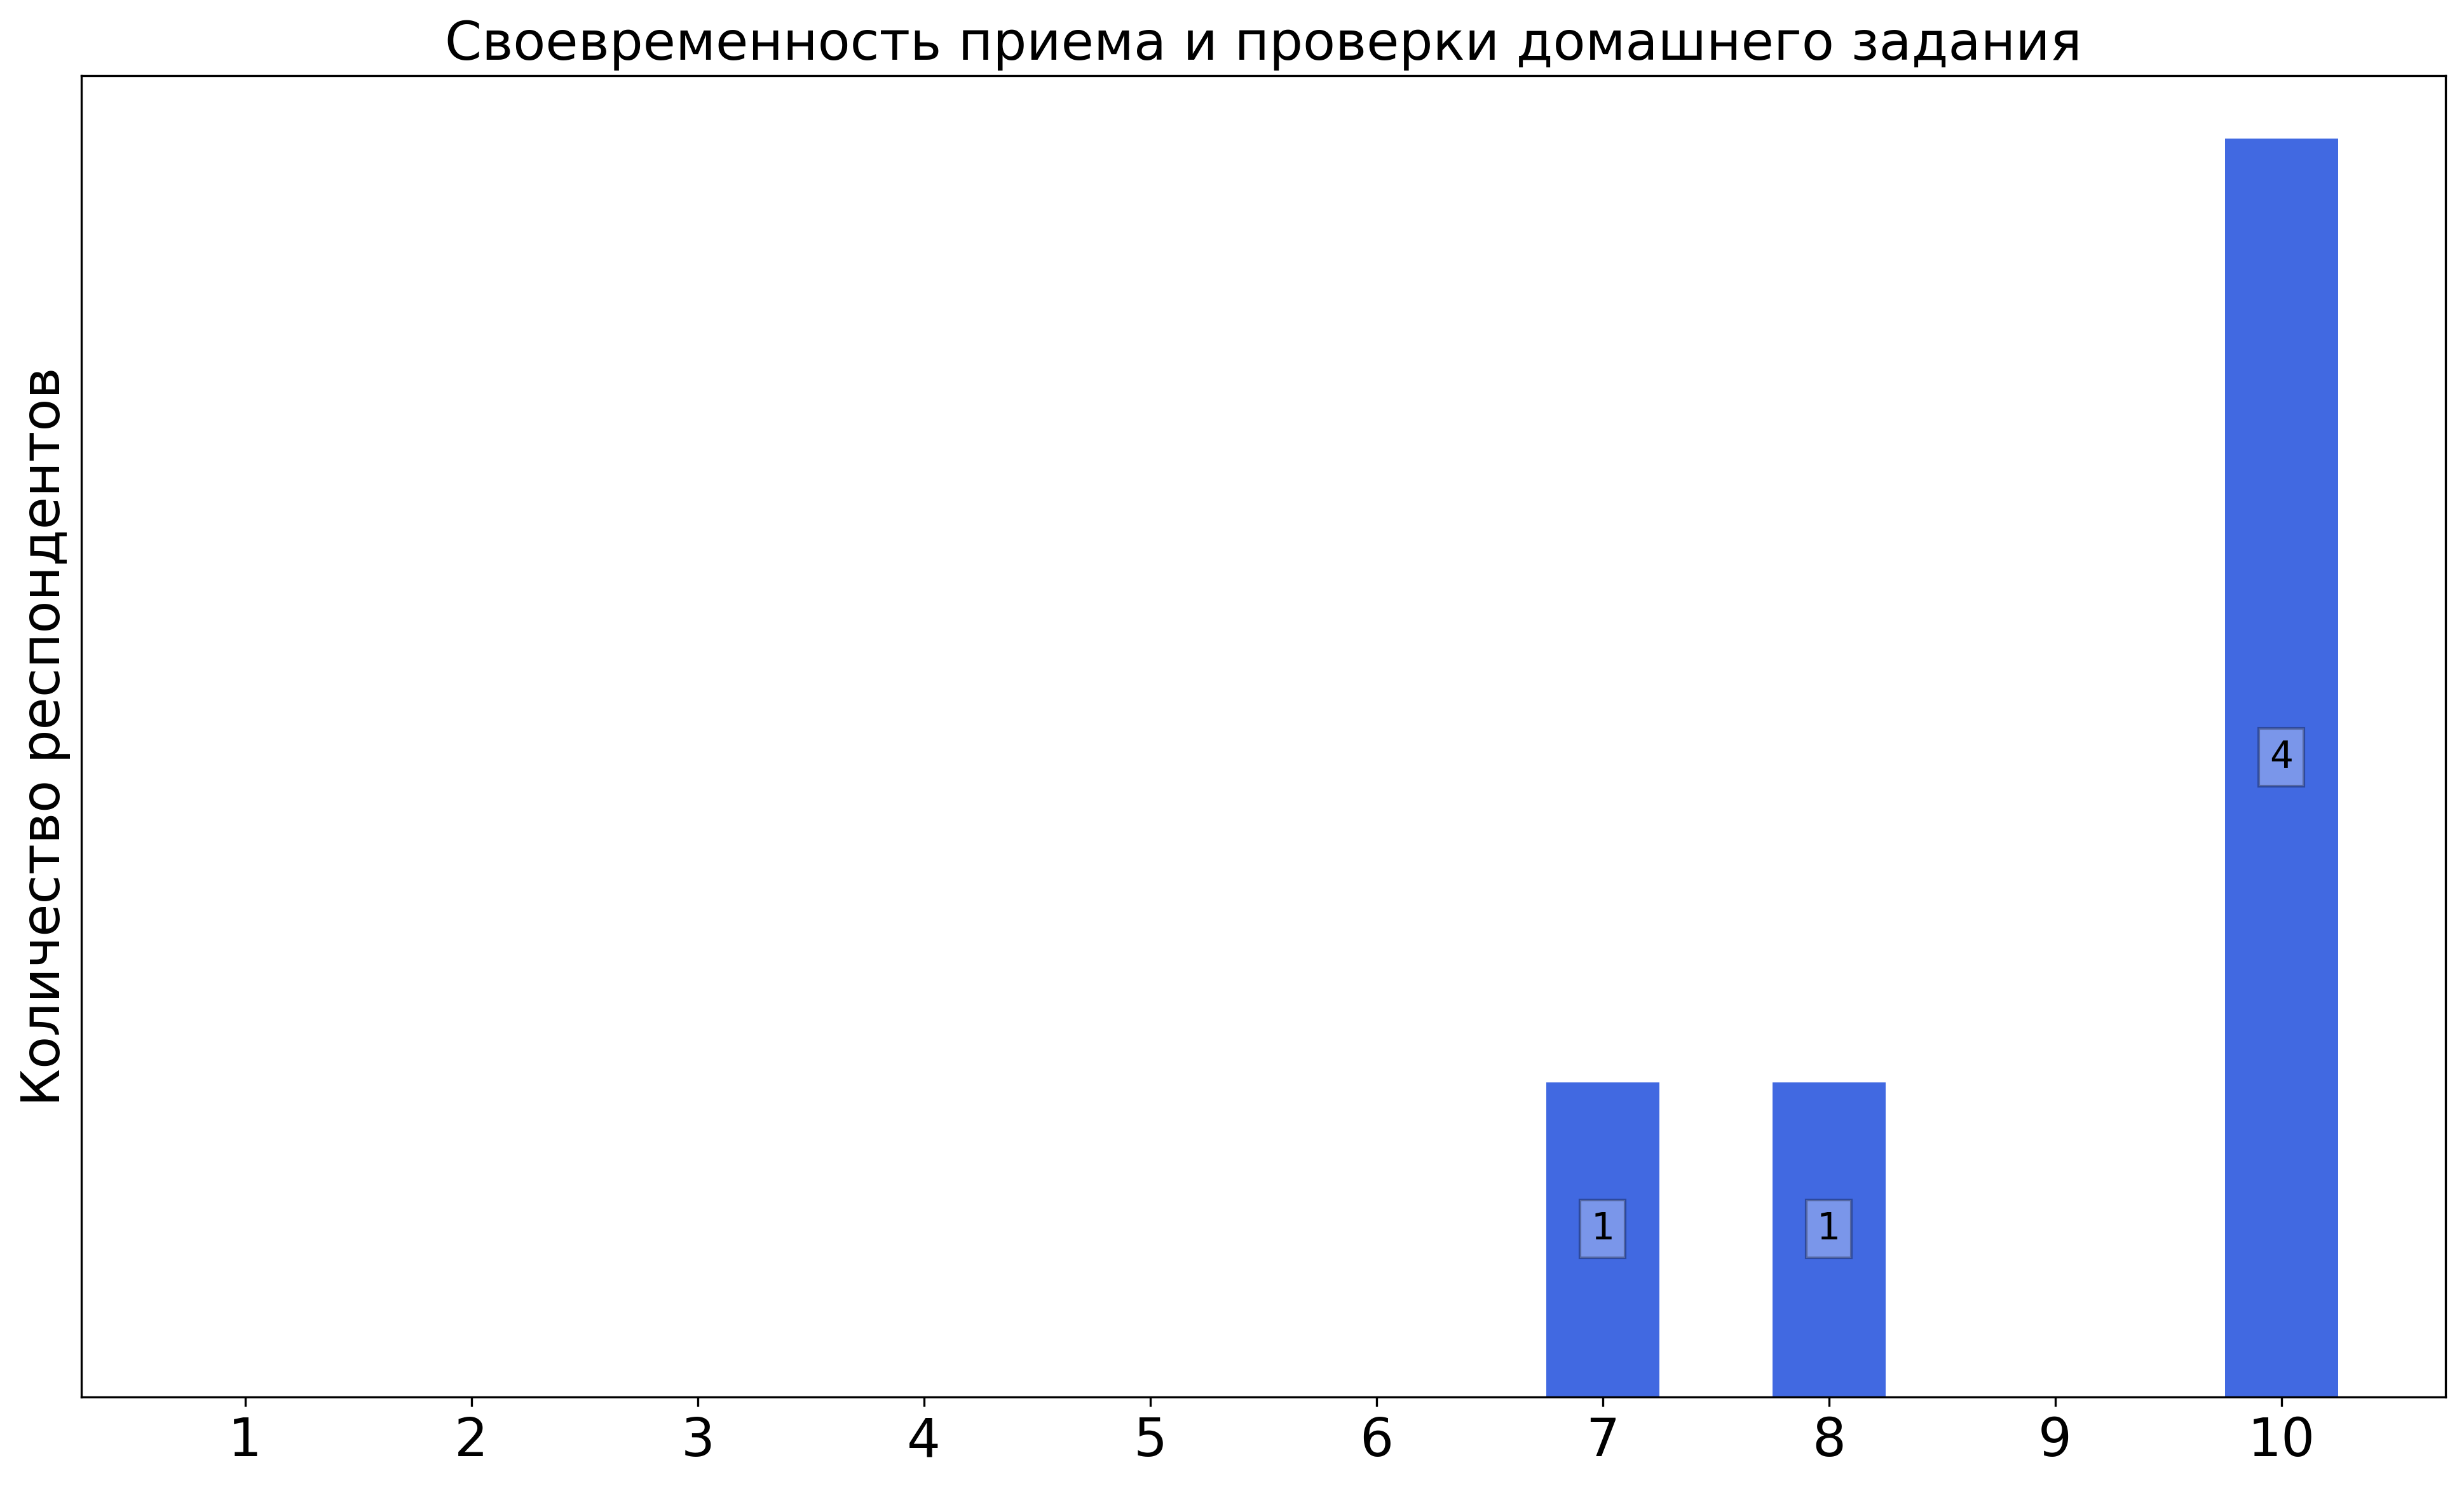
\includegraphics[width=\textwidth]{images/2 course/Общая физика - электричество и магнетизм/seminarists-marks-Крымский К.М.-2.png}
			\end{subfigure}
			\begin{subfigure}[b]{0.45\textwidth}
				\centering
				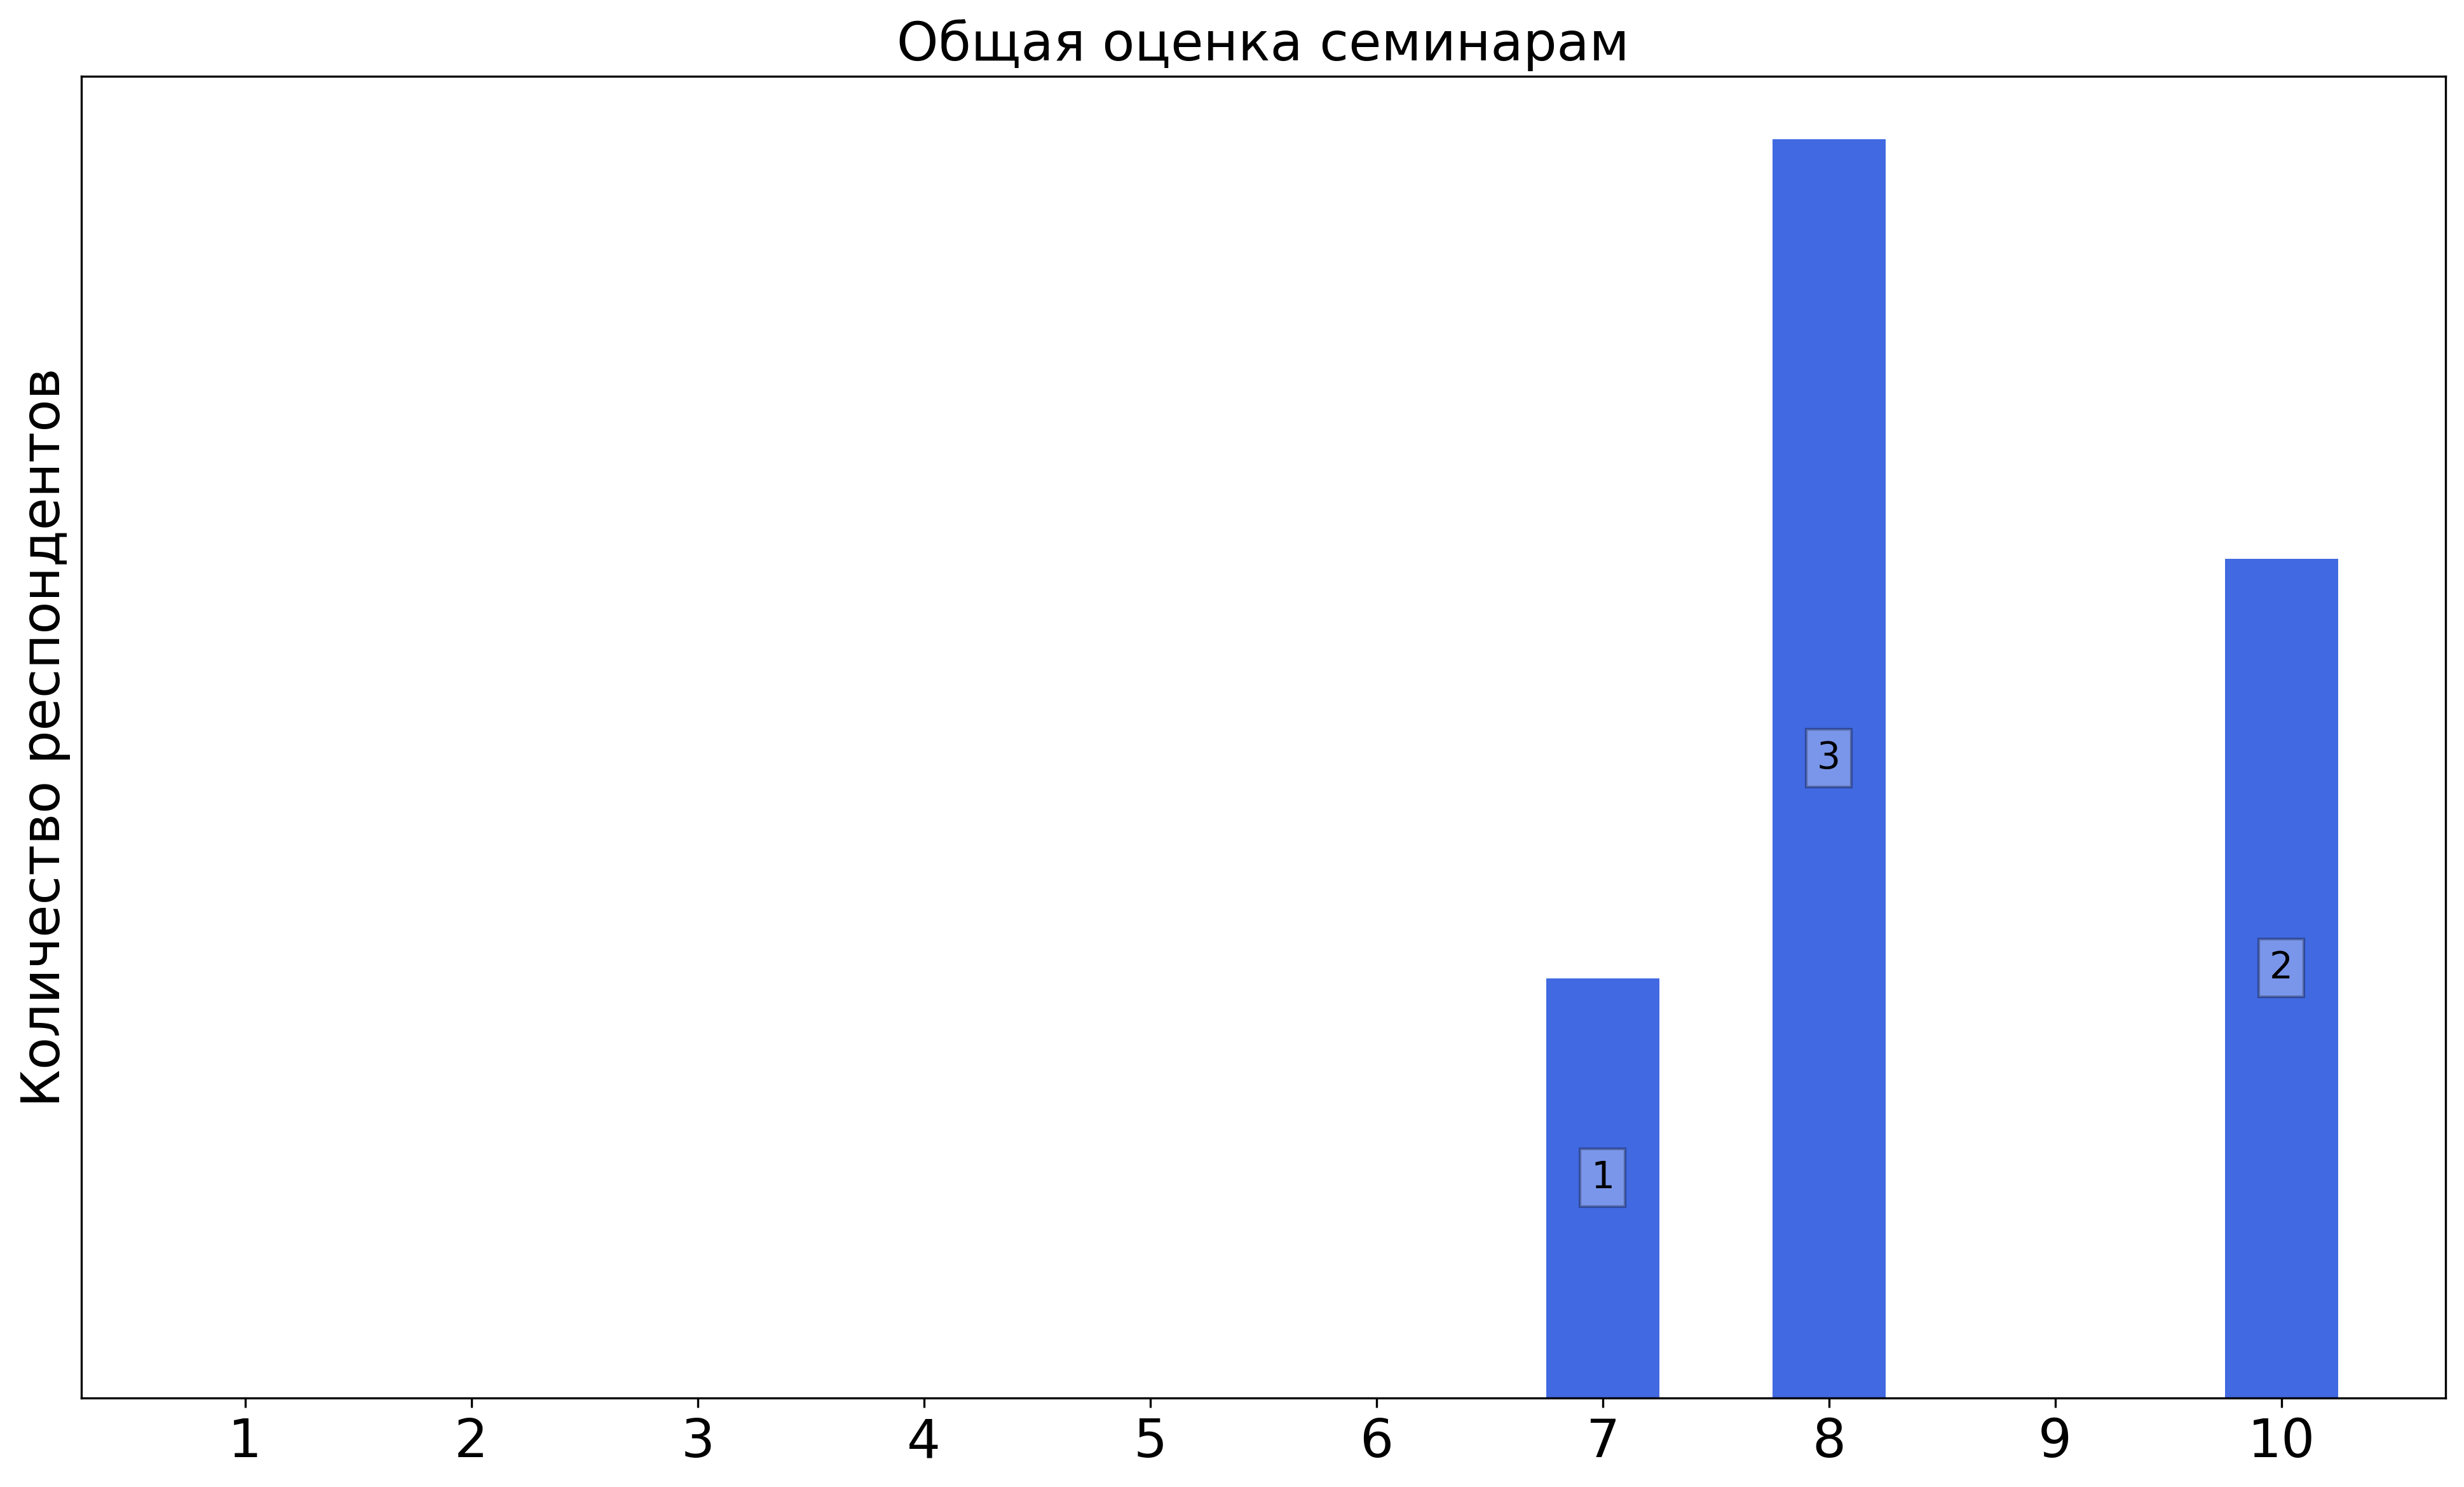
\includegraphics[width=\textwidth]{images/2 course/Общая физика - электричество и магнетизм/seminarists-marks-Крымский К.М.-3.png}
			\end{subfigure}	
			\caption{Оценки респондентов о качестве преподавания семинаров}
		\end{figure}
		
		
	\subsubsection{Отзыв студентов о семинарах. Семинарист: Максимычев А.В.}
		\begin{figure}[H]
			\centering
			\begin{subfigure}[b]{0.45\textwidth}
				\centering
				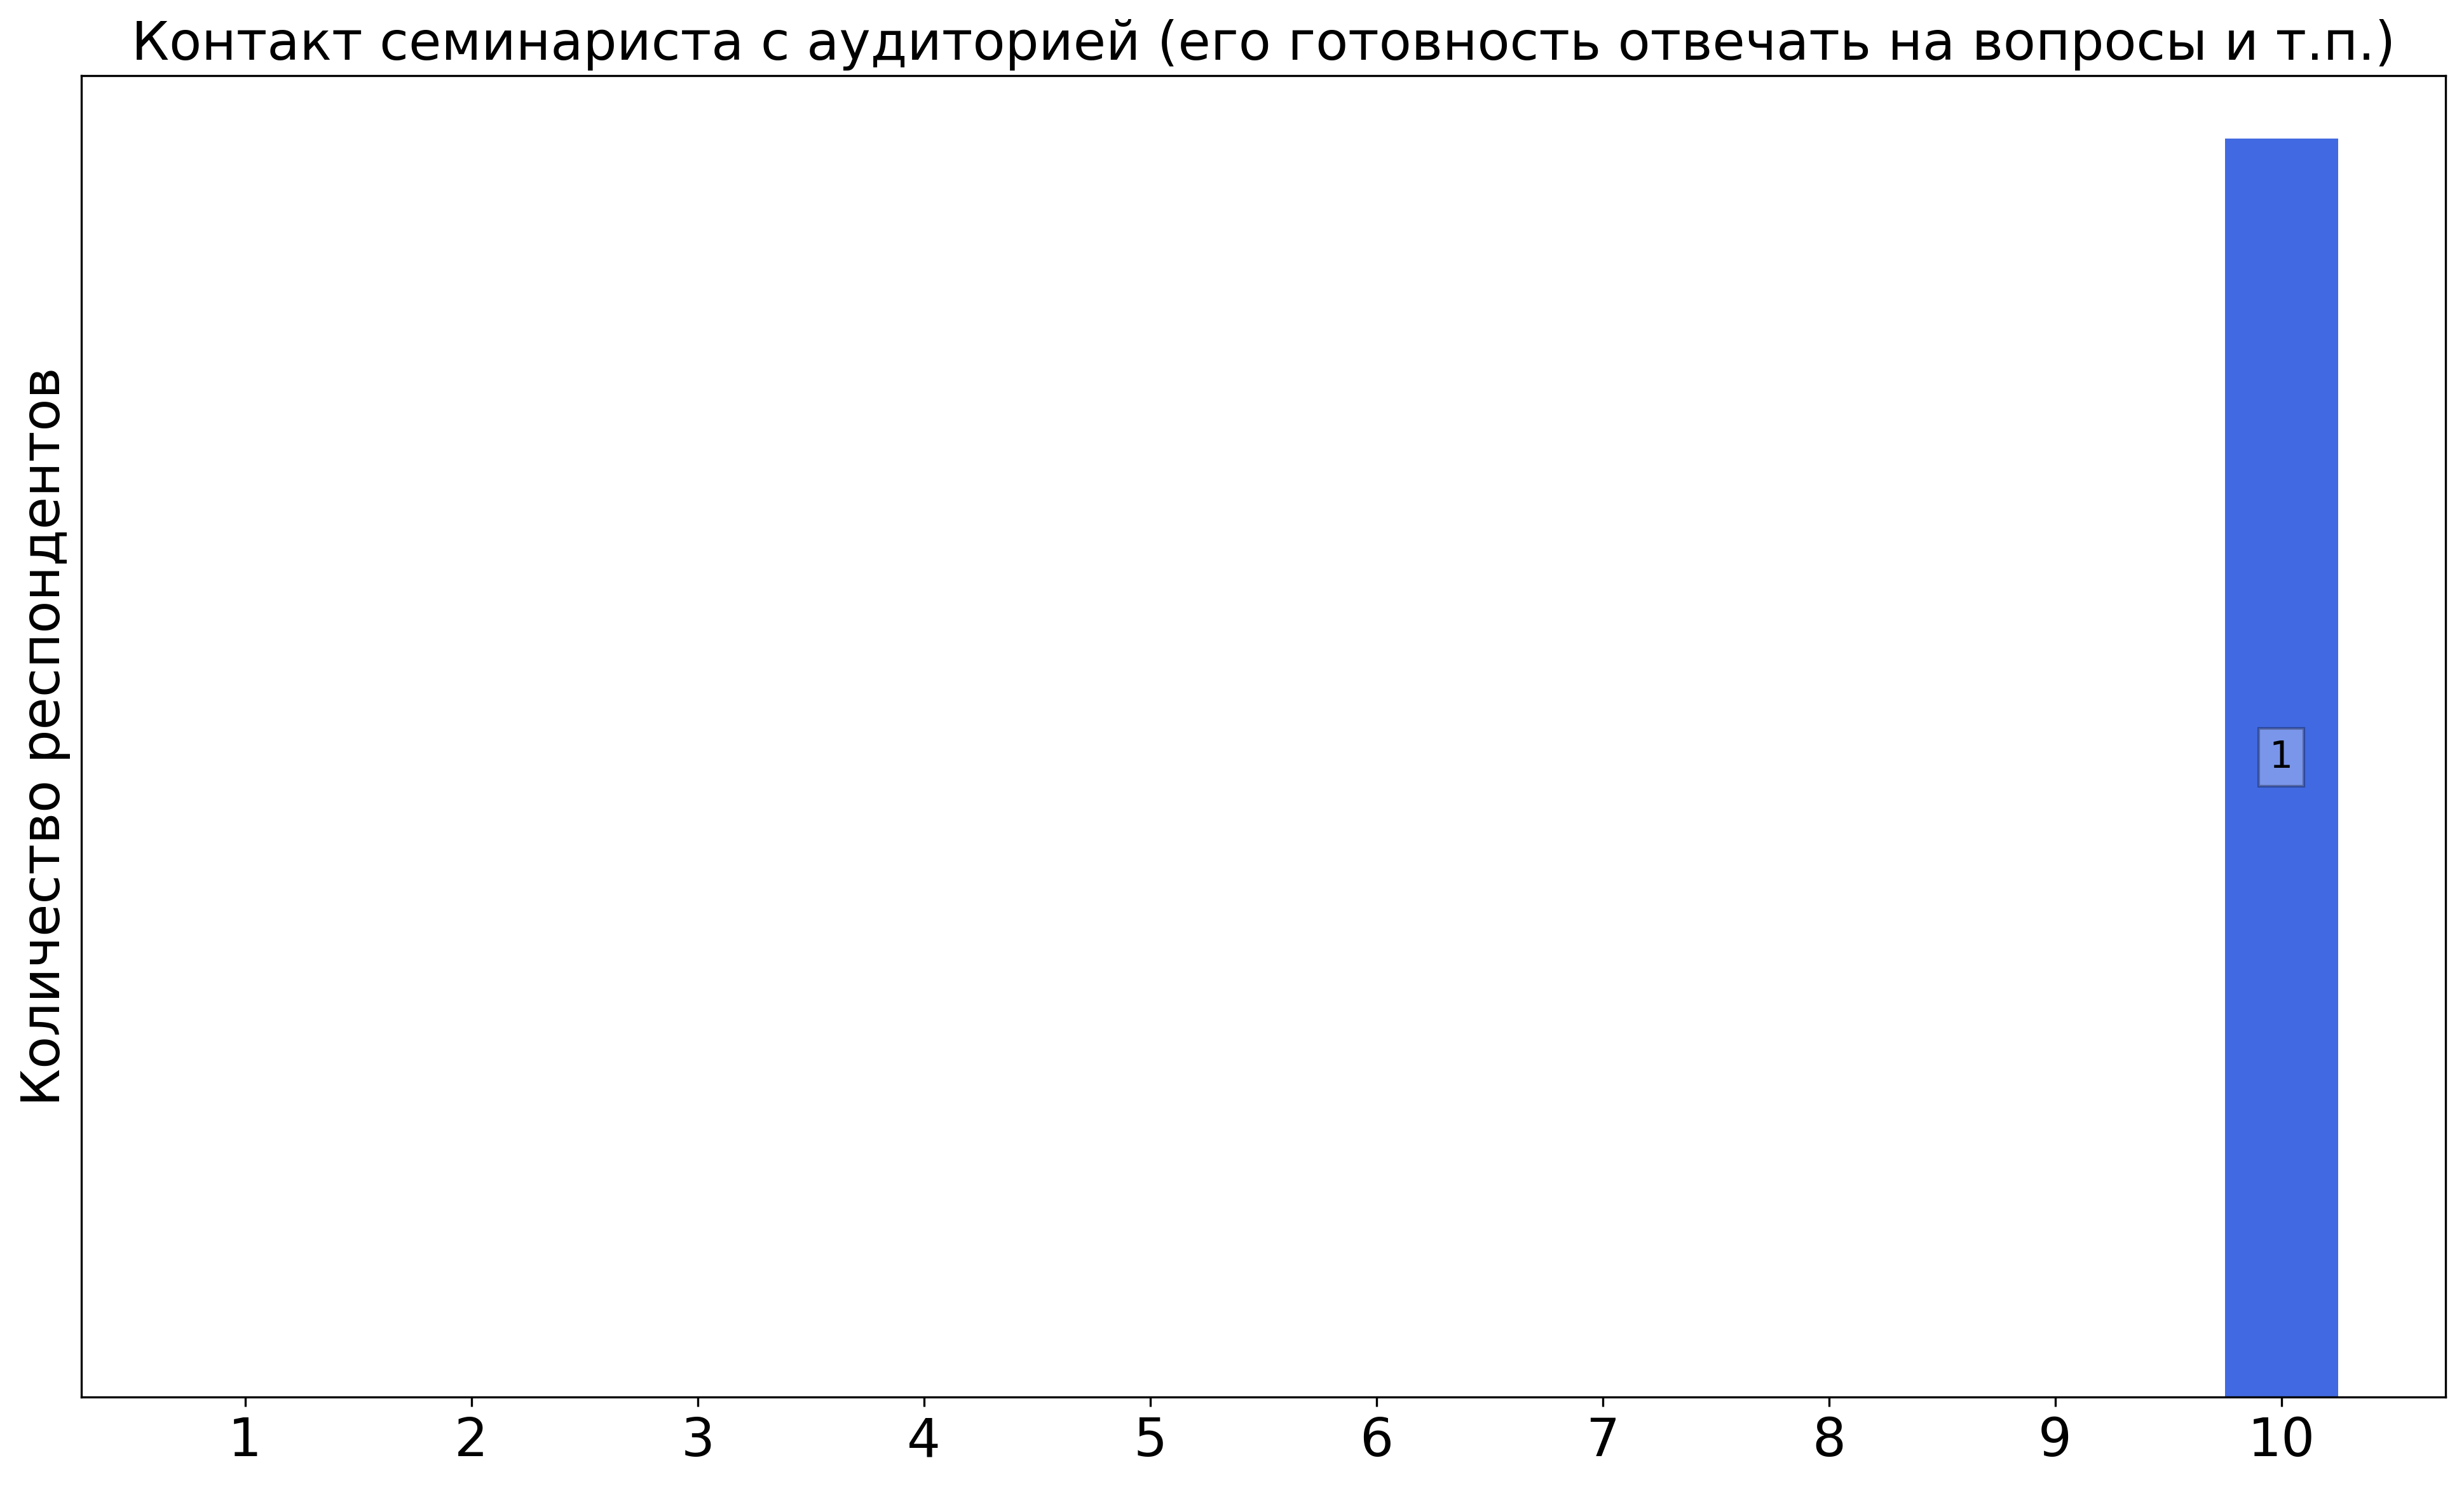
\includegraphics[width=\textwidth]{images/2 course/Общая физика - электричество и магнетизм/seminarists-marks-Максимычев А.В.-0.png}
			\end{subfigure}
			\begin{subfigure}[b]{0.45\textwidth}
				\centering
				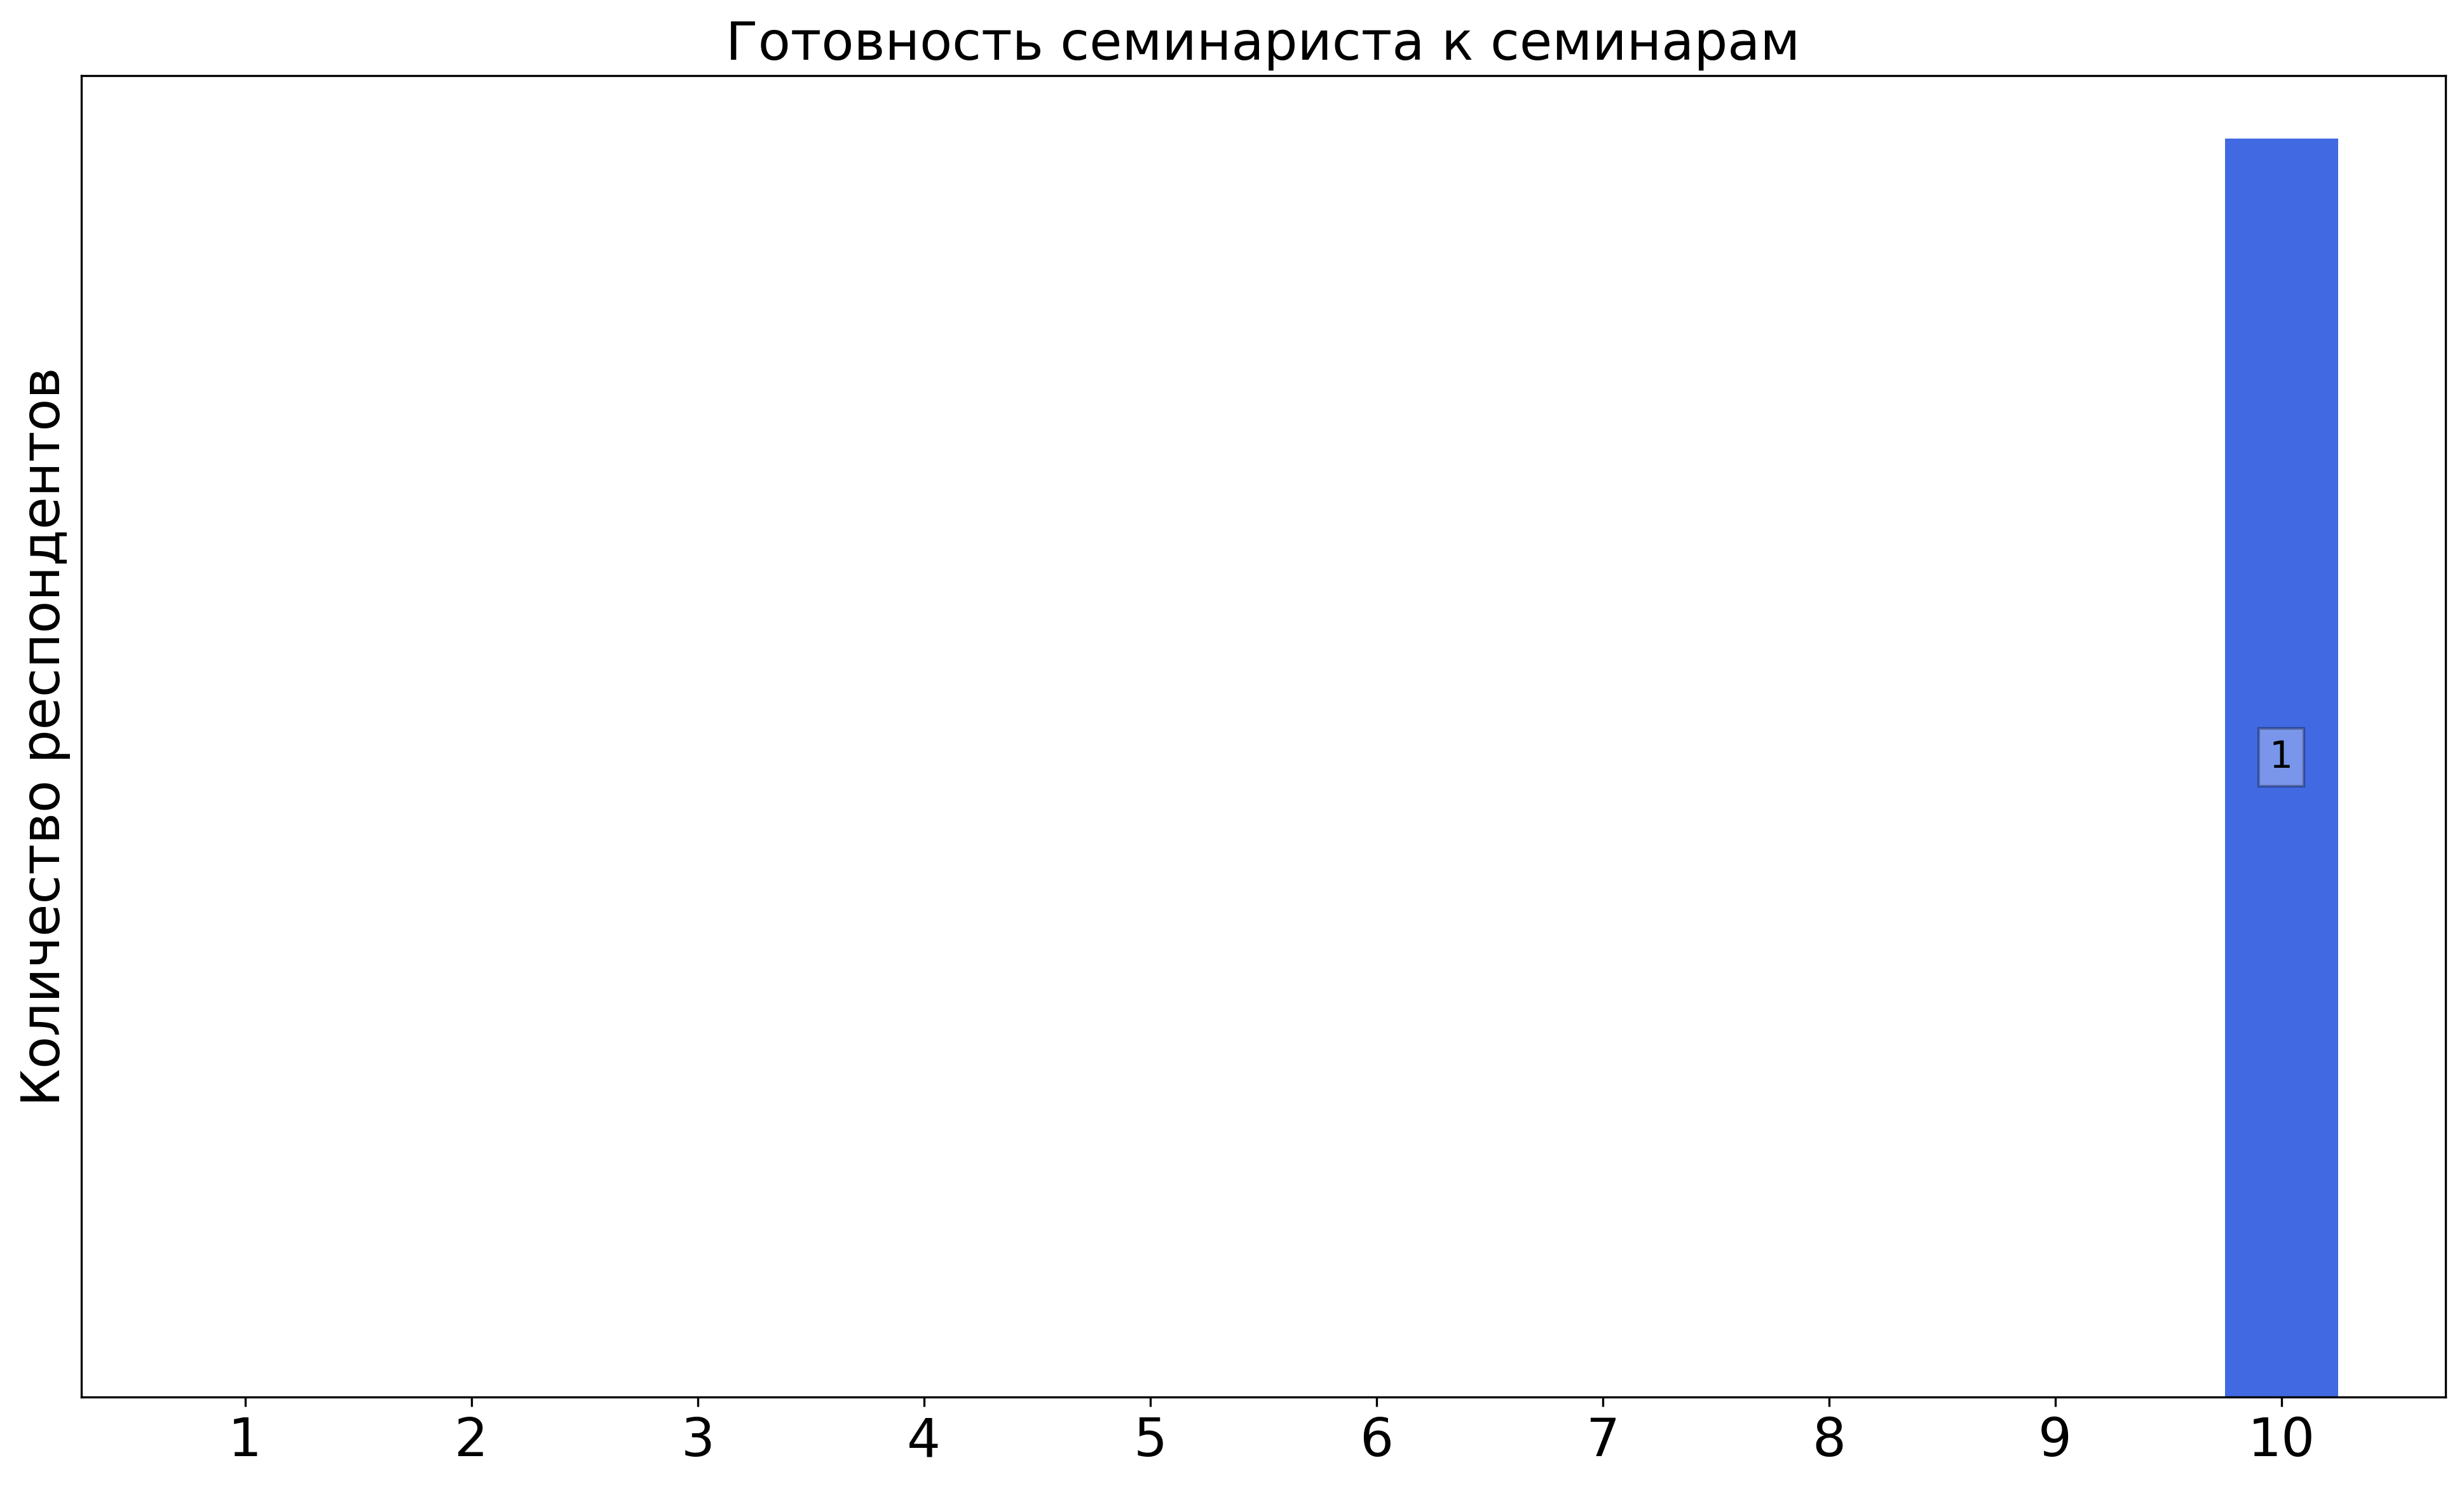
\includegraphics[width=\textwidth]{images/2 course/Общая физика - электричество и магнетизм/seminarists-marks-Максимычев А.В.-1.png}
			\end{subfigure}
			\begin{subfigure}[b]{0.45\textwidth}
				\centering
				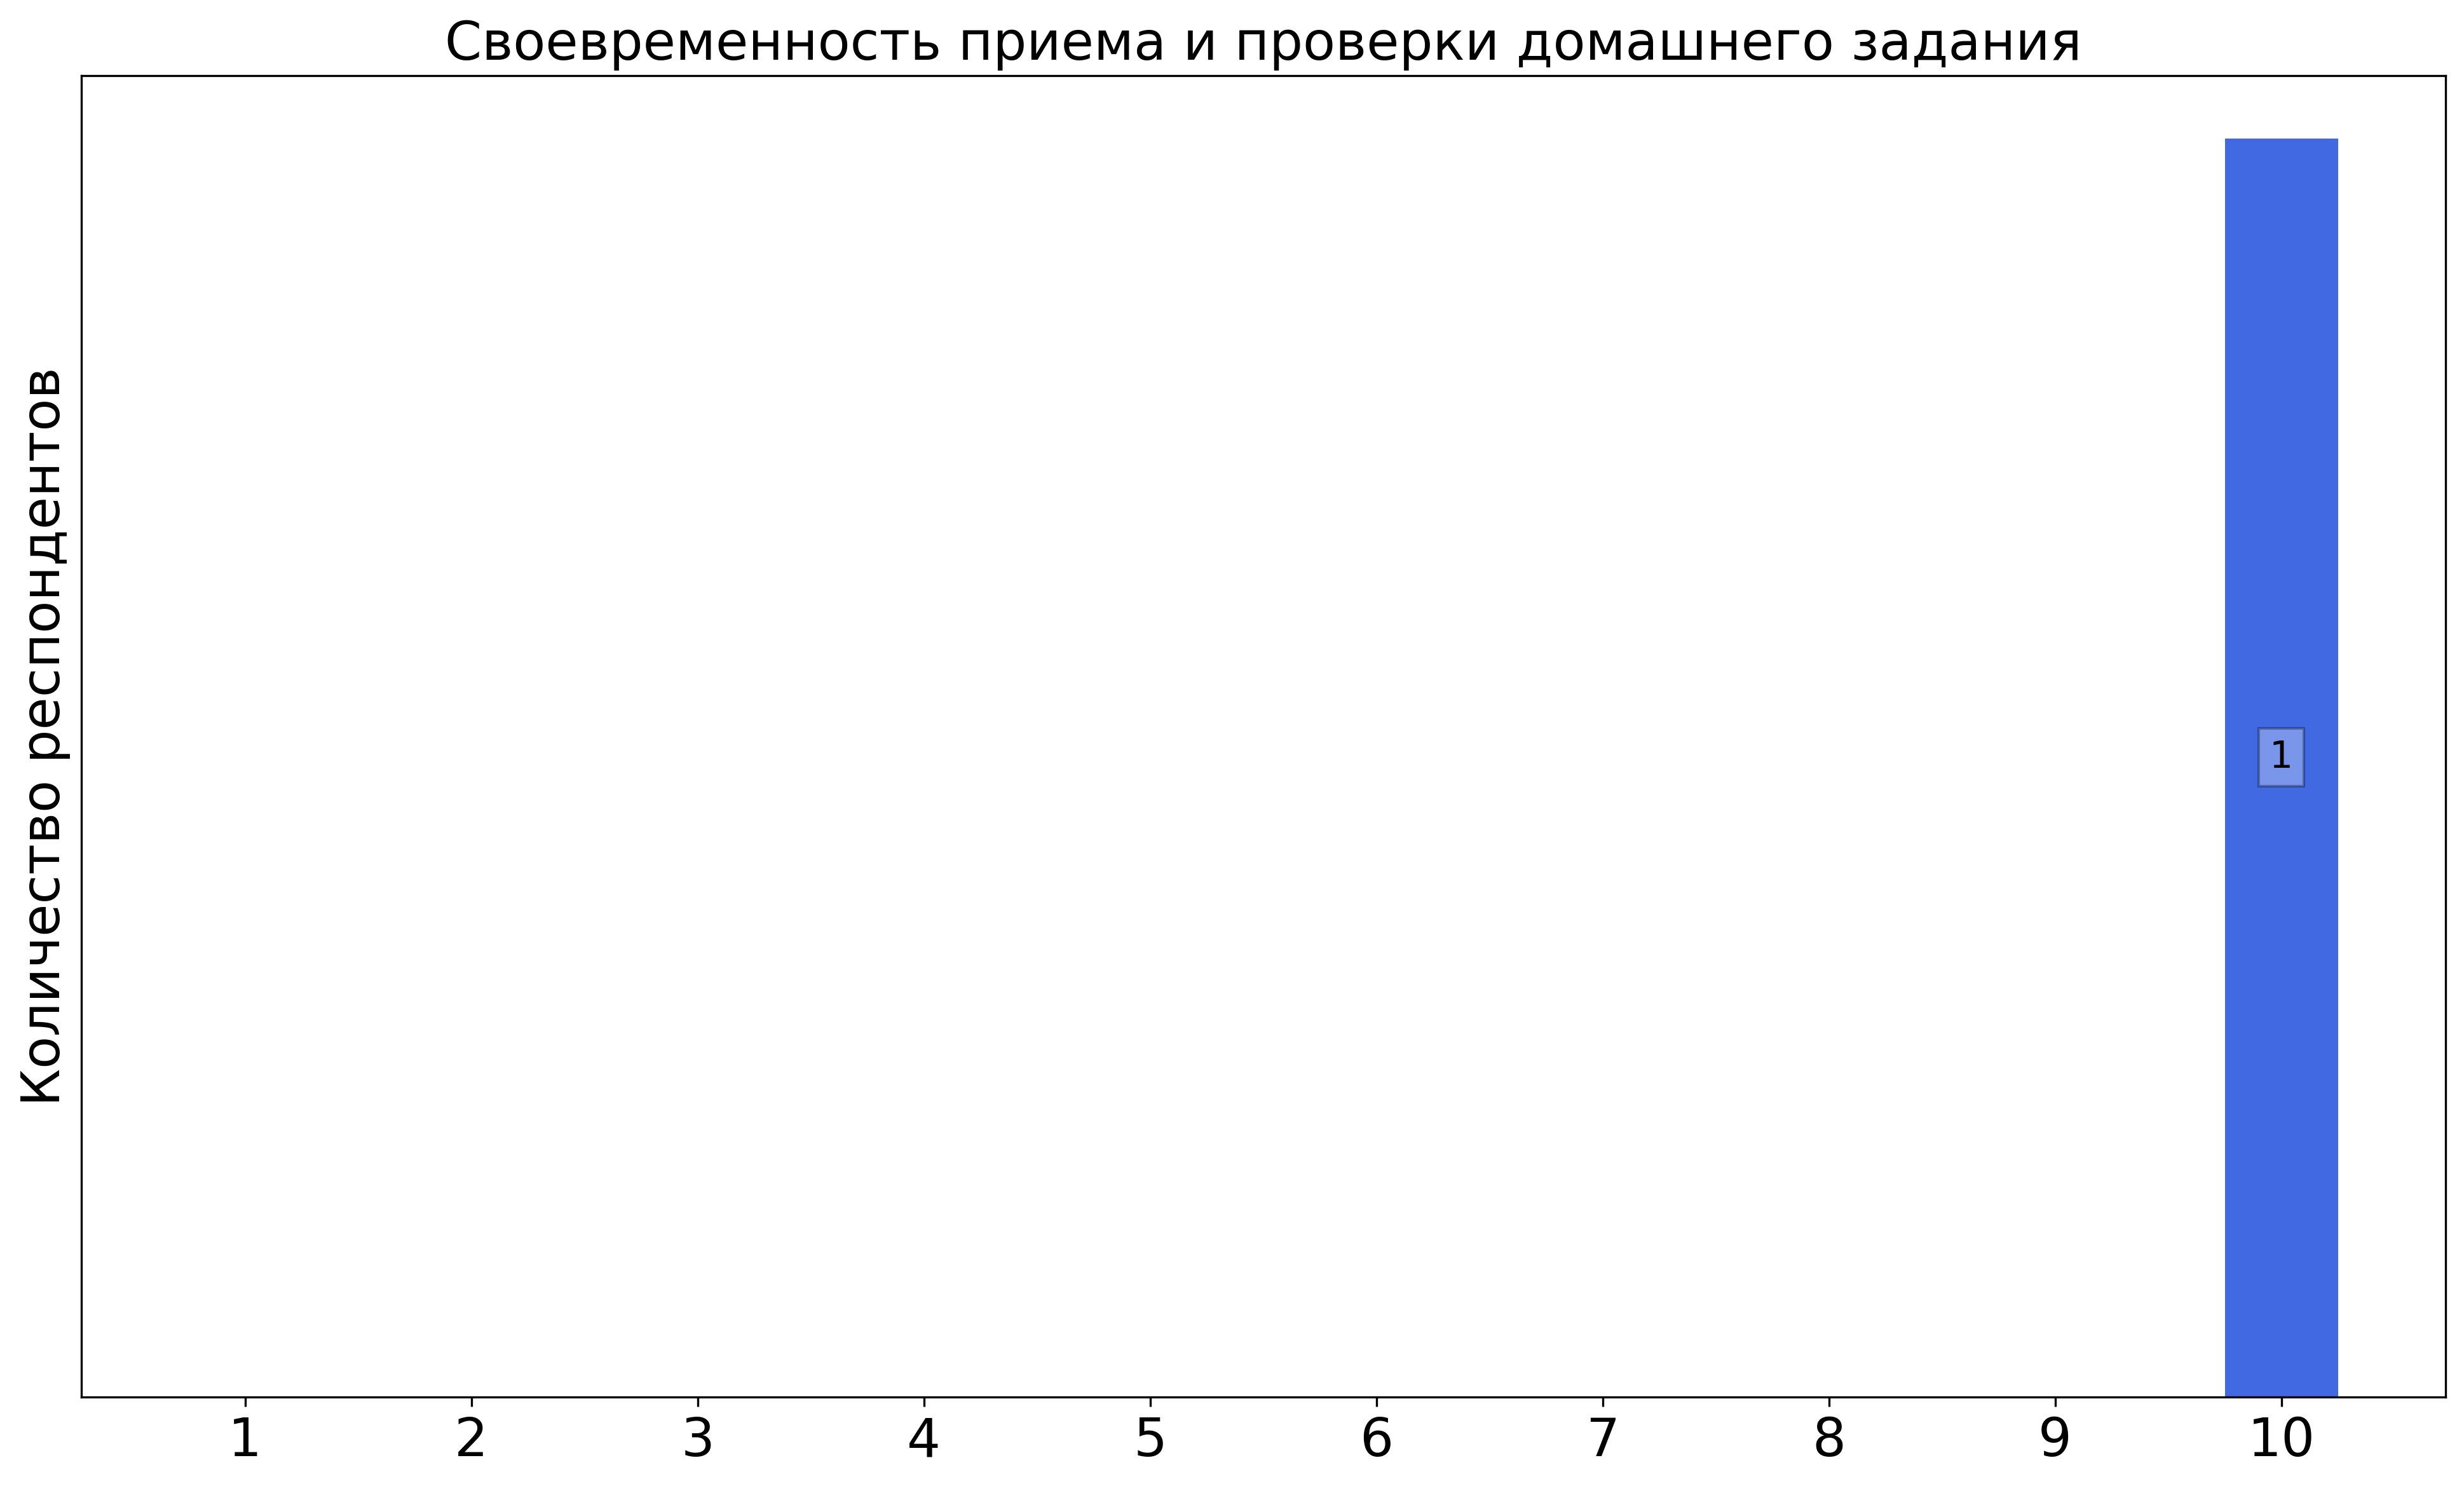
\includegraphics[width=\textwidth]{images/2 course/Общая физика - электричество и магнетизм/seminarists-marks-Максимычев А.В.-2.png}
			\end{subfigure}
			\begin{subfigure}[b]{0.45\textwidth}
				\centering
				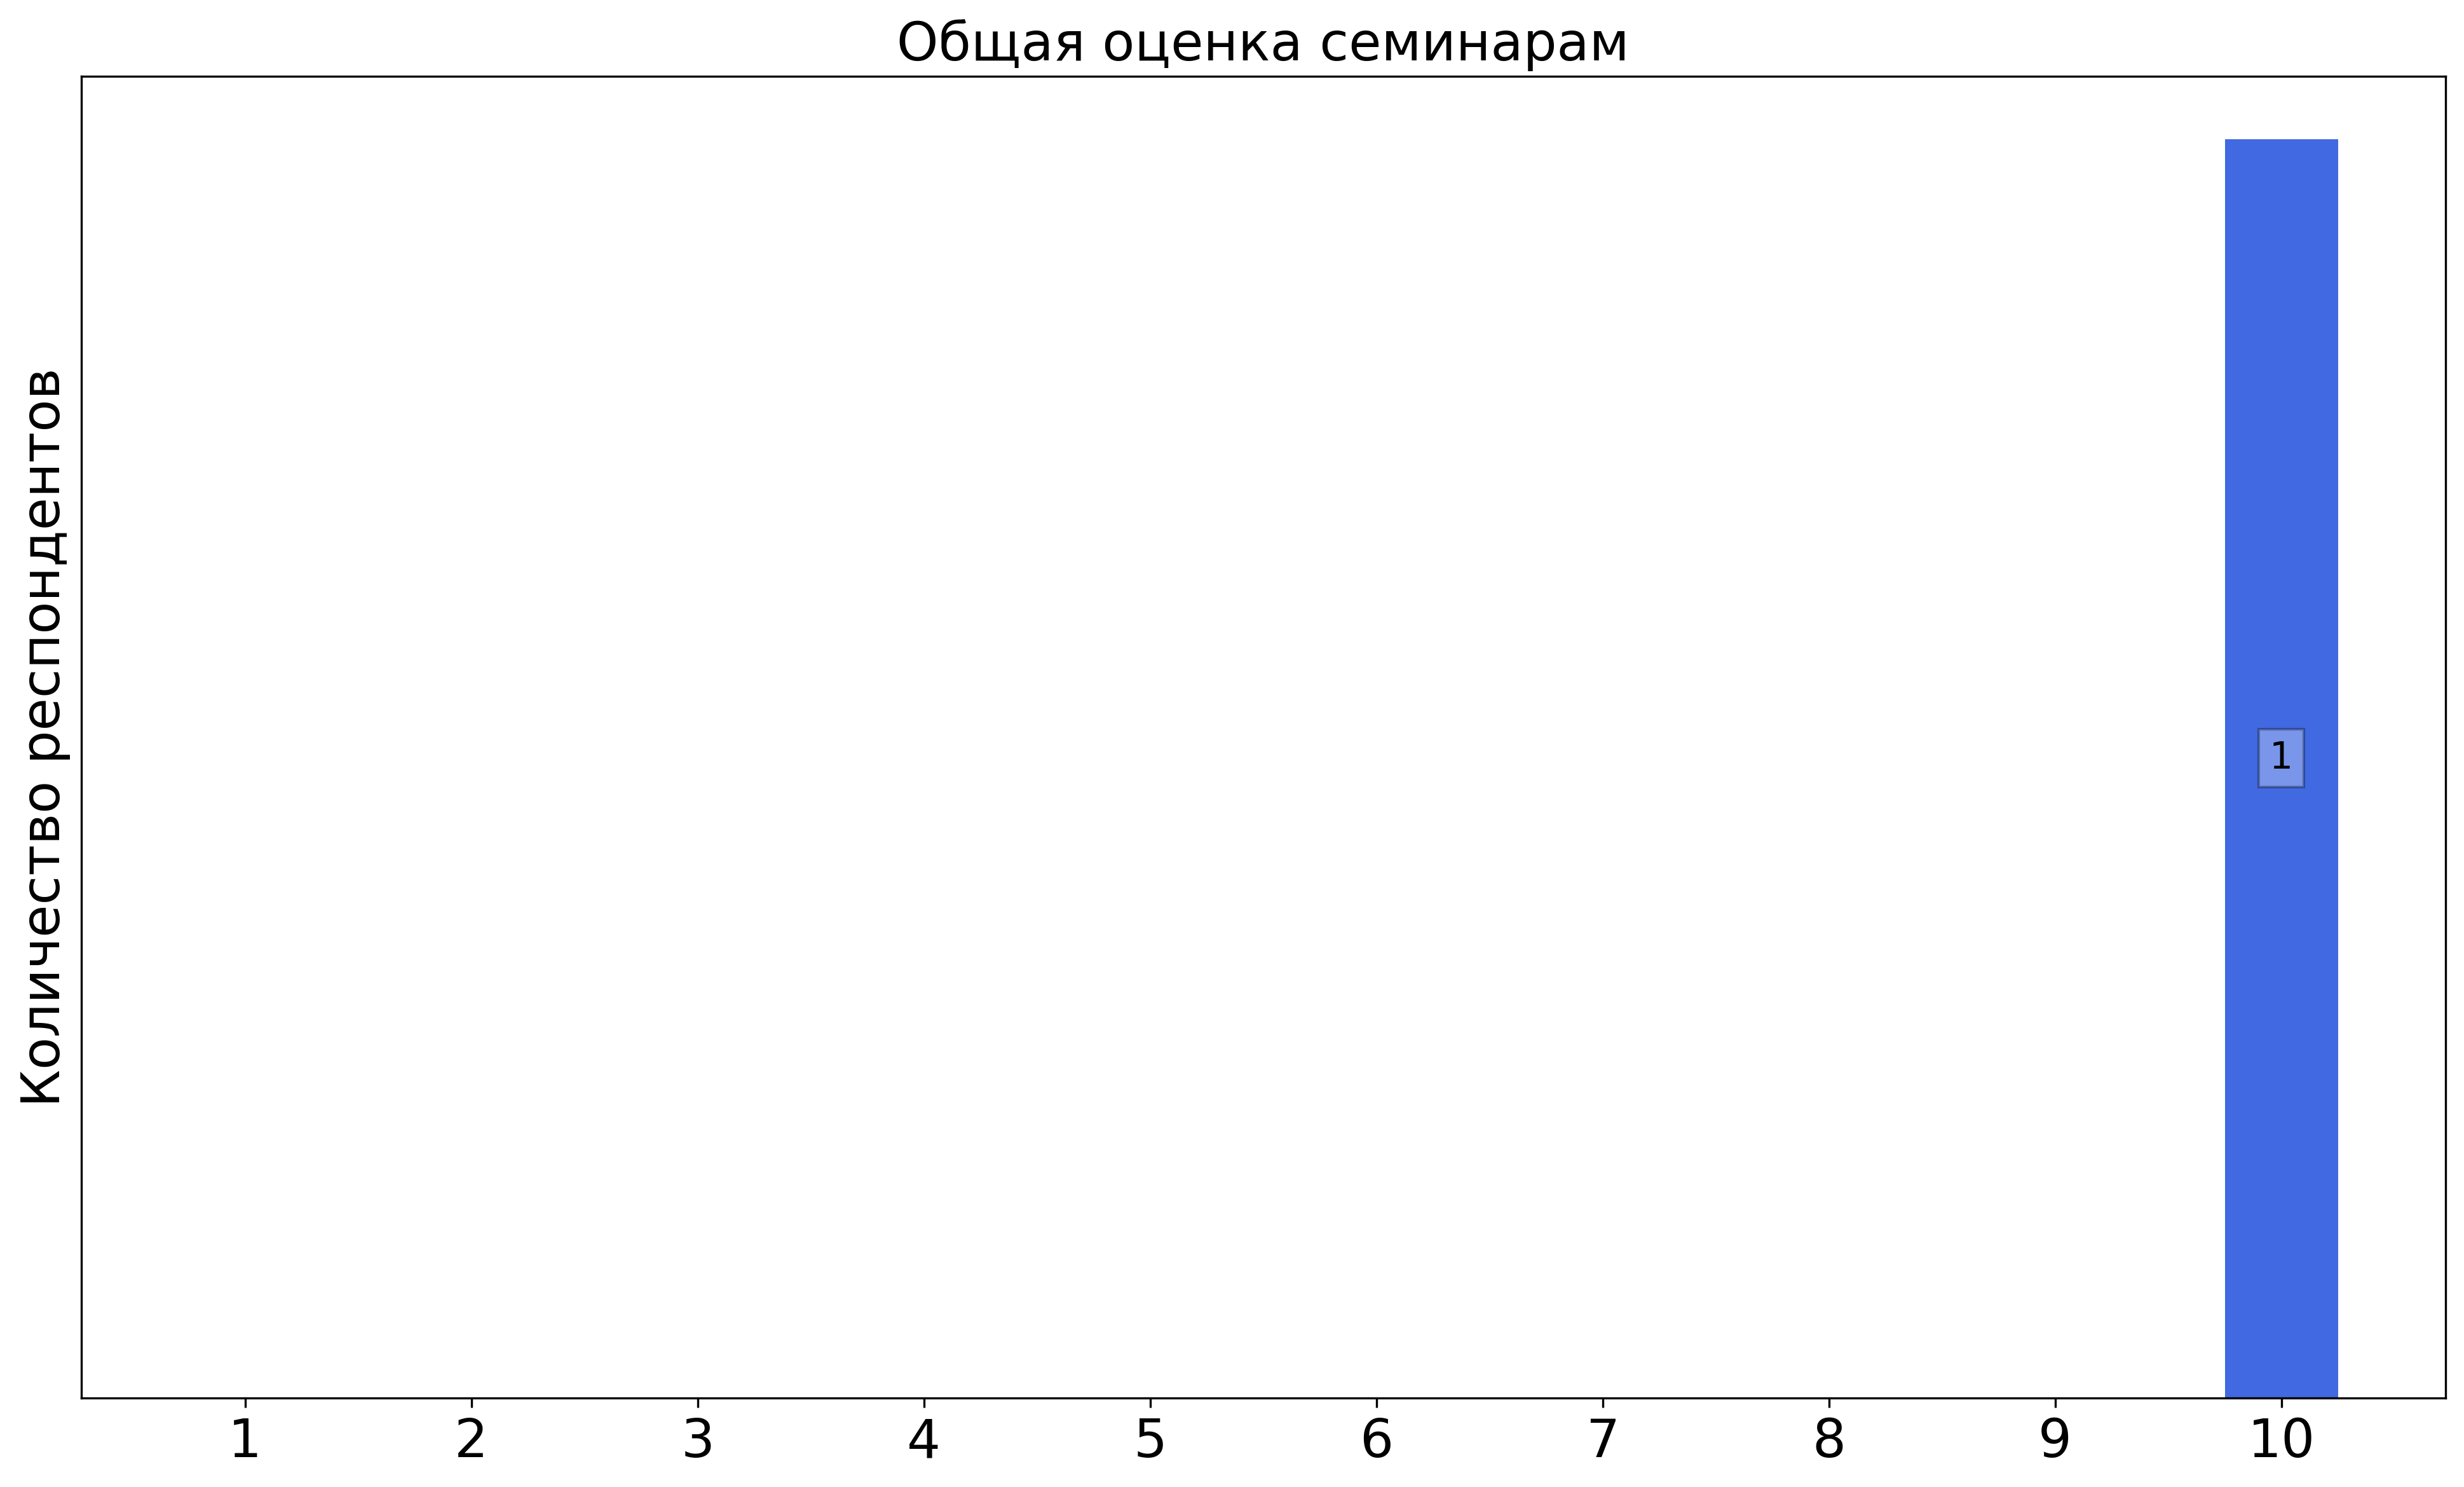
\includegraphics[width=\textwidth]{images/2 course/Общая физика - электричество и магнетизм/seminarists-marks-Максимычев А.В.-3.png}
			\end{subfigure}	
			\caption{Оценки респондентов о качестве преподавания семинаров}
		\end{figure}


	\subsubsection{Отзыв студентов о семинарах. Семинарист: Мирончук Е.С.}
		\begin{figure}[H]
			\centering
			\begin{subfigure}[b]{0.45\textwidth}
				\centering
				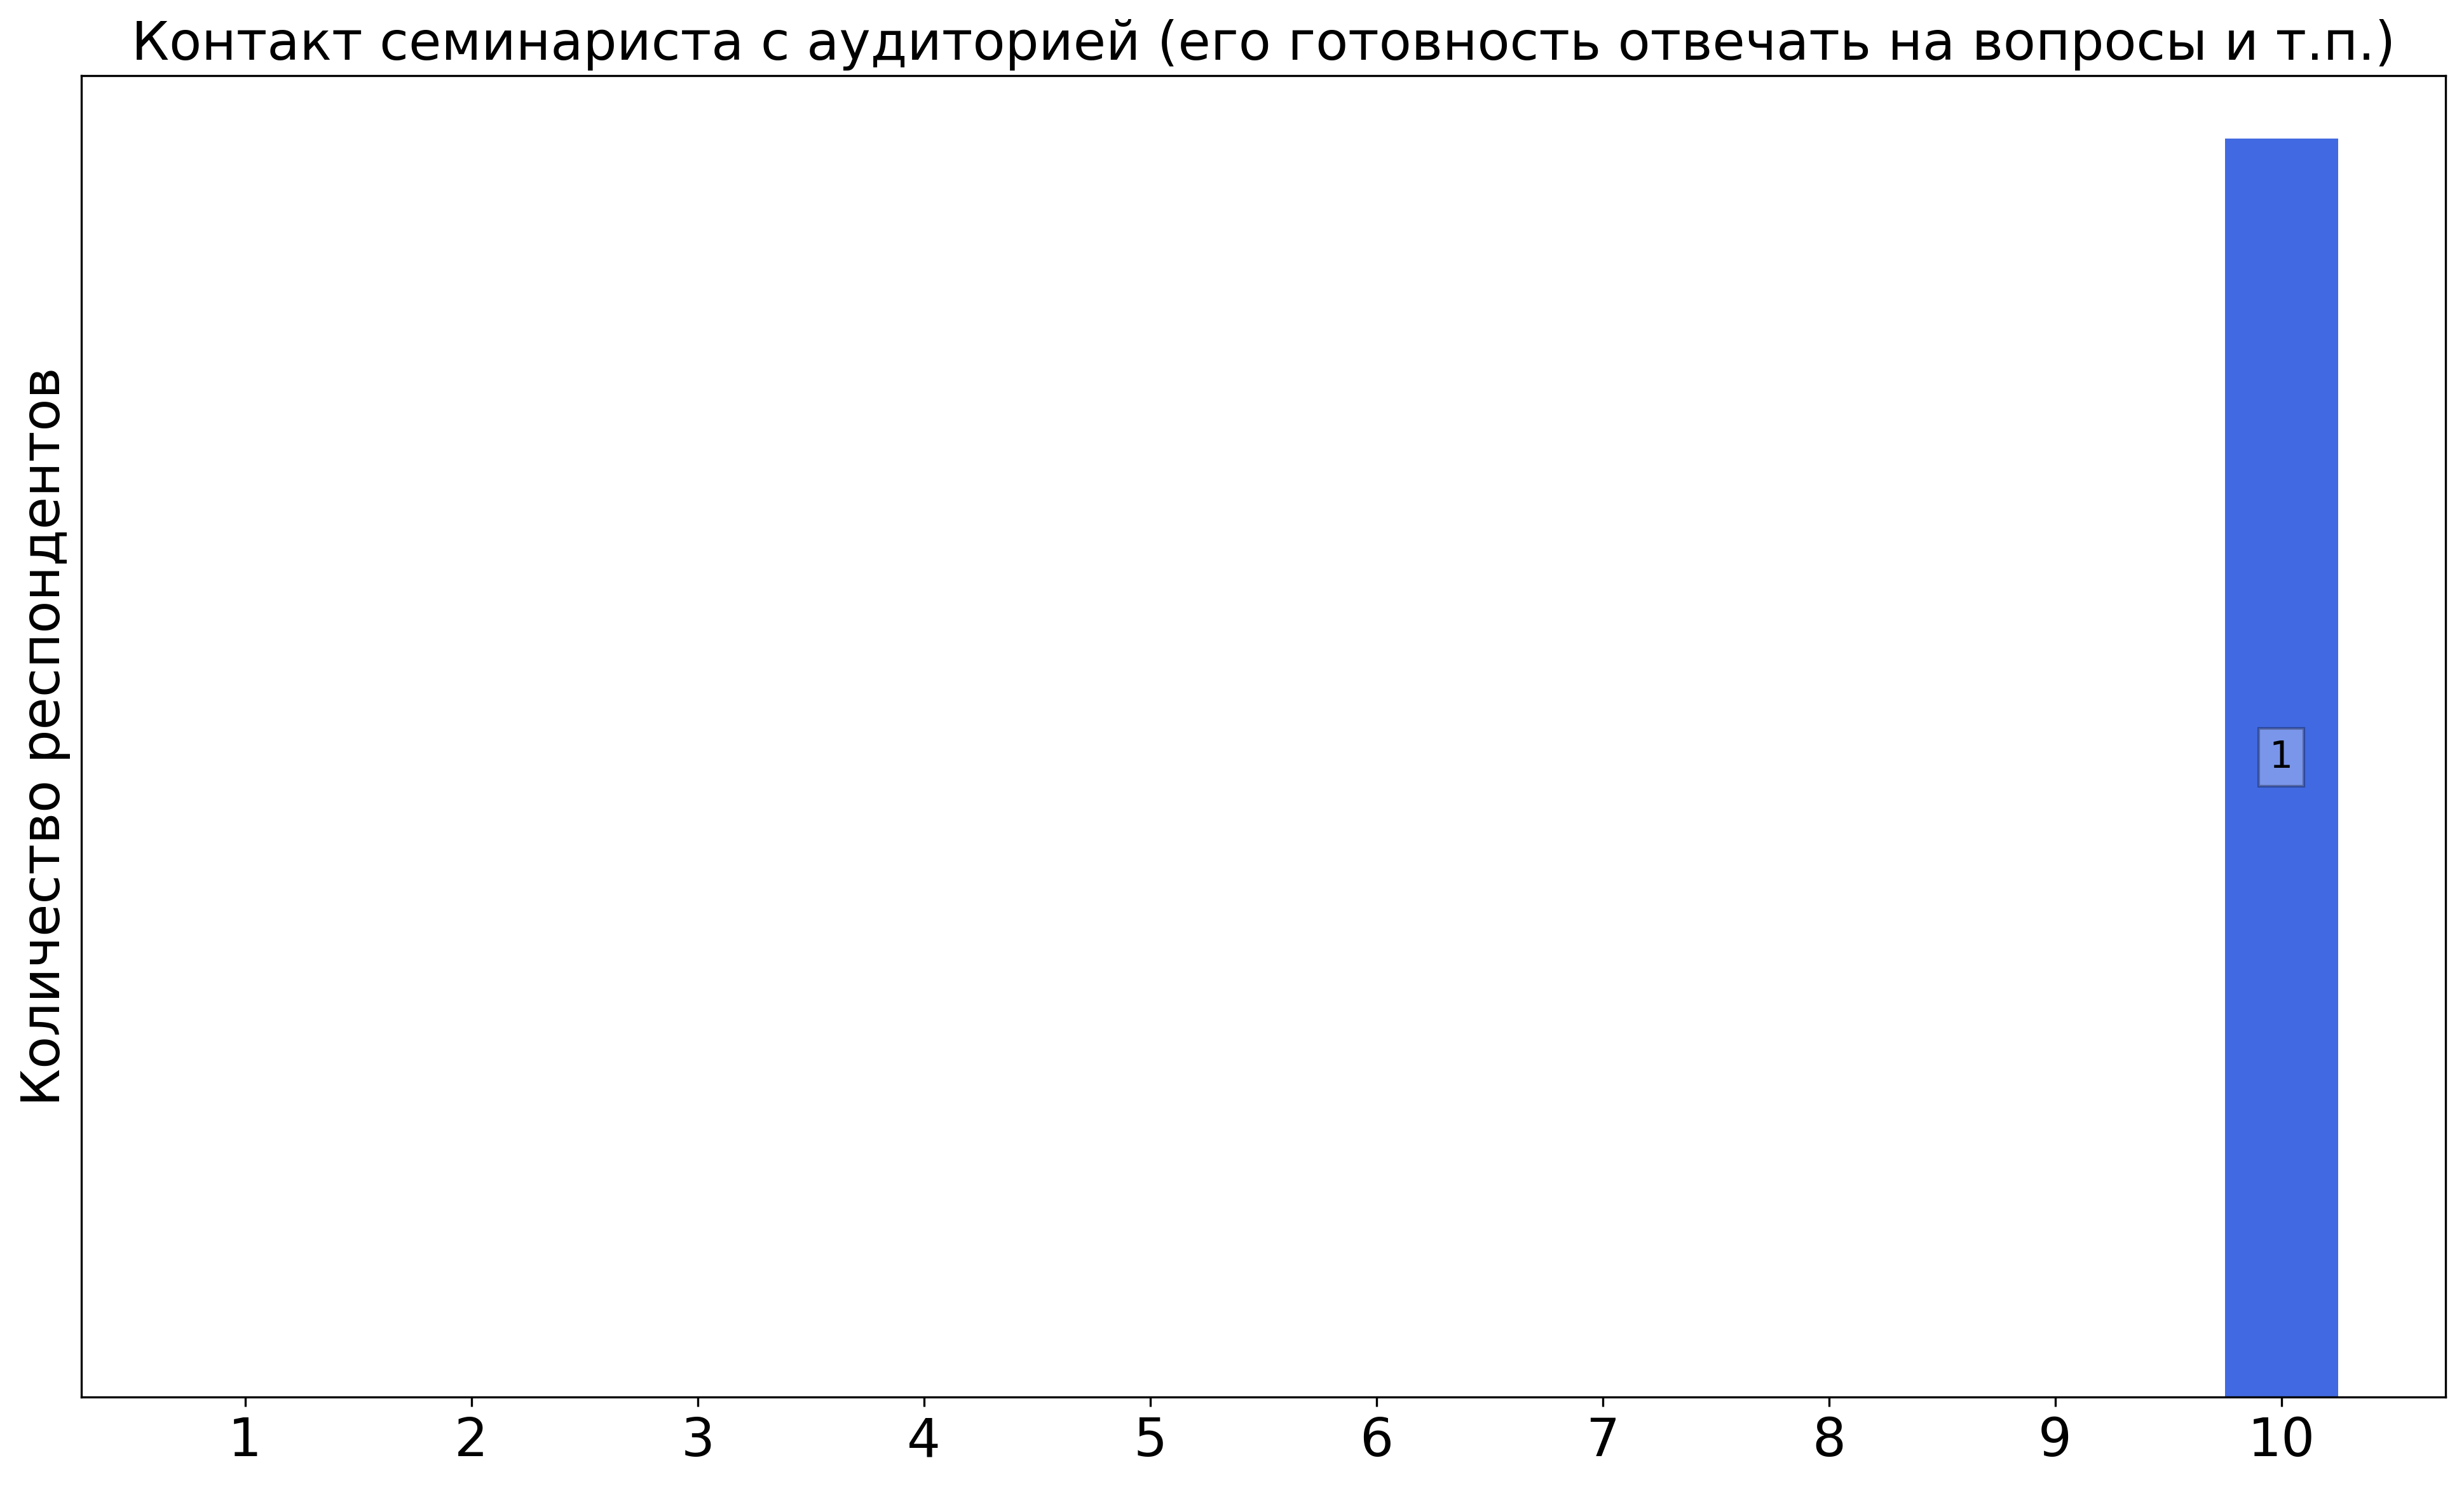
\includegraphics[width=\textwidth]{images/2 course/Общая физика - электричество и магнетизм/seminarists-marks-Мирончук Е.С.-0.png}
			\end{subfigure}
			\begin{subfigure}[b]{0.45\textwidth}
				\centering
				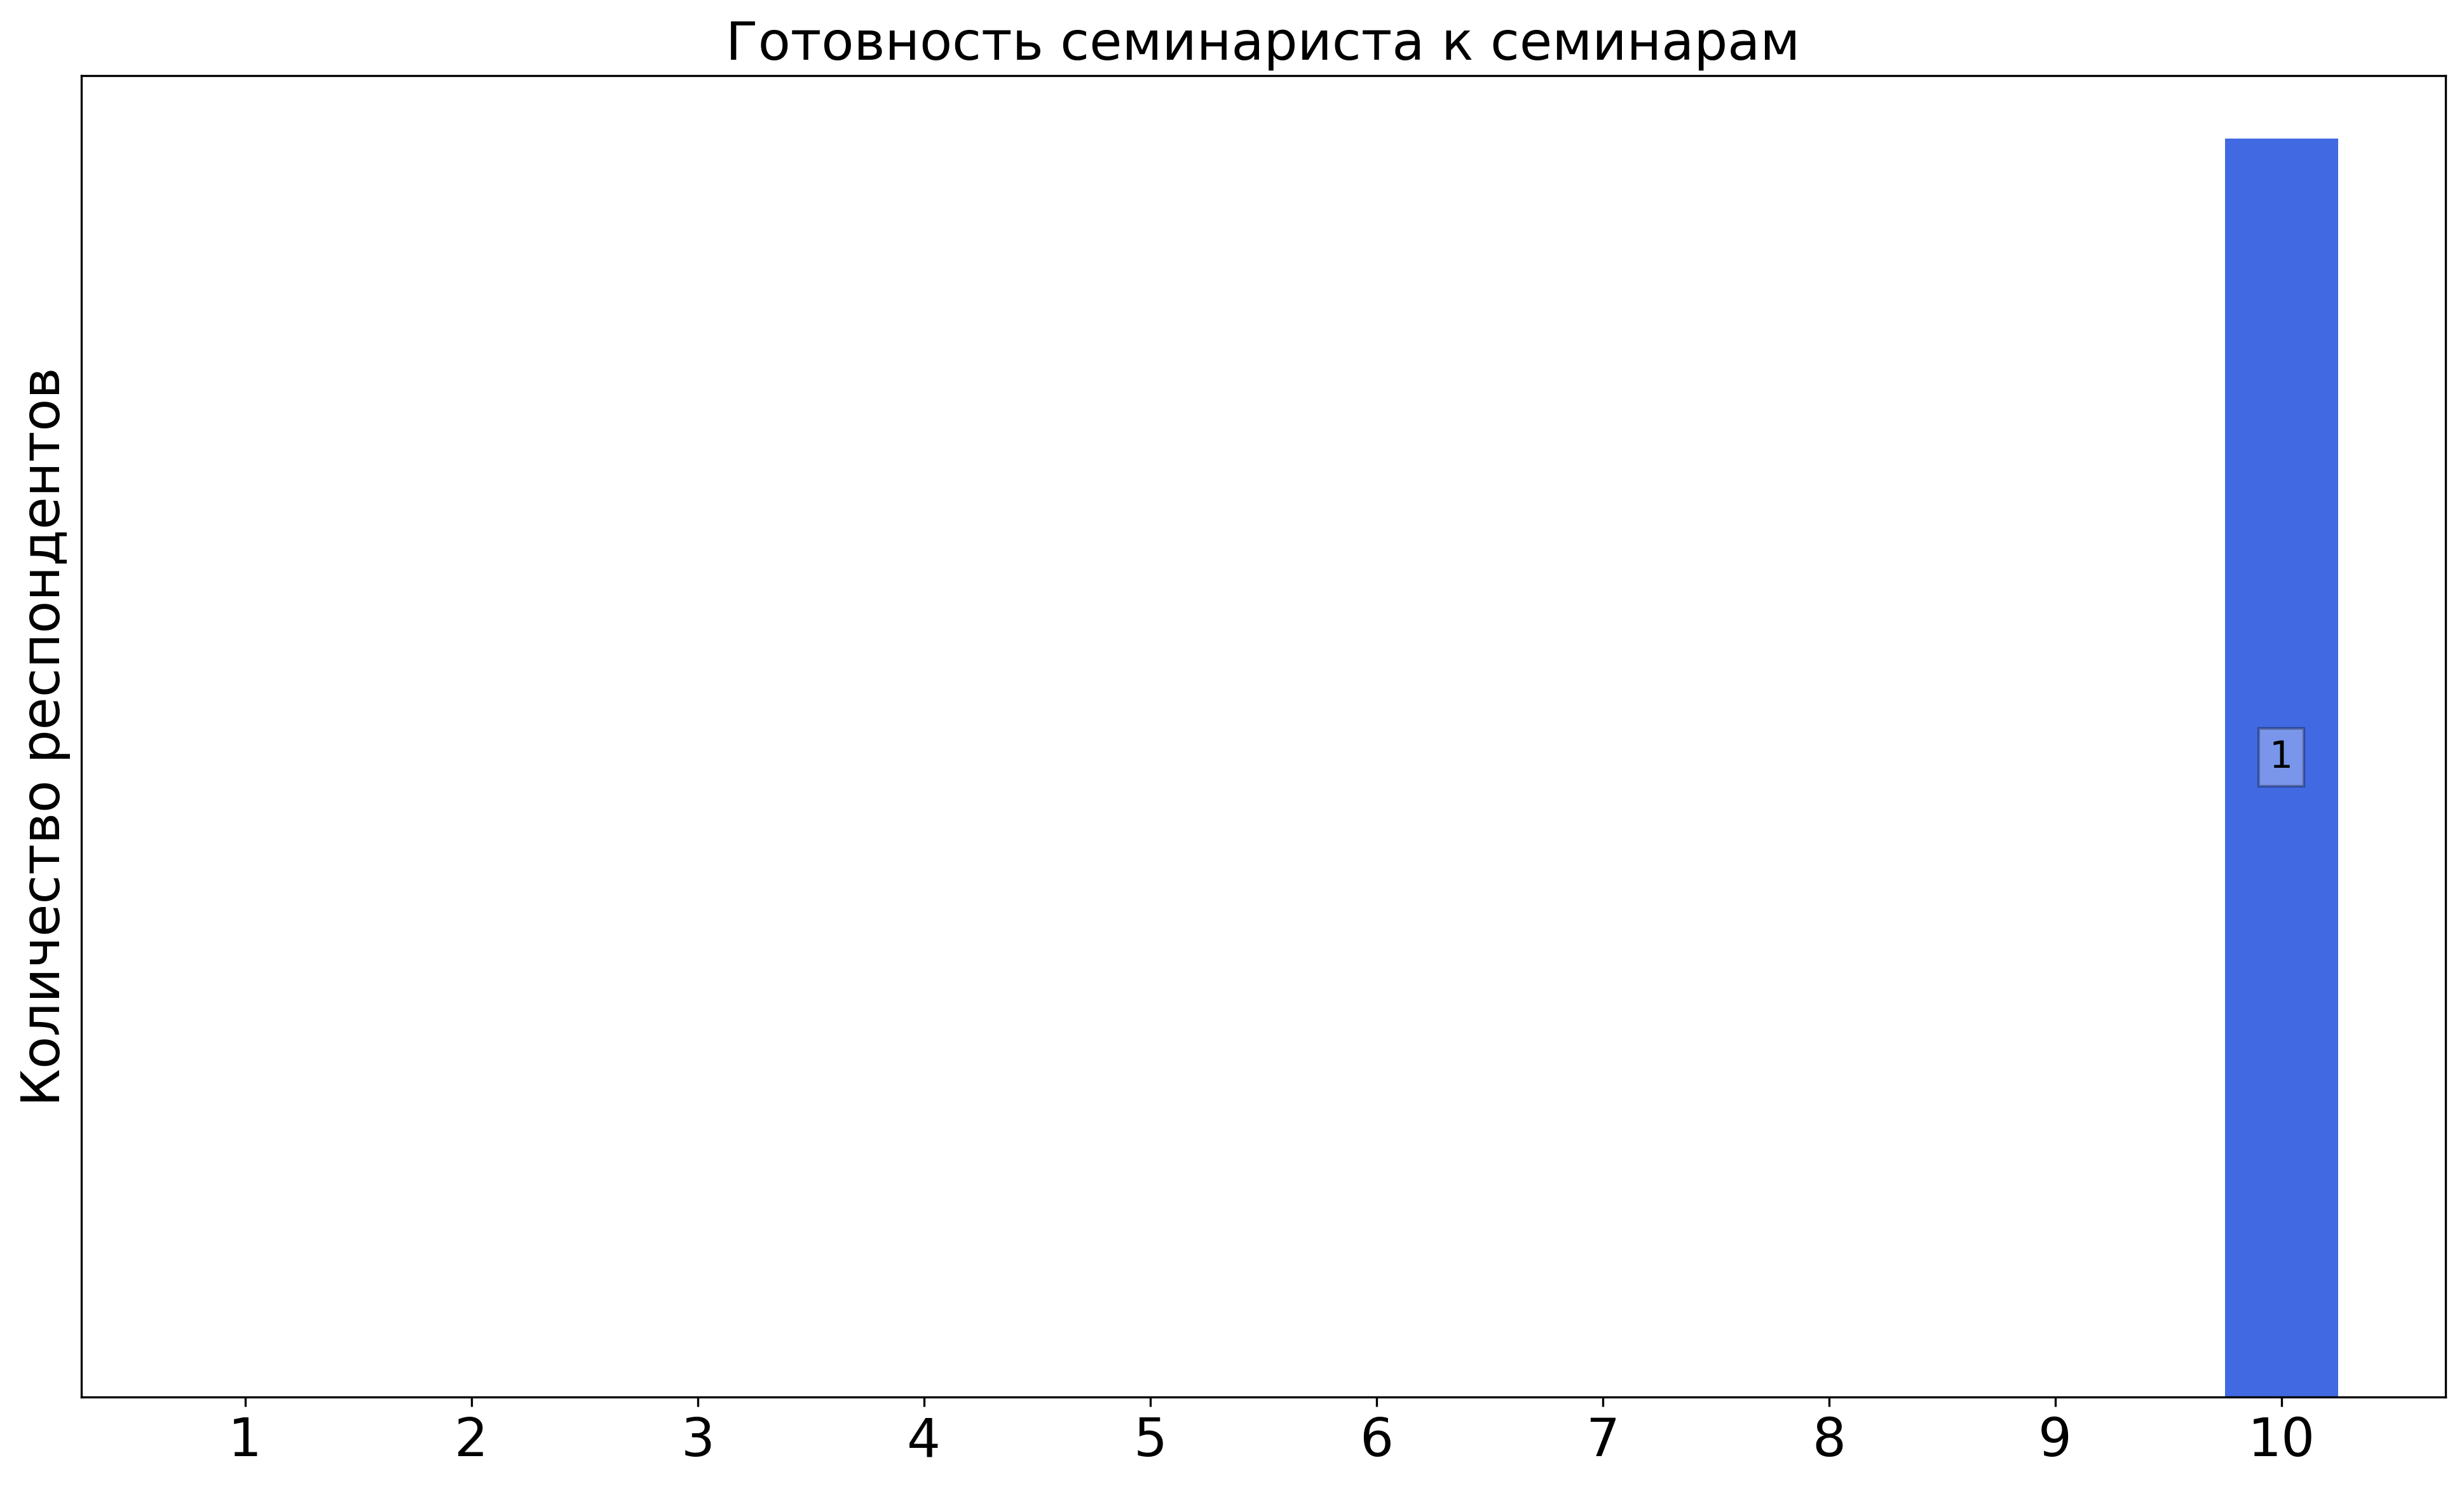
\includegraphics[width=\textwidth]{images/2 course/Общая физика - электричество и магнетизм/seminarists-marks-Мирончук Е.С.-1.png}
			\end{subfigure}
			\begin{subfigure}[b]{0.45\textwidth}
				\centering
				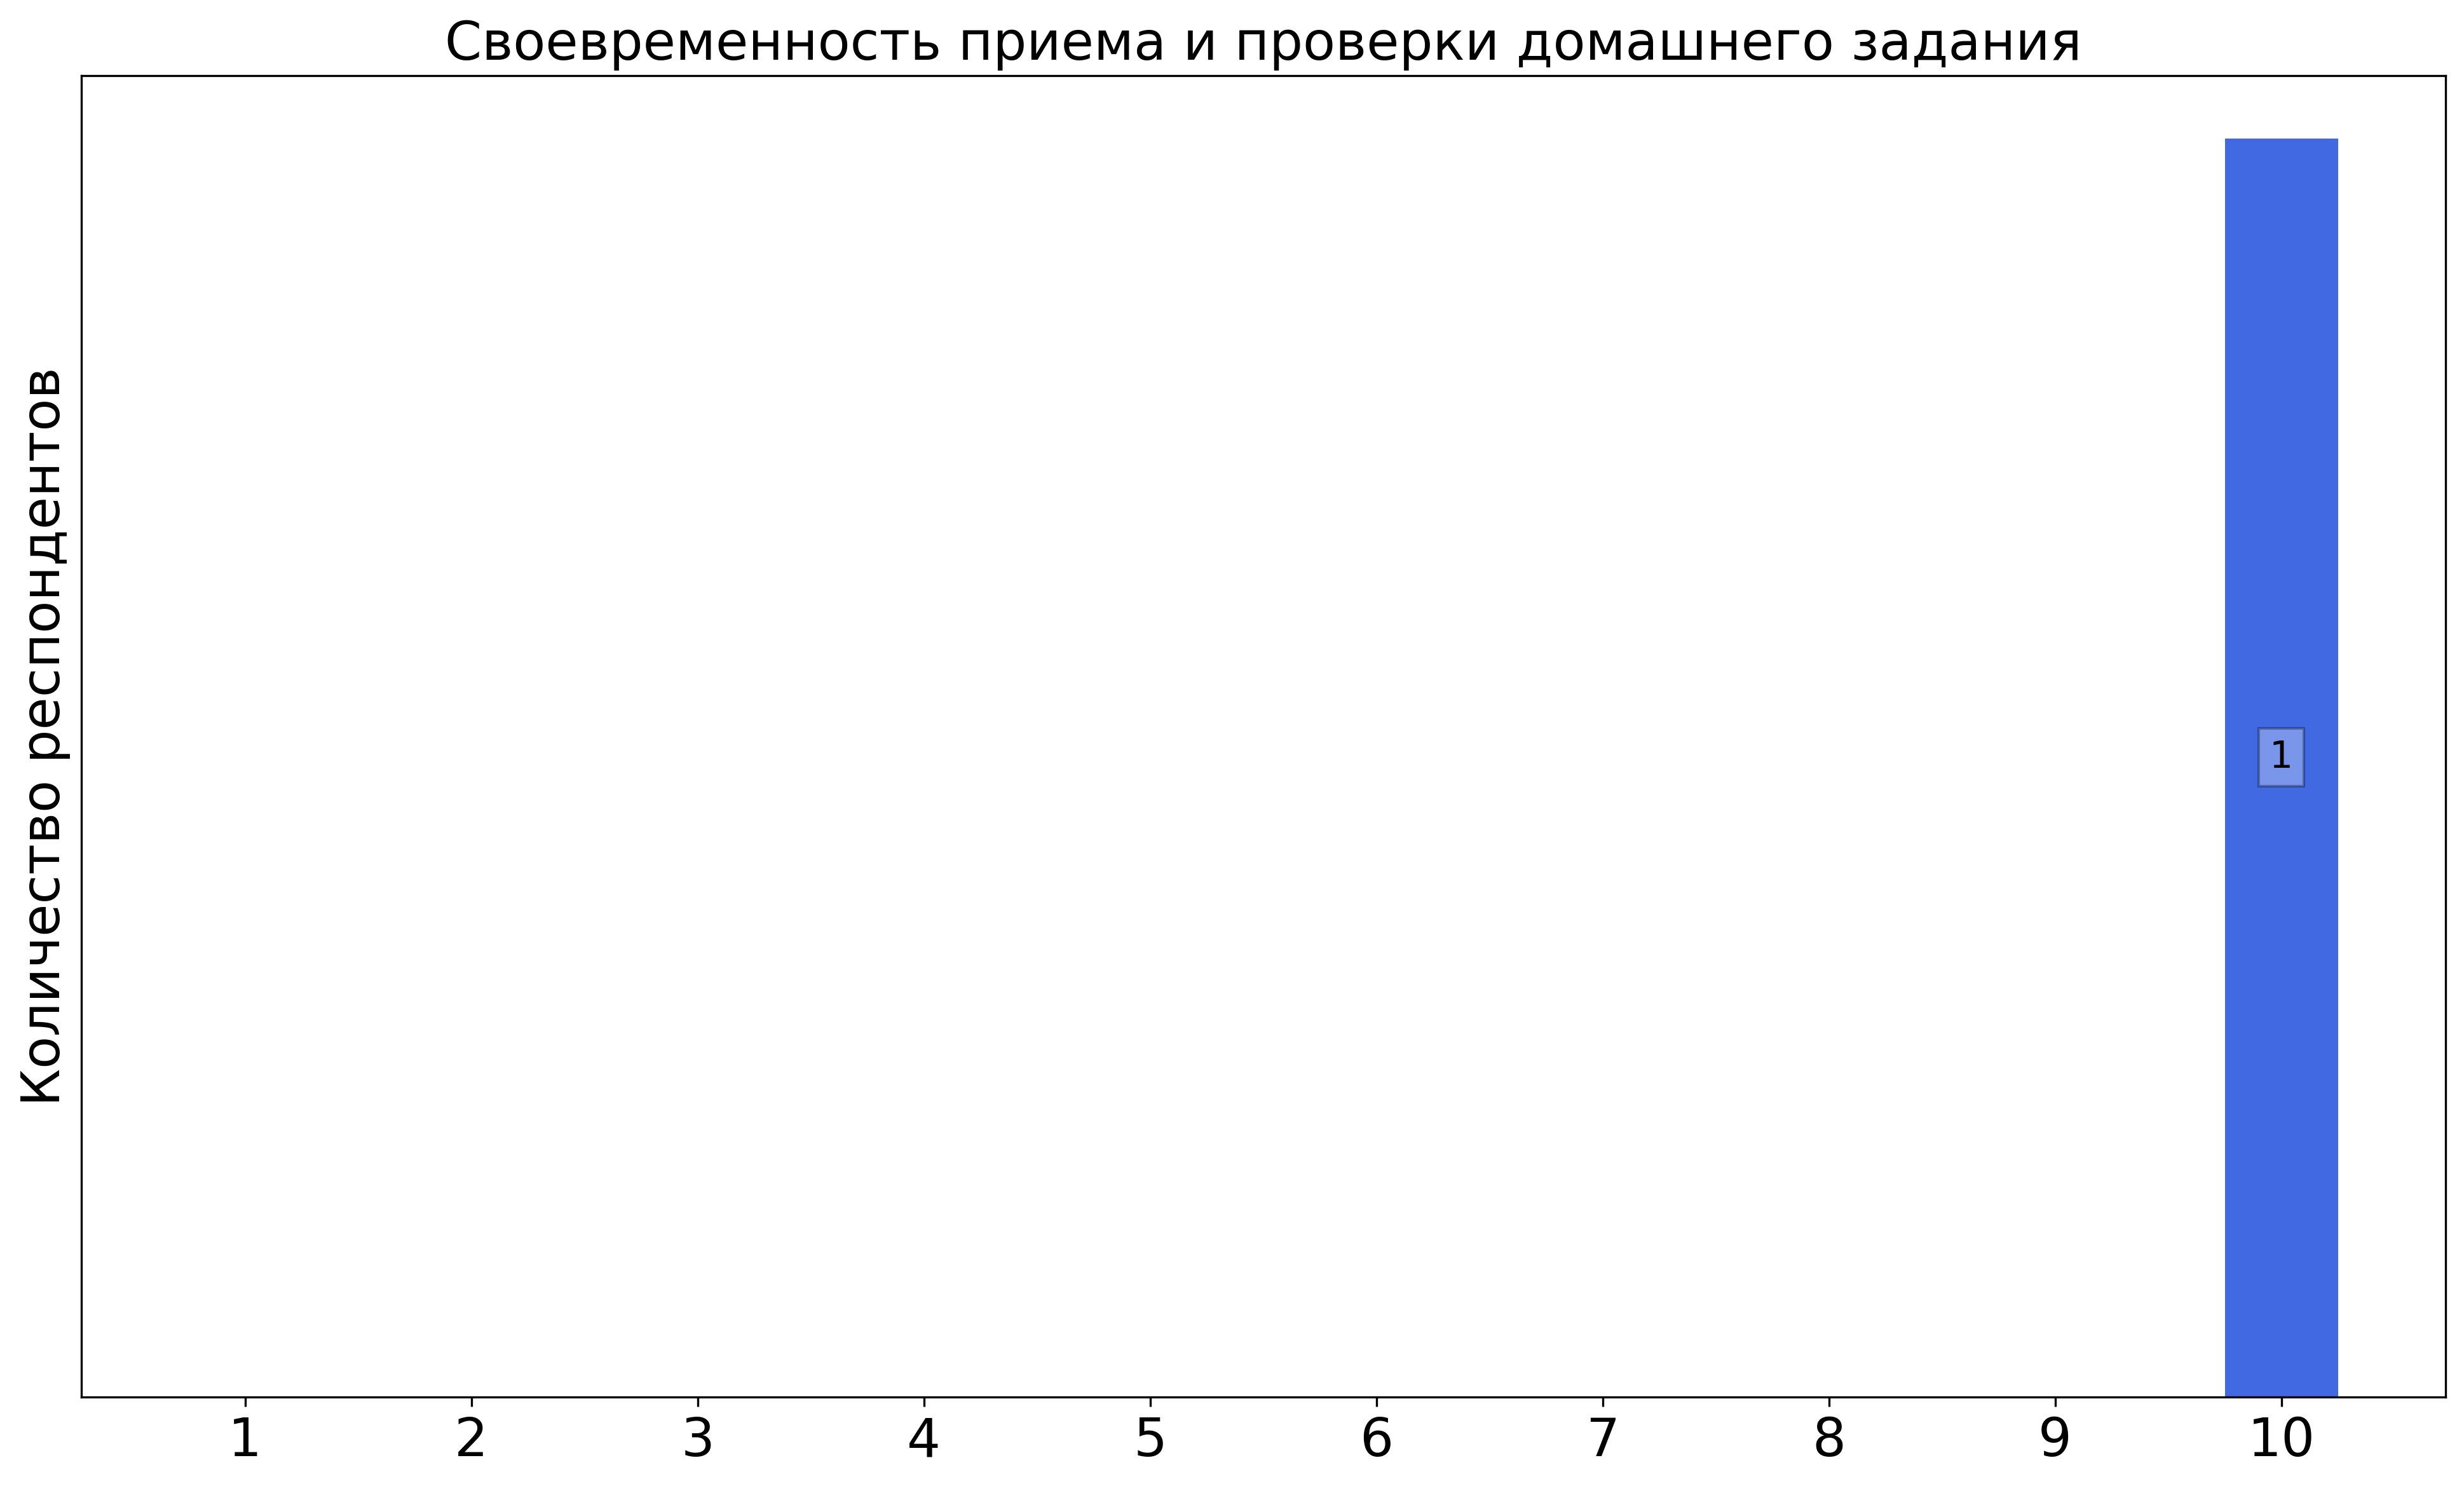
\includegraphics[width=\textwidth]{images/2 course/Общая физика - электричество и магнетизм/seminarists-marks-Мирончук Е.С.-2.png}
			\end{subfigure}
			\begin{subfigure}[b]{0.45\textwidth}
				\centering
				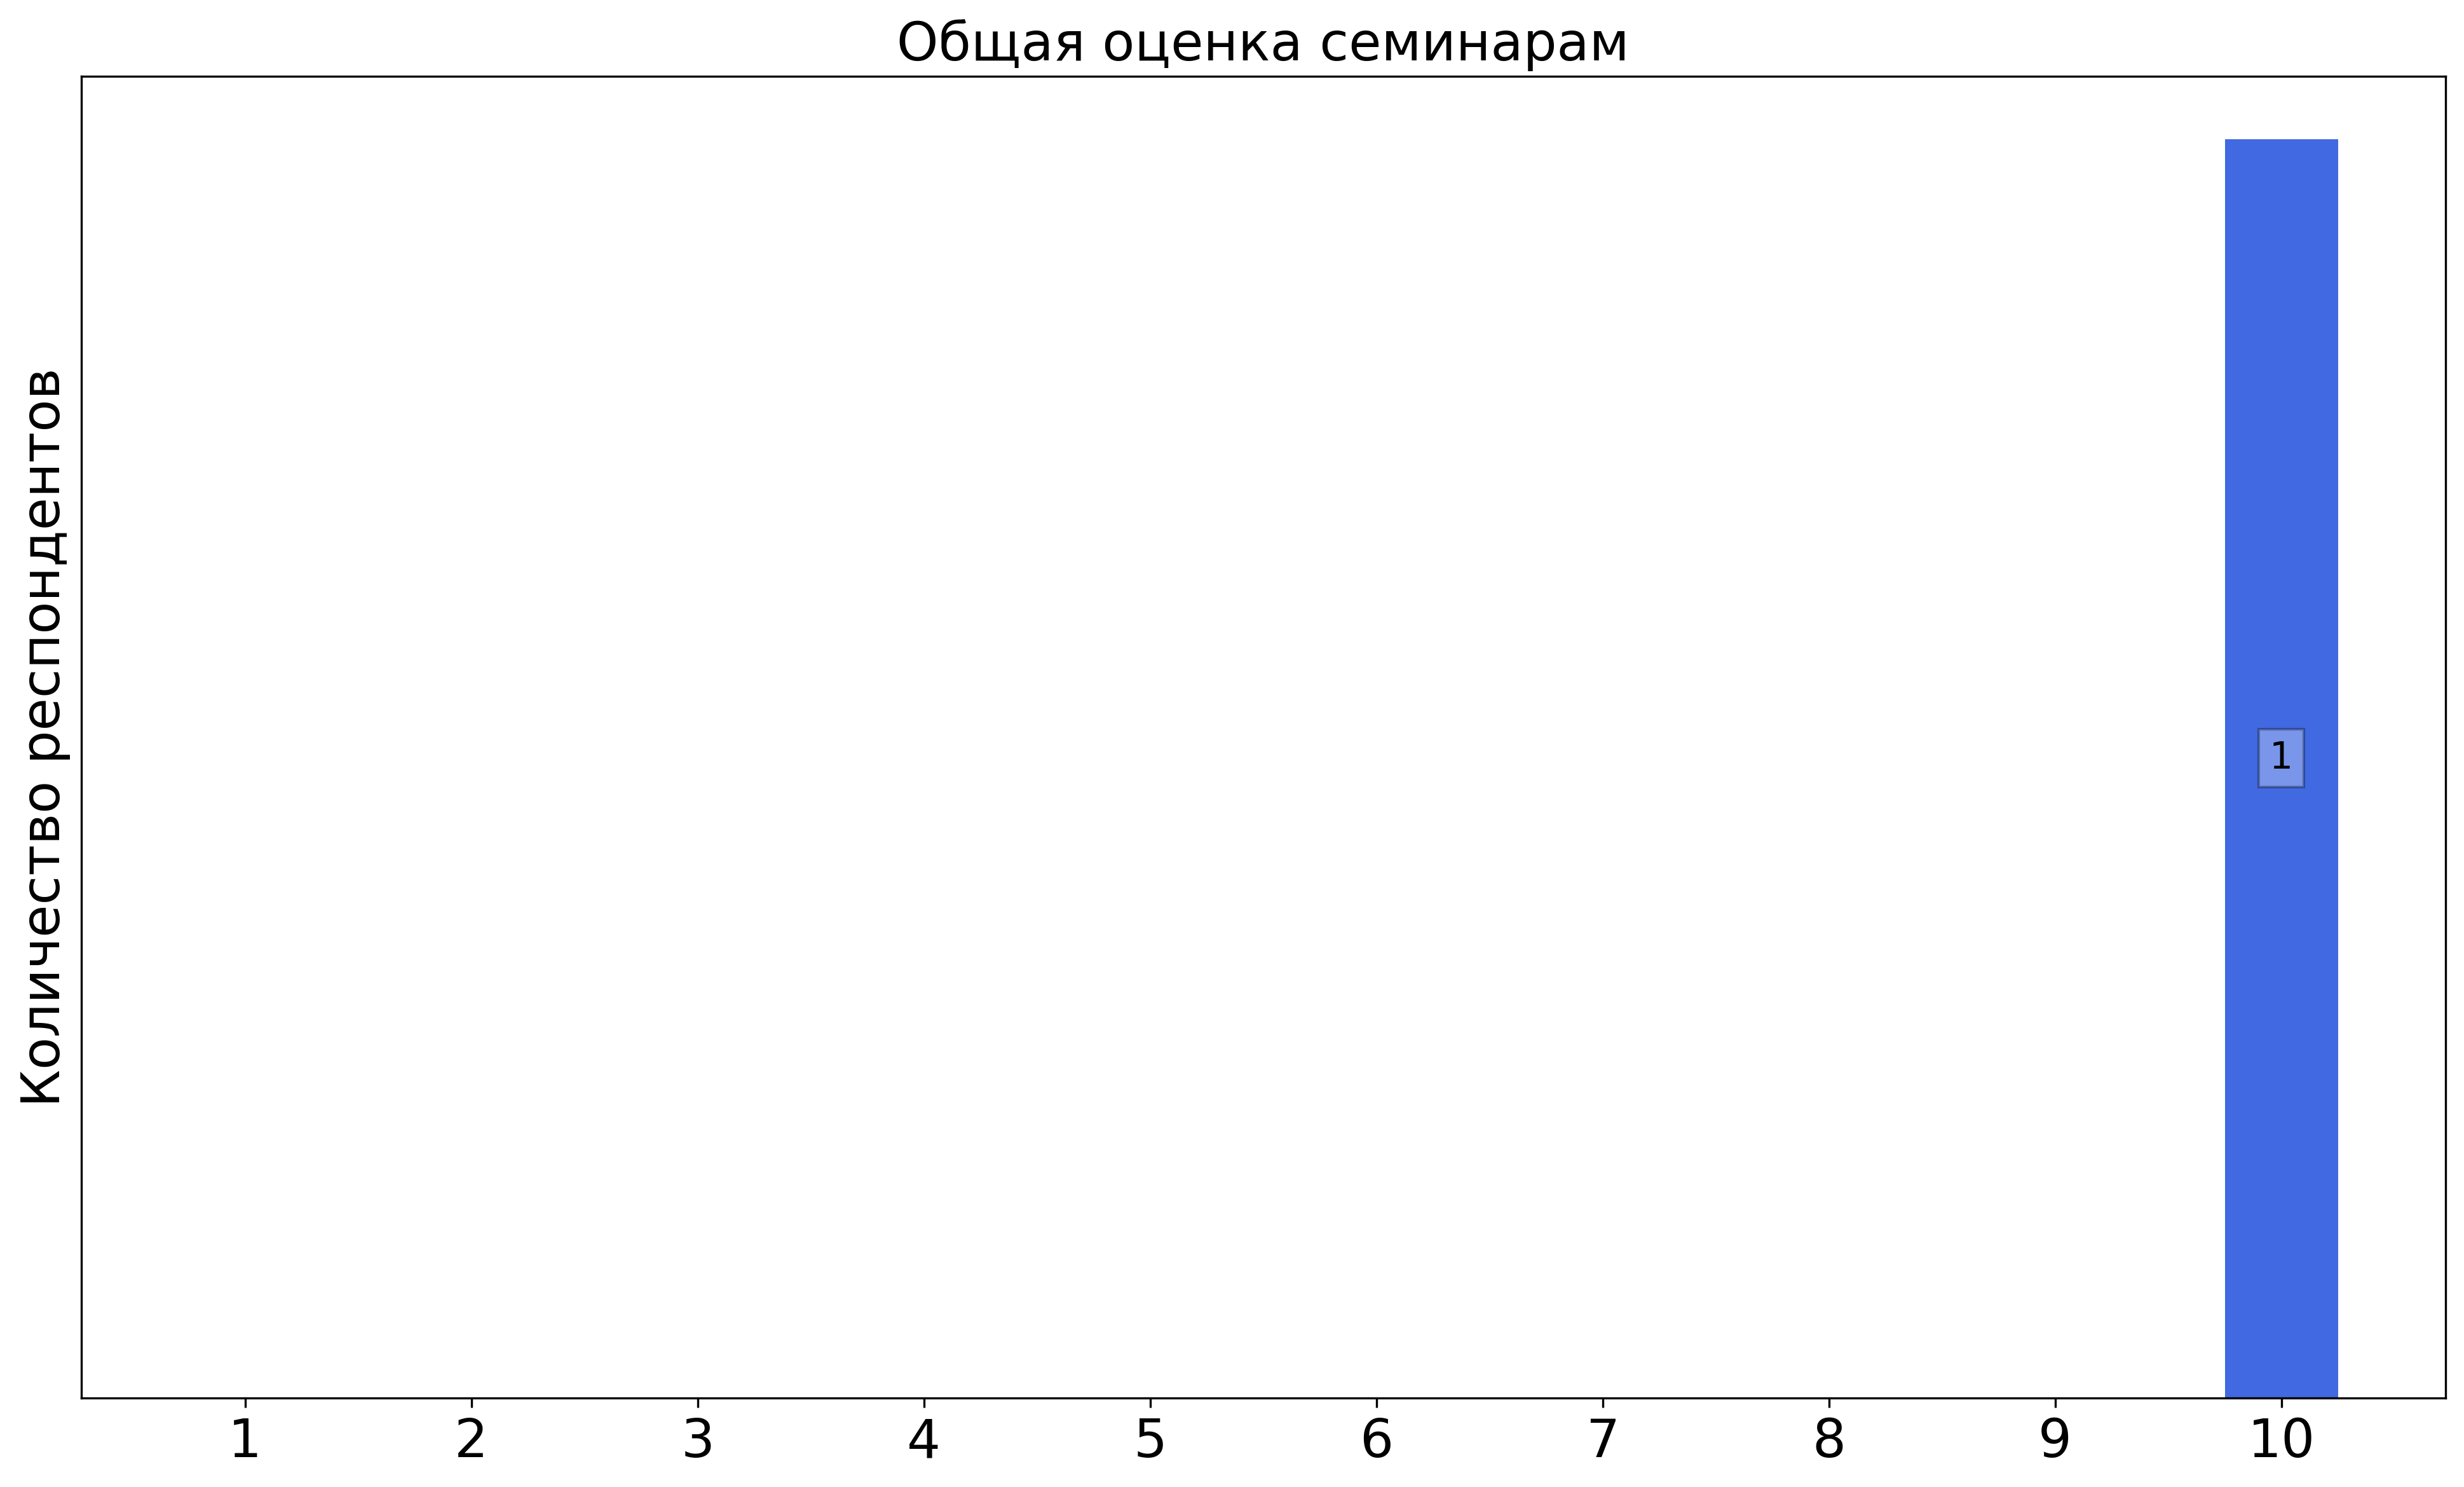
\includegraphics[width=\textwidth]{images/2 course/Общая физика - электричество и магнетизм/seminarists-marks-Мирончук Е.С.-3.png}
			\end{subfigure}	
			\caption{Оценки респондентов о качестве преподавания семинаров}
		\end{figure}

	
	\subsubsection{Отзыв студентов о семинарах. Семинарист: Овчинкин В.А.}
		\begin{figure}[H]
			\centering
			\begin{subfigure}[b]{0.45\textwidth}
				\centering
				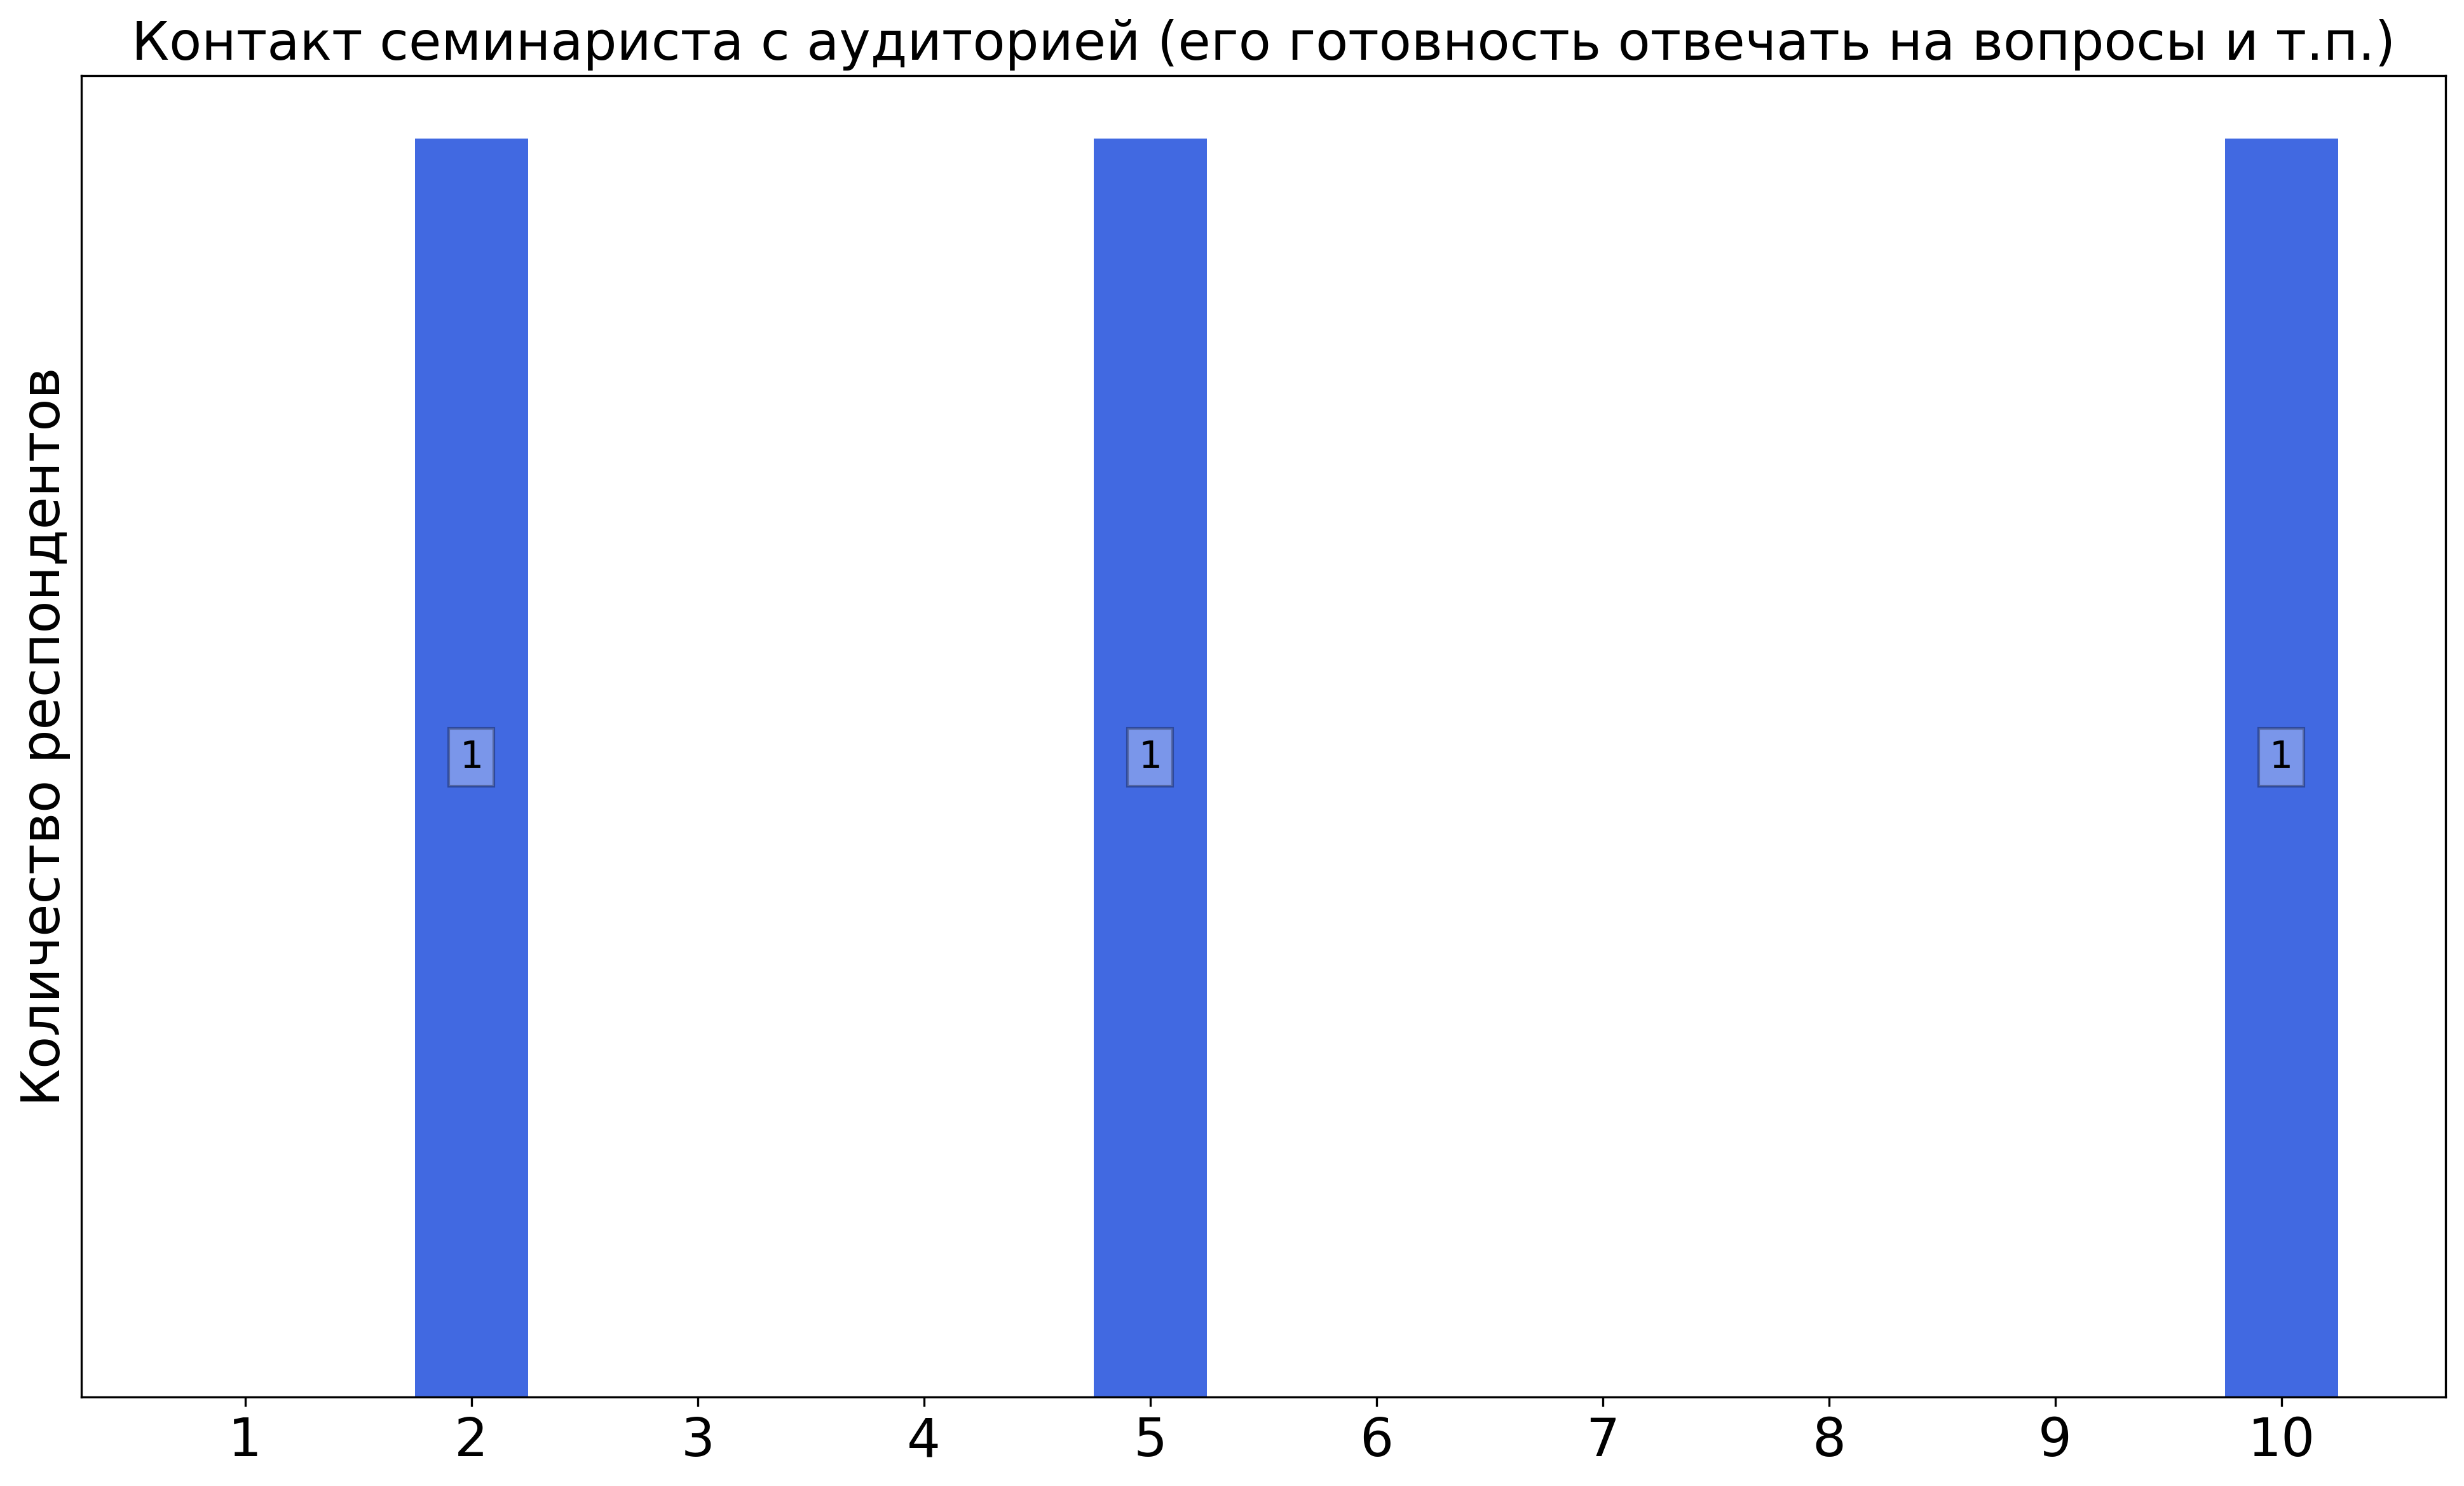
\includegraphics[width=\textwidth]{images/2 course/Общая физика - электричество и магнетизм/seminarists-marks-Овчинкин В.А.-0.png}
			\end{subfigure}
			\begin{subfigure}[b]{0.45\textwidth}
				\centering
				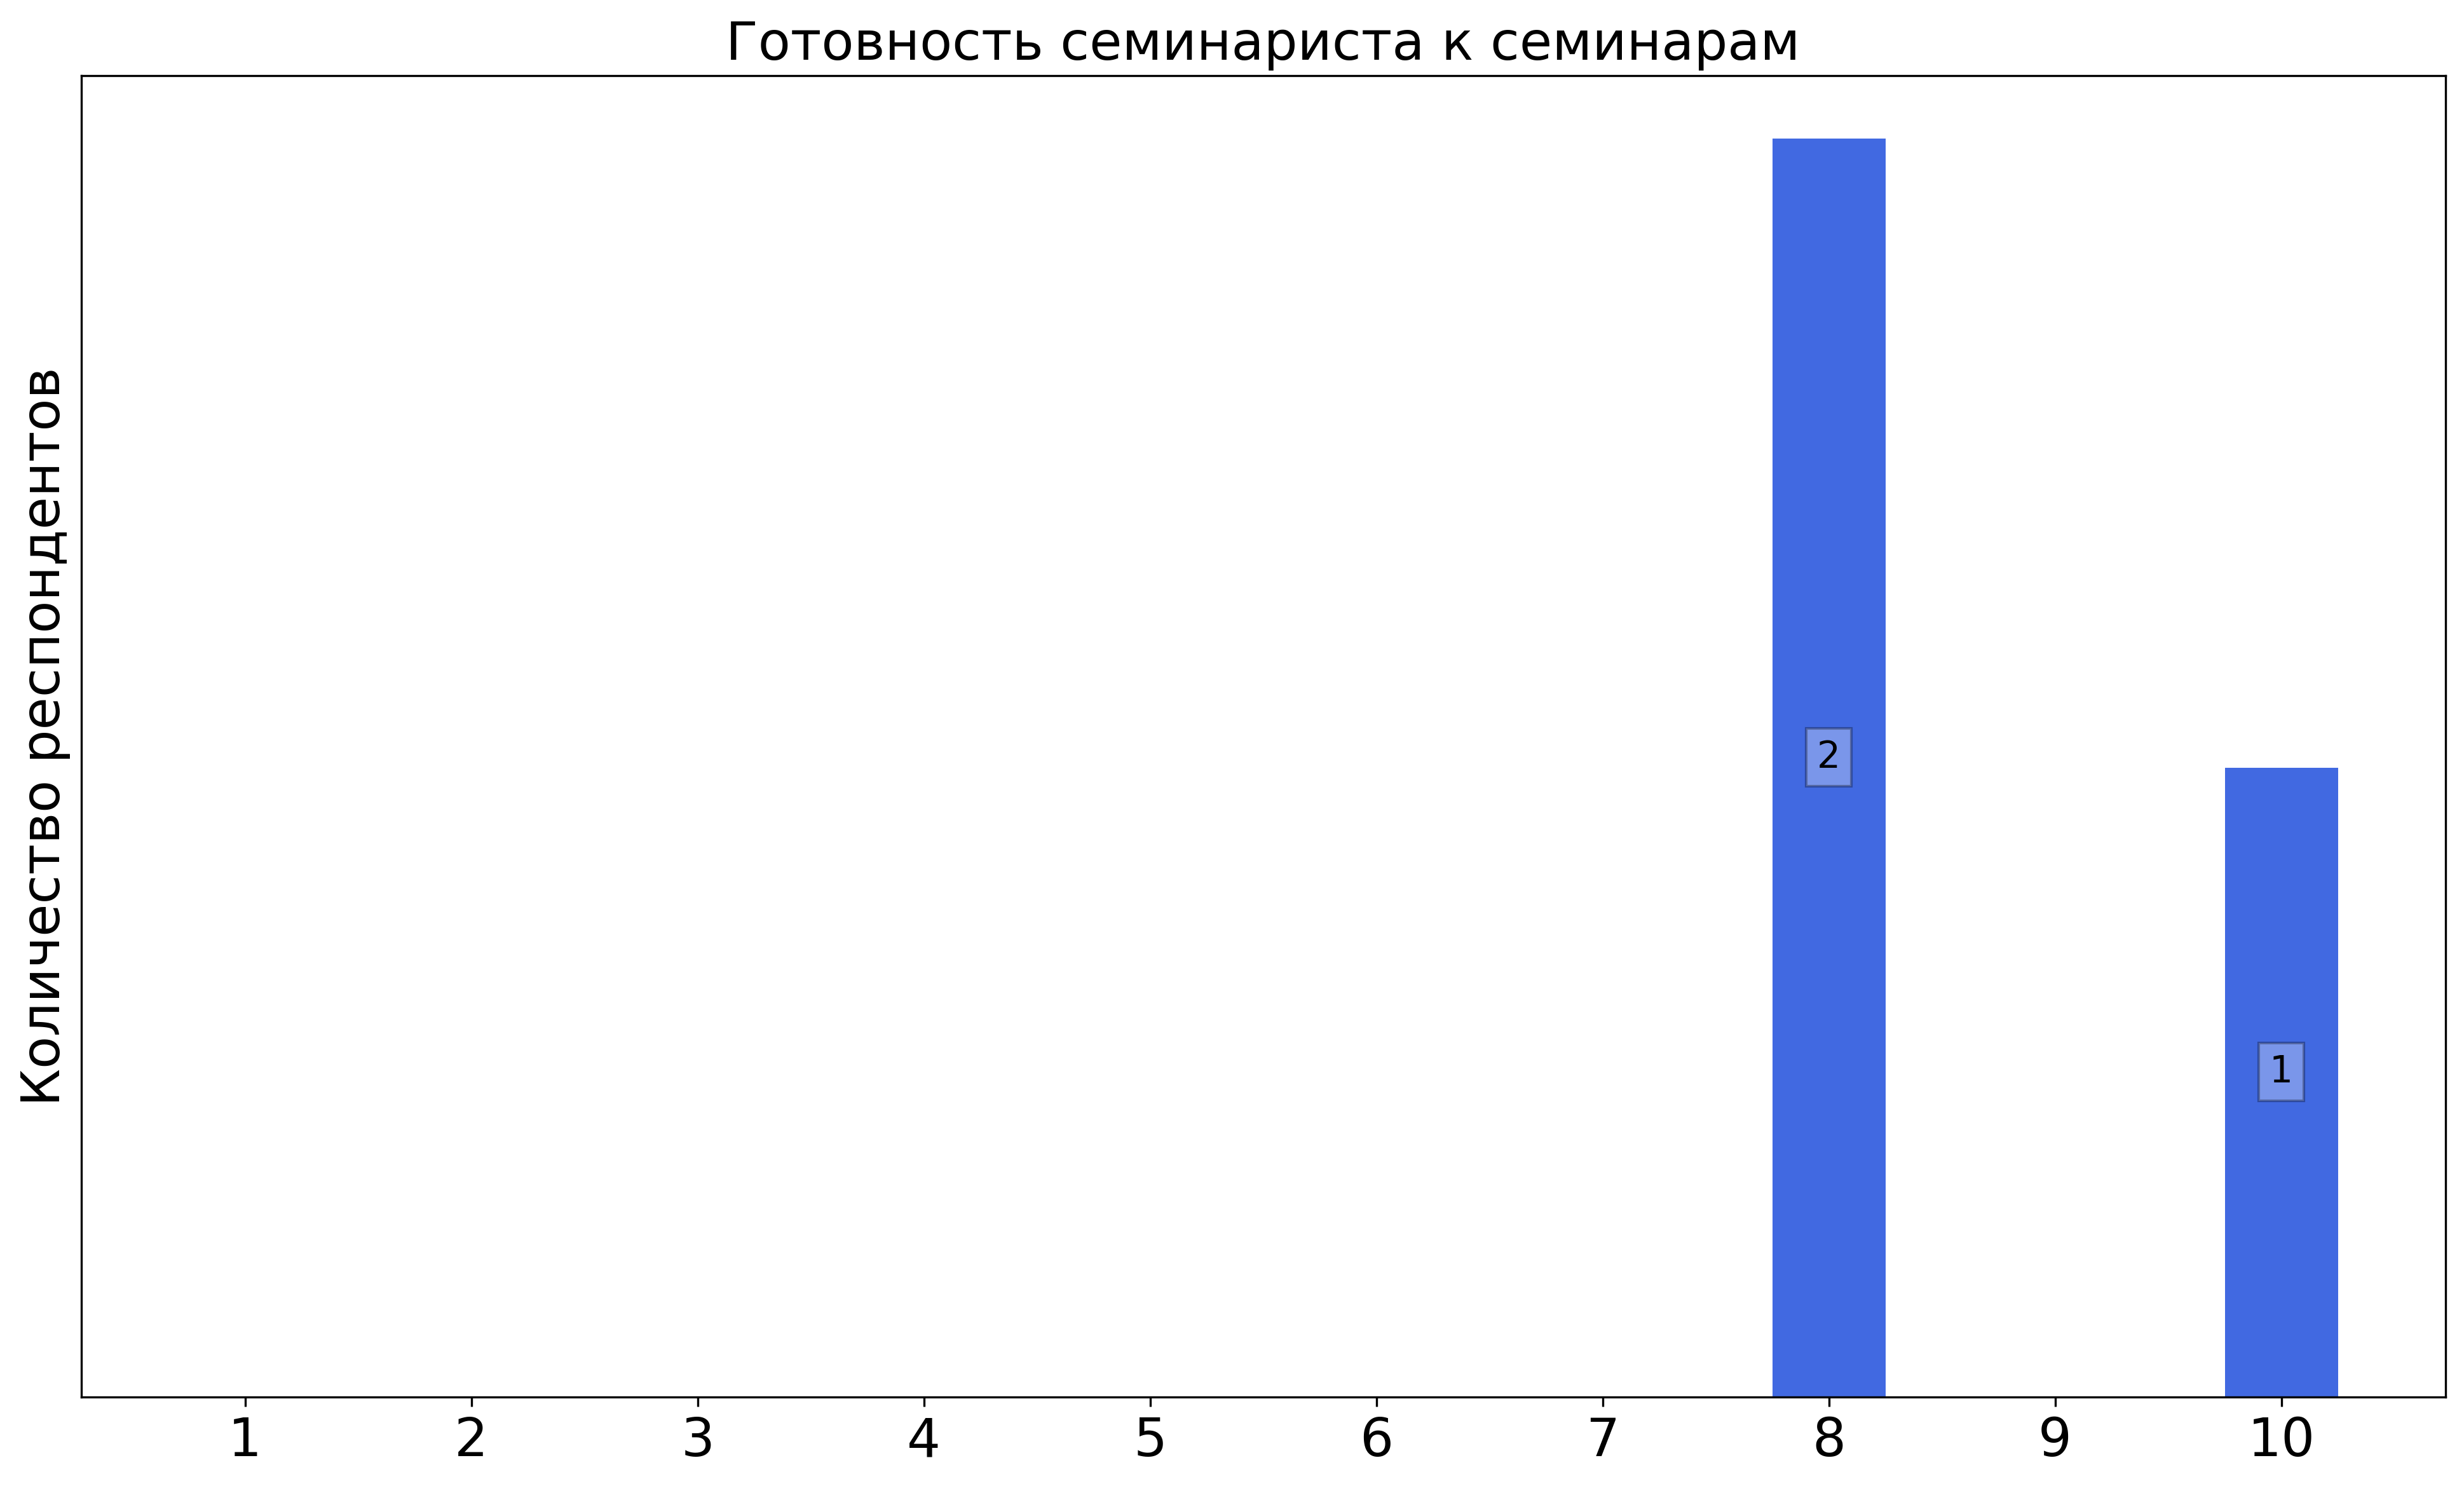
\includegraphics[width=\textwidth]{images/2 course/Общая физика - электричество и магнетизм/seminarists-marks-Овчинкин В.А.-1.png}
			\end{subfigure}
			\begin{subfigure}[b]{0.45\textwidth}
				\centering
				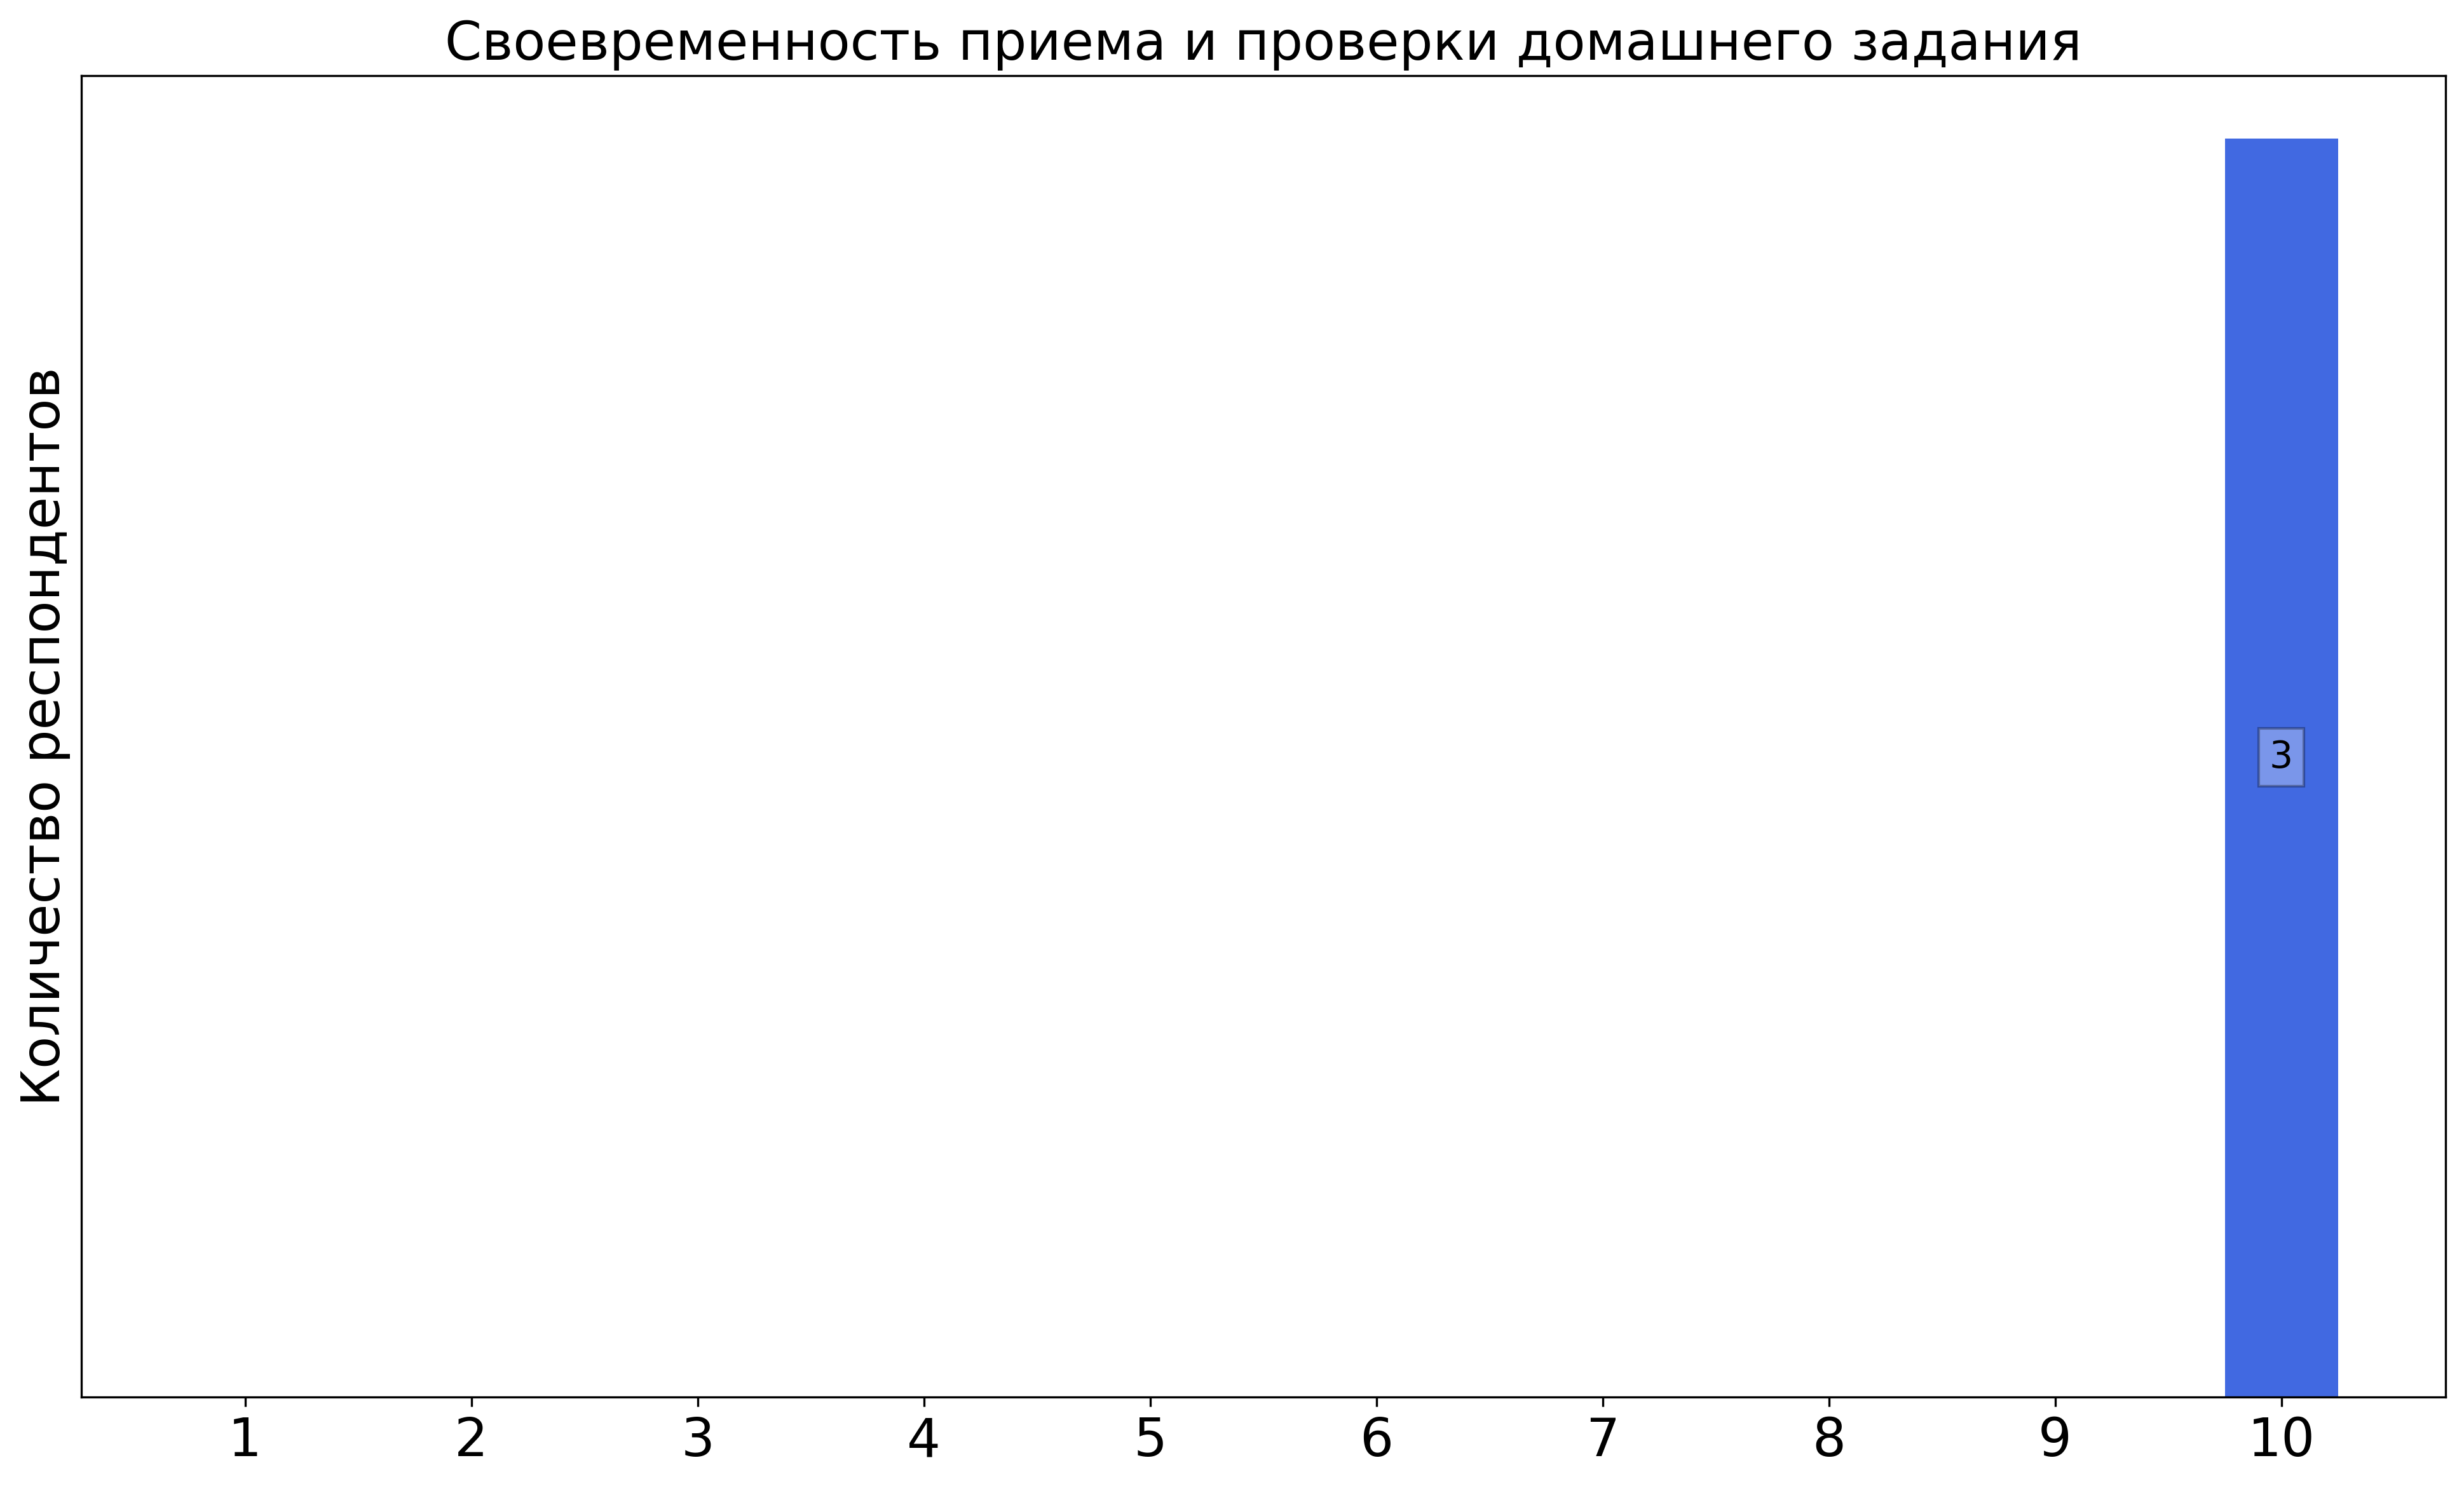
\includegraphics[width=\textwidth]{images/2 course/Общая физика - электричество и магнетизм/seminarists-marks-Овчинкин В.А.-2.png}
			\end{subfigure}
			\begin{subfigure}[b]{0.45\textwidth}
				\centering
				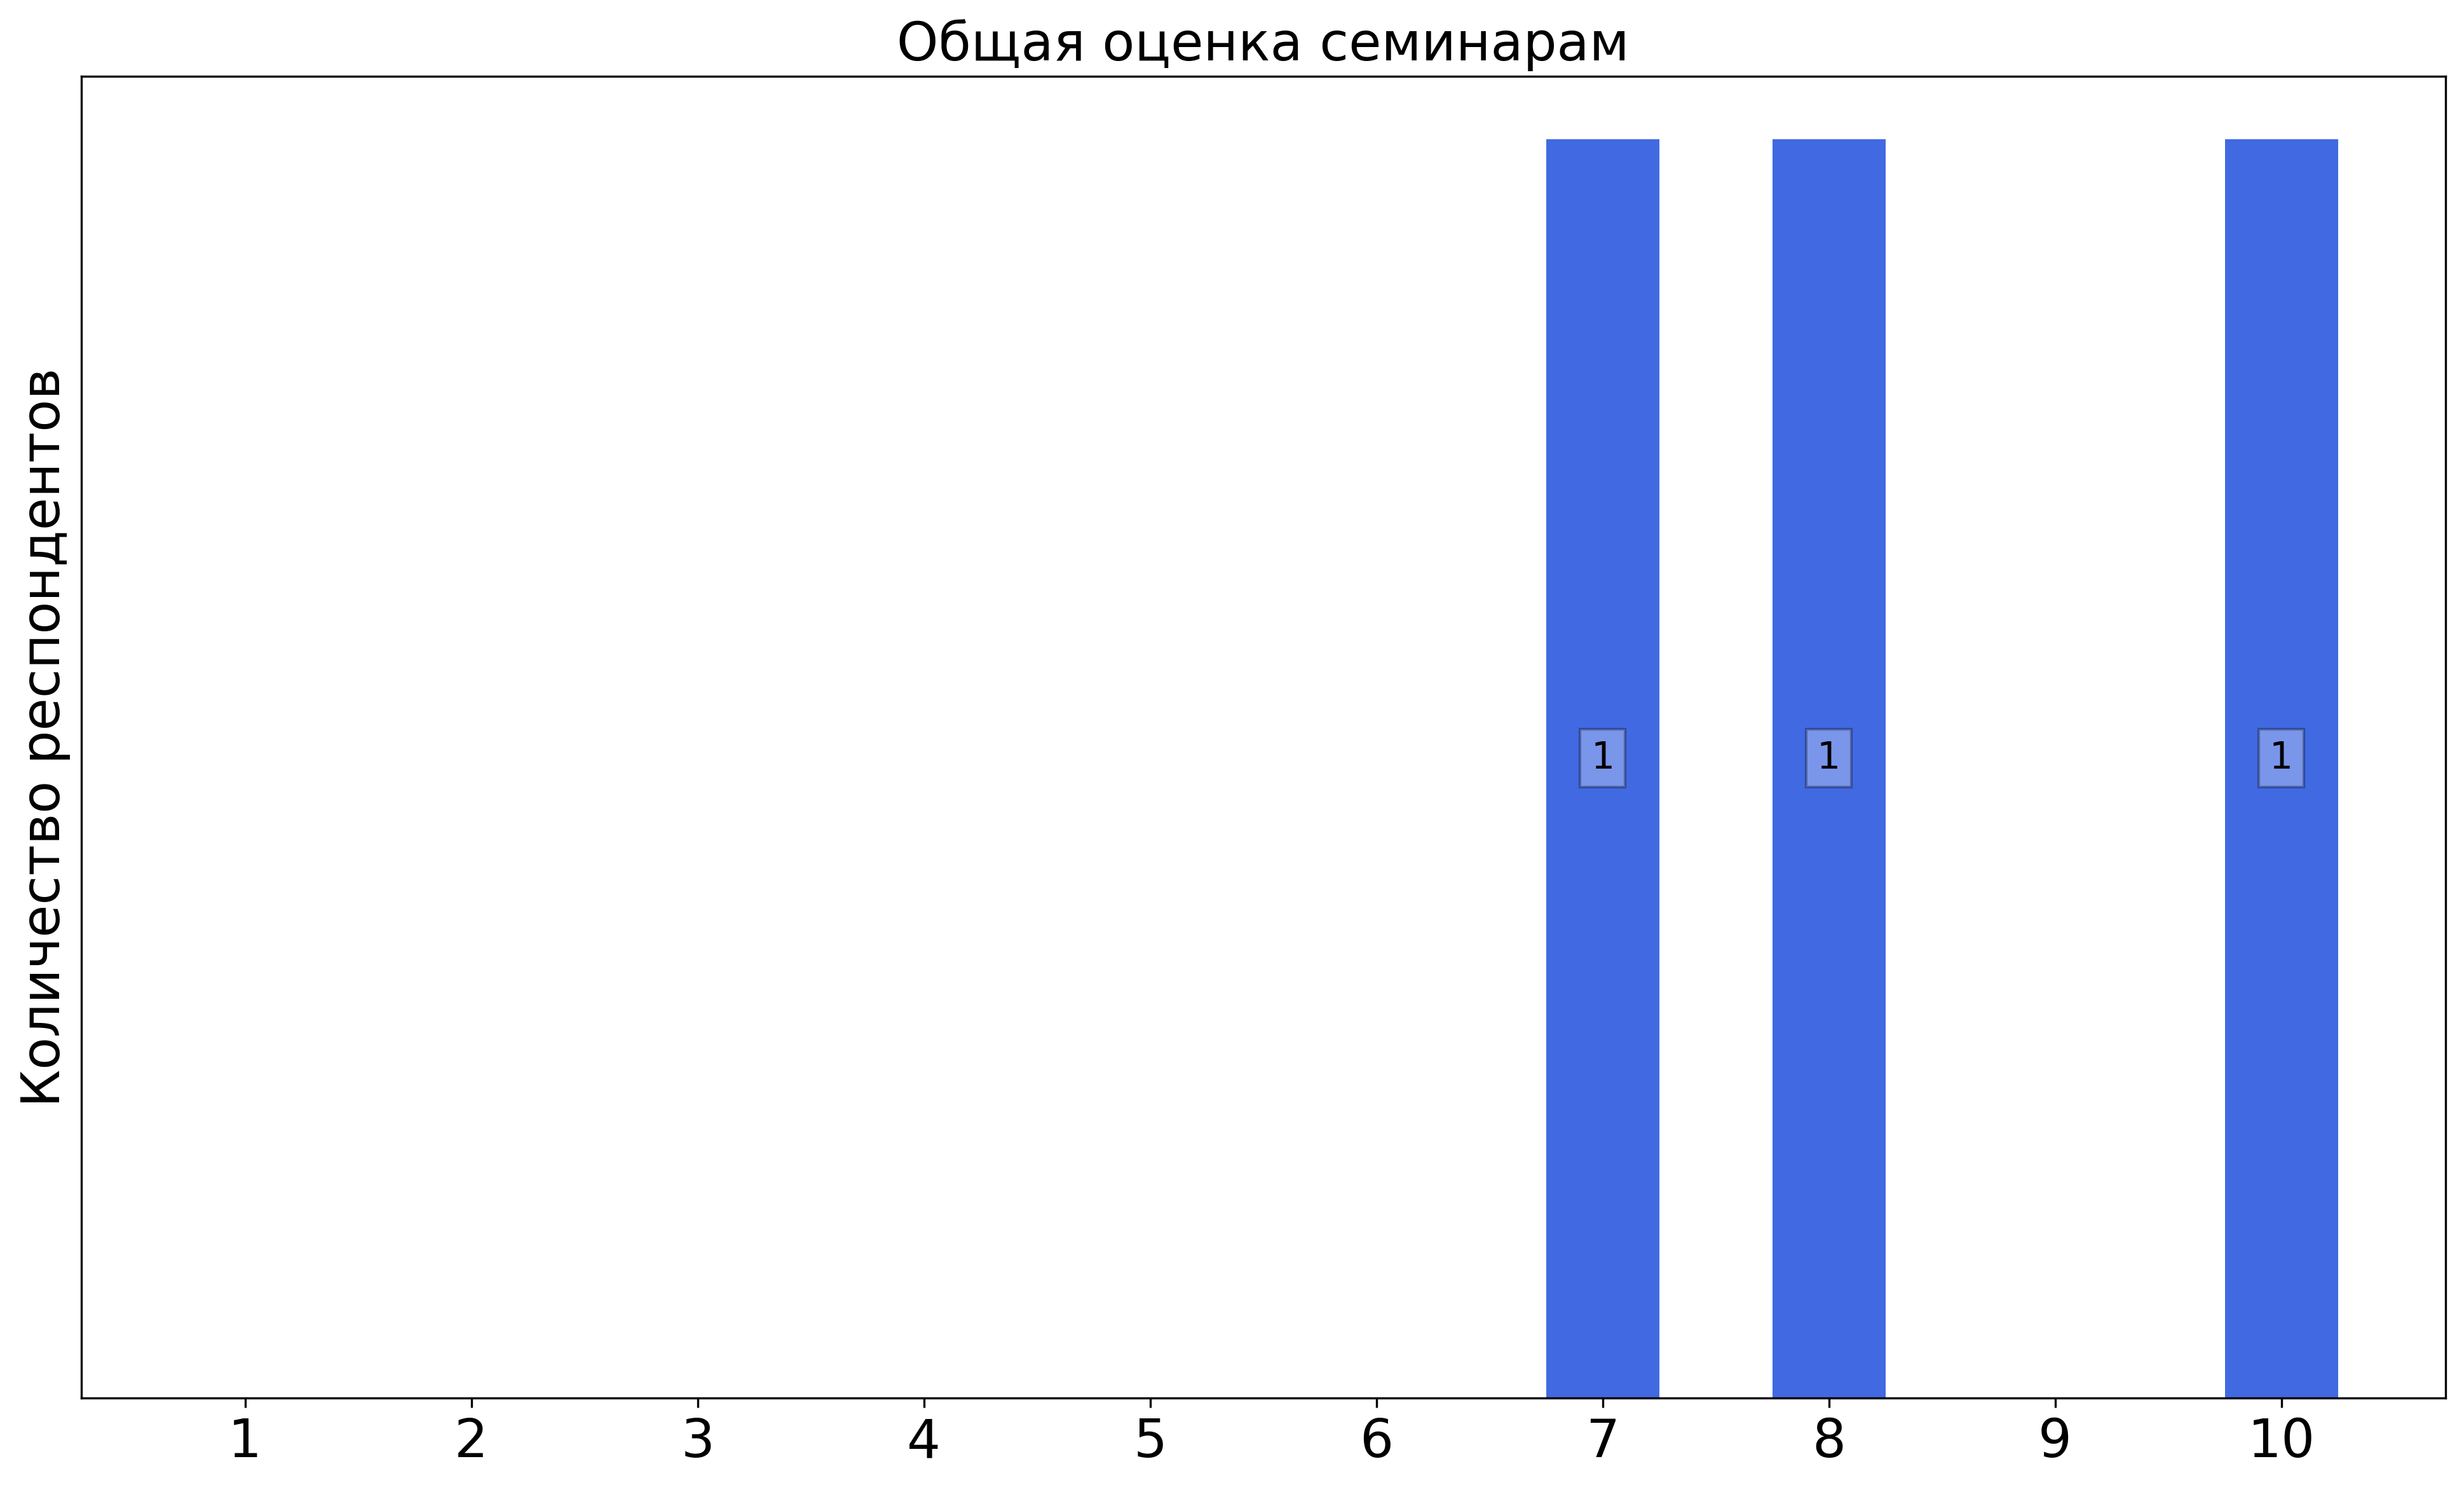
\includegraphics[width=\textwidth]{images/2 course/Общая физика - электричество и магнетизм/seminarists-marks-Овчинкин В.А.-3.png}
			\end{subfigure}	
			\caption{Оценки респондентов о качестве преподавания семинаров}
		\end{figure}


	\subsubsection{Отзыв студентов о семинарах. Семинарист: Пауков М.И.}
		\begin{figure}[H]
			\centering
			\begin{subfigure}[b]{0.45\textwidth}
				\centering
				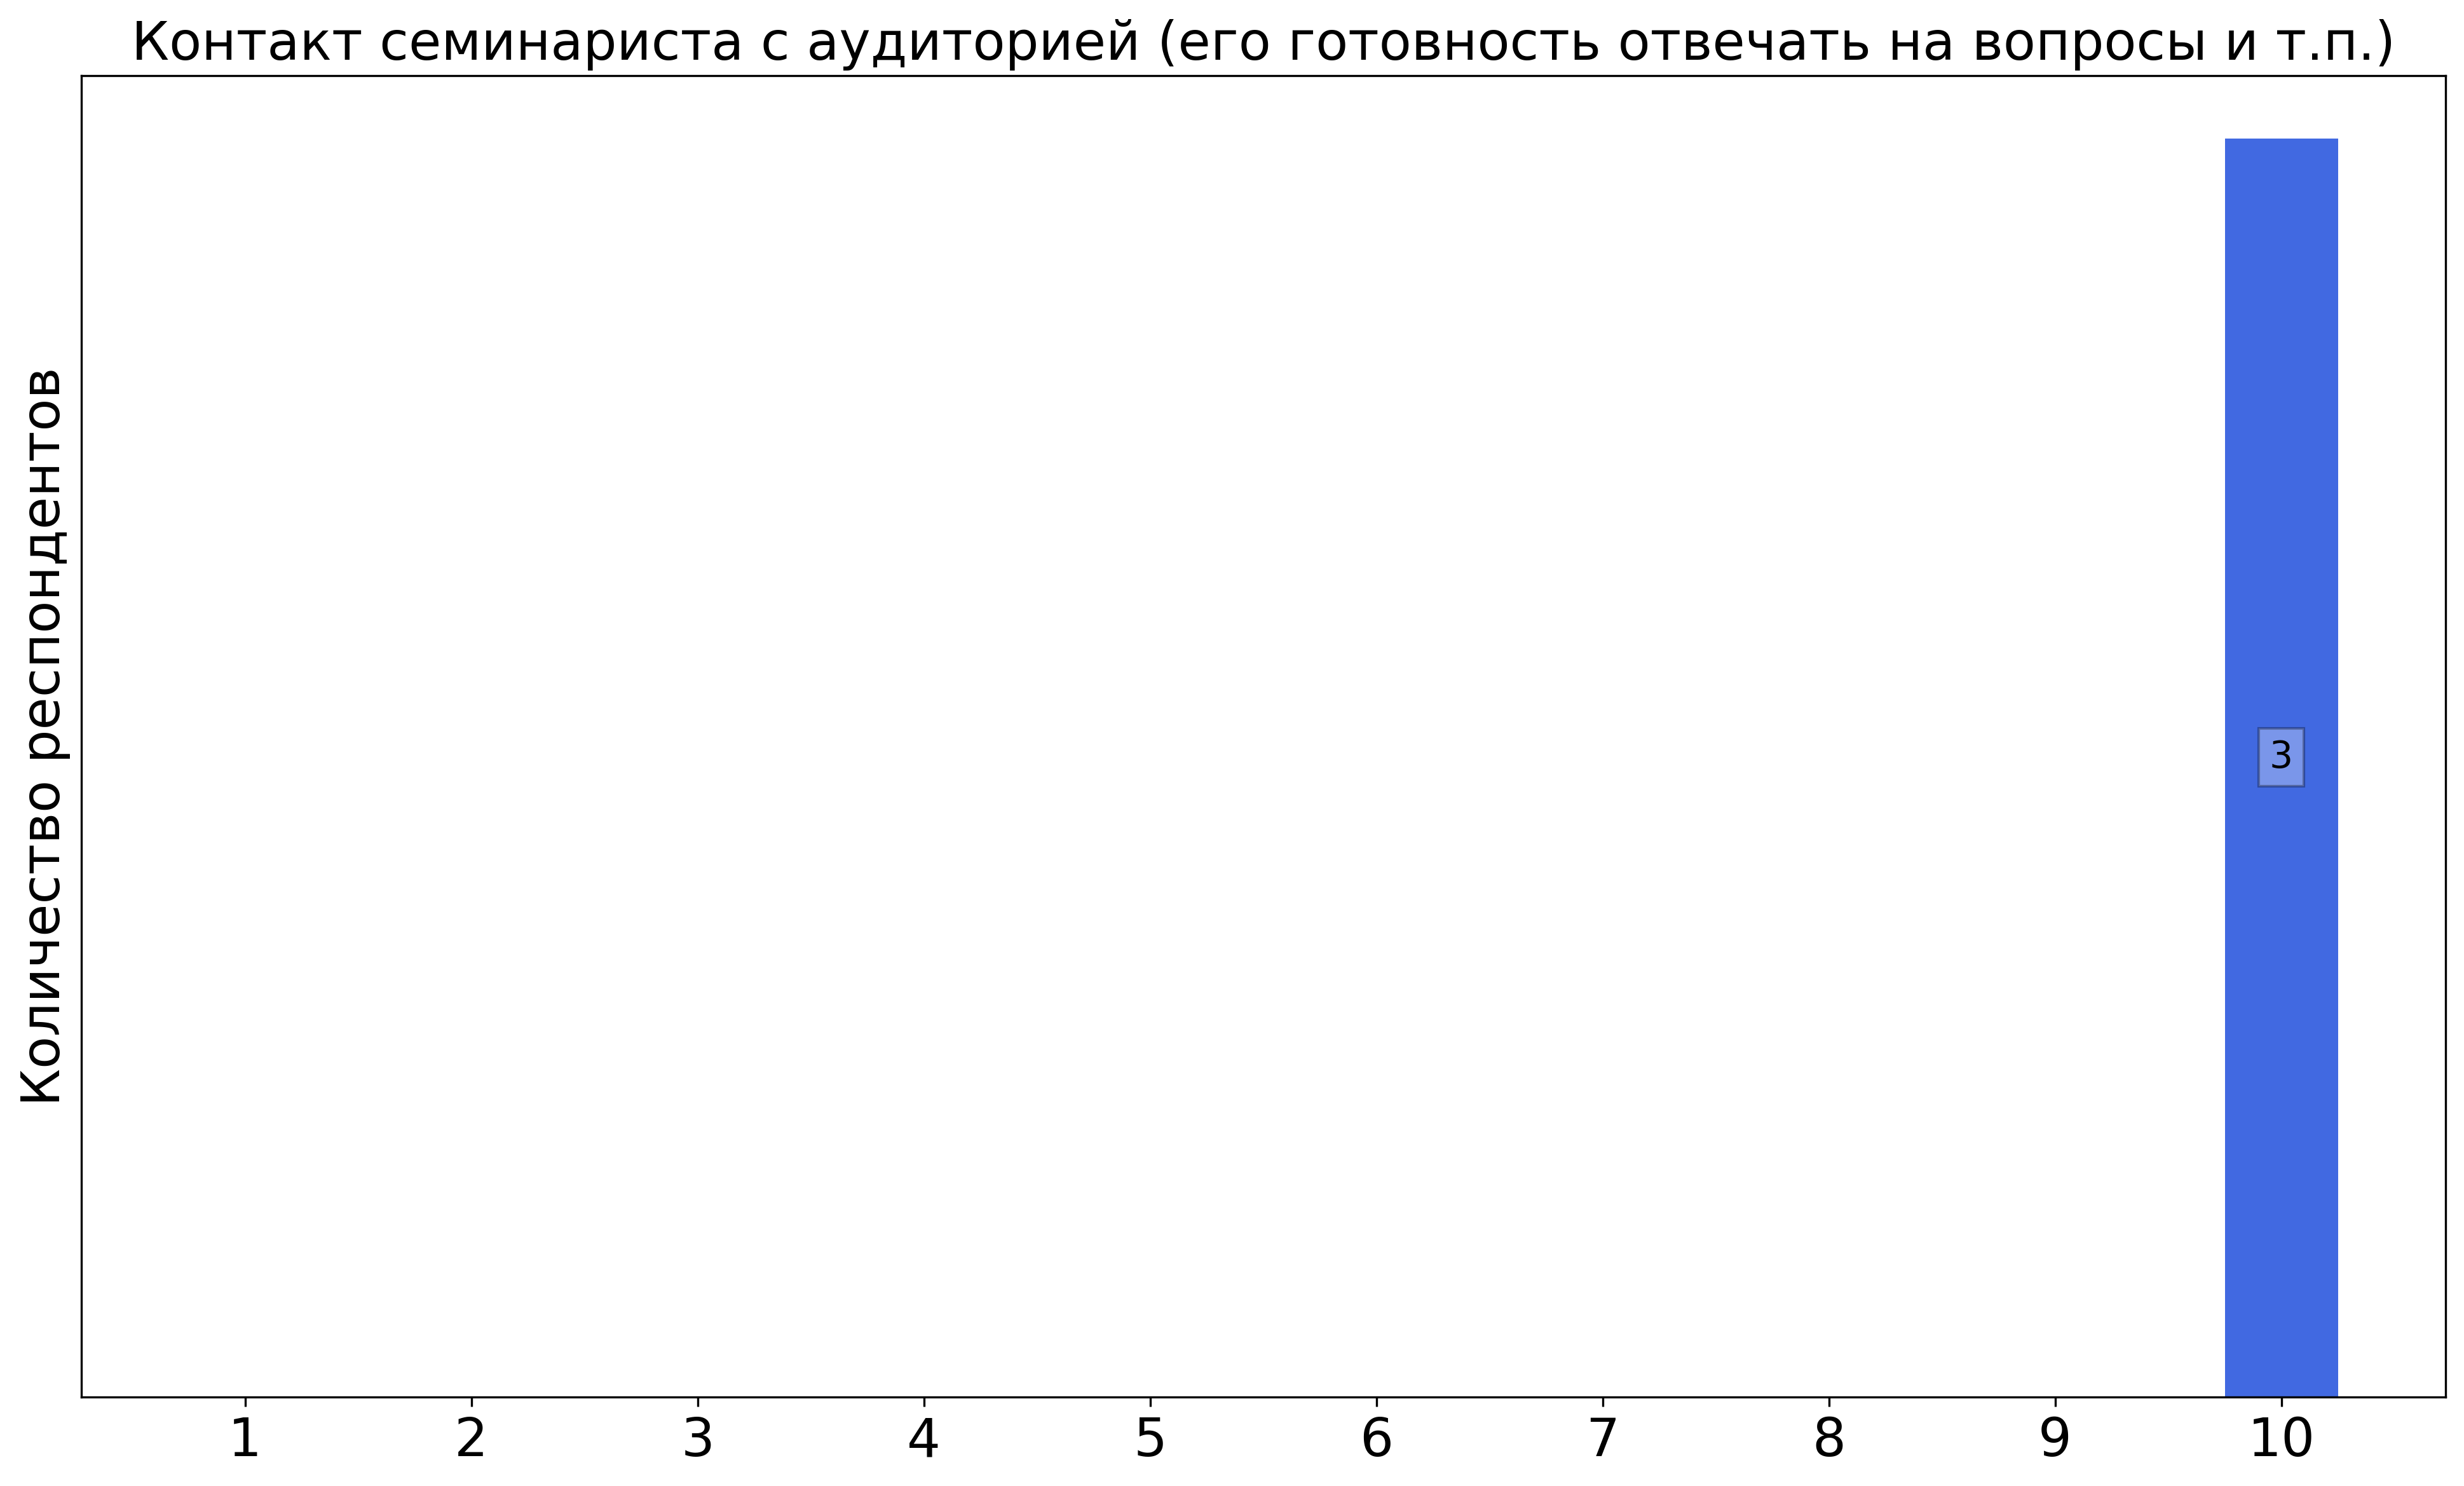
\includegraphics[width=\textwidth]{images/2 course/Общая физика - электричество и магнетизм/seminarists-marks-Пауков М.И.-0.png}
			\end{subfigure}
			\begin{subfigure}[b]{0.45\textwidth}
				\centering
				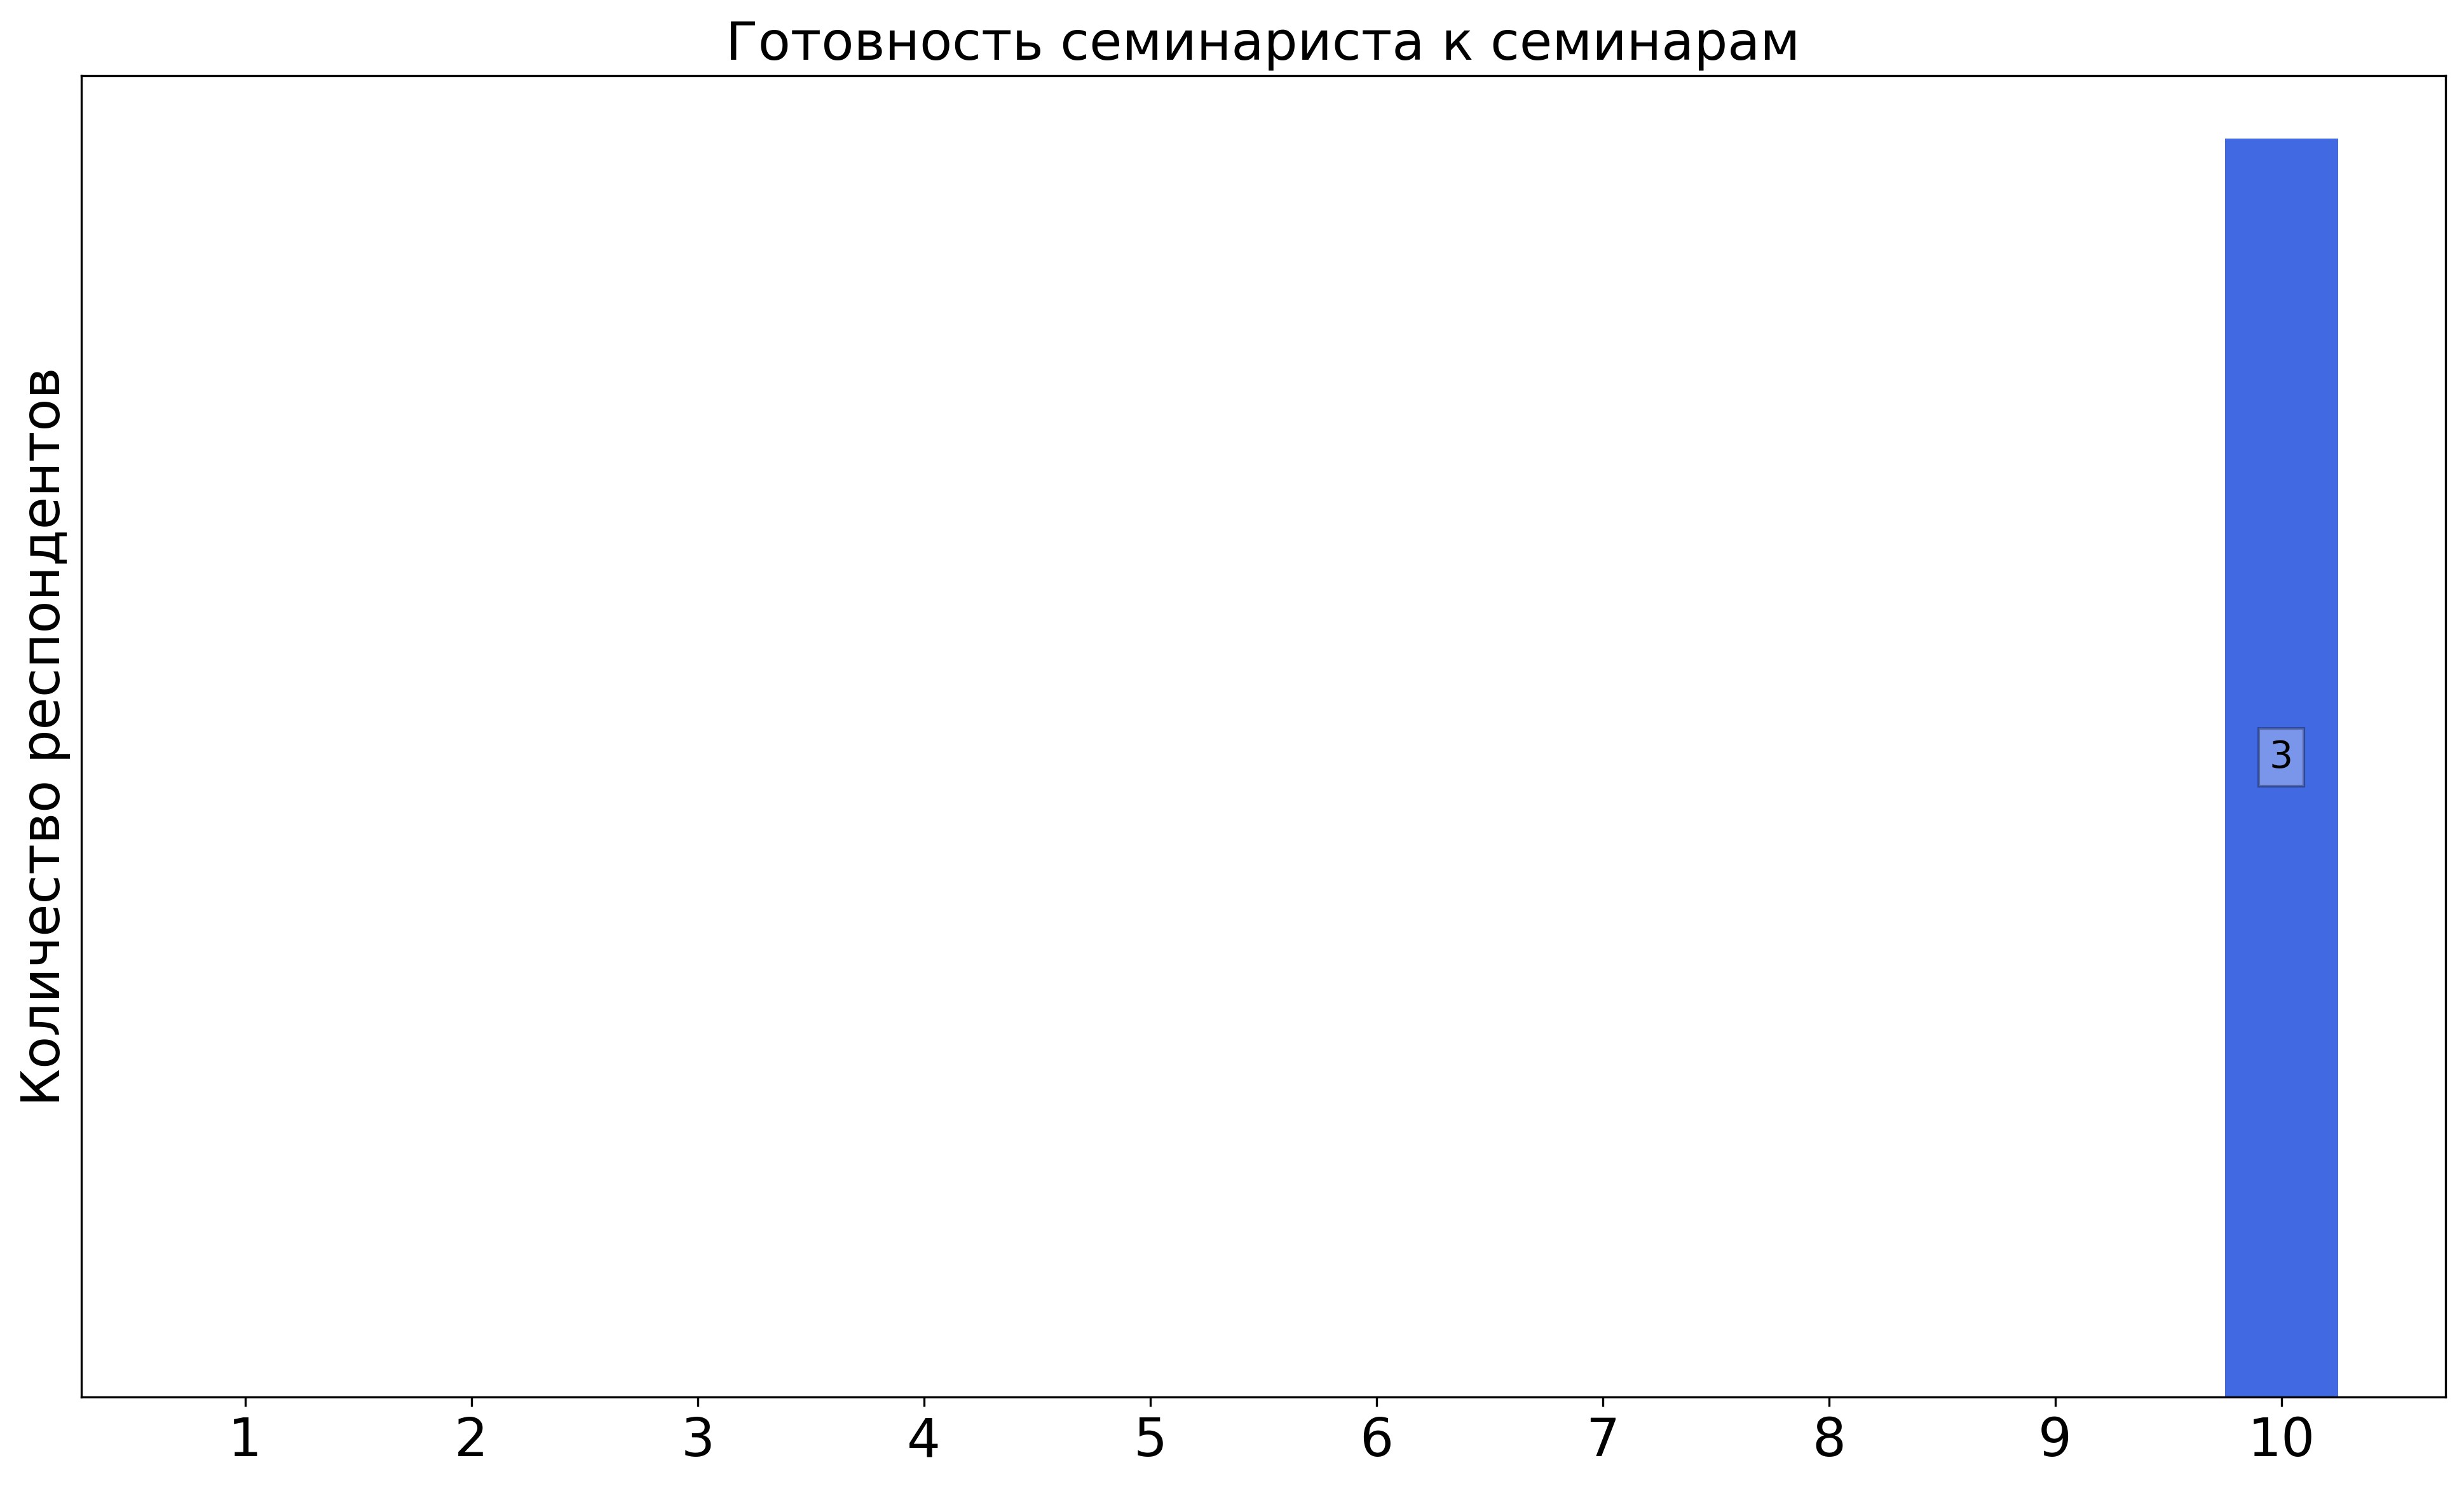
\includegraphics[width=\textwidth]{images/2 course/Общая физика - электричество и магнетизм/seminarists-marks-Пауков М.И.-1.png}
			\end{subfigure}
			\begin{subfigure}[b]{0.45\textwidth}
				\centering
				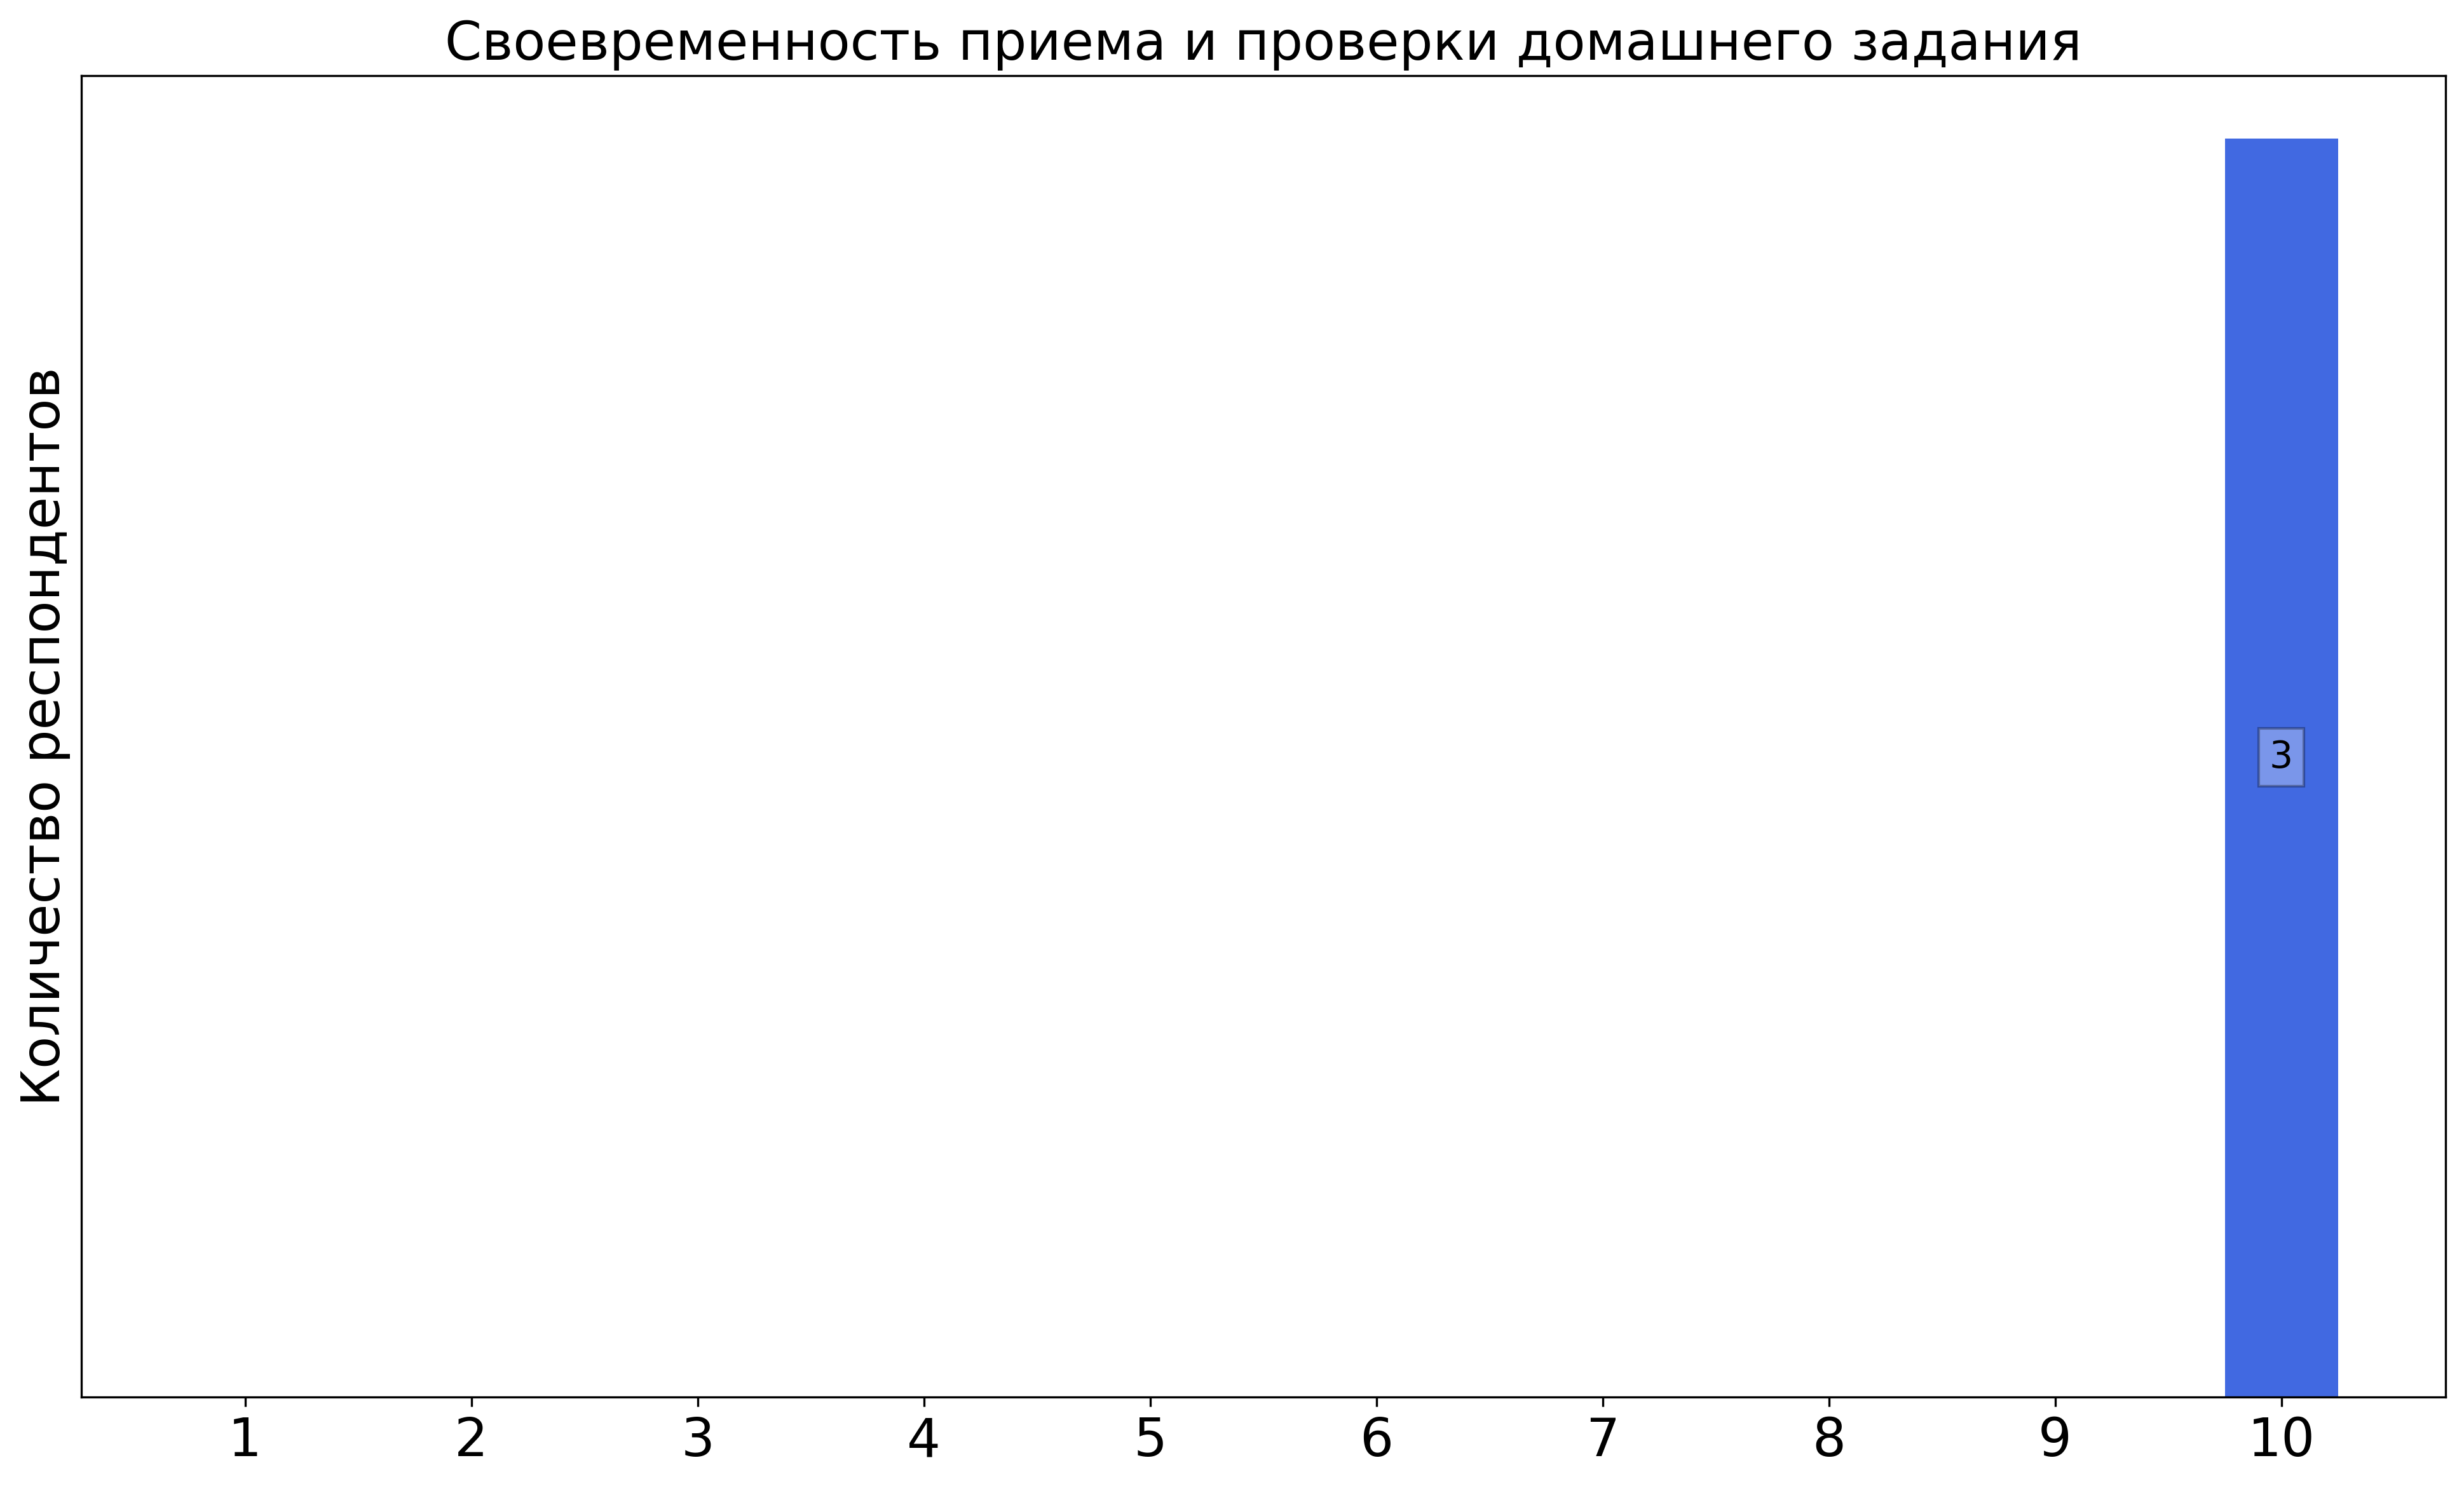
\includegraphics[width=\textwidth]{images/2 course/Общая физика - электричество и магнетизм/seminarists-marks-Пауков М.И.-2.png}
			\end{subfigure}
			\begin{subfigure}[b]{0.45\textwidth}
				\centering
				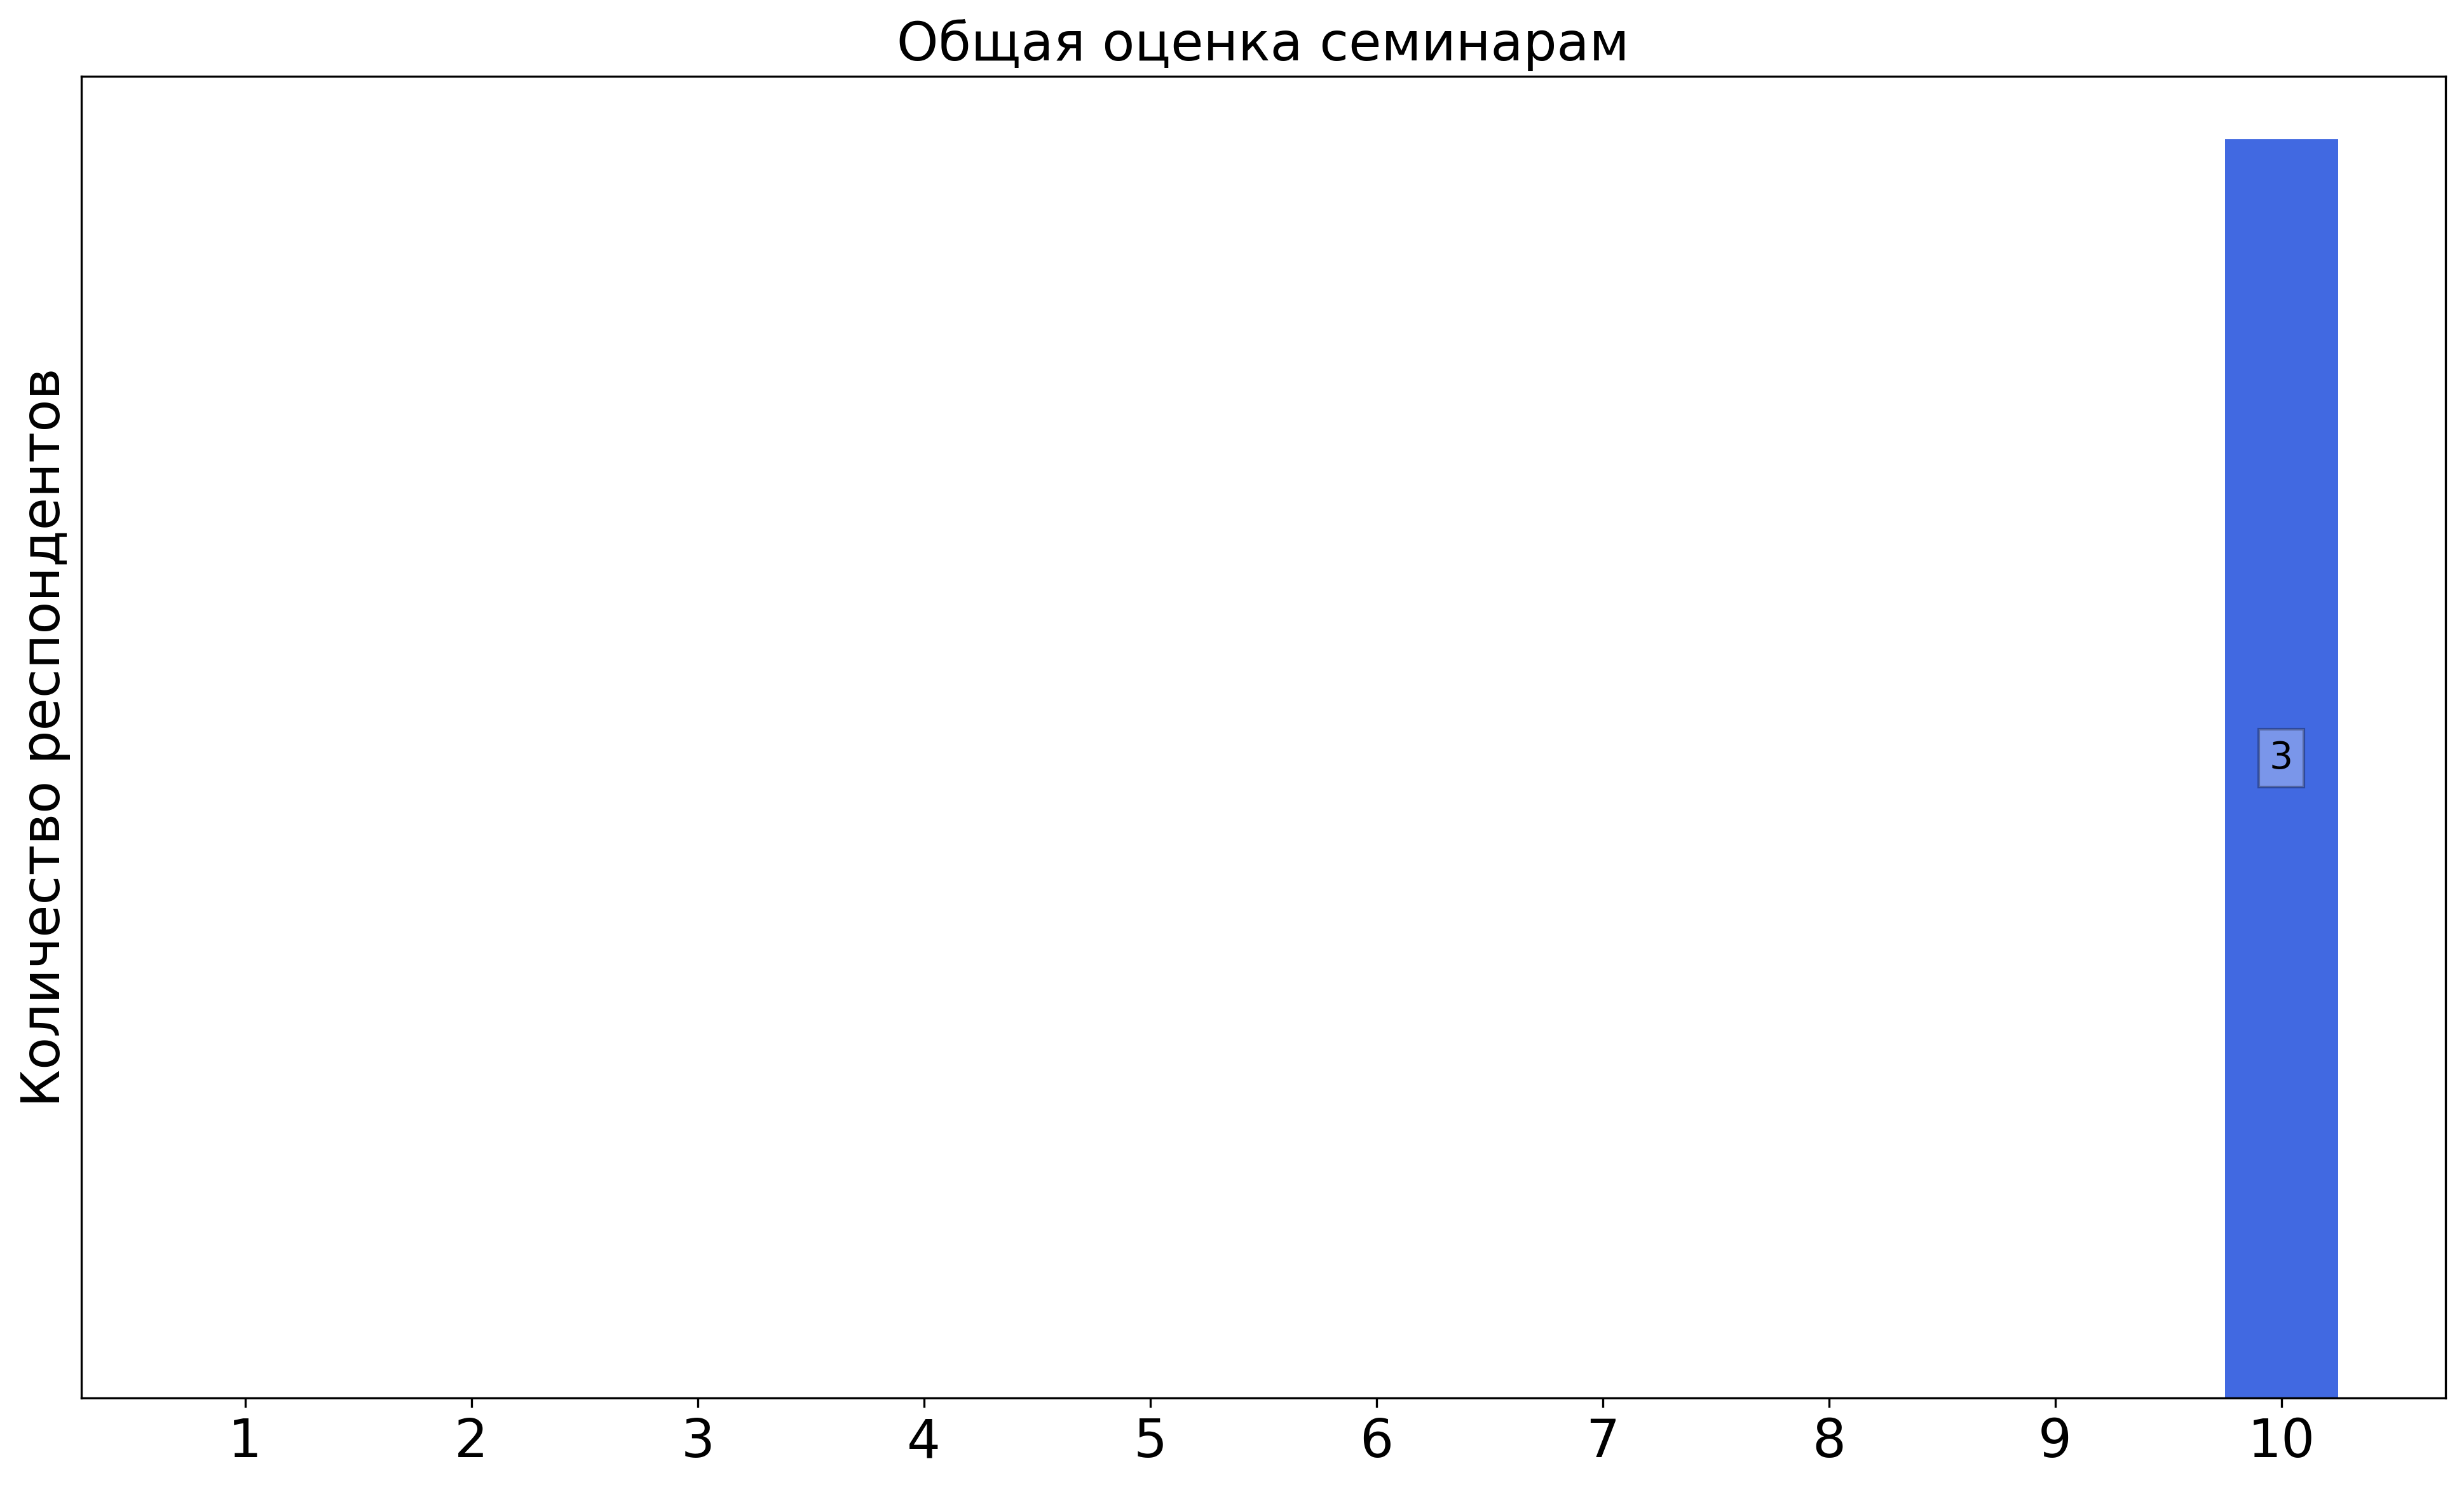
\includegraphics[width=\textwidth]{images/2 course/Общая физика - электричество и магнетизм/seminarists-marks-Пауков М.И.-3.png}
			\end{subfigure}	
			\caption{Оценки респондентов о качестве преподавания семинаров}
		\end{figure}

		\textbf{Комментарии студентов о семинаристе\protect\footnote{сохранены оригинальные орфография и пунктуация}}
			\begin{commentbox} 
				Максим Игоревич - лучший семинарист за все время обучения на фт, вместо обязательных 1,5 часов в неделю он тратил на нас 6+ часов, и объяснял все очень понятно. 
			\end{commentbox} 

		
	\subsubsection{Отзыв студентов о семинарах. Семинарист: Рыбакова А.К.}
		\begin{figure}[H]
			\centering
			\begin{subfigure}[b]{0.45\textwidth}
				\centering
				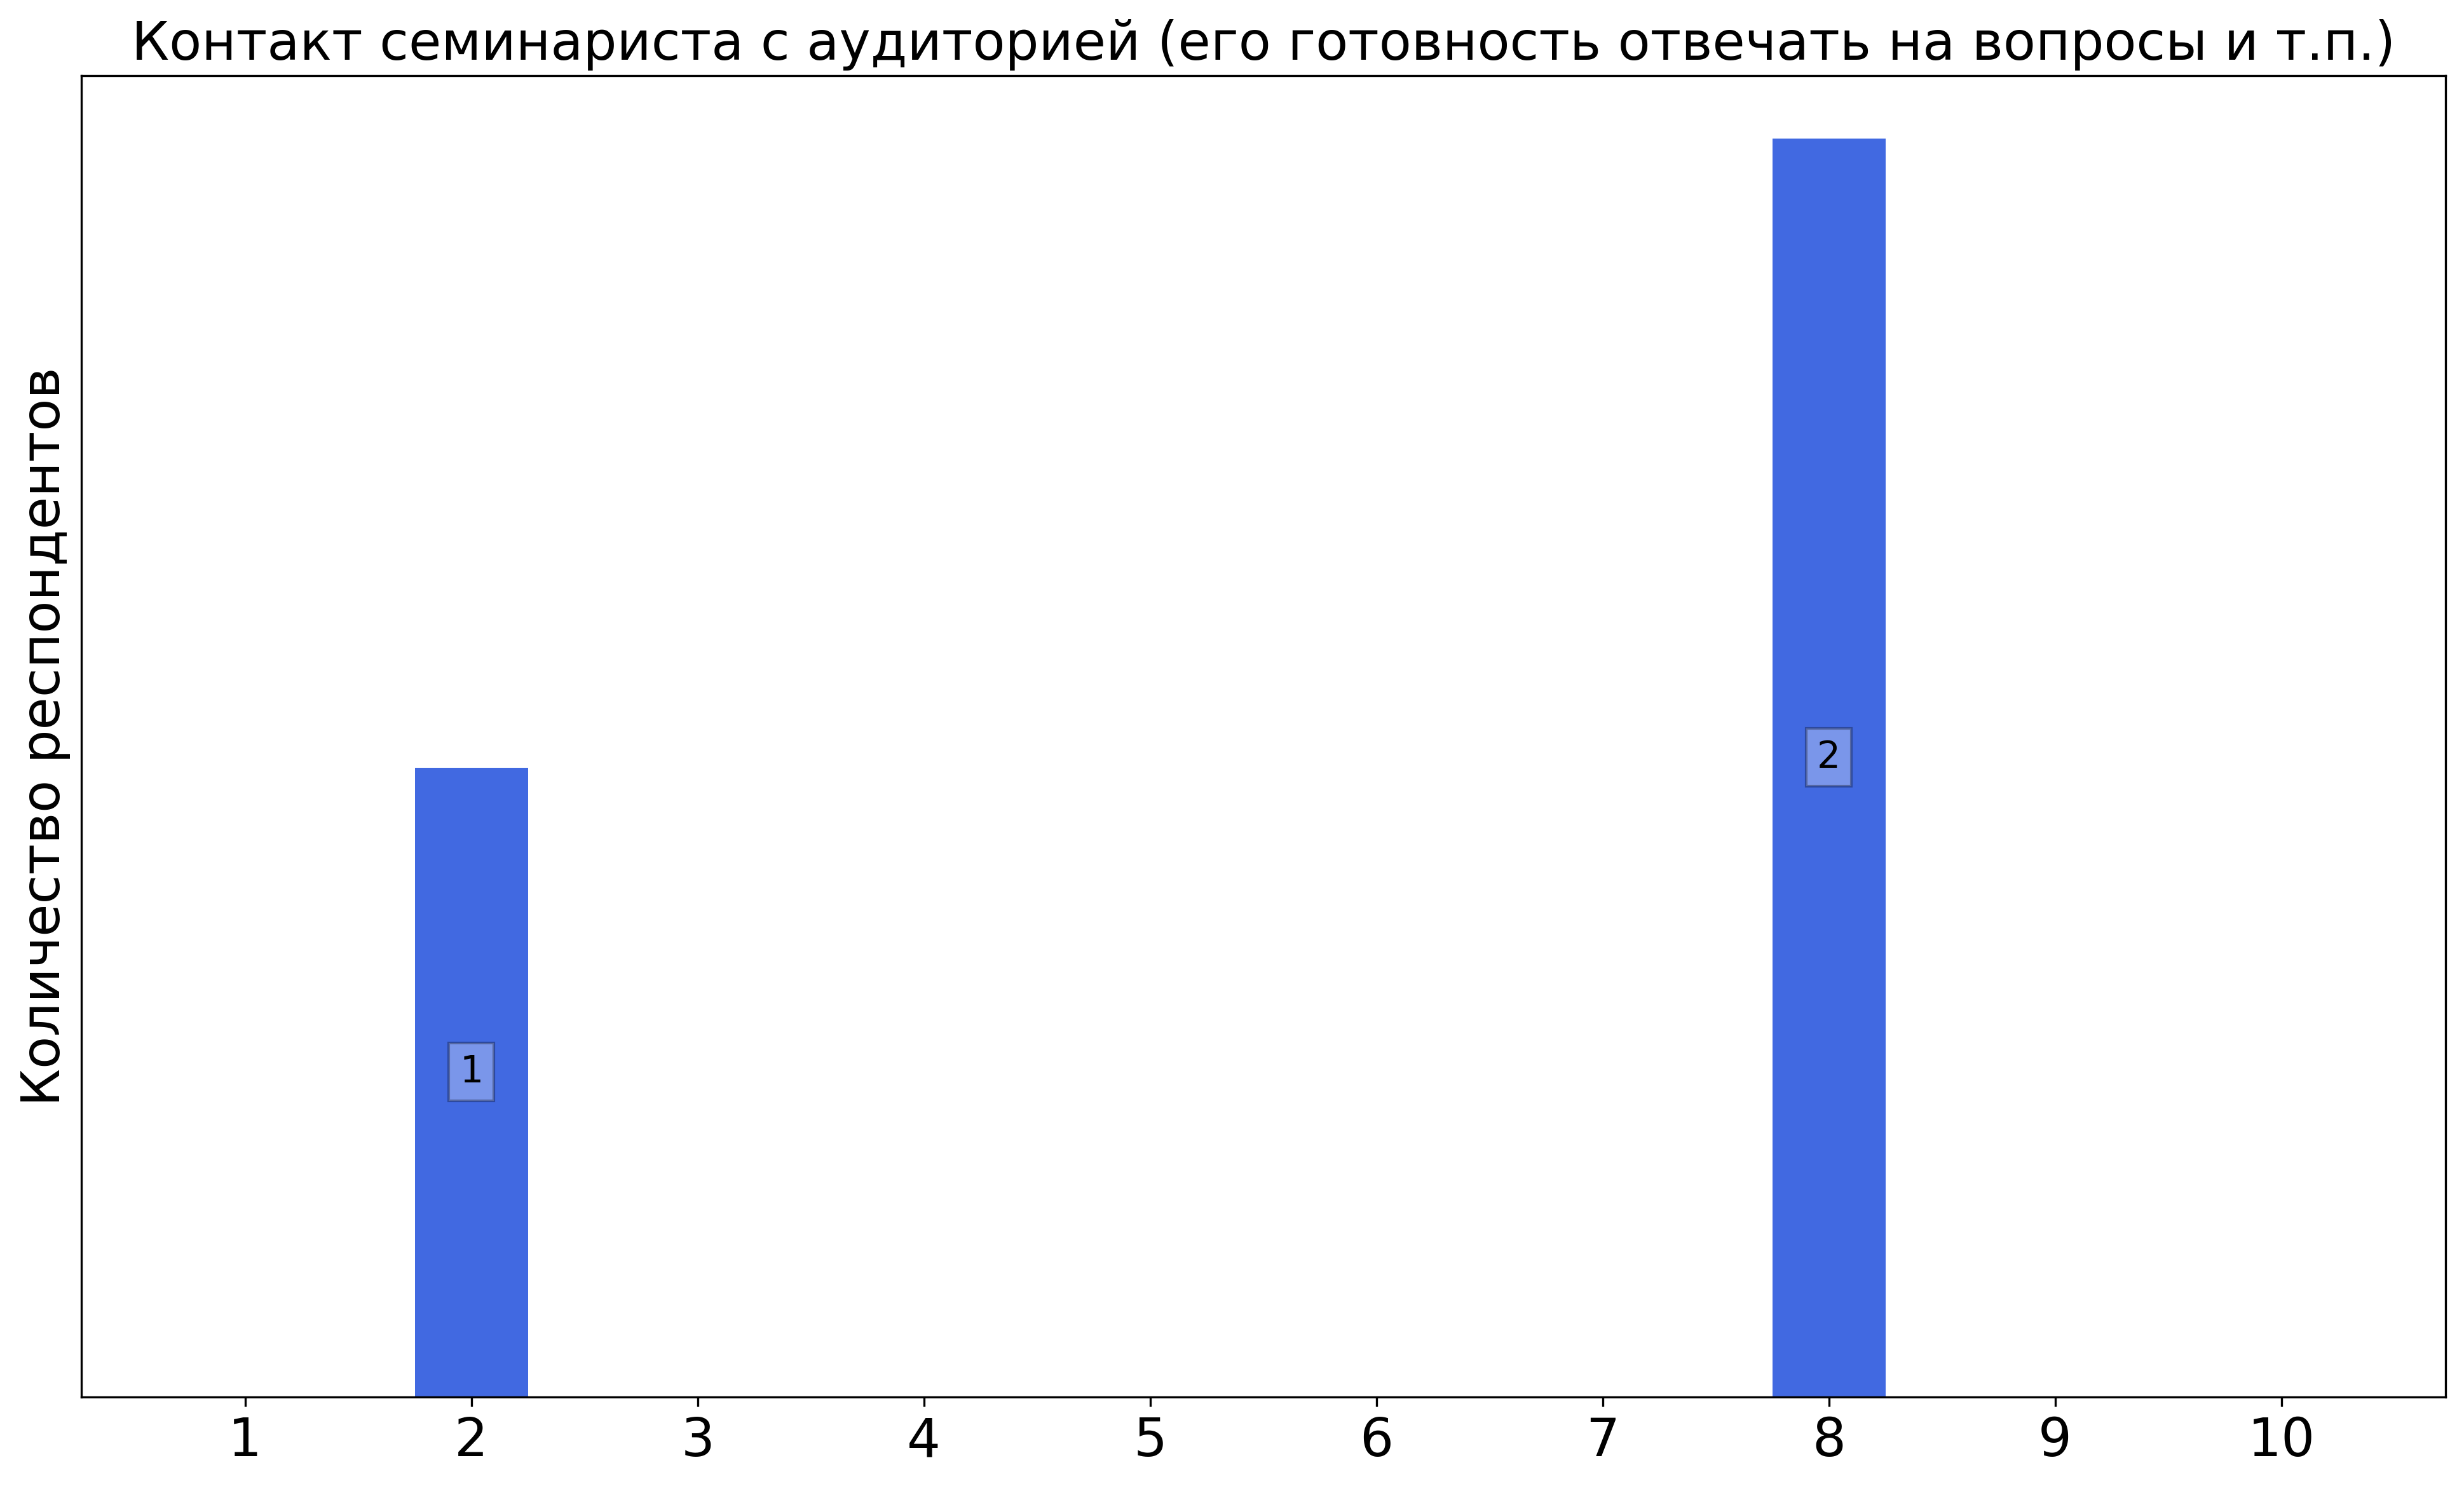
\includegraphics[width=\textwidth]{images/2 course/Общая физика - электричество и магнетизм/seminarists-marks-Рыбакова А.К.-0.png}
			\end{subfigure}
			\begin{subfigure}[b]{0.45\textwidth}
				\centering
				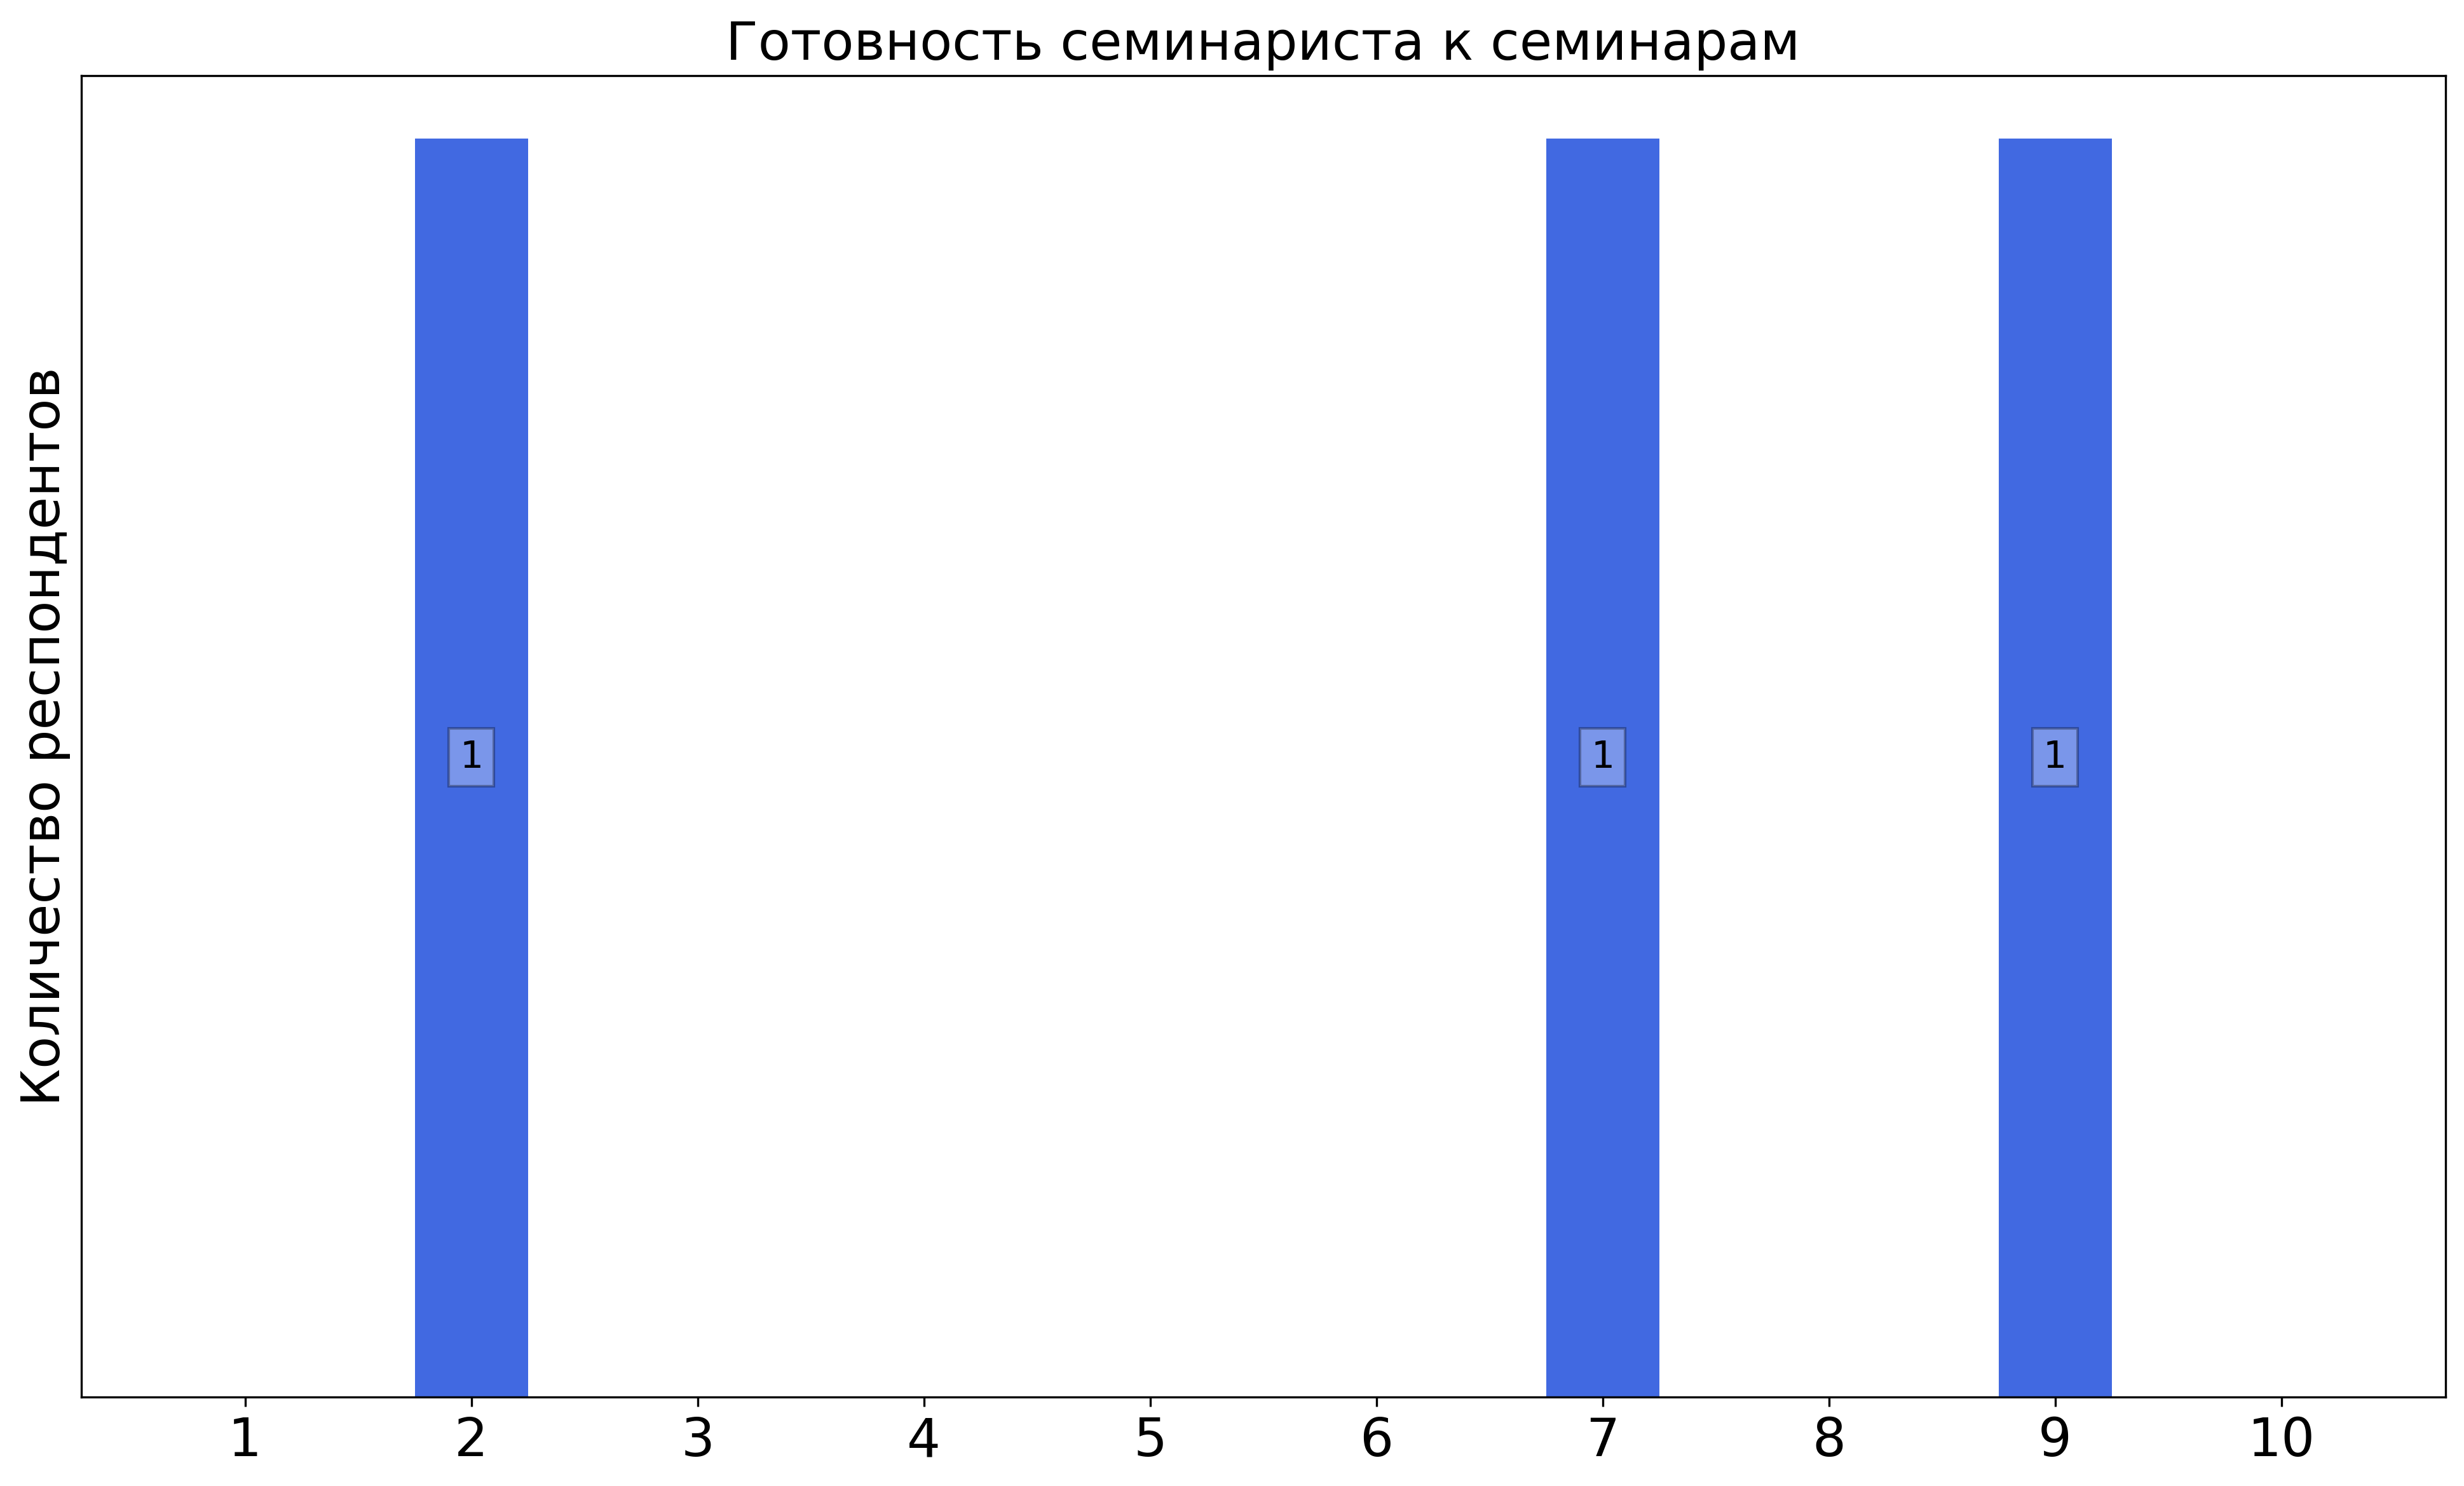
\includegraphics[width=\textwidth]{images/2 course/Общая физика - электричество и магнетизм/seminarists-marks-Рыбакова А.К.-1.png}
			\end{subfigure}
			\begin{subfigure}[b]{0.45\textwidth}
				\centering
				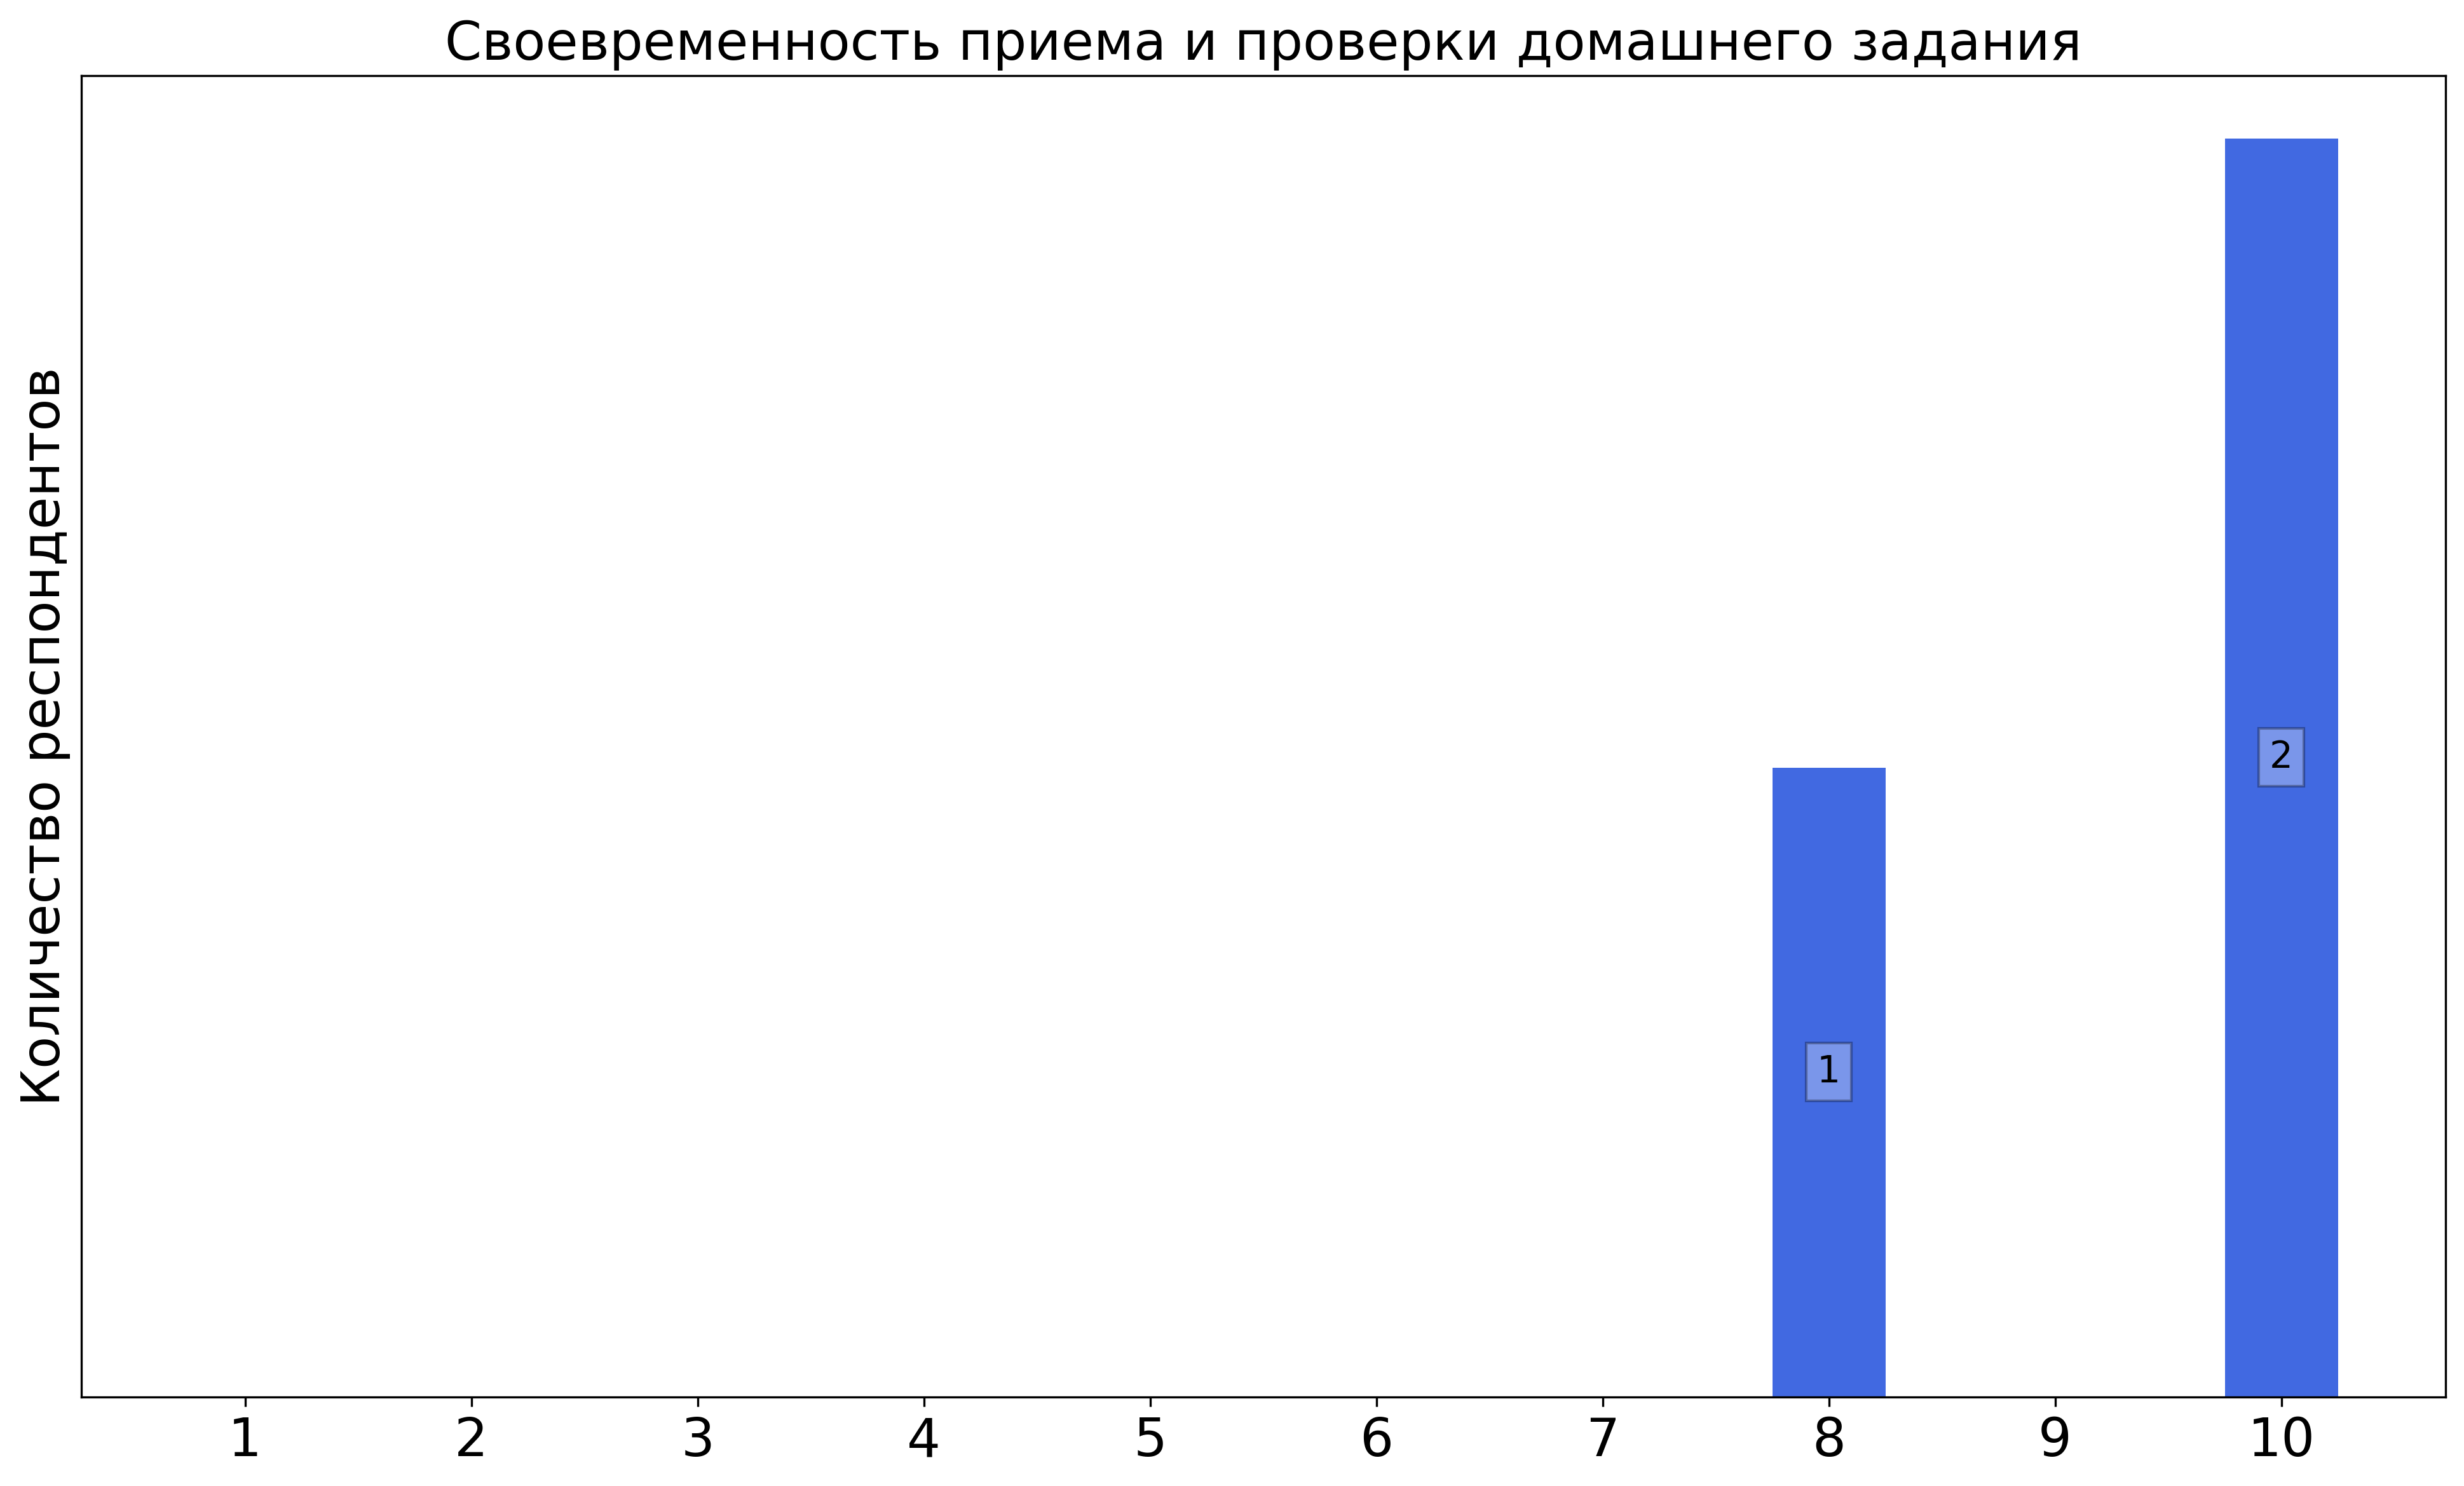
\includegraphics[width=\textwidth]{images/2 course/Общая физика - электричество и магнетизм/seminarists-marks-Рыбакова А.К.-2.png}
			\end{subfigure}
			\begin{subfigure}[b]{0.45\textwidth}
				\centering
				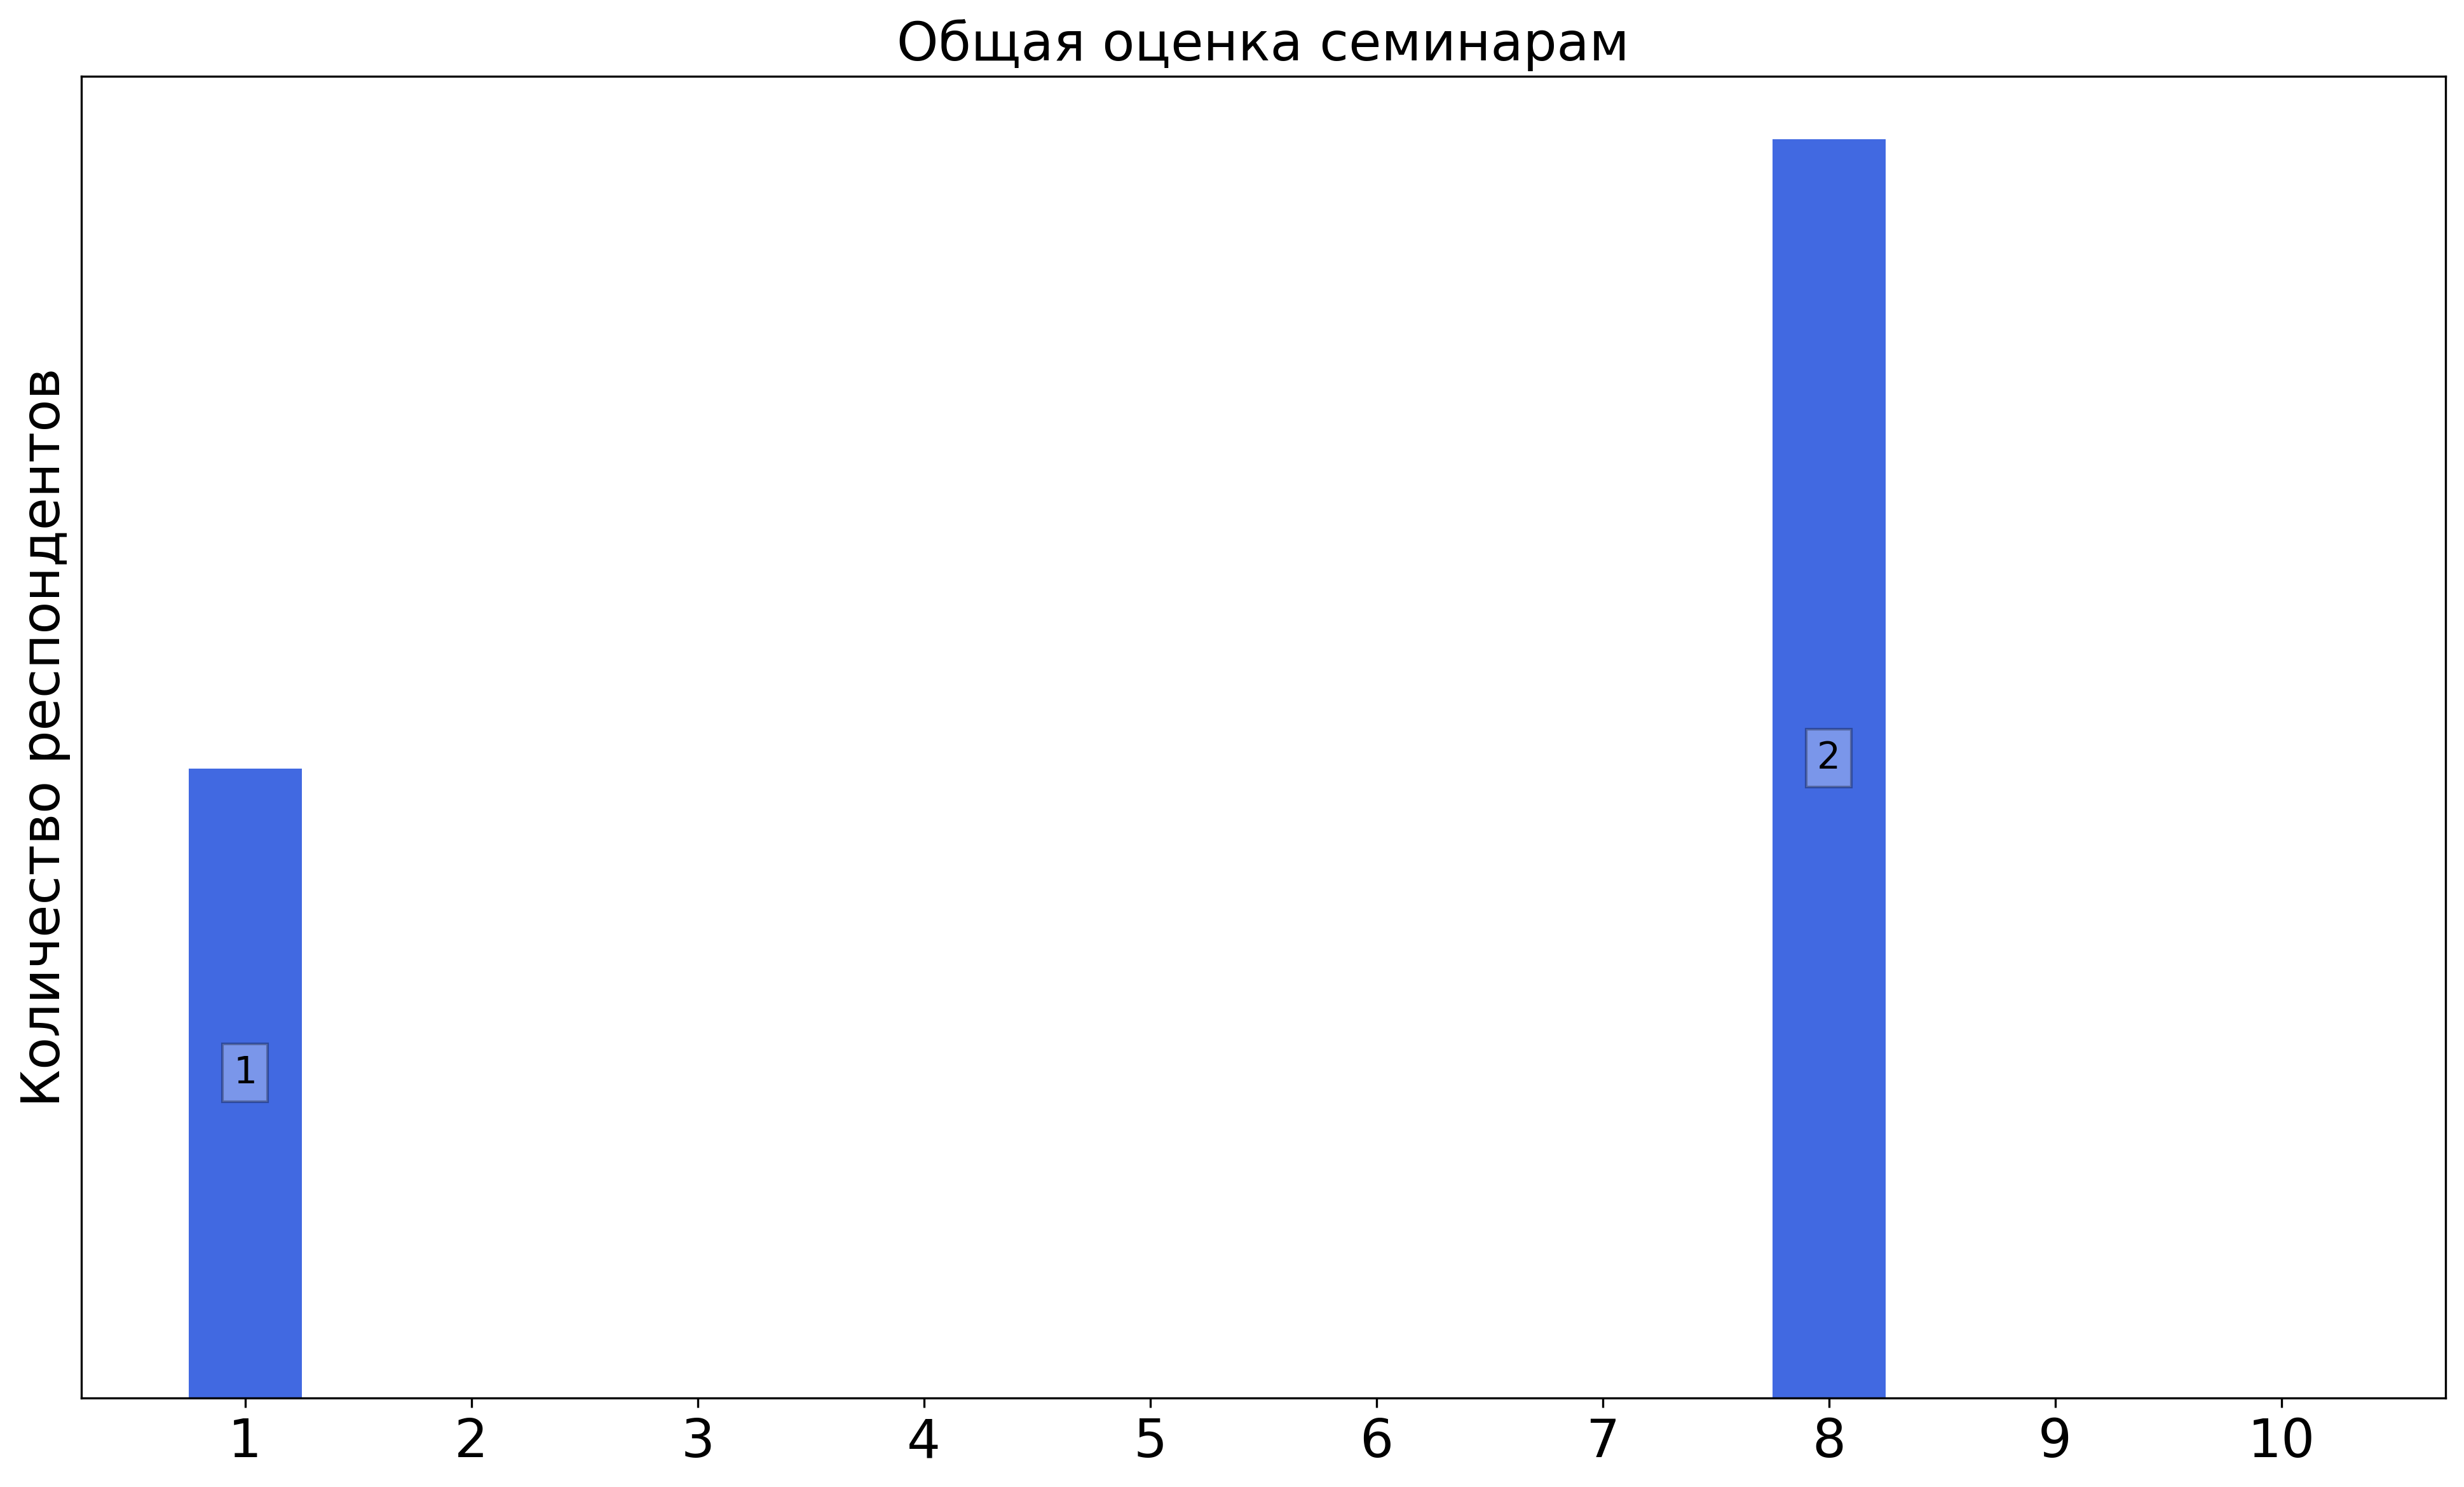
\includegraphics[width=\textwidth]{images/2 course/Общая физика - электричество и магнетизм/seminarists-marks-Рыбакова А.К.-3.png}
			\end{subfigure}	
			\caption{Оценки респондентов о качестве преподавания семинаров}
		\end{figure}


	\subsubsection{Отзыв студентов о семинарах. Семинарист: Седельников Е.В.}
		\begin{figure}[H]
			\centering
			\begin{subfigure}[b]{0.45\textwidth}
				\centering
				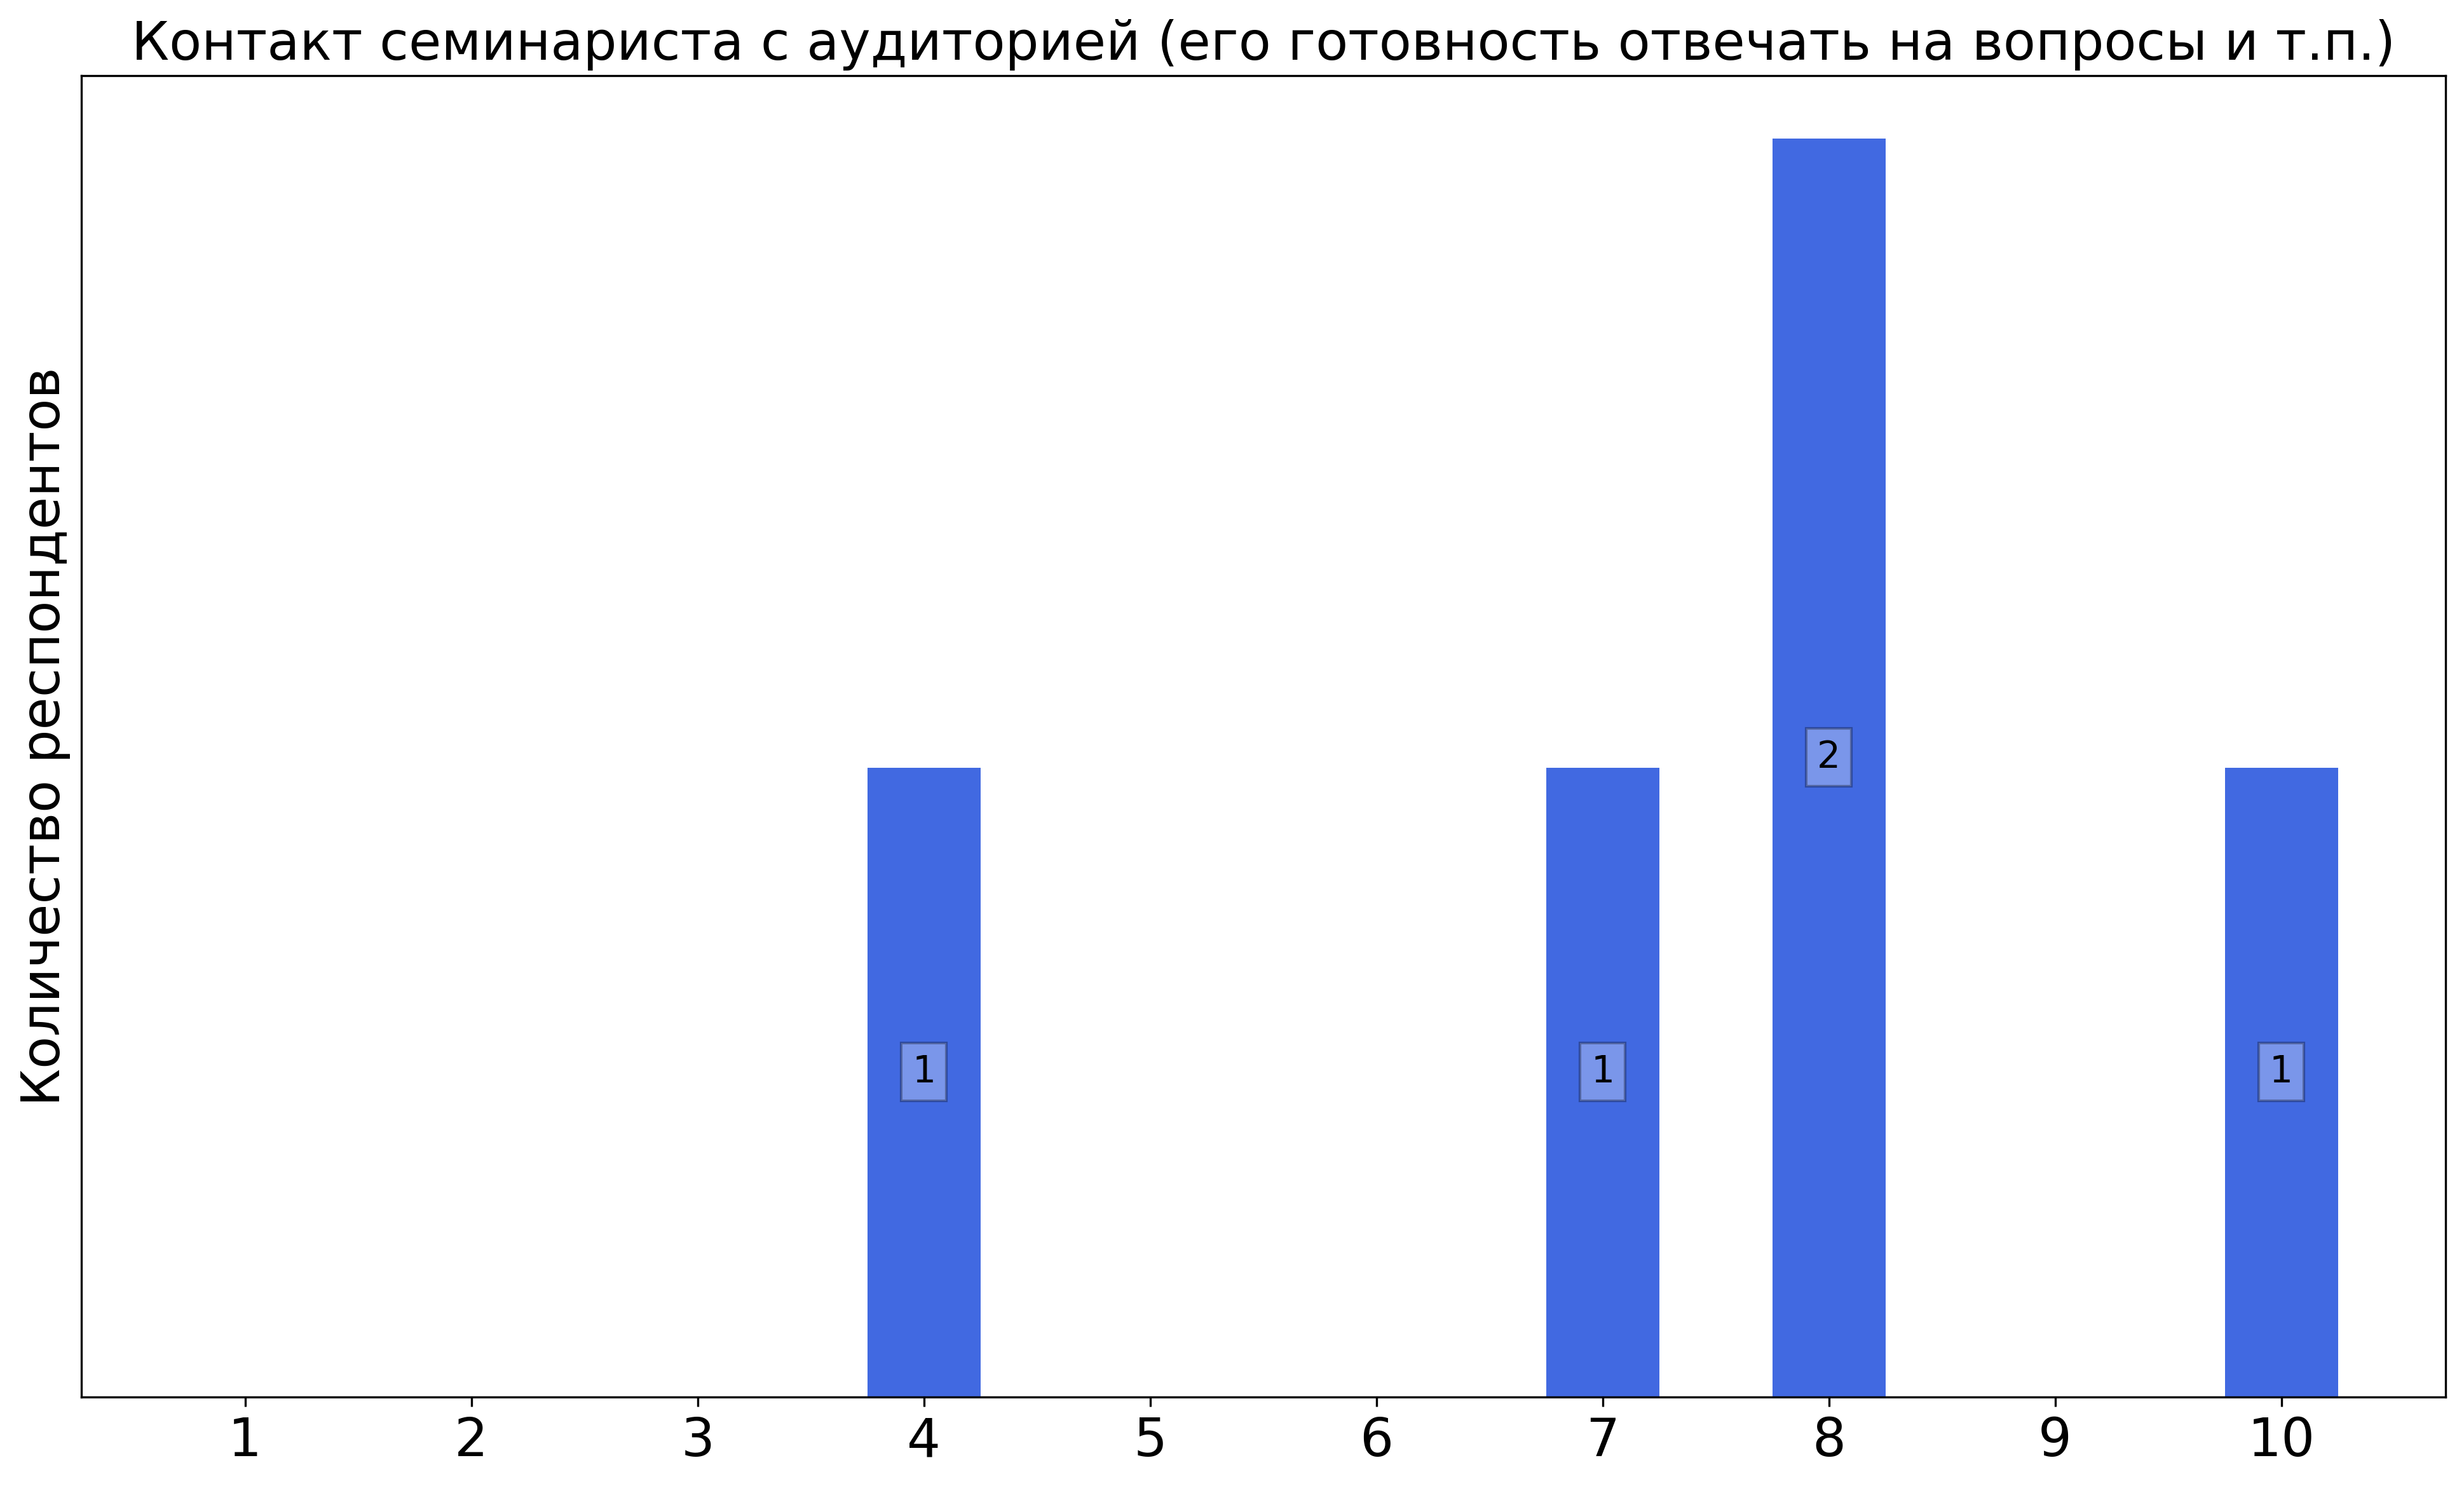
\includegraphics[width=\textwidth]{images/2 course/Общая физика - электричество и магнетизм/seminarists-marks-Седельников Е.В.-0.png}
			\end{subfigure}
			\begin{subfigure}[b]{0.45\textwidth}
				\centering
				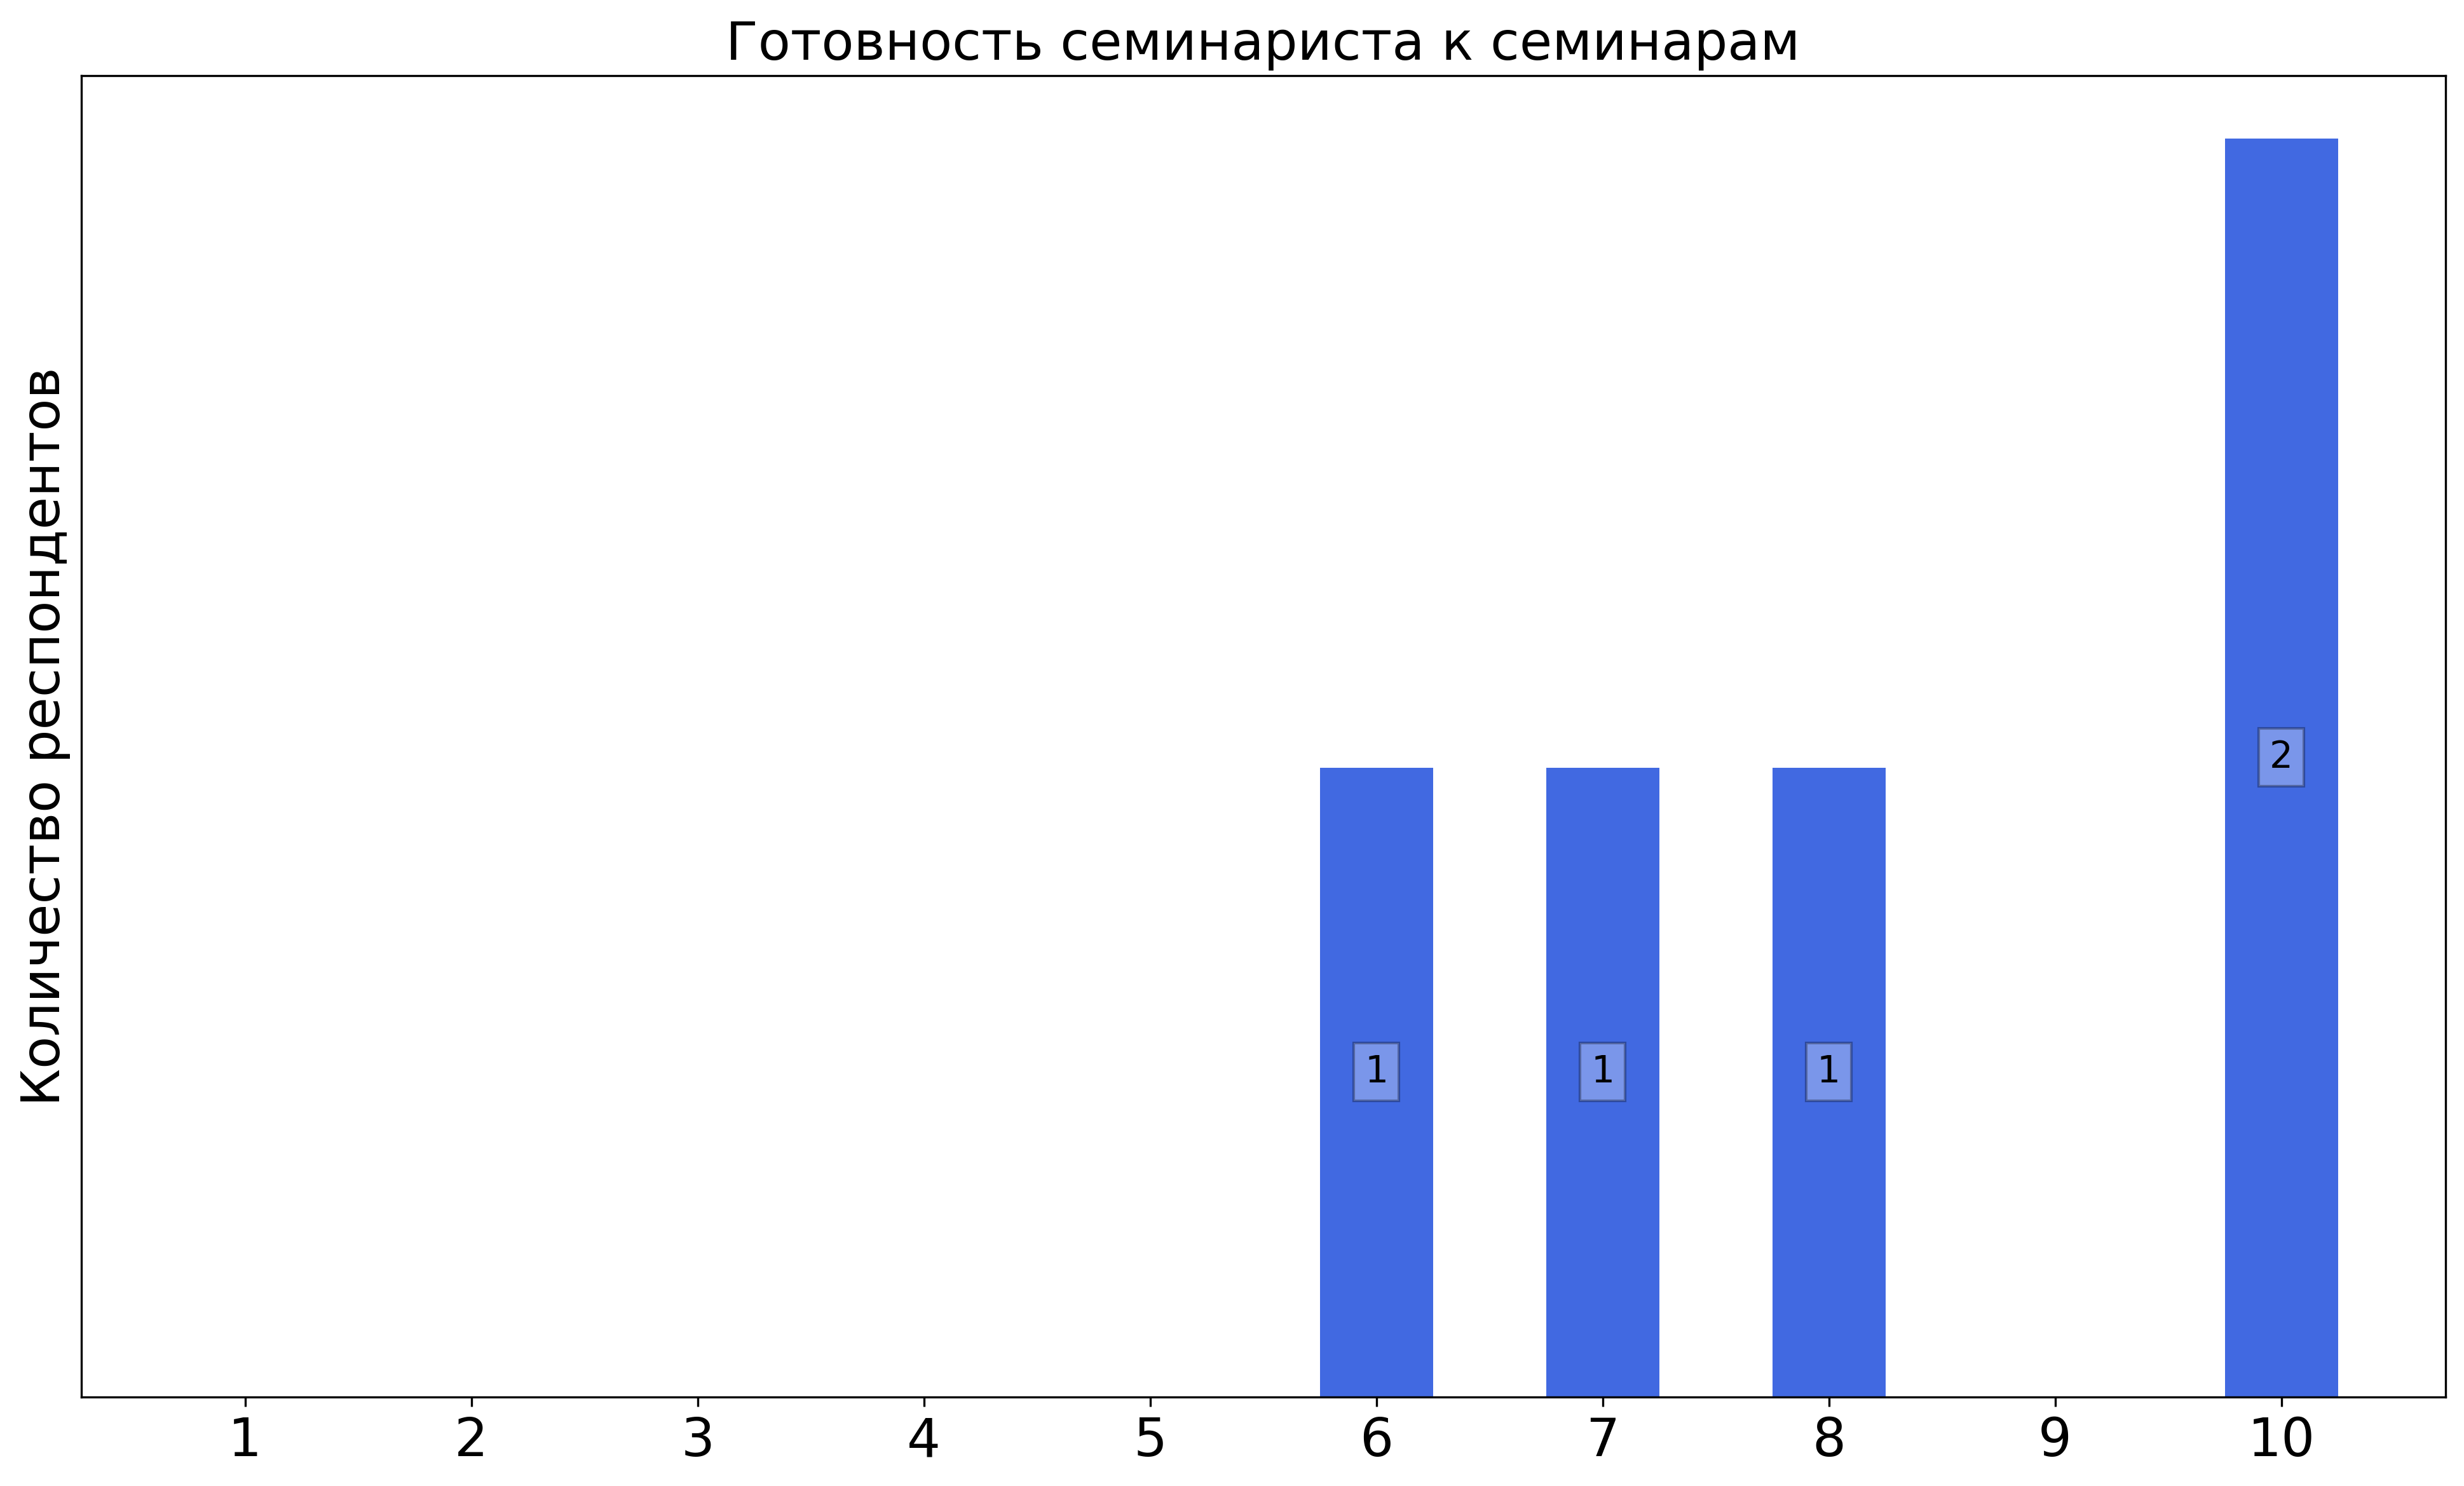
\includegraphics[width=\textwidth]{images/2 course/Общая физика - электричество и магнетизм/seminarists-marks-Седельников Е.В.-1.png}
			\end{subfigure}
			\begin{subfigure}[b]{0.45\textwidth}
				\centering
				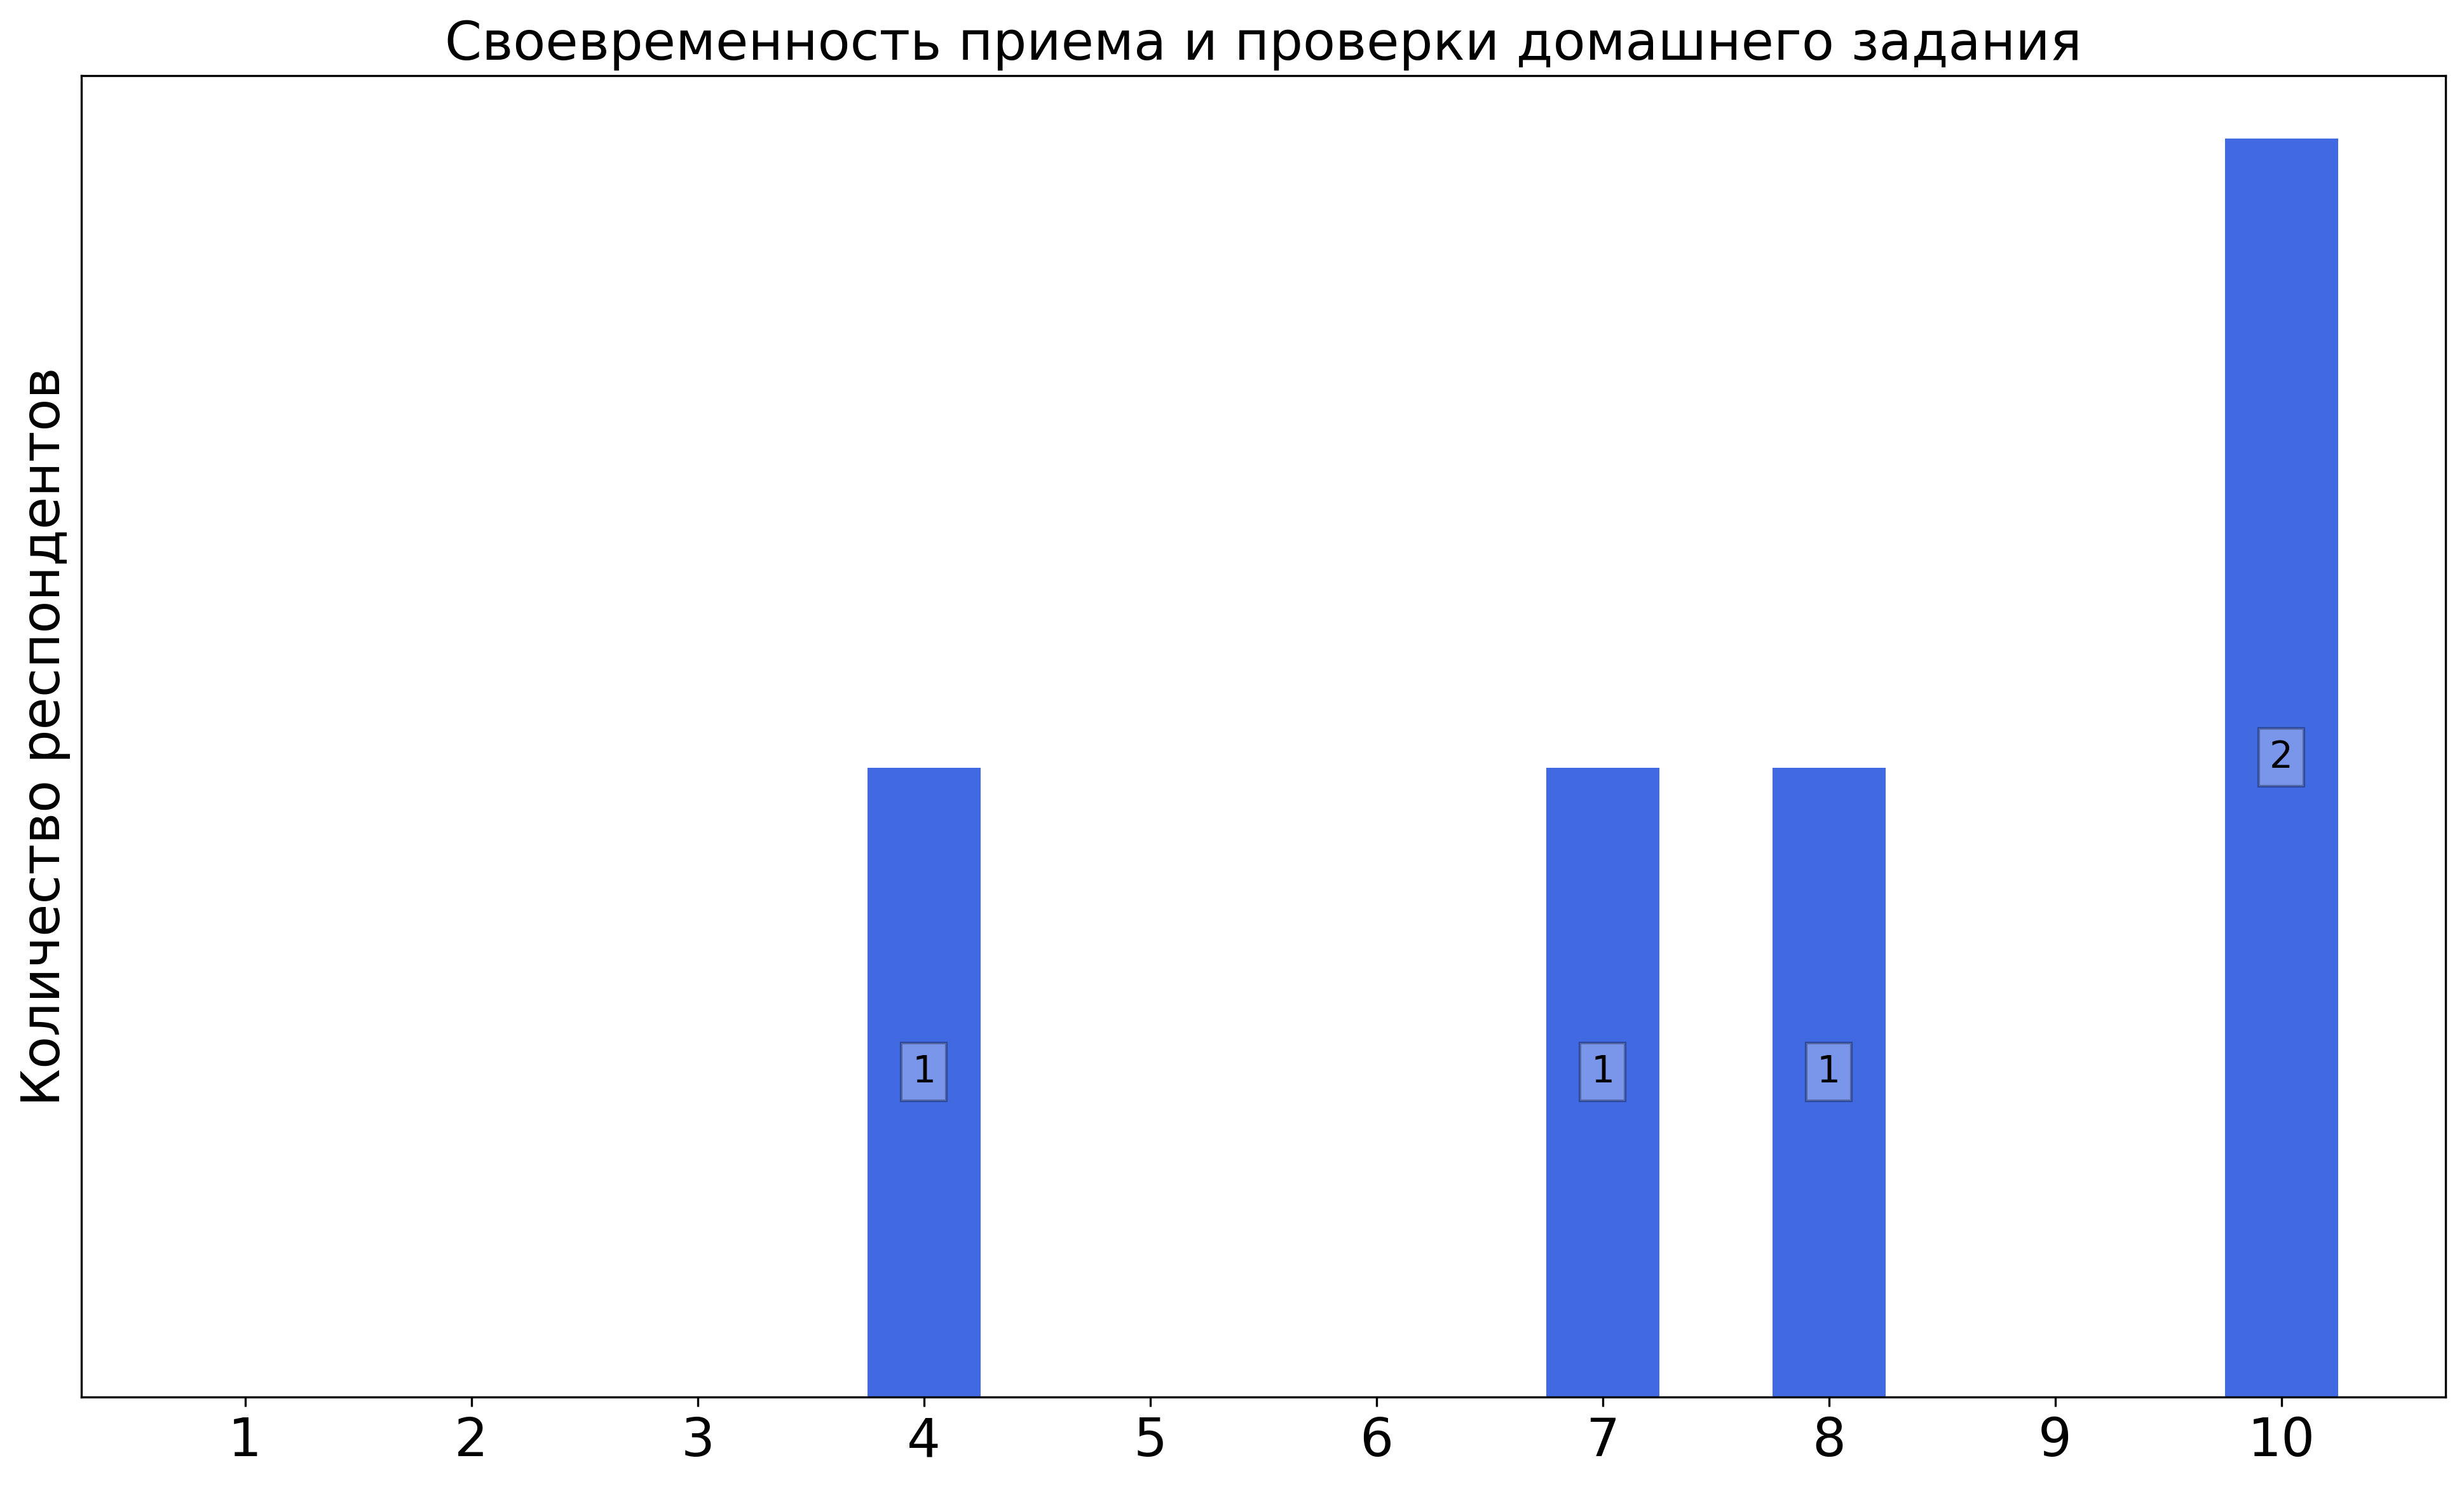
\includegraphics[width=\textwidth]{images/2 course/Общая физика - электричество и магнетизм/seminarists-marks-Седельников Е.В.-2.png}
			\end{subfigure}
			\begin{subfigure}[b]{0.45\textwidth}
				\centering
				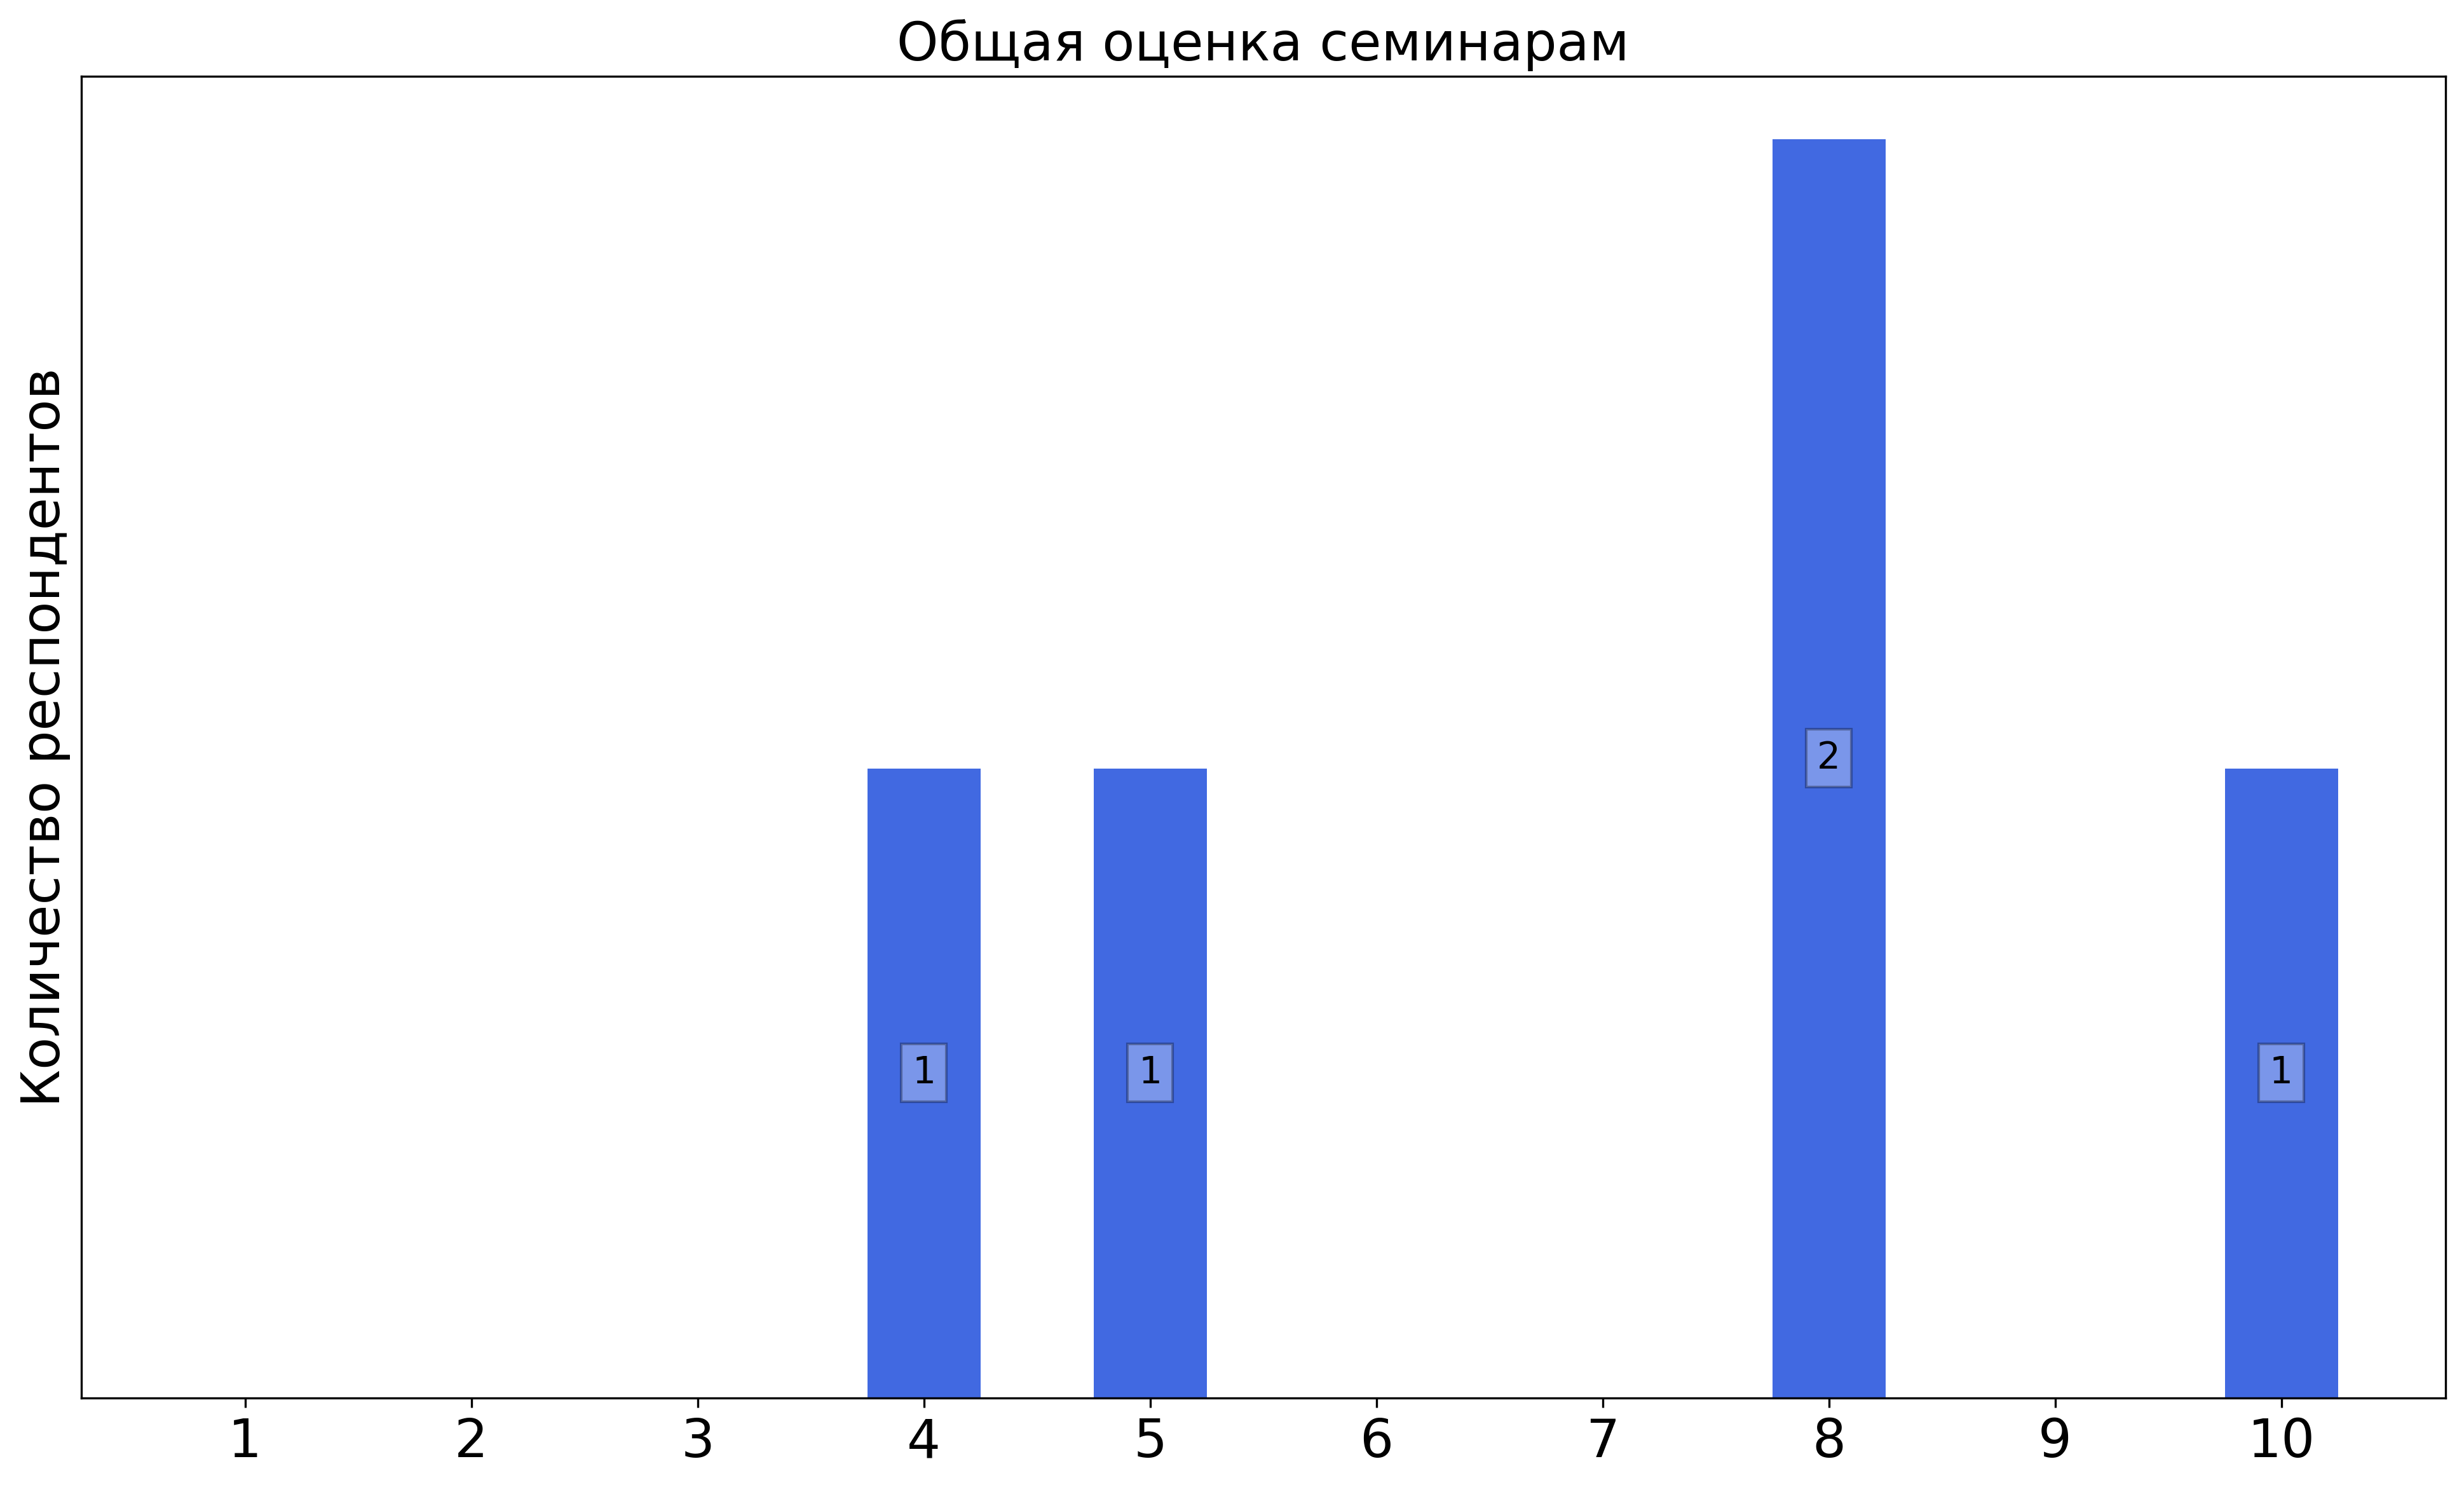
\includegraphics[width=\textwidth]{images/2 course/Общая физика - электричество и магнетизм/seminarists-marks-Седельников Е.В.-3.png}
			\end{subfigure}	
			\caption{Оценки респондентов о качестве преподавания семинаров}
		\end{figure}


	\subsubsection{Отзыв студентов о лабораторных работах. Преподаватель: Галишников А.А.}
		\begin{figure}[H]
			\centering
			\begin{subfigure}[b]{0.45\textwidth}
				\centering
				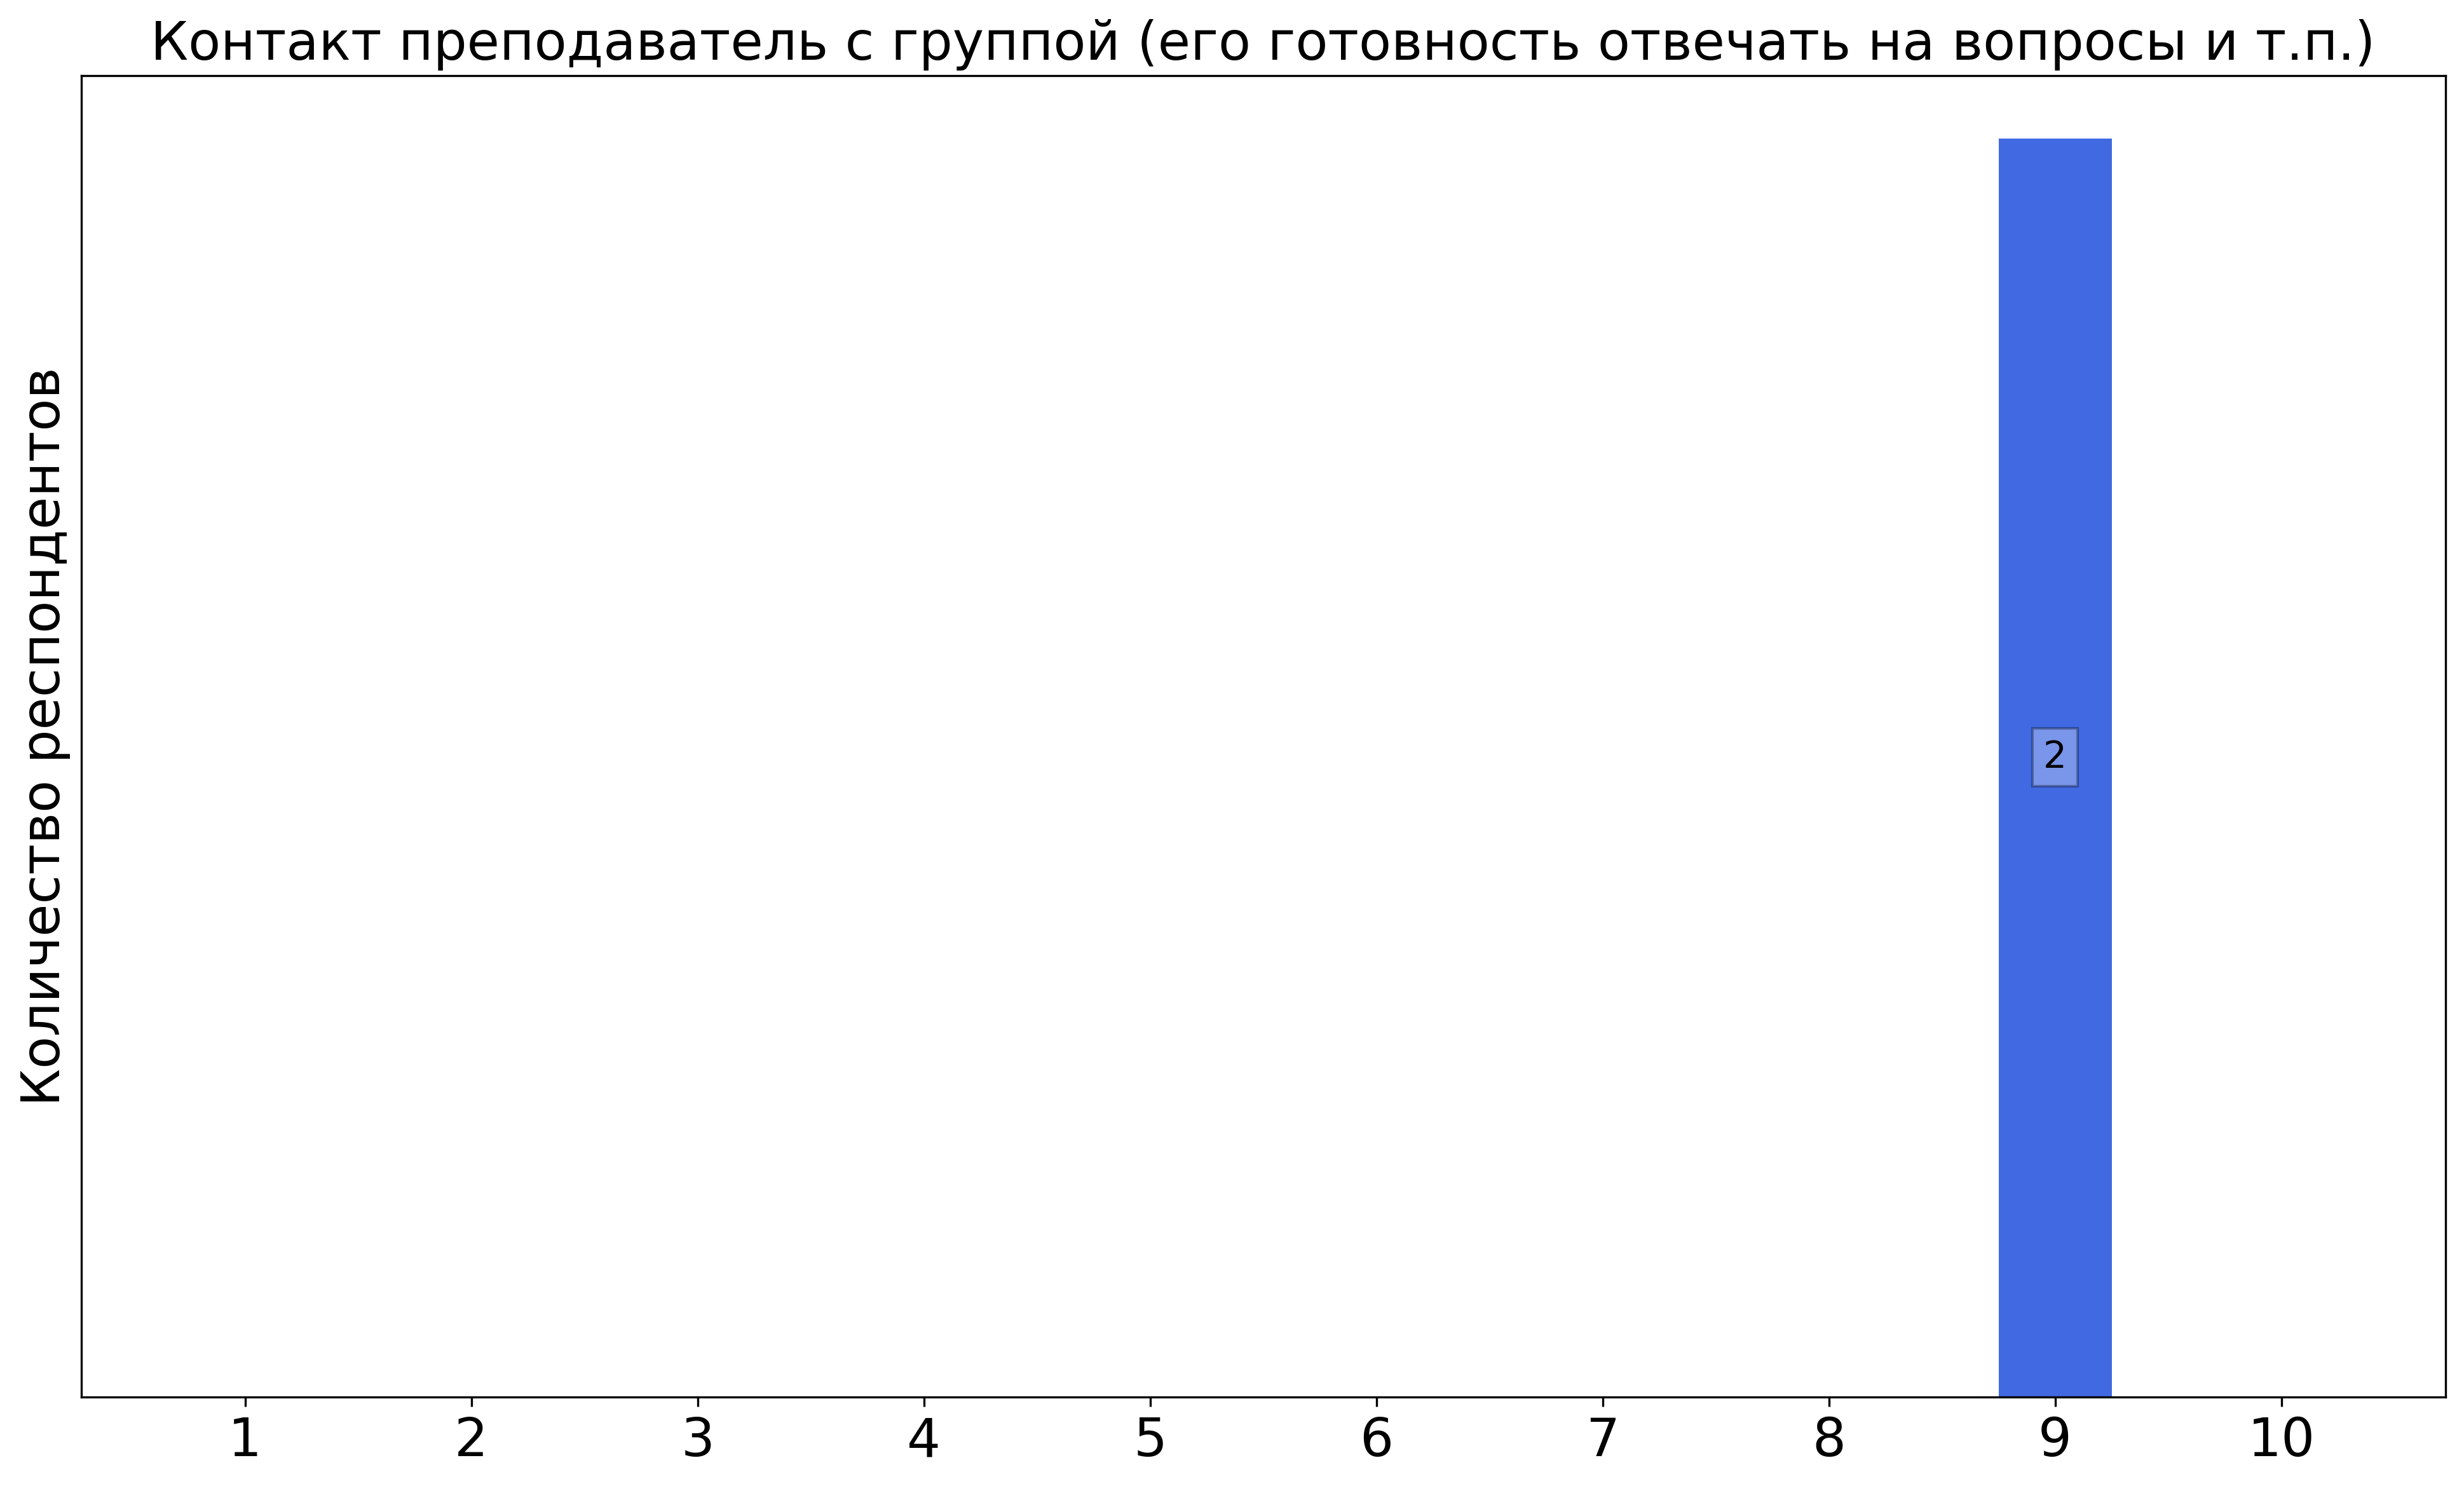
\includegraphics[width=\textwidth]{images/2 course/Общая физика - электричество и магнетизм/labniks-marks-Галишников А.А.-0.png}
			\end{subfigure}
			\begin{subfigure}[b]{0.45\textwidth}
				\centering
				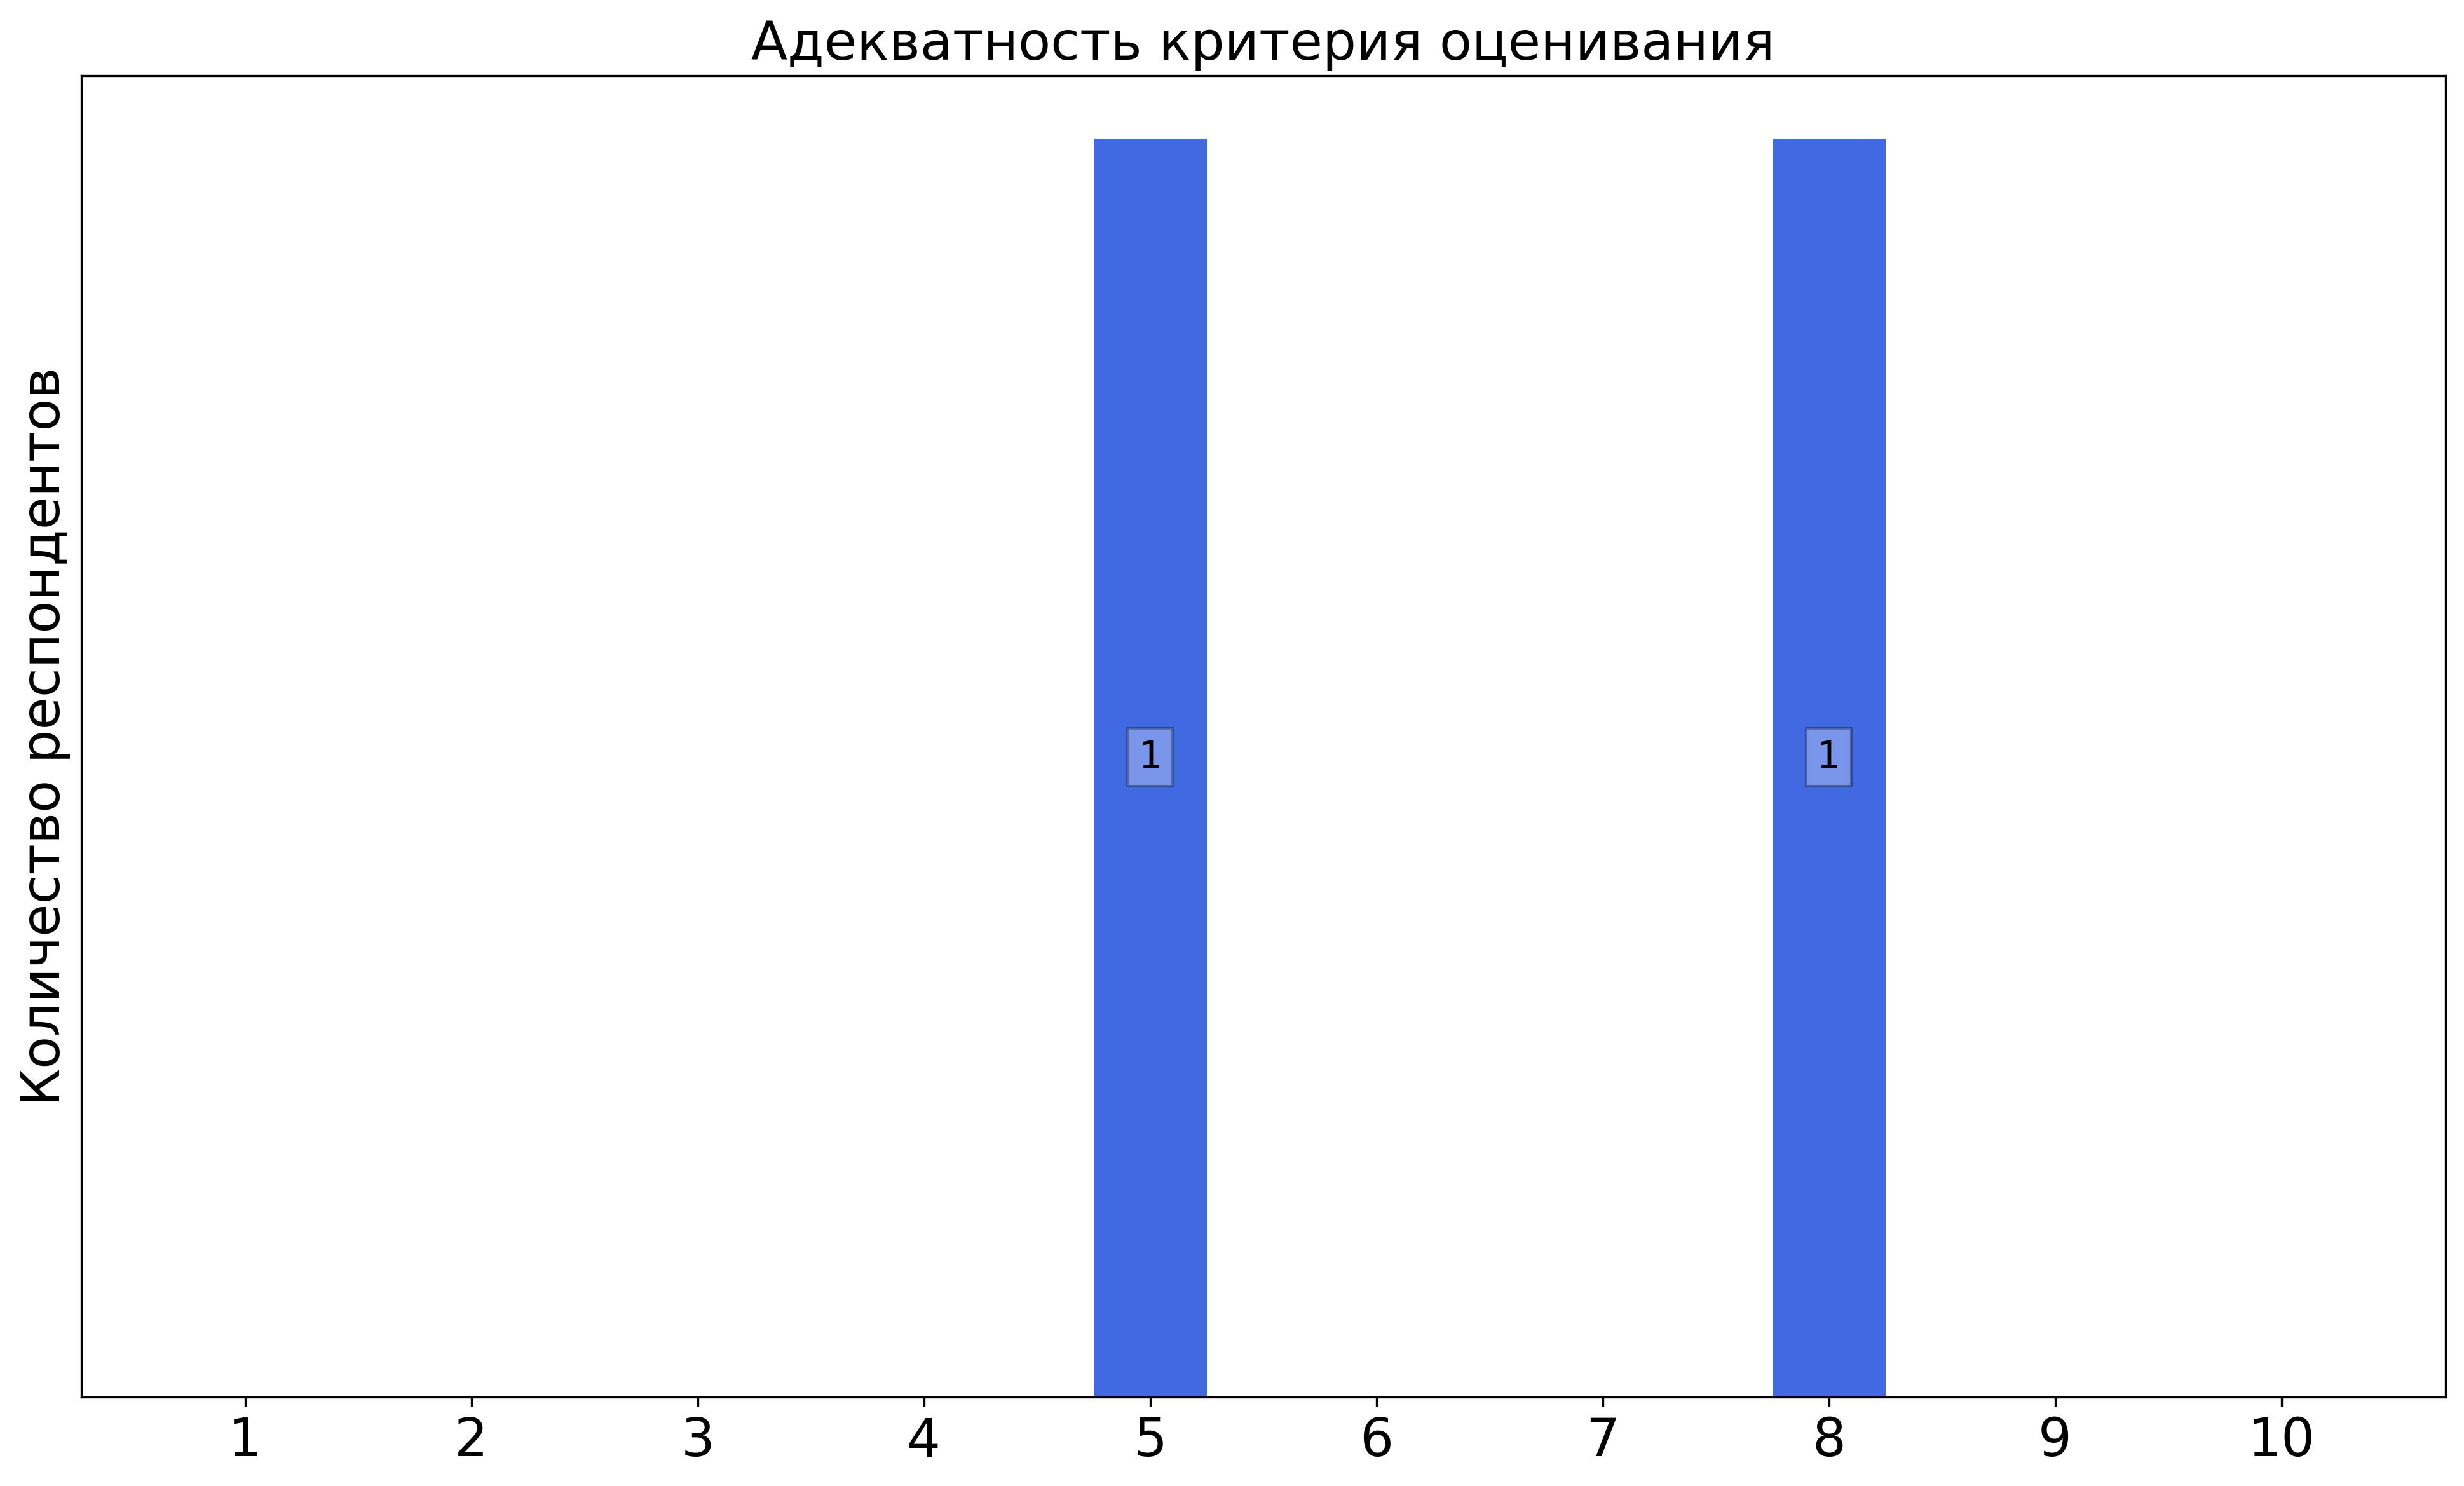
\includegraphics[width=\textwidth]{images/2 course/Общая физика - электричество и магнетизм/labniks-marks-Галишников А.А.-1.png}
			\end{subfigure}
			\begin{subfigure}[b]{0.45\textwidth}
				\centering
				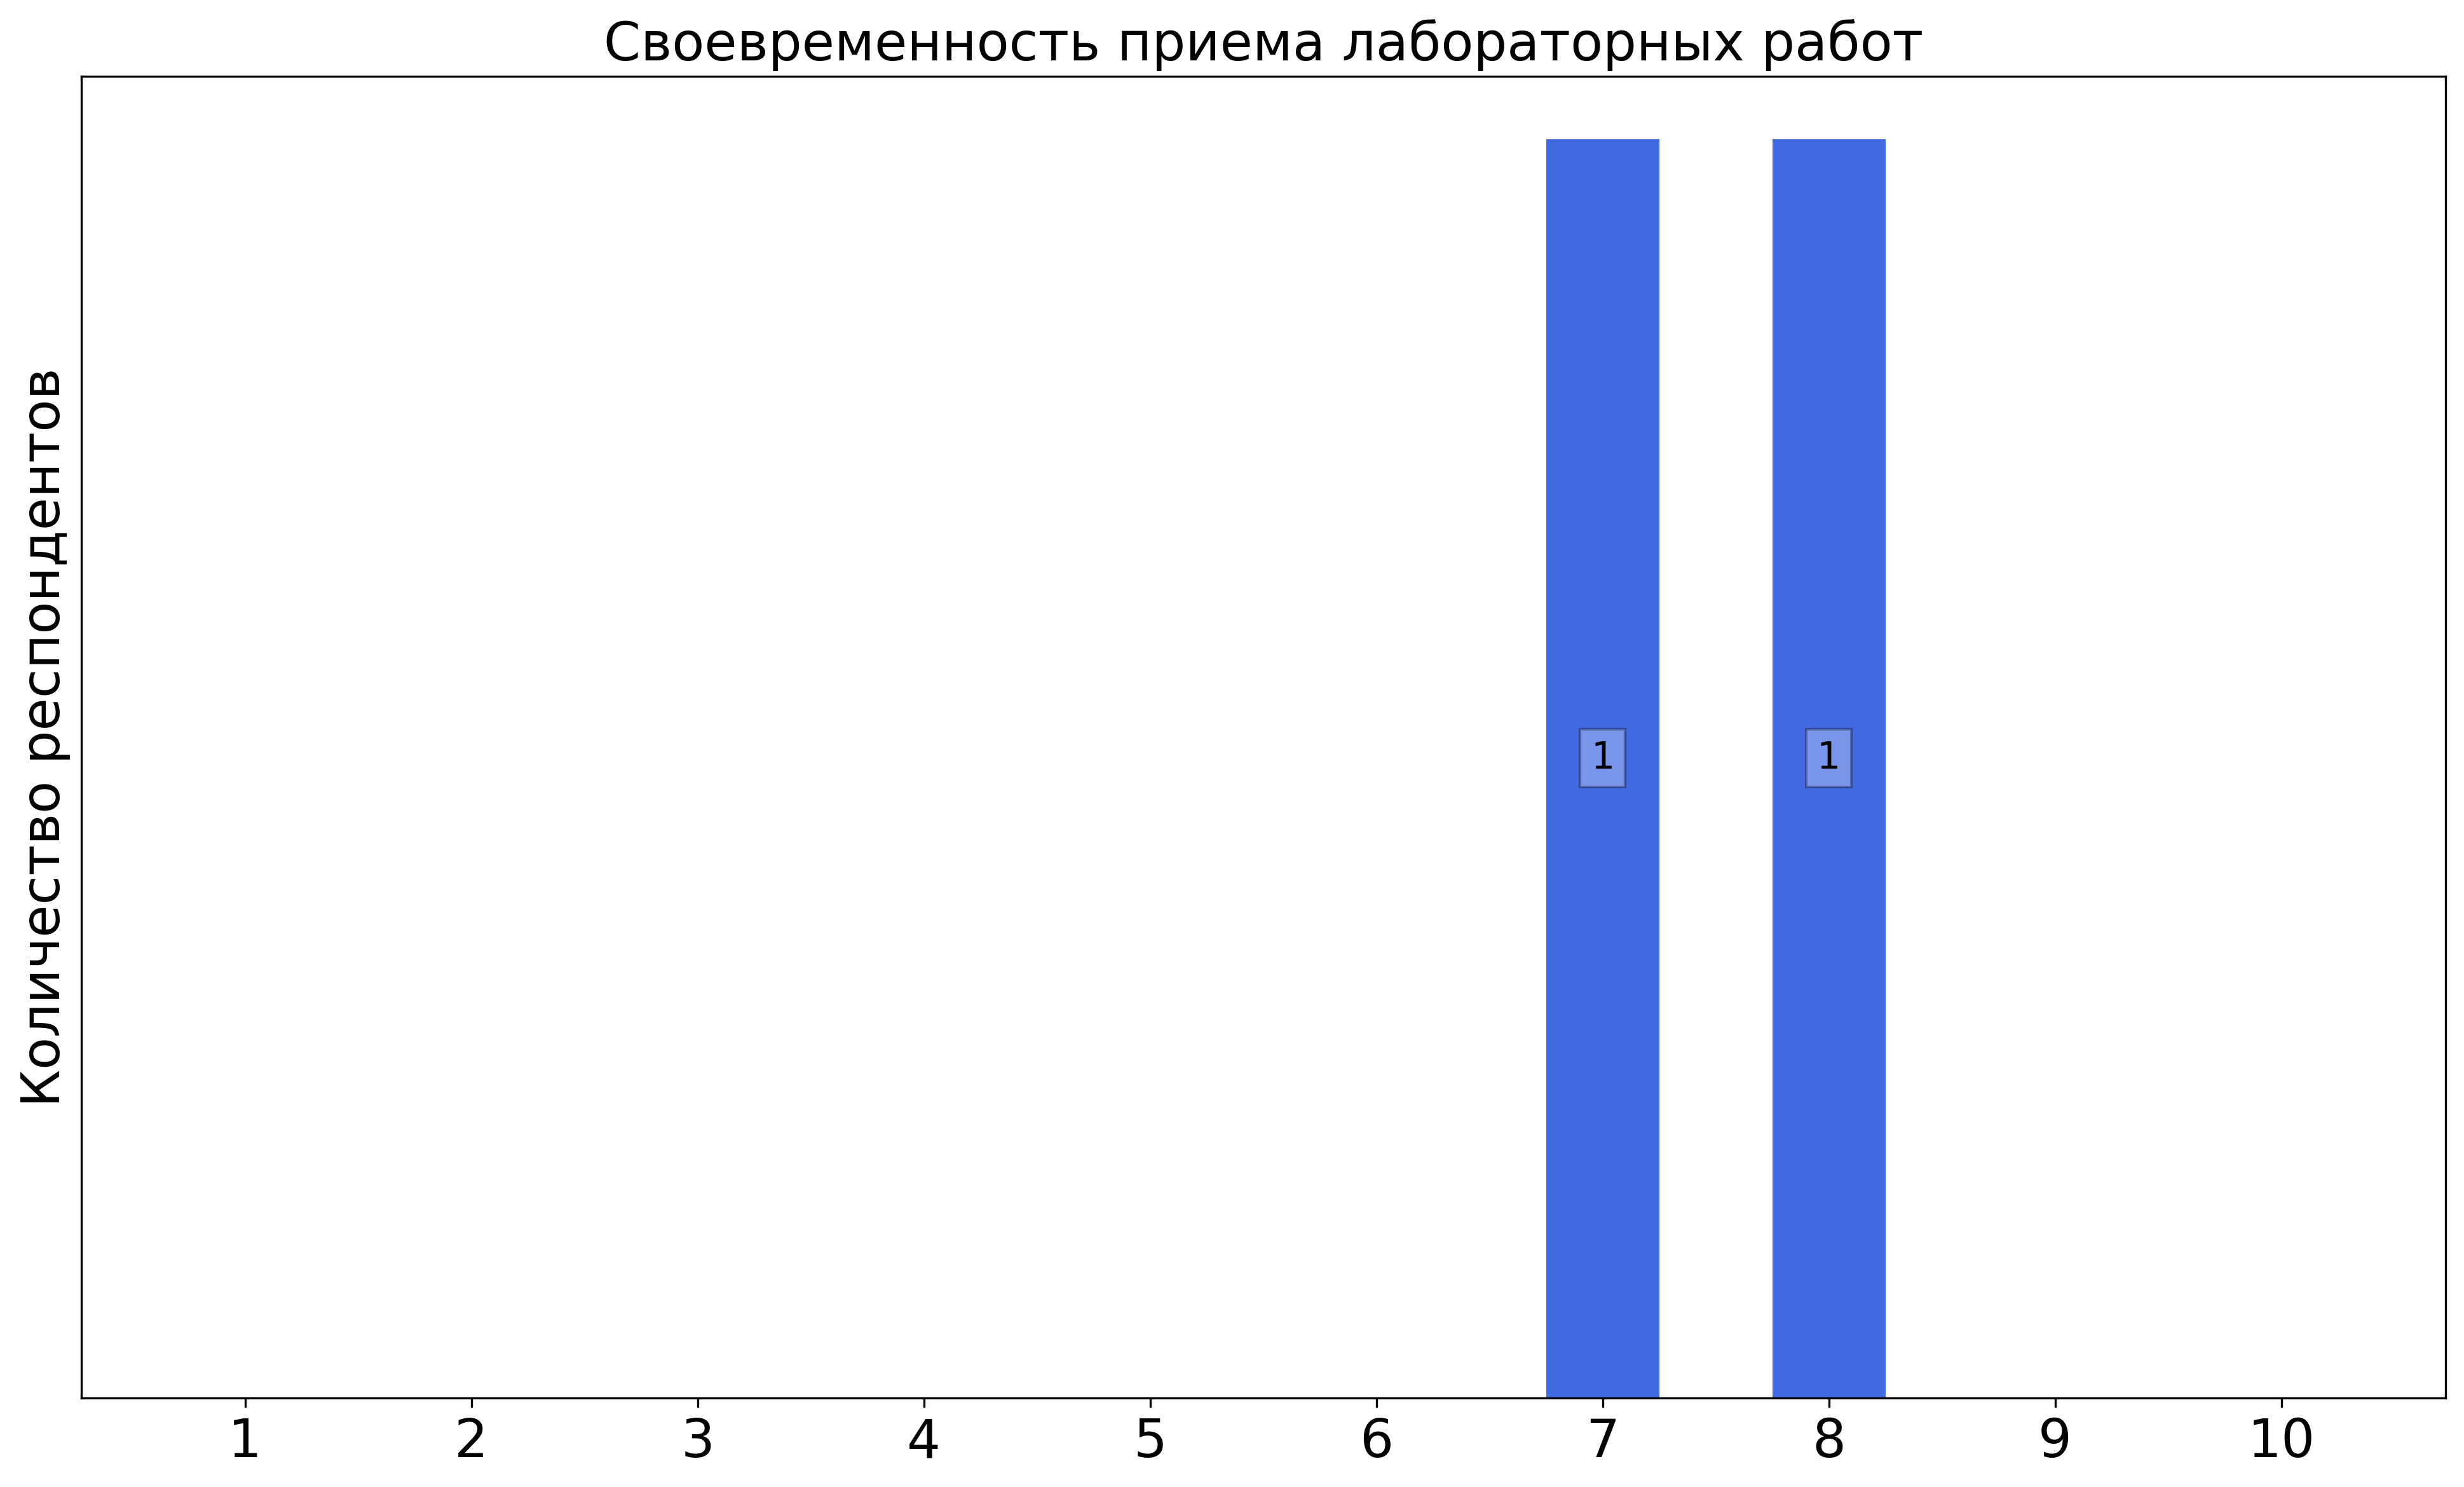
\includegraphics[width=\textwidth]{images/2 course/Общая физика - электричество и магнетизм/labniks-marks-Галишников А.А.-2.png}
			\end{subfigure}
			\begin{subfigure}[b]{0.45\textwidth}
				\centering
				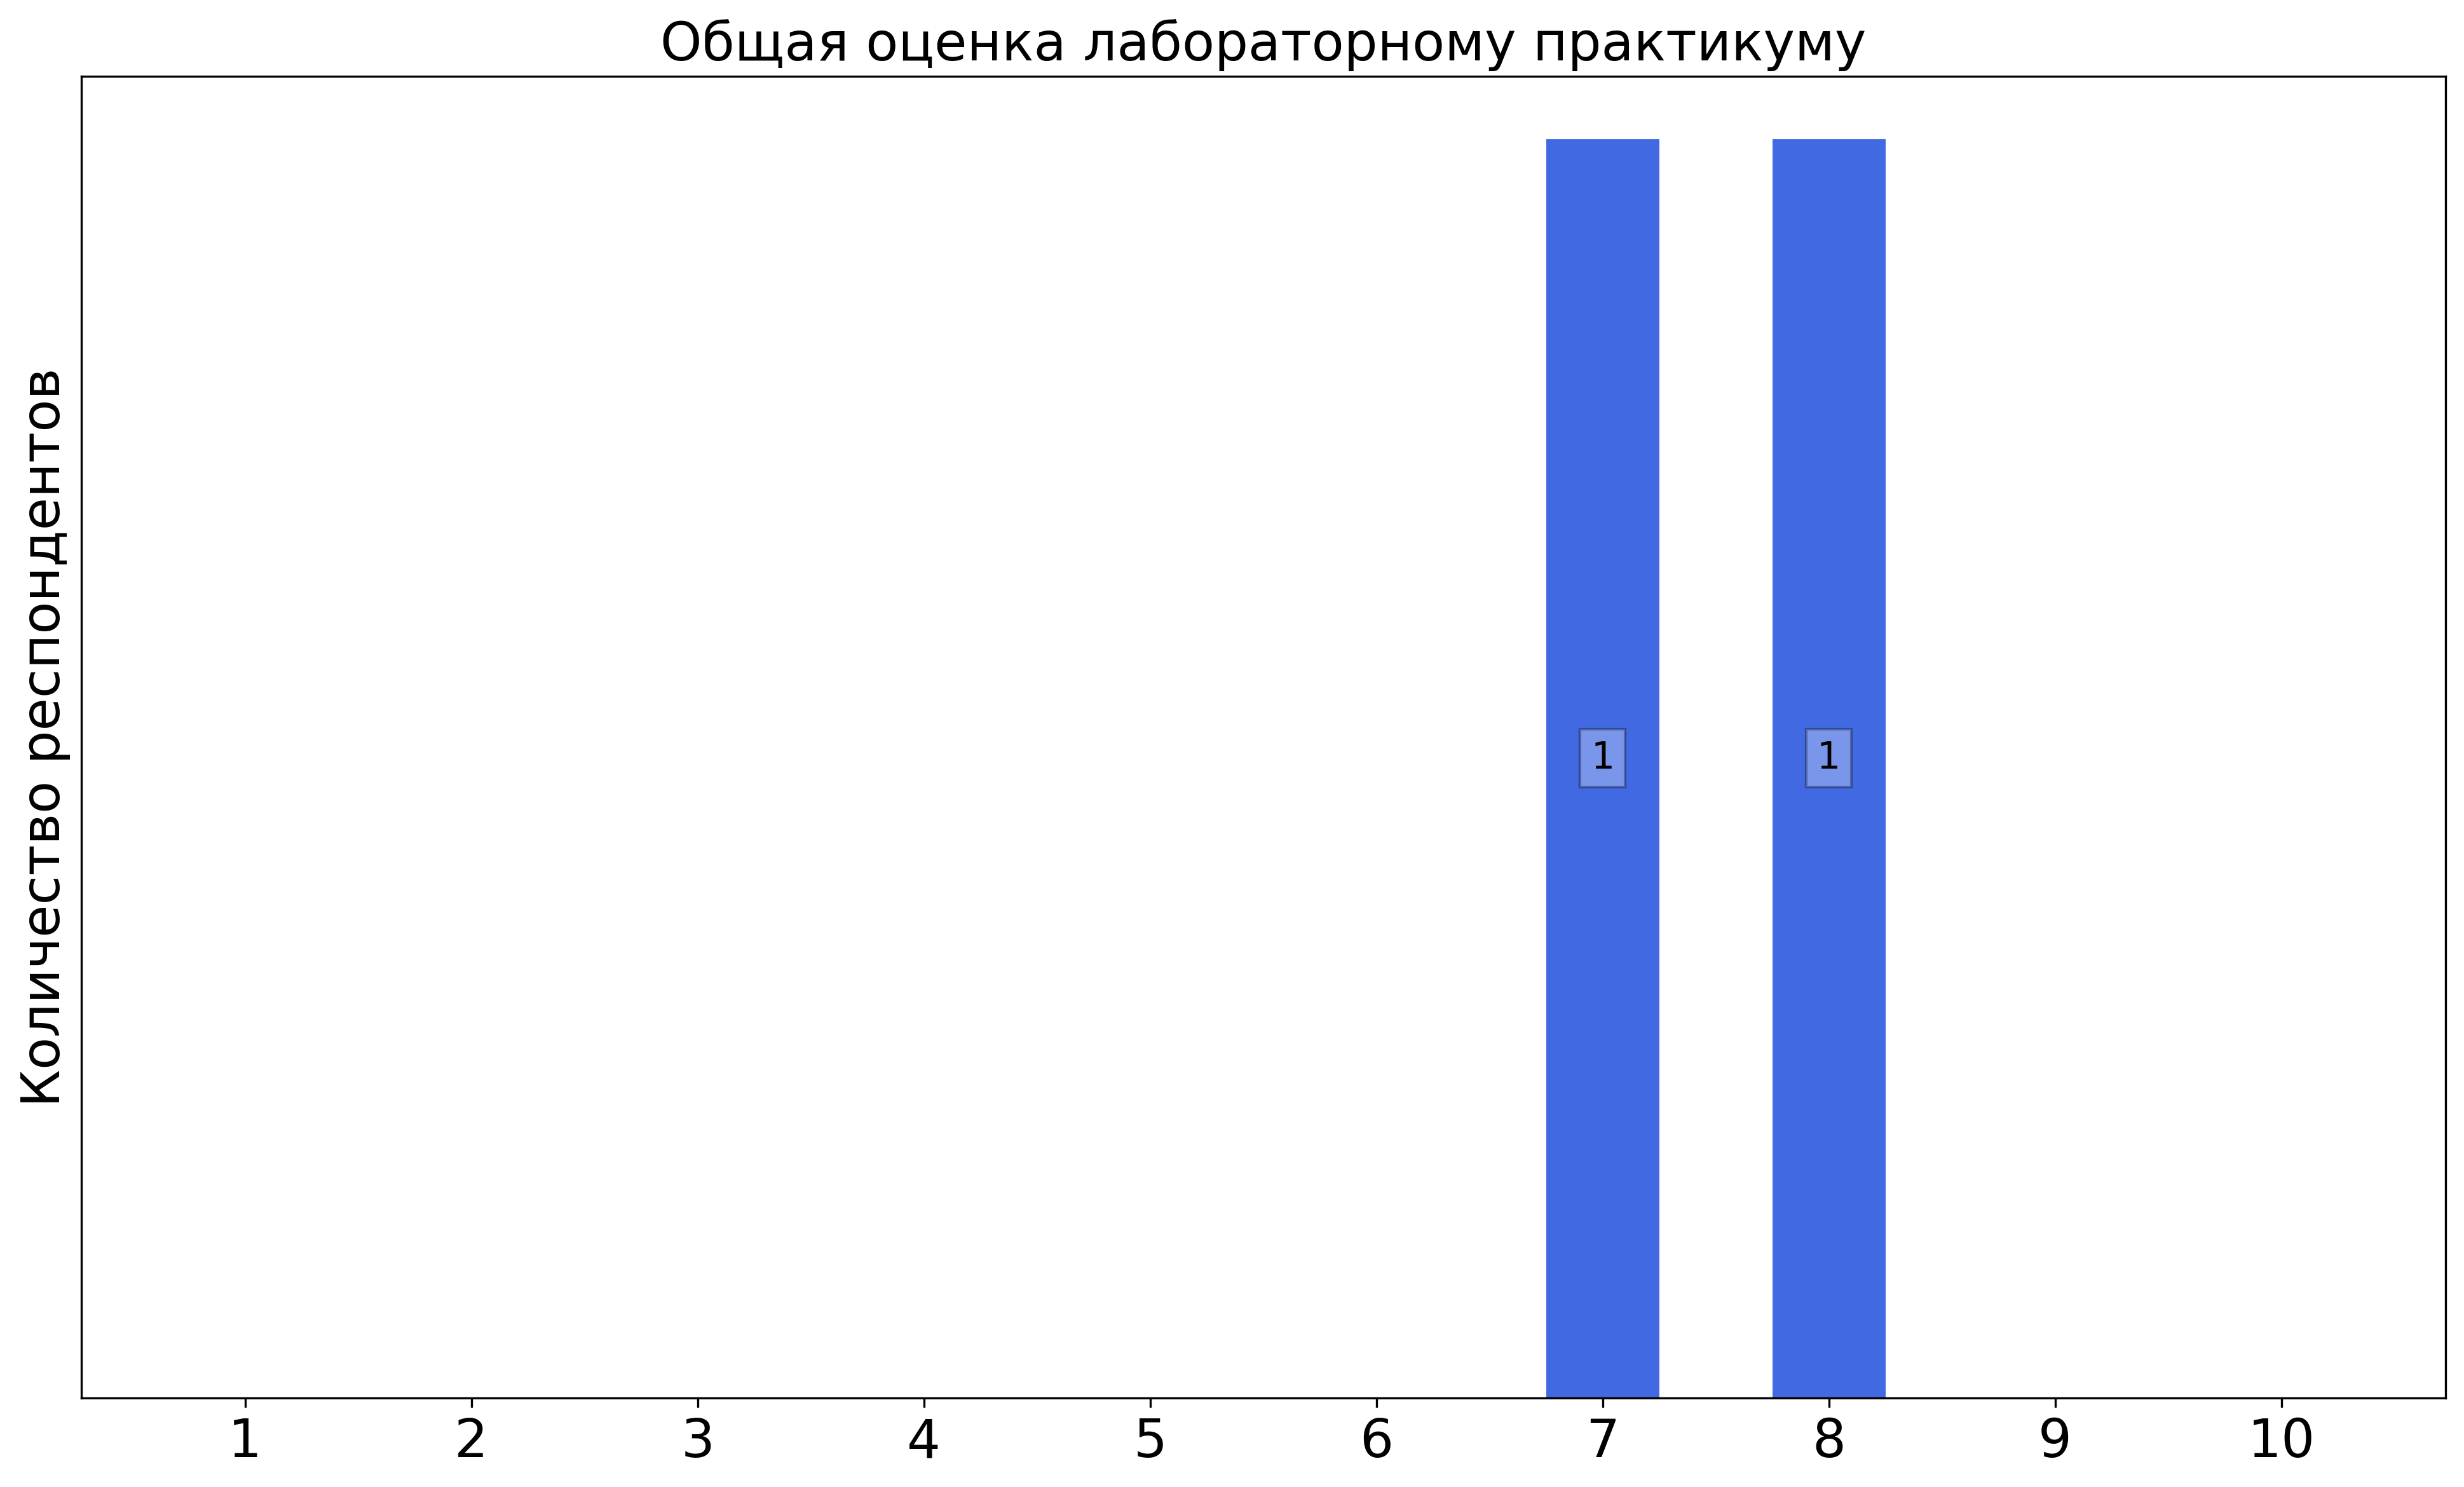
\includegraphics[width=\textwidth]{images/2 course/Общая физика - электричество и магнетизм/labniks-marks-Галишников А.А.-3.png}
			\end{subfigure}	
			\caption{Оценки респондентов о качестве преподавания лабораторных работ}
		\end{figure}


	\subsubsection{Отзыв студентов о лабораторных работах. Преподаватель: Горемыкин И.А.}
		\begin{figure}[H]
			\centering
			\begin{subfigure}[b]{0.45\textwidth}
				\centering
				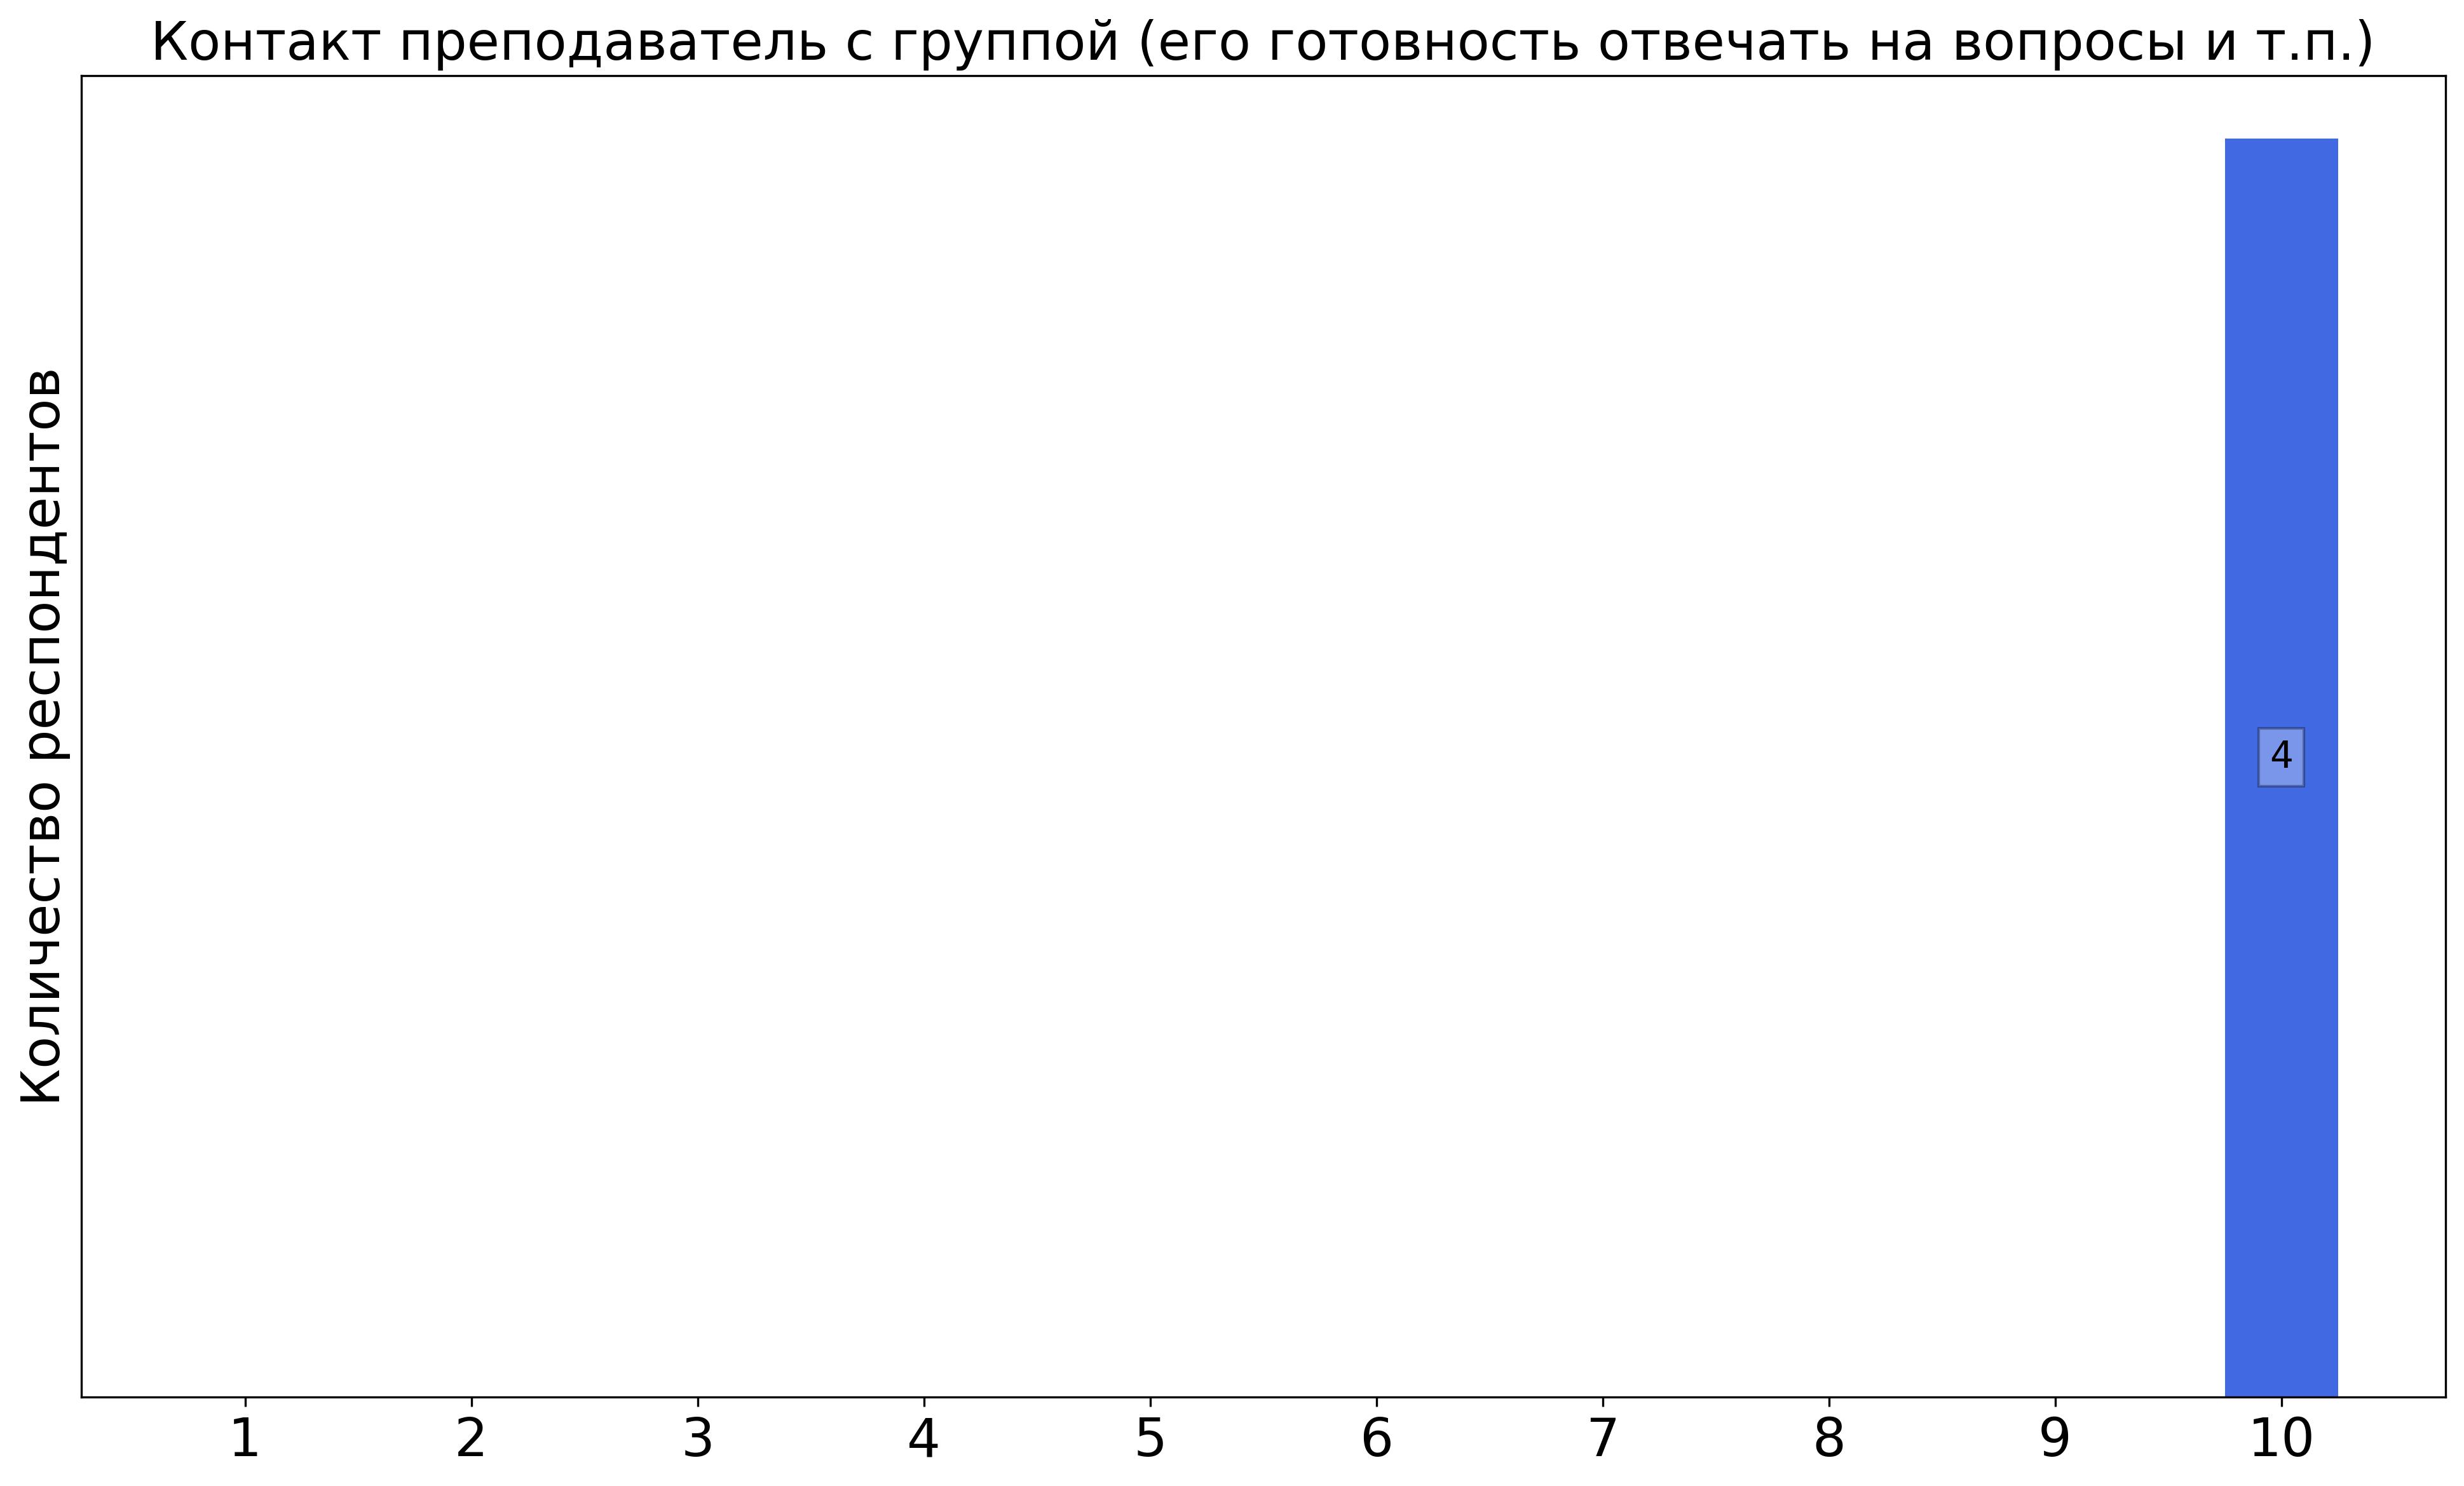
\includegraphics[width=\textwidth]{images/2 course/Общая физика - электричество и магнетизм/labniks-marks-Горемыкин И.А.-0.png}
			\end{subfigure}
			\begin{subfigure}[b]{0.45\textwidth}
				\centering
				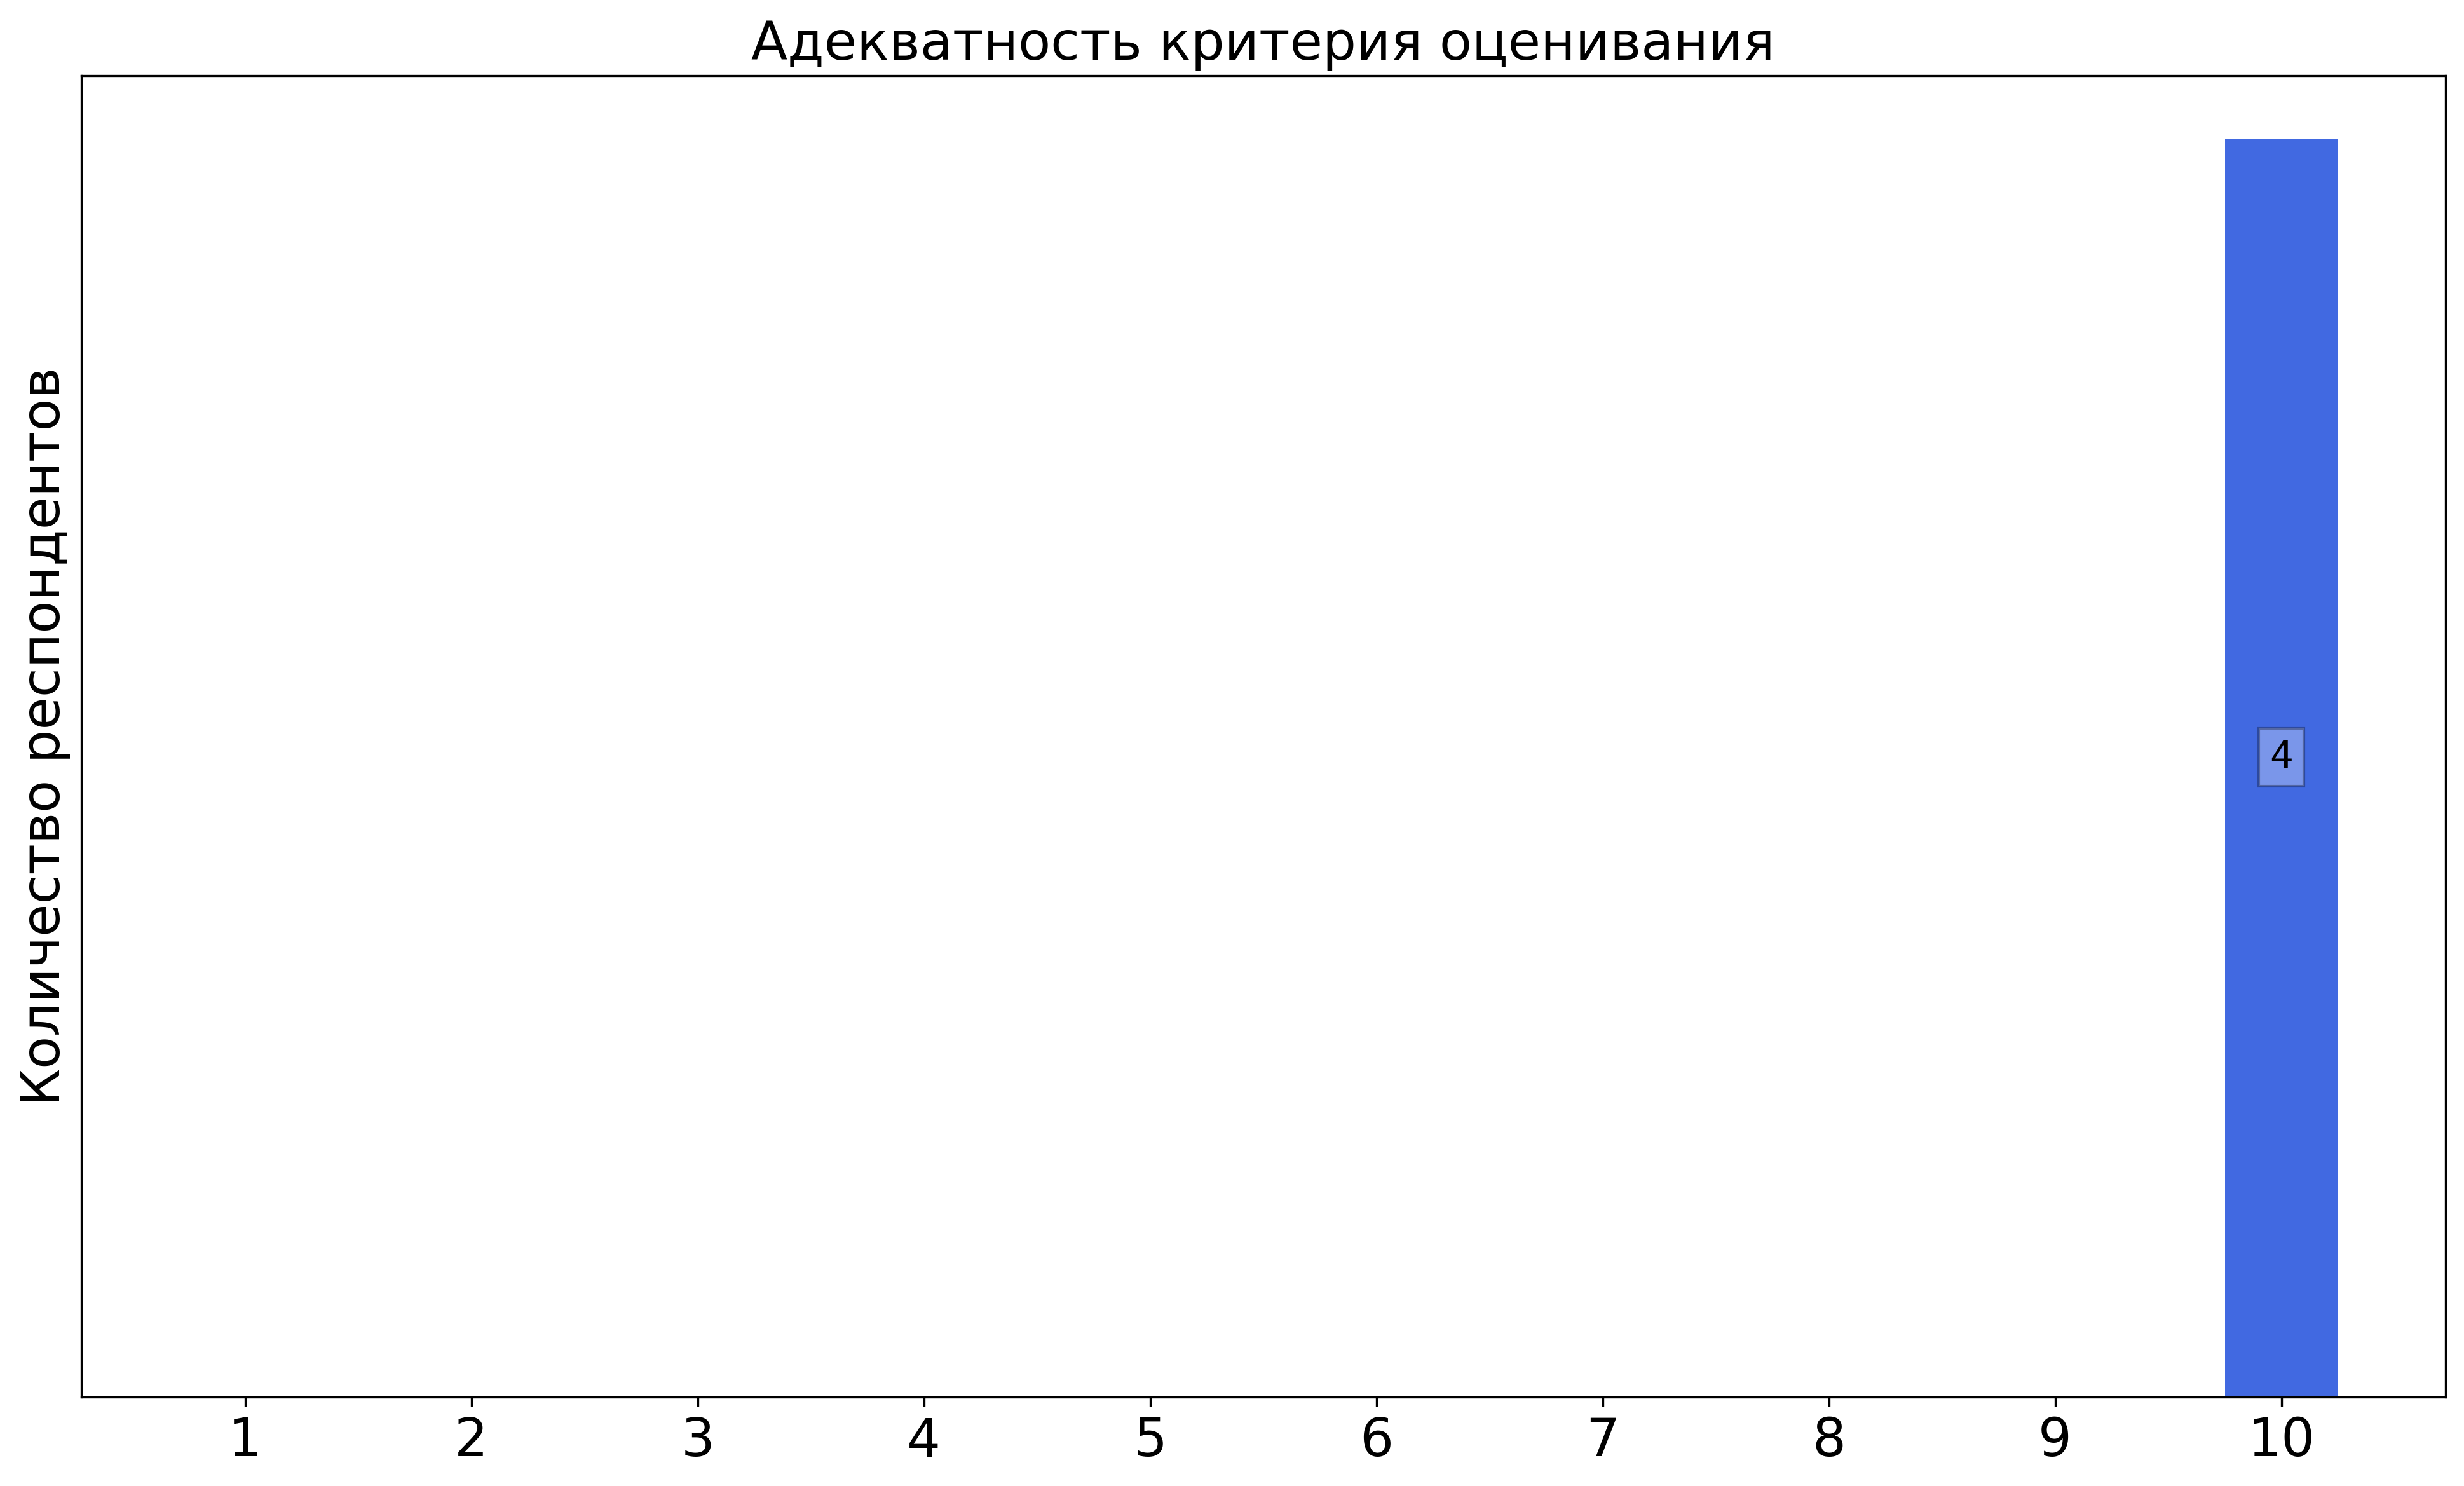
\includegraphics[width=\textwidth]{images/2 course/Общая физика - электричество и магнетизм/labniks-marks-Горемыкин И.А.-1.png}
			\end{subfigure}
			\begin{subfigure}[b]{0.45\textwidth}
				\centering
				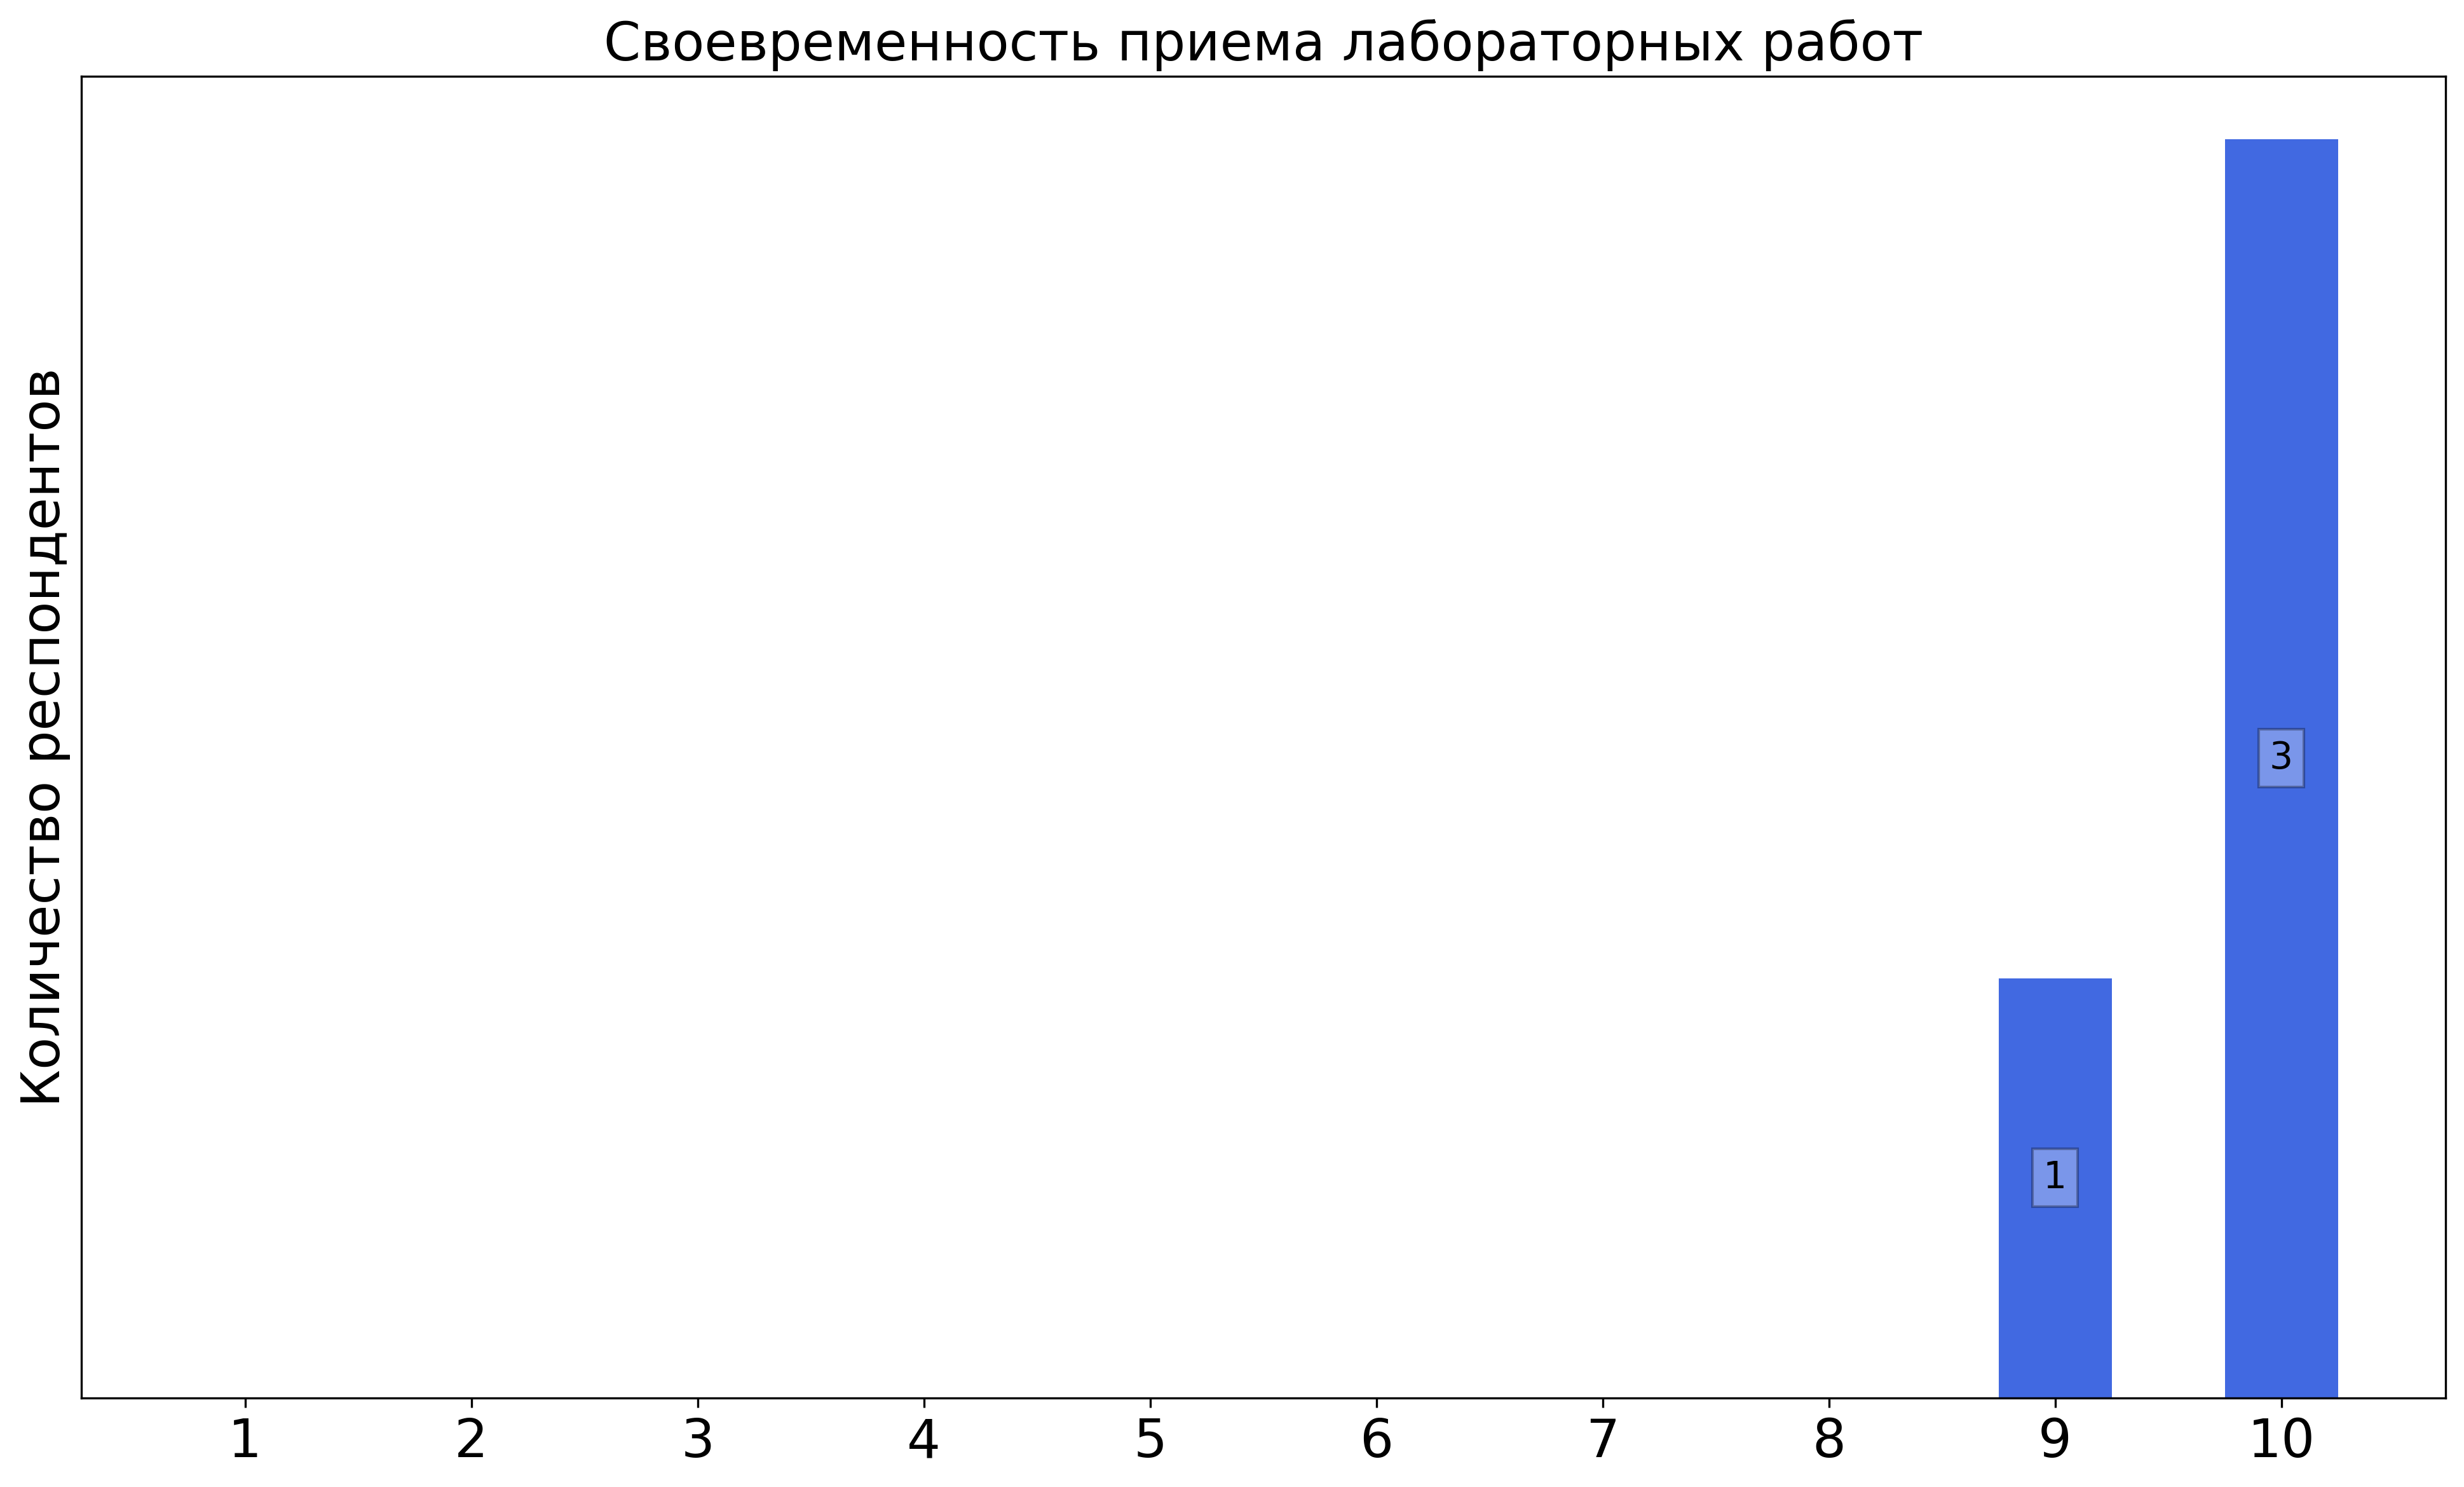
\includegraphics[width=\textwidth]{images/2 course/Общая физика - электричество и магнетизм/labniks-marks-Горемыкин И.А.-2.png}
			\end{subfigure}
			\begin{subfigure}[b]{0.45\textwidth}
				\centering
				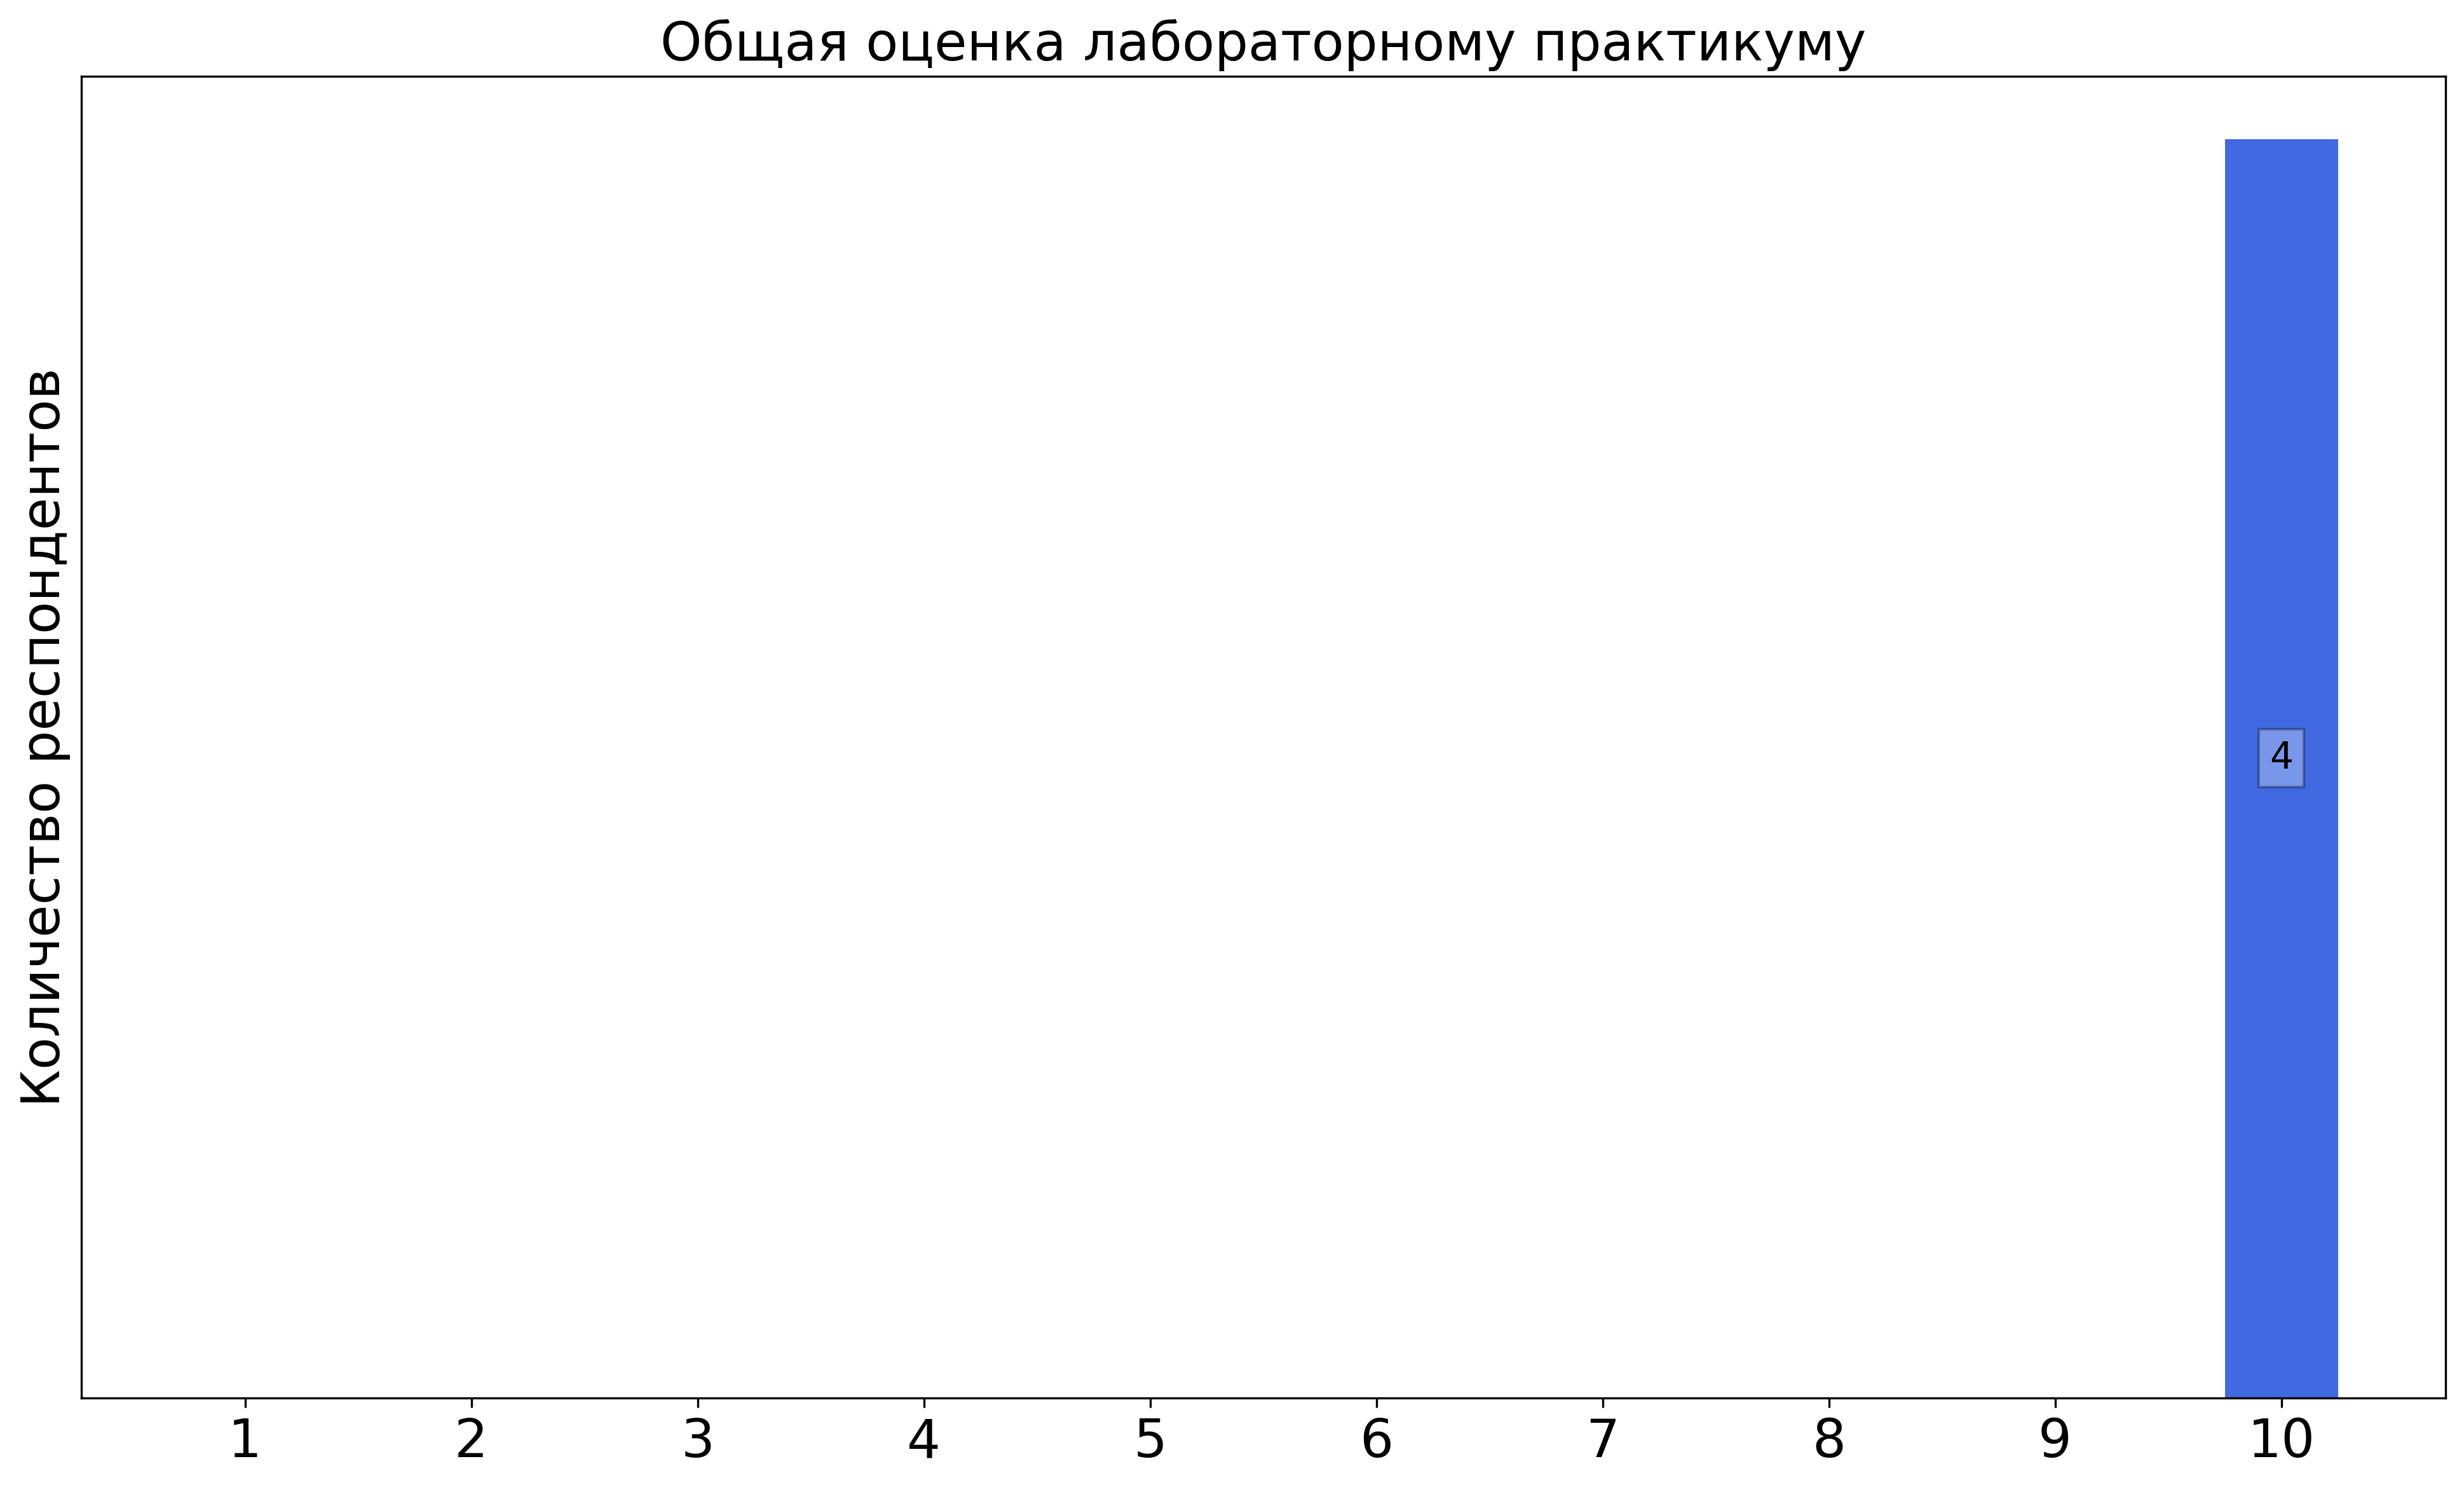
\includegraphics[width=\textwidth]{images/2 course/Общая физика - электричество и магнетизм/labniks-marks-Горемыкин И.А.-3.png}
			\end{subfigure}	
			\caption{Оценки респондентов о качестве преподавания лабораторных работ}
		\end{figure}

	\subsubsection{Отзыв студентов о лабораторных работах. Преподаватель: Джикирба К.Р.}
		\begin{figure}[H]
			\centering
			\begin{subfigure}[b]{0.45\textwidth}
				\centering
				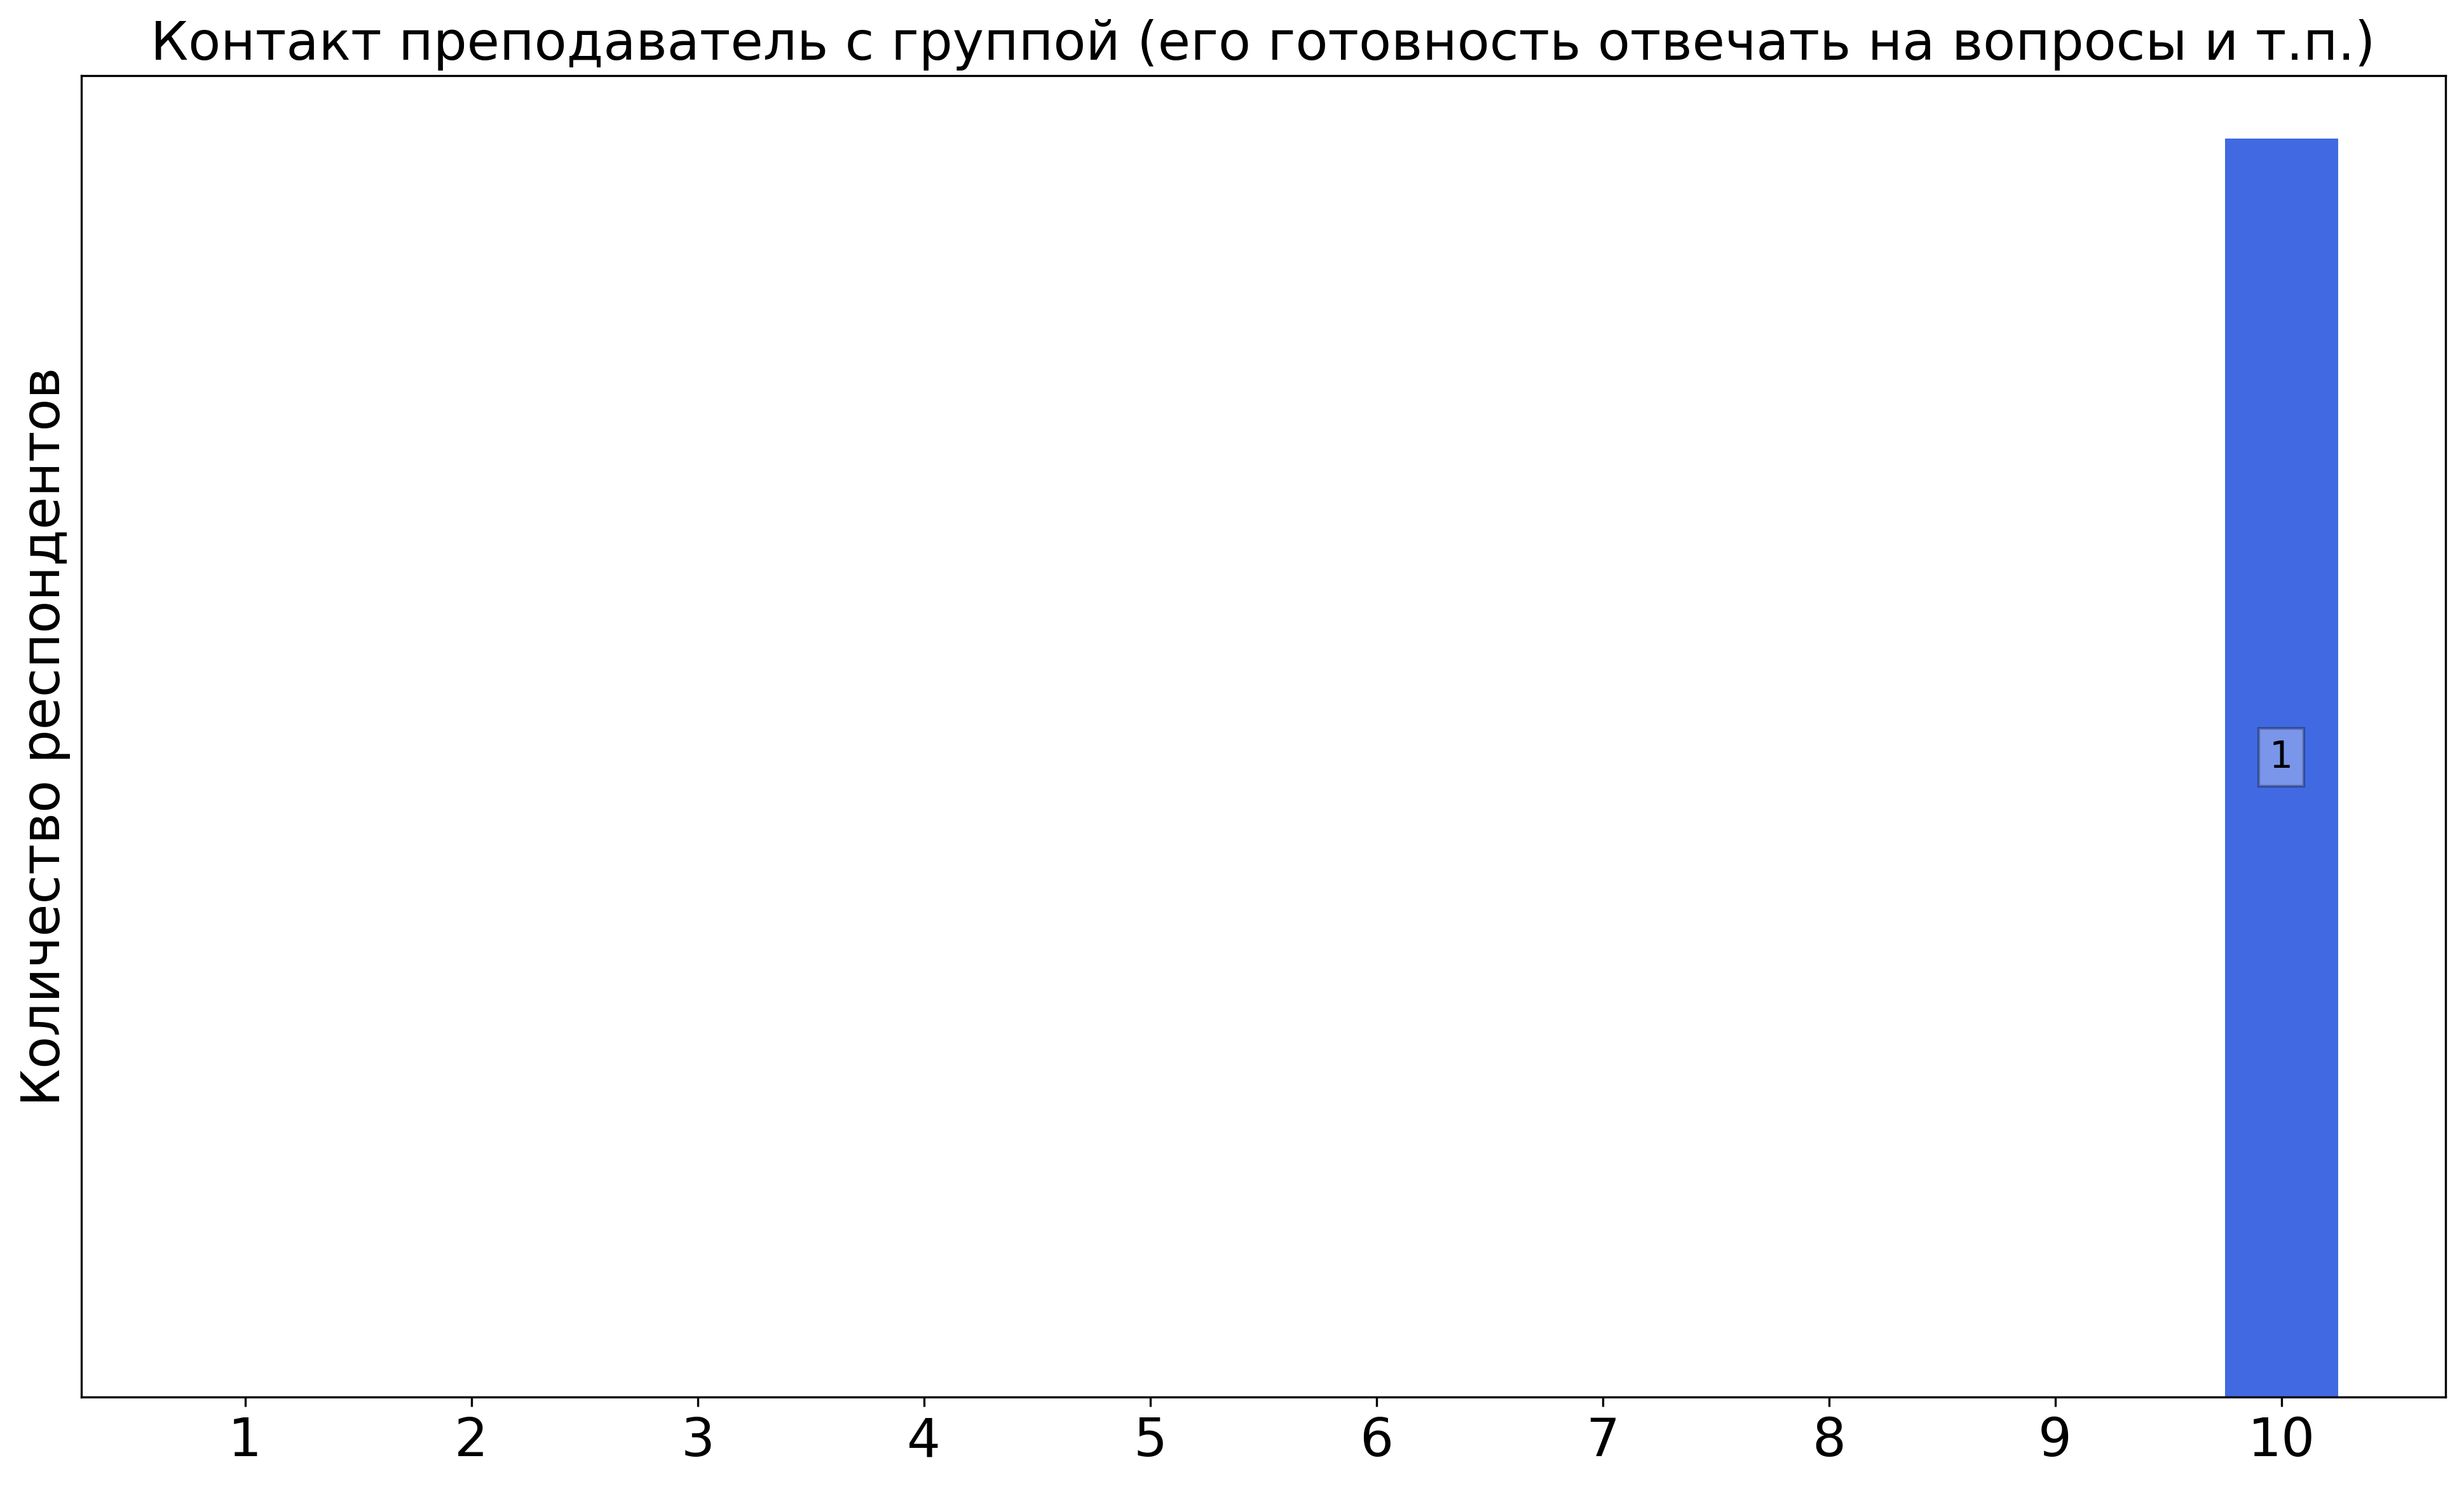
\includegraphics[width=\textwidth]{images/2 course/Общая физика - электричество и магнетизм/labniks-marks-Джикирба К.Р.-0.png}
			\end{subfigure}
			\begin{subfigure}[b]{0.45\textwidth}
				\centering
				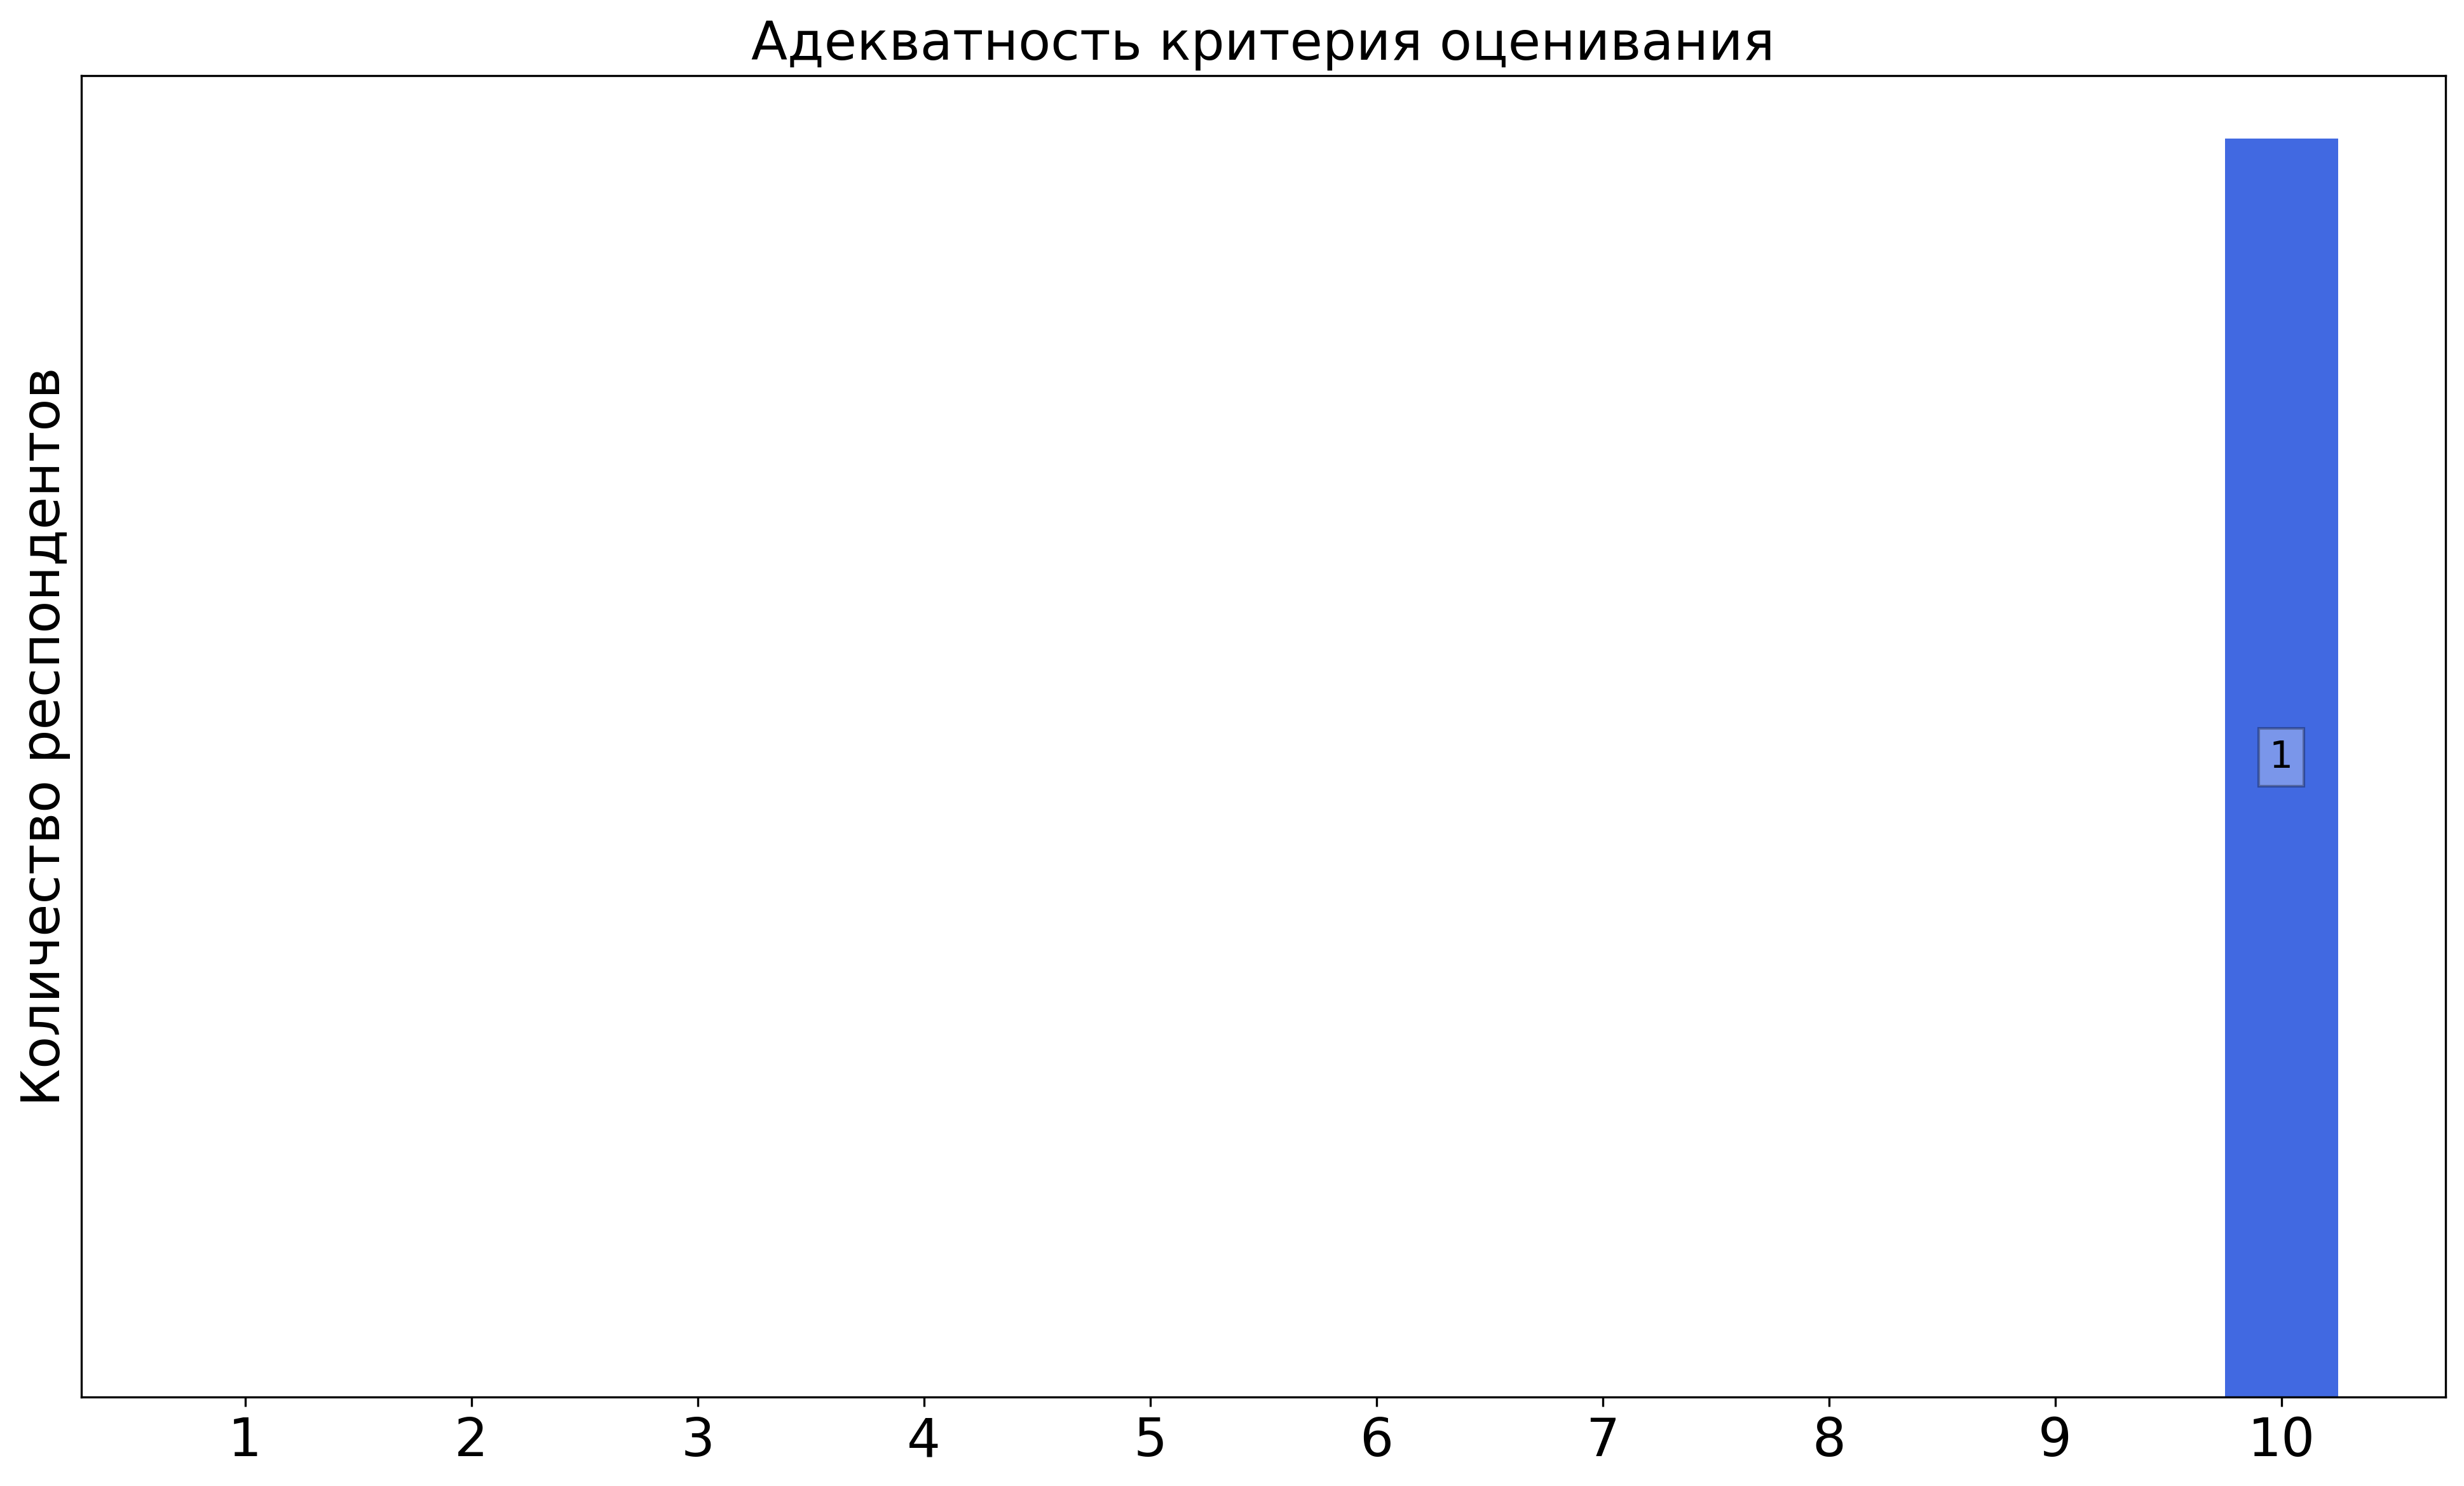
\includegraphics[width=\textwidth]{images/2 course/Общая физика - электричество и магнетизм/labniks-marks-Джикирба К.Р.-1.png}
			\end{subfigure}
			\begin{subfigure}[b]{0.45\textwidth}
				\centering
				\includegraphics[width=\textwidth]{images/2 course/Общая физика - электричество и магнетизм/labniks-marks-Джикирба К.Р.-2.png}
			\end{subfigure}
			\begin{subfigure}[b]{0.45\textwidth}
				\centering
				\includegraphics[width=\textwidth]{images/2 course/Общая физика - электричество и магнетизм/labniks-marks-Джикирба К.Р.-3.png}
			\end{subfigure}	
			\caption{Оценки респондентов о качестве преподавания лабораторных работ}
		\end{figure}


	\subsubsection{Отзыв студентов о лабораторных работах. Преподаватель: Долгих В.А.}
		\begin{figure}[H]
			\centering
			\begin{subfigure}[b]{0.45\textwidth}
				\centering
				\includegraphics[width=\textwidth]{images/2 course/Общая физика - электричество и магнетизм/labniks-marks-Долгих В.А.-0.png}
			\end{subfigure}
			\begin{subfigure}[b]{0.45\textwidth}
				\centering
				\includegraphics[width=\textwidth]{images/2 course/Общая физика - электричество и магнетизм/labniks-marks-Долгих В.А.-1.png}
			\end{subfigure}
			\begin{subfigure}[b]{0.45\textwidth}
				\centering
				\includegraphics[width=\textwidth]{images/2 course/Общая физика - электричество и магнетизм/labniks-marks-Долгих В.А.-2.png}
			\end{subfigure}
			\begin{subfigure}[b]{0.45\textwidth}
				\centering
				\includegraphics[width=\textwidth]{images/2 course/Общая физика - электричество и магнетизм/labniks-marks-Долгих В.А.-3.png}
			\end{subfigure}	
			\caption{Оценки респондентов о качестве преподавания лабораторных работ}
		\end{figure}

		\textbf{Комментарии студентов о преподавателе\protect\footnote{сохранены оригинальные орфография и пунктуация}}

		\begin{commentbox} 
			Свое понимание физики которое я не понимаю 
		\end{commentbox} 
	   
		\begin{commentbox} 
			Очень жестко принимал лабы, непонятны критерии оценивания и какой именно ответ он от тебя требует. 
		\end{commentbox} 

    
	\subsubsection{Отзыв студентов о лабораторных работах. Преподаватель: Максимычев А.В.}
		\begin{figure}[H]
			\centering
			\begin{subfigure}[b]{0.45\textwidth}
				\centering
				\includegraphics[width=\textwidth]{images/2 course/Общая физика - электричество и магнетизм/labniks-marks-Максимычев А.В.-0.png}
			\end{subfigure}
			\begin{subfigure}[b]{0.45\textwidth}
				\centering
				\includegraphics[width=\textwidth]{images/2 course/Общая физика - электричество и магнетизм/labniks-marks-Максимычев А.В.-1.png}
			\end{subfigure}
			\begin{subfigure}[b]{0.45\textwidth}
				\centering
				\includegraphics[width=\textwidth]{images/2 course/Общая физика - электричество и магнетизм/labniks-marks-Максимычев А.В.-2.png}
			\end{subfigure}
			\begin{subfigure}[b]{0.45\textwidth}
				\centering
				\includegraphics[width=\textwidth]{images/2 course/Общая физика - электричество и магнетизм/labniks-marks-Максимычев А.В.-3.png}
			\end{subfigure}	
			\caption{Оценки респондентов о качестве преподавания лабораторных работ}
		\end{figure}

		\textbf{Комментарии студентов о преподавателе\protect\footnote{сохранены оригинальные орфография и пунктуация}}


	\subsubsection{Отзыв студентов о лабораторных работах. Преподаватель: Меньших Н.Л.}
		\begin{figure}[H]
			\centering
			\begin{subfigure}[b]{0.45\textwidth}
				\centering
				\includegraphics[width=\textwidth]{images/2 course/Общая физика - электричество и магнетизм/labniks-marks-Меньших Н.Л.-0.png}
			\end{subfigure}
			\begin{subfigure}[b]{0.45\textwidth}
				\centering
				\includegraphics[width=\textwidth]{images/2 course/Общая физика - электричество и магнетизм/labniks-marks-Меньших Н.Л.-1.png}
			\end{subfigure}
			\begin{subfigure}[b]{0.45\textwidth}
				\centering
				\includegraphics[width=\textwidth]{images/2 course/Общая физика - электричество и магнетизм/labniks-marks-Меньших Н.Л.-2.png}
			\end{subfigure}
			\begin{subfigure}[b]{0.45\textwidth}
				\centering
				\includegraphics[width=\textwidth]{images/2 course/Общая физика - электричество и магнетизм/labniks-marks-Меньших Н.Л.-3.png}
			\end{subfigure}	
			\caption{Оценки респондентов о качестве преподавания лабораторных работ}
		\end{figure}


	\subsubsection{Отзыв студентов о лабораторных работах. Преподаватель: Нухов А.К.}
		\begin{figure}[H]
			\centering
			\begin{subfigure}[b]{0.45\textwidth}
				\centering
				\includegraphics[width=\textwidth]{images/2 course/Общая физика - электричество и магнетизм/labniks-marks-Нухов А.К.-0.png}
			\end{subfigure}
			\begin{subfigure}[b]{0.45\textwidth}
				\centering
				\includegraphics[width=\textwidth]{images/2 course/Общая физика - электричество и магнетизм/labniks-marks-Нухов А.К.-1.png}
			\end{subfigure}
			\begin{subfigure}[b]{0.45\textwidth}
				\centering
				\includegraphics[width=\textwidth]{images/2 course/Общая физика - электричество и магнетизм/labniks-marks-Нухов А.К.-2.png}
			\end{subfigure}
			\begin{subfigure}[b]{0.45\textwidth}
				\centering
				\includegraphics[width=\textwidth]{images/2 course/Общая физика - электричество и магнетизм/labniks-marks-Нухов А.К.-3.png}
			\end{subfigure}	
			\caption{Оценки респондентов о качестве преподавания лабораторных работ}
		\end{figure}


	\subsubsection{Отзыв студентов о лабораторных работах. Преподаватель: Пауков М.И.}
		\begin{figure}[H]
			\centering
			\begin{subfigure}[b]{0.45\textwidth}
				\centering
				\includegraphics[width=\textwidth]{images/2 course/Общая физика - электричество и магнетизм/labniks-marks-Пауков М.И.-0.png}
			\end{subfigure}
			\begin{subfigure}[b]{0.45\textwidth}
				\centering
				\includegraphics[width=\textwidth]{images/2 course/Общая физика - электричество и магнетизм/labniks-marks-Пауков М.И.-1.png}
			\end{subfigure}
			\begin{subfigure}[b]{0.45\textwidth}
				\centering
				\includegraphics[width=\textwidth]{images/2 course/Общая физика - электричество и магнетизм/labniks-marks-Пауков М.И.-2.png}
			\end{subfigure}
			\begin{subfigure}[b]{0.45\textwidth}
				\centering
				\includegraphics[width=\textwidth]{images/2 course/Общая физика - электричество и магнетизм/labniks-marks-Пауков М.И.-3.png}
			\end{subfigure}	
			\caption{Оценки респондентов о качестве преподавания лабораторных работ}
		\end{figure}


	\subsubsection{Отзыв студентов о лабораторных работах. Преподаватель: Смирнова О.И.}
		\begin{figure}[H]
			\centering
			\begin{subfigure}[b]{0.45\textwidth}
				\centering
				\includegraphics[width=\textwidth]{images/2 course/Общая физика - электричество и магнетизм/labniks-marks-Смирнова О.И.-0.png}
			\end{subfigure}
			\begin{subfigure}[b]{0.45\textwidth}
				\centering
				\includegraphics[width=\textwidth]{images/2 course/Общая физика - электричество и магнетизм/labniks-marks-Смирнова О.И.-1.png}
			\end{subfigure}
			\begin{subfigure}[b]{0.45\textwidth}
				\centering
				\includegraphics[width=\textwidth]{images/2 course/Общая физика - электричество и магнетизм/labniks-marks-Смирнова О.И.-2.png}
			\end{subfigure}
			\begin{subfigure}[b]{0.45\textwidth}
				\centering
				\includegraphics[width=\textwidth]{images/2 course/Общая физика - электричество и магнетизм/labniks-marks-Смирнова О.И.-3.png}
			\end{subfigure}	
			\caption{Оценки респондентов о качестве преподавания лабораторных работ}
		\end{figure}


	\subsubsection{Отзыв студентов о лабораторных работах. Преподаватель: Стрижак А.О.}
		\begin{figure}[H]
			\centering
			\begin{subfigure}[b]{0.45\textwidth}
				\centering
				\includegraphics[width=\textwidth]{images/2 course/Общая физика - электричество и магнетизм/labniks-marks-Стрижак А.О.-0.png}
			\end{subfigure}
			\begin{subfigure}[b]{0.45\textwidth}
				\centering
				\includegraphics[width=\textwidth]{images/2 course/Общая физика - электричество и магнетизм/labniks-marks-Стрижак А.О.-1.png}
			\end{subfigure}
			\begin{subfigure}[b]{0.45\textwidth}
				\centering
				\includegraphics[width=\textwidth]{images/2 course/Общая физика - электричество и магнетизм/labniks-marks-Стрижак А.О.-2.png}
			\end{subfigure}
			\begin{subfigure}[b]{0.45\textwidth}
				\centering
				\includegraphics[width=\textwidth]{images/2 course/Общая физика - электричество и магнетизм/labniks-marks-Стрижак А.О.-3.png}
			\end{subfigure}	
			\caption{Оценки респондентов о качестве преподавания лабораторных работ}
		\end{figure}


	\subsubsection{Отзыв студентов о лабораторных работах. Преподаватель: Тимирханов Р.А.}
		\begin{figure}[H]
			\centering
			\begin{subfigure}[b]{0.45\textwidth}
				\centering
				\includegraphics[width=\textwidth]{images/2 course/Общая физика - электричество и магнетизм/labniks-marks-Тимирханов Р.А.-0.png}
			\end{subfigure}
			\begin{subfigure}[b]{0.45\textwidth}
				\centering
				\includegraphics[width=\textwidth]{images/2 course/Общая физика - электричество и магнетизм/labniks-marks-Тимирханов Р.А.-1.png}
			\end{subfigure}
			\begin{subfigure}[b]{0.45\textwidth}
				\centering
				\includegraphics[width=\textwidth]{images/2 course/Общая физика - электричество и магнетизм/labniks-marks-Тимирханов Р.А.-2.png}
			\end{subfigure}
			\begin{subfigure}[b]{0.45\textwidth}
				\centering
				\includegraphics[width=\textwidth]{images/2 course/Общая физика - электричество и магнетизм/labniks-marks-Тимирханов Р.А.-3.png}
			\end{subfigure}	
			\caption{Оценки респондентов о качестве преподавания лабораторных работ}
		\end{figure}


	\subsubsection{Отзыв студентов о лабораторных работах. Преподаватель: Худяков А.Д.}
		\begin{figure}[H]
			\centering
			\begin{subfigure}[b]{0.45\textwidth}
				\centering
				\includegraphics[width=\textwidth]{images/2 course/Общая физика - электричество и магнетизм/labniks-marks-Худяков А.Д.-0.png}
			\end{subfigure}
			\begin{subfigure}[b]{0.45\textwidth}
				\centering
				\includegraphics[width=\textwidth]{images/2 course/Общая физика - электричество и магнетизм/labniks-marks-Худяков А.Д.-1.png}
			\end{subfigure}
			\begin{subfigure}[b]{0.45\textwidth}
				\centering
				\includegraphics[width=\textwidth]{images/2 course/Общая физика - электричество и магнетизм/labniks-marks-Худяков А.Д.-2.png}
			\end{subfigure}
			\begin{subfigure}[b]{0.45\textwidth}
				\centering
				\includegraphics[width=\textwidth]{images/2 course/Общая физика - электричество и магнетизм/labniks-marks-Худяков А.Д.-3.png}
			\end{subfigure}	
			\caption{Оценки респондентов о качестве преподавания лабораторных работ}
		\end{figure}

		\textbf{Комментарии студентов о преподавателе\protect\footnote{сохранены оригинальные орфография и пунктуация}}
			\begin{commentbox} 
				Худякову сдавать можно весь день, но лучше конечно хорошо учить теорию и сдавать чуть быстрее 
			\end{commentbox}


	\subsubsection{Отзыв студентов о лабораторных работах. Преподаватель: Цеваков В.А.}
		\begin{figure}[H]
			\centering
			\begin{subfigure}[b]{0.45\textwidth}
				\centering
				\includegraphics[width=\textwidth]{images/2 course/Общая физика - электричество и магнетизм/labniks-marks-Цеваков В.А.-0.png}
			\end{subfigure}
			\begin{subfigure}[b]{0.45\textwidth}
				\centering
				\includegraphics[width=\textwidth]{images/2 course/Общая физика - электричество и магнетизм/labniks-marks-Цеваков В.А.-1.png}
			\end{subfigure}
			\begin{subfigure}[b]{0.45\textwidth}
				\centering
				\includegraphics[width=\textwidth]{images/2 course/Общая физика - электричество и магнетизм/labniks-marks-Цеваков В.А.-2.png}
			\end{subfigure}
			\begin{subfigure}[b]{0.45\textwidth}
				\centering
				\includegraphics[width=\textwidth]{images/2 course/Общая физика - электричество и магнетизм/labniks-marks-Цеваков В.А.-3.png}
			\end{subfigure}	
			\caption{Оценки респондентов о качестве преподавания лабораторных работ}
		\end{figure}

		\textbf{Комментарии студентов о преподавателе\protect\footnote{сохранены оригинальные орфография и пунктуация}}
			\begin{commentbox} 
				Я буду завидовать тем, кому попадётся Виктор. Настолько приятного, а главное познавательного в практическом плане, курса лабораторных работ я ещё не имел. 
			\end{commentbox} 

    
    \subsubsection{Прочие комментарии и предложения по улучшению курса}
	    \begin{commentbox}
			Разделить курс на основной и продвинутый. Большинство студентов не заинтересованы в физике и едва ли ее учат, при этом те кто действительно заинтересованы, получают материал среднего уровня. В итоге проигрывают и те и те.
		\end{commentbox}

		\begin{commentbox}
			Полторы лекции подряд(с перерывом), но чтобы Овчинкин рассказывал в два раза быстрее
		\end{commentbox}